\documentclass[journal,12pt,twocolumn]{IEEEtran}
%
\usepackage{setspace}
\usepackage{gensymb}
%\doublespacing
\singlespacing

%\usepackage{graphicx}
%\usepackage{amssymb}
%\usepackage{relsize}
\usepackage[cmex10]{amsmath}
%\usepackage{amsthm}
%\interdisplaylinepenalty=2500
%\savesymbol{iint}
%\usepackage{txfonts}
%\restoresymbol{TXF}{iint}
%\usepackage{wasysym}
\usepackage{amsthm}
\usepackage{iithtlc}
\usepackage{mathrsfs}
\usepackage{txfonts}
\usepackage{stfloats}
\usepackage{cite}
\usepackage{cases}
\usepackage{subfig}
%\usepackage{xtab}
\usepackage{longtable}
\usepackage{multirow}
%\usepackage{algorithm}
%\usepackage{algpseudocode}
\usepackage{enumitem}
\usepackage{mathtools}
\usepackage{tikz}
\usepackage{circuitikz}
\usepackage{verbatim}
\usepackage[breaklinks=true]{hyperref}
%\usepackage{stmaryrd}
\usepackage{tkz-euclide} % loads  TikZ and tkz-base
\usetkzobj{all}
\usepackage{listings}
    \usepackage{color}                                            %%
    \usepackage{array}                                            %%
    \usepackage{longtable}                                        %%
    \usepackage{calc}                                             %%
    \usepackage{multirow}                                         %%
    \usepackage{hhline}                                           %%
    \usepackage{ifthen}                                           %%
  %optionally (for landscape tables embedded in another document): %%
    \usepackage{lscape}     
\usepackage{multicol}
\usepackage{chngcntr}
%\usepackage{enumerate}

%\usepackage{wasysym}
%\newcounter{MYtempeqncnt}
\DeclareMathOperator*{\Res}{Res}
%\renewcommand{\baselinestretch}{2}
\renewcommand\thesection{\arabic{section}}
\renewcommand\thesubsection{\thesection.\arabic{subsection}}
\renewcommand\thesubsubsection{\thesubsection.\arabic{subsubsection}}

\renewcommand\thesectiondis{\arabic{section}}
\renewcommand\thesubsectiondis{\thesectiondis.\arabic{subsection}}
\renewcommand\thesubsubsectiondis{\thesubsectiondis.\arabic{subsubsection}}

% correct bad hyphenation here
\hyphenation{op-tical net-works semi-conduc-tor}
\def\inputGnumericTable{}                                 %%

\lstset{
%language=C,
frame=single, 
breaklines=true,
columns=fullflexible
}
%\lstset{
%language=tex,
%frame=single, 
%breaklines=true
%}

\begin{document}
%


\newtheorem{theorem}{Theorem}[section]
\newtheorem{problem}{Problem}
\newtheorem{proposition}{Proposition}[section]
\newtheorem{lemma}{Lemma}[section]
\newtheorem{corollary}[theorem]{Corollary}
\newtheorem{example}{Example}[section]
\newtheorem{definition}[problem]{Definition}
%\newtheorem{thm}{Theorem}[section] 
%\newtheorem{defn}[thm]{Definition}
%\newtheorem{algorithm}{Algorithm}[section]
%\newtheorem{cor}{Corollary}
\newcommand{\BEQA}{\begin{eqnarray}}
\newcommand{\EEQA}{\end{eqnarray}}
\newcommand{\define}{\stackrel{\triangle}{=}}

\bibliographystyle{IEEEtran}
%\bibliographystyle{ieeetr}


\providecommand{\mbf}{\mathbf}
\providecommand{\pr}[1]{\ensuremath{\Pr\left(#1\right)}}
\providecommand{\qfunc}[1]{\ensuremath{Q\left(#1\right)}}
\providecommand{\sbrak}[1]{\ensuremath{{}\left[#1\right]}}
\providecommand{\lsbrak}[1]{\ensuremath{{}\left[#1\right.}}
\providecommand{\rsbrak}[1]{\ensuremath{{}\left.#1\right]}}
\providecommand{\brak}[1]{\ensuremath{\left(#1\right)}}
\providecommand{\lbrak}[1]{\ensuremath{\left(#1\right.}}
\providecommand{\rbrak}[1]{\ensuremath{\left.#1\right)}}
\providecommand{\cbrak}[1]{\ensuremath{\left\{#1\right\}}}
\providecommand{\lcbrak}[1]{\ensuremath{\left\{#1\right.}}
\providecommand{\rcbrak}[1]{\ensuremath{\left.#1\right\}}}
\theoremstyle{remark}
\newtheorem{rem}{Remark}
\newcommand{\sgn}{\mathop{\mathrm{sgn}}}
\providecommand{\abs}[1]{\left\vert#1\right\vert}
\providecommand{\res}[1]{\Res\displaylimits_{#1}} 
\providecommand{\norm}[1]{\left\lVert#1\right\rVert}
%\providecommand{\norm}[1]{\lVert#1\rVert}
\providecommand{\mtx}[1]{\mathbf{#1}}
\providecommand{\mean}[1]{E\left[ #1 \right]}
\providecommand{\fourier}{\overset{\mathcal{F}}{ \rightleftharpoons}}
%\providecommand{\hilbert}{\overset{\mathcal{H}}{ \rightleftharpoons}}
\providecommand{\system}{\overset{\mathcal{H}}{ \longleftrightarrow}}
	%\newcommand{\solution}[2]{\textbf{Solution:}{#1}}
\newcommand{\solution}{\noindent \textbf{Solution: }}
\newcommand{\cosec}{\,\text{cosec}\,}
\providecommand{\dec}[2]{\ensuremath{\overset{#1}{\underset{#2}{\gtrless}}}}
\newcommand{\myvec}[1]{\ensuremath{\begin{pmatrix}#1\end{pmatrix}}}
\newcommand{\mydet}[1]{\ensuremath{\begin{vmatrix}#1\end{vmatrix}}}
%\numberwithin{equation}{section}
\numberwithin{equation}{subsection}
%\numberwithin{problem}{section}
%\numberwithin{definition}{section}
\makeatletter
\@addtoreset{figure}{problem}
\makeatother

\let\StandardTheFigure\thefigure
\let\vec\mathbf
%\renewcommand{\thefigure}{\theproblem.\arabic{figure}}
\renewcommand{\thefigure}{\theproblem}
%\setlist[enumerate,1]{before=\renewcommand\theequation{\theenumi.\arabic{equation}}
%\counterwithin{equation}{enumi}


%\renewcommand{\theequation}{\arabic{subsection}.\arabic{equation}}

\def\putbox#1#2#3{\makebox[0in][l]{\makebox[#1][l]{}\raisebox{\baselineskip}[0in][0in]{\raisebox{#2}[0in][0in]{#3}}}}
     \def\rightbox#1{\makebox[0in][r]{#1}}
     \def\centbox#1{\makebox[0in]{#1}}
     \def\topbox#1{\raisebox{-\baselineskip}[0in][0in]{#1}}
     \def\midbox#1{\raisebox{-0.5\baselineskip}[0in][0in]{#1}}

\vspace{3cm}

\title{
	\logo{
Linear Algebra through Coordinate Geometry
	}
}
\author{ G V V Sharma$^{*}$% <-this % stops a space
	\thanks{*The author is with the Department
		of Electrical Engineering, Indian Institute of Technology, Hyderabad
		502285 India e-mail:  gadepall@iith.ac.in. All content in this manual is released under GNU GPL.  Free and open source.}
	
}	
%\title{
%	\logo{Matrix Analysis through Octave}{\begin{center}
\includegraphics[scale=.24]{tlc}\end{center}}{}{HAMDSP}
%}


% paper title
% can use linebreaks \\ within to get better formatting as desired
%\title{Matrix Analysis through Octave}
%
%
% author names and IEEE memberships
% note positions of commas and nonbreaking spaces ( ~ ) LaTeX will not break
% a structure at a ~ so this keeps an author's name from being broken across
% two lines.
% use \thanks{} to gain access to the first footnote area
% a separate \thanks must be used for each paragraph as LaTeX2e's \thanks
% was not built to handle multiple paragraphs
%

%\author{<-this % stops a space
%\thanks{}}
%}
% note the % following the last \IEEEmembership and also \thanks - 
% these prevent an unwanted space from occurring between the last author name
% and the end of the author line. i.e., if you had this:
% 
% \author{....lastname \thanks{...} \thanks{...} }
%                     ^------------^------------^----Do not want these spaces!
%
% a space would be appended to the last name and could cause every name on that
% line to be shifted left slightly. This is one of those "LaTeX things". For
% instance, "\textbf{A} \textbf{B}" will typeset as "A B" not "AB". To get
% "AB" then you have to do: "\textbf{A}\textbf{B}"
% \thanks is no different in this regard, so shield the last } of each \thanks
% that ends a line with a % and do not let a space in before the next \thanks.
% Spaces after \IEEEmembership other than the last one are OK (and needed) as
% you are supposed to have spaces between the names. For what it is worth,
% this is a minor point as most people would not even notice if the said evil
% space somehow managed to creep in.



% The paper headers
%\markboth{Journal of \LaTeX\ Class Files,~Vol.~6, No.~1, January~2007}%
%{Shell \MakeLowercase{\textit{et al.}}: Bare Demo of IEEEtran.cls for Journals}
% The only time the second header will appear is for the odd numbered pages
% after the title page when using the twoside option.
% 
% *** Note that you probably will NOT want to include the author's ***
% *** name in the headers of peer review papers.                   ***
% You can use \ifCLASSOPTIONpeerreview for conditional compilation here if
% you desire.




% If you want to put a publisher's ID mark on the page you can do it like
% this:
%\IEEEpubid{0000--0000/00\$00.00~\copyright~2007 IEEE}
% Remember, if you use this you must call \IEEEpubidadjcol in the second
% column for its text to clear the IEEEpubid mark.



% make the title area
\maketitle

\newpage

\tableofcontents

\bigskip

\renewcommand{\thefigure}{\theenumi}
\renewcommand{\thetable}{\theenumi}
%\renewcommand{\theequation}{\theenumi}

%\begin{abstract}
%%\boldmath
%In this letter, an algorithm for evaluating the exact analytical bit error rate  (BER)  for the piecewise linear (PL) combiner for  multiple relays is presented. Previous results were available only for upto three relays. The algorithm is unique in the sense that  the actual mathematical expressions, that are prohibitively large, need not be explicitly obtained. The diversity gain due to multiple relays is shown through plots of the analytical BER, well supported by simulations. 
%
%\end{abstract}
% IEEEtran.cls defaults to using nonbold math in the Abstract.
% This preserves the distinction between vectors and scalars. However,
% if the journal you are submitting to favors bold math in the abstract,
% then you can use LaTeX's standard command \boldmath at the very start
% of the abstract to achieve this. Many IEEE journals frown on math
% in the abstract anyway.

% Note that keywords are not normally used for peerreview papers.
%\begin{IEEEkeywords}
%Cooperative diversity, decode and forward, piecewise linear
%\end{IEEEkeywords}



% For peer review papers, you can put extra information on the cover
% page as needed:
% \ifCLASSOPTIONpeerreview
% \begin{center} \bfseries EDICS Category: 3-BBND \end{center}
% \fi
%
% For peerreview papers, this IEEEtran command inserts a page break and
% creates the second title. It will be ignored for other modes.
%\IEEEpeerreviewmaketitle

\begin{abstract}
This book provides a computational approach to linear algebra and matrices by solving problems in 2D and 3D coordinate geometry from IIT-JEE. An introduction to convex optimization is also provided in the process.  Links to sample Python codes are available in the text.  The book provides sufficient math basics for Machine Learning and is also recommended for high school students who wish to explore topics in Artificial Intelligence.  
\end{abstract}
Download python codes using 
\begin{lstlisting}
svn co https://github.com/gadepall/school/trunk/linalg/book/codes
\end{lstlisting}
\section{The Straight Line}
\subsection{Point}
%\begin{enumerate}[label=\arabic*.,ref=\thesection]
%\begin{enumerate}[label=\arabic*.,ref=\thesection.\theenumi]
%\begin{enumerate}[label=\thesection.\arabic*,ref=\thesection.\theenumi]
\renewcommand{\theequation}{\theenumi}

\begin{enumerate}[label=\arabic*.,ref=\thesubsection.\theenumi]

\item The {\em inner product} of  $\vec{P}$ and $\vec{Q}$ is defined as
%\numberwithin{equation}{enumi}
\begin{align}
\vec{P}^T\vec{Q} = p_1q_1+p_2q_2
\end{align}
\item The {\em norm} of a vector 
\begin{align}
\vec{P} = \myvec{p_1\\p_2}
\end{align}
is defined as
\begin{align}
\norm{\vec{P}} = \sqrt{p_1^2+p_2^2}
\end{align}
\item The {\em length} of $PQ$ is defined as
\begin{align}
\norm{\vec{P}-\vec{Q}}
\end{align}

%\renewcommand{\theequation}{\theenumi}

%
\item The {\em direction vector} of the line $PQ$ is defined as 
\begin{align}
\vec{P}-\vec{Q} = \myvec{p_1-q_1\\p_2-q_2}
\end{align}
%
\item {\em Orthogonality}
\begin{equation}
PQ \perp RS
\iff \brak{\vec{P}-\vec{Q}}^T\brak{\vec{R}-\vec{S}} = 0
\end{equation}
\item The point dividing   $PQ$  in the ratio $k:1$ is
\begin{equation}
\vec{R} = \frac{k\vec{P}+\vec{Q}}{k+1}
\end{equation}
%
\item The {\em area} of $\triangle PQR$ is the {\em determinant}
\begin{equation}
\begin{vmatrix}
1 & 1 & 1
\\
\vec{P} & \vec{Q} &\vec{R}
\end{vmatrix}
\end{equation}

%\numberwithin{equation}{enumi}

%\renewcommand{\theequation}{\theenumi}
\end{enumerate}
.

\subsection{Line}
\begin{enumerate}[1.]
\item Mark on a diagram the points $\brak{-2,4}, \brak{3,-5}$ and find the distance between them.

%
\item
Find the lengths of the lines joining the following pairs of points:
\begin{enumerate}
\item $\brak{-1,1}$ and $\brak{2,-1}$;
\item $\brak{4,3}$ and $\brak{-2,2}$;
\item \brak{a,b} and $\brak{-b,a}$.
\end{enumerate}

\item Prove that the line joining the points $\brak{2,1}$ and $\brak{4,7}$ has the same middle point as the line joining $\brak{5,4}$ and $\brak{1,4}$,
and hence that the four points are the corners of a parallelogram.
\item Prove that the points $\brak{-3,-4}, \brak{2,6}$ and $\brak{-6,10}$  are at the corners of a right-angled
traingle.
\item Plot the points $\brak{0,2},\brak{1,1},\brak{4,4}\text{ and }\brak{3,5}$ and prove that they are at the corners of a rectangle.
\item Plot the points $\brak{-2,-2},\brak{-1,2},\text{ and }\brak{3,1}$ and prove that they are at the corners of an isosceles triangle.
\item In the last question, find the distance of the vertex of the triangle from the middle point of the base.
\item Prove that the points $\brak{-1,0}$, $\brak{0,3}$, $\brak{3,2}$ and $\brak{2,-1}$ are at the corners of a square.
\item Prove that the points $\brak{-1,0}$, $\brak{3,1}$, $\brak{2,2}$  and $\brak{-2,1}$ are at the corners of a parallelogram. By finding
the coordinates verify that the joins of the middle points of pairs of opposite sides have the same middle point.
\item Prove that the points $\brak{21,-2}$, $\brak{15,10}$, $\brak{-5,0}$  and $\brak{1,-12}$ are at the corners of a rectangle, and find the
coordinates of its centre.
\item Find the lengths of the medians of the triangle whose corners are at the points $\brak{1,2}$, $\brak{0,3}$ and $\brak{-1,-2}$.
\item Find the coordinates of the points that divide the line joining the points $\brak{-35,-20}$ and $\brak{5,-10}$ into four equal parts.
\item Find the coordinates of the points of trisection of the line joining the points $\brak{-5,5}$ and $\brak{25,10}$.
\item Prove that the middle point of the line joining the points $\brak{-5,12}$ and $\brak{9,-2}$ is a point of trisection of the line
joining the points $\brak{-8,-5}$ and $\brak{7,10}$.
\item The points $\brak{8,5}$, $\brak{-7,-5}$ and $\brak{-5,5}$ are three of the corners of a parallelogram.  Find the coordinates of
the remaining corner which is to be taken as opposite to $\brak{-7,-5}$.
\item The point $\brak{2,6}$ is the intesection of the diagonals of a parallelogram two of whose corners are at the points $\brak{7,16}$ and $\brak{10,2}$.
Find the coordinates of the remaining corners.
\item Find the area of the triangle whose corners are the points $\brak{2,3}$, $\brak{-4,7}$ and $\brak{5,-2}$.  
\item Find the coordinates of  points which divide the join of $\brak{2,3}$, $\brak{-4,5}$ externally in the ratio $2:3$, and also
externally in the ratio $3:2$.
\item Prove that if $\brak{x_1,y_1},\brak{x_2,y_2}$ and $\brak{x_3,y_3}$ are the corners of a triangle the coordinates of its centroid are
\begin{equation*}
\frac{1}{2}\brak{x_1+x_2+x_3}, \frac{1}{2}\brak{y_1+y_2+y_3.}
\end{equation*}
\end{enumerate}
%\bibliography{IEEEabrv,gvv_opt}

%\subsection{Driving the Segments}
%Open the arduino software.  Check if the ports show Arduino Uno and click the appropriate button.  
\begin{problem}
%Connect the A-D pins of the 7447 IC to the pins D2-D5 of the Arduino.
%Connect the A-D pins of the 7447 IC  in Fig. \ref{fig:7447} to the GPIO pins  0-3 of the Pi shown in Figs. \ref{fig_1_3a} and \ref{fig_1_3b}.
\end{problem}	
\renewcommand{\thefigure}{\theproblem.\arabic{figure}}
\begin{figure}[!ht]
\begin{center}
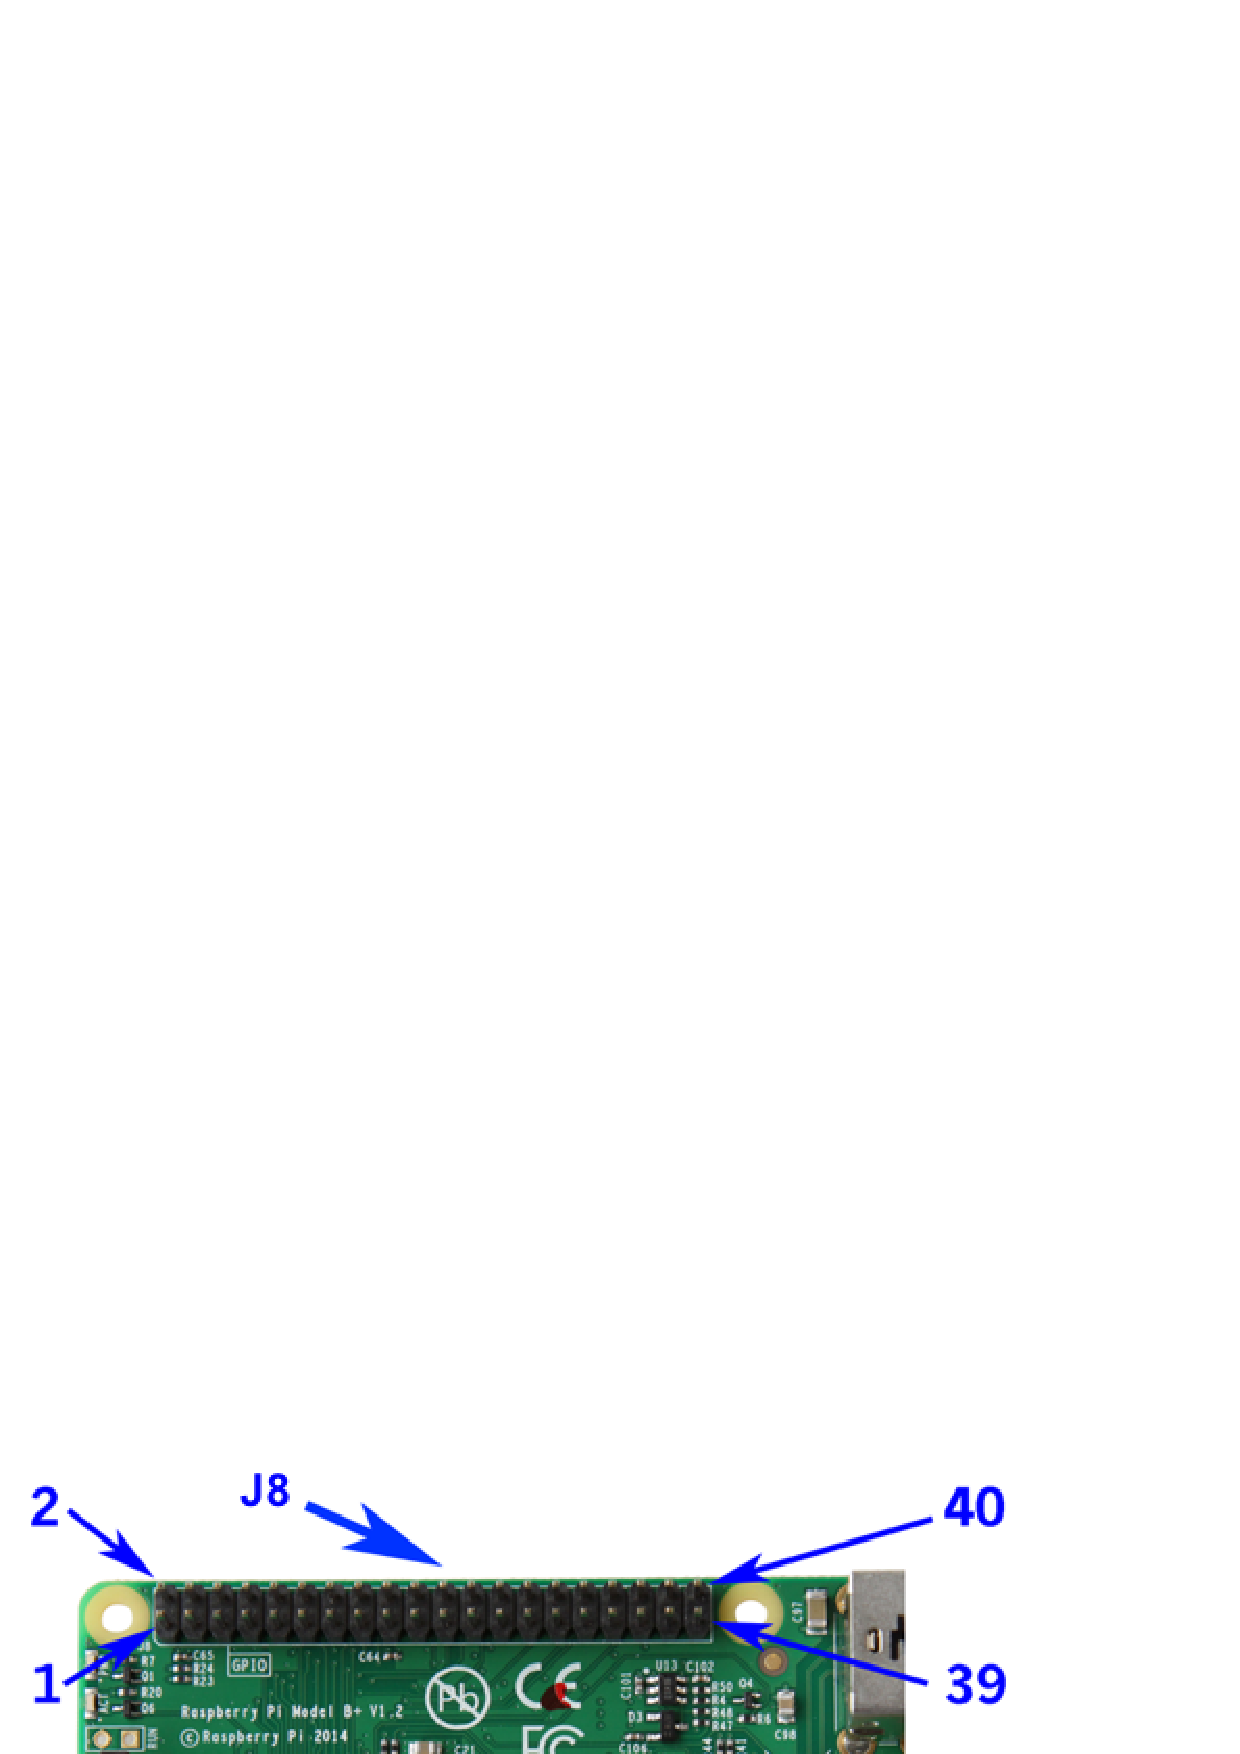
\includegraphics[width=\columnwidth]{./figs/gpio2}
\end{center}
\captionof{figure}{GPIO pin snapshot on Pi.}
\label{fig_1_3a}	
\end{figure}
%
\begin{figure}
\begin{center}
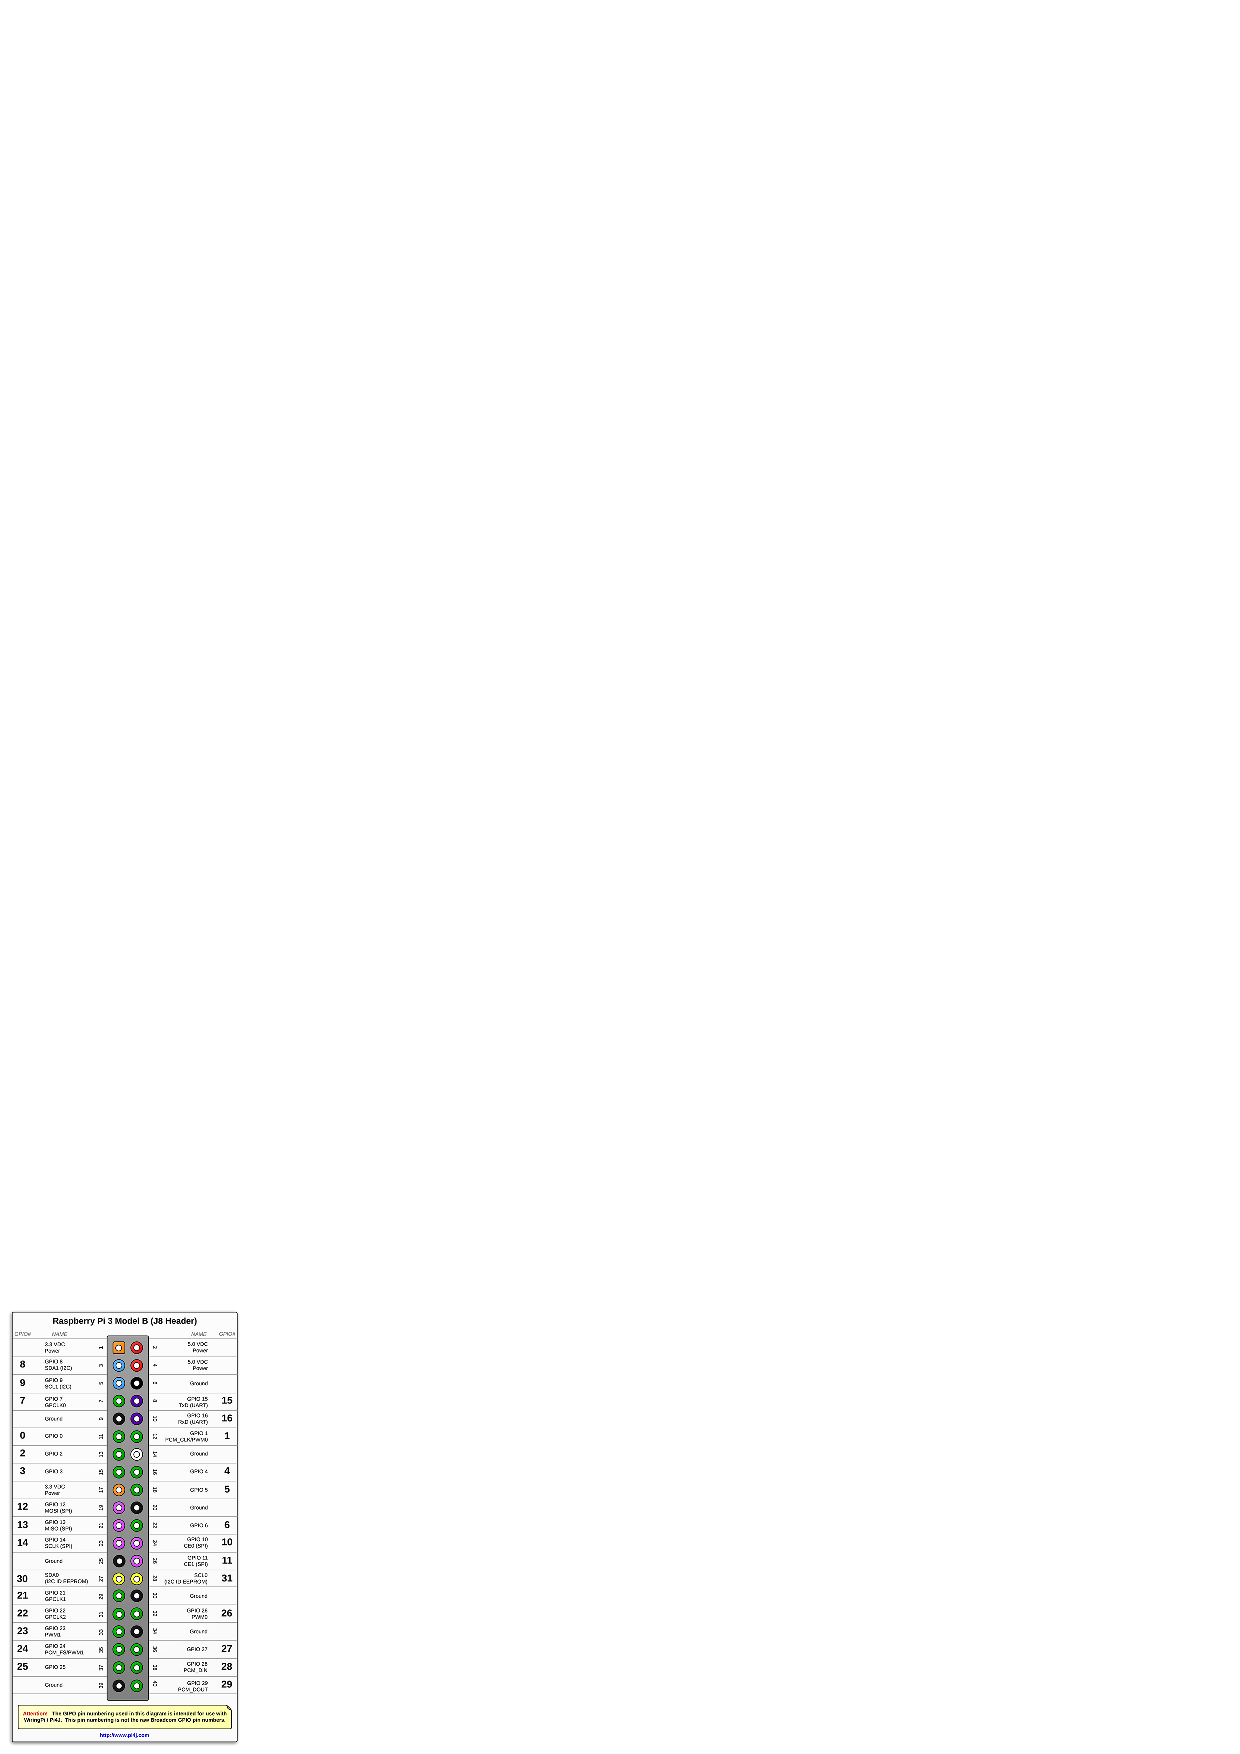
\includegraphics[width=\columnwidth]{./figs/gpio1}
\end{center}
\captionof{figure}{GPIO Wiring Pi pin configuration.}
\label{fig_1_3b}	
\end{figure}
\renewcommand{\thefigure}{\theproblem}
\begin{problem}
Connect the a-g pins of the display to the GPIO pins 0-6 of the Pi shown in \ref{fig_1_3a} and \ref{fig_1_3b}.
\end{problem}
\begin{problem}
Type the following C code and excute. What do you observe?
\end{problem}
\solution
\lstinputlisting[language=C]{./code/seven_seg_disp.c}
\begin{problem}
Now generate the numbers 0-9 by modifying the above program.
\end{problem}
\begin{problem}
Suitably modify the above program to obtain a decade counter.
\end{problem}


%\begin{problem}
%\label{prob:first_code}
%%Type the following code and execute. What do you observe?
%%\lstinputlisting[language=C]{./codes/bcd_seven.c}
%%// the setup function runs once when you press reset or power the board
int a=1,b=0,c=0,d=1,e=1,f=1,g=1;
void setup() {
    pinMode(2, OUTPUT);  
    pinMode(3, OUTPUT);
    pinMode(4, OUTPUT);
    pinMode(5, OUTPUT);
    pinMode(6, OUTPUT);
    pinMode(7, OUTPUT);
    pinMode(8, OUTPUT);            
}

// the loop function runs over and over again forever
void loop() {
  
  digitalWrite(2, a); 
  digitalWrite(3, b); 
  digitalWrite(4, c); 
  digitalWrite(5, d); 
  digitalWrite(6, e); 
  digitalWrite(7, f);     
  digitalWrite(8, g); 
}


%\end{problem}
%\begin{problem}
%Now generate the numbers 0-9 by modifying the above program.
%\end{problem}
%%
%%\newpage

%%\section{Combinational Logic}
%%
%\subsection{Counting Decoder}
	%In the  truth table in Table \ref{table:counter_decoder},  $W,X,Y,Z$ are the inputs
%and $A,B,C,D$ are the outputs. This table represents the system that increments the numbers 0-8 by 1 and resets the number 9 to 0
%%
%Note that  $D = 1$ for the inputs $0111$ and $1000$.  Using {\em boolean} logic,
%%
%\begin{equation}
%\label{bool_logic}
%D = WXYZ^{'} + W^{'}X^{'}Y^{'}Z
%\end{equation}
%%
%Note that $0111$ results in the expression $WXYZ^{'}$ and $1000$ yields $W^{'}X^{'}Y^{'}Z$. 
%%The $\&\&$ operand is used for the boolean AND (multiplication) operation, the $||$ operand is used for the OR (addition) operation and the ! operand is used for the NOT ($^{'}$) operation in Arduino code.  For example, the expression for \eqref{bool_logic} in Arudino is
%%\begin{verbatim}
%%D = (W&&X&&Y&&!Z)||(!W&&!X&&!Y&&Z);
%%\end{verbatim}

%\begin{problem}
	%\label{counter_dec}

%Write the boolean logic functions for $A,B,C$ in terms of $W,X,Y,Z$.
%\end{problem}
%%
%\input{./figs/counter_decoder}
%%
%%
%\begin{problem}
%%	\label{D_code}
%Write a program for implementing Table \ref{counter_dec}.
%%\eqref{bool_logic} in Arduino.
%\end{problem}
%%
%\solution
%%\lstinputlisting[language=C]{./codes/count_decoder.c}
%%
%%\begin{problem}
%%Modify the above program by keeping W=0,X=0,Y=0,Z=1 and A=1 and execute.  Verify that your results are consistent with Table \ref{counter_dec}.
%%\end{problem}

%\begin{problem}
%Verify if your logic is correct by observing the output on the seven segment display for different inputs.
%\end{problem}
%%
%\begin{problem}
%Connect GPIO pin 10 to the dot pin of the display and execute the following code.
%\end{problem}
%%\lstinputlisting[language=C]{./codes/blink.c}
%%
%%
%\begin{problem}
%A decade counter counts the numbers from 0-9 and then resets to 0.  Suitable modify the above programs to obtain a decade counter.
%\end{problem}

%\subsection{Display Decoder}
%%
%\begin{problem}
%Now write the truth table for the seven segment display decoder (IC 7447).  The inputs will be $A,B,C,D$ and the outputs will be $a,b,c,d,e,f,g$.
%\end{problem}
%%
%\begin{problem}
%\label{seven_seg_disp_logic}
%Obtain the logic functions for outputs $a,b,c,d,e,f,g$ in terms of the inputs $A,B,C,D$.
%\end{problem}
%\begin{problem}
%Disconnect the Pi from IC 7447 and connect the pins GPIO 0-6 in the Pi directly to the seven segment display.
%\end{problem}
%\begin{problem}
%Write a new program to implement the logic in Problem \ref{seven_seg_disp_logic} and observe the output in the display.  You have designed the logic for IC 7447!
%\end{problem}
%\begin{problem}
%Now include your counting decoder program in the  display decoder program
%and see if the display shows the consecutive number.
%\end{problem}
%A decade counter counts the numbers from 0-9 and then resets to 0.
%\begin{problem}
%Suitably modify the above program to obtain a decade counter.
%\end{problem}




%\begin{problem}
%Generate the boolean functions for the segments $a-f$ using the table in Problem \ref{bcd_ss}.  For example, the function for $a$ is obtained from the table as
%\begin{equation}
%a=\bar{D}\bar{C}\bar{B}A+\bar{D}C\bar{B}\bar{A}
%\label{boolean}
%\end{equation}
%\end{problem}
%%
%\begin{problem}
	%\label{counter_dec}
%Write functions for $A,B,C,D$ in Arduino using the following table and verify using the Arduino driven display.
		%\input{counter_decoder}
%\end{problem}
%\begin{problem}
	%Write a module for decimal to binary conversion
	%according to the example given below
	%\input{conversion}
	%%
	%$N \% 2$ gives the remainder and $N/2$ gives the quotient
%	and use it in the above code so that decimal values are given as input in the program and observed as output in the display. Note that the following code
%	\begin{verbatim}
%	a % b
%	\end{verbatim}
%	can be used to obtain the remainder when a is divided by b and
%	\begin{verbatim}
%	a/b
%	\end{verbatim}
%	gives the quotient.
%\end{problem}
 
%%
%\newpage
%\section{$M$-ary Modulation}
%\subsection{Angle Bisectors}

\begin{figure}[!h]
	\begin{center}
		
		%
\includegraphics[width=\columnwidth]{./figs/ch3_angle_bisector}
		%\vspace*{-10cm}
		\resizebox{\columnwidth}{!}{\begin{tikzpicture}
[scale=2,>=stealth,point/.style={draw,circle,fill = black,inner sep=0.5pt},]

\node (D) at (0, 0)[point,label=below :$D$] {};
\node (A) at (0, 3)[point,label=above :$A$]{};
\node (B) at (-3, 0)[point,label=below left:$B$]{};
\node (C) at (3, 0)[point,label=below right:$C$]{};
\node (O) at (0, 1.3)[point,label=below right:$O$]{};
\node (F) at (-1.1, 1.9)[point,label=above left:$F$]{};
\node (E) at (1.1, 1.9)[point,label=above right:$E$]{};

\draw (D)--(B);
\draw (B)--(A);
\draw (A)--(C);
\draw (C)--(D);
\draw [thick,dashed] (A) -- (D);
\draw [thick,dashed] (O) -- (E);
\draw [thick,dashed] (O) -- (F);
\draw (B)--(O);
\draw (C)--(O);

\tkzMarkRightAngle[size=.2](A,D,C)
\tkzMarkRightAngle[size=.15](B,F,O);
\tkzMarkRightAngle[size=.15](C,E,O);
\tkzMarkAngle[size=.4](D,B,O);
\tkzMarkAngle[size=.35](O,B,F);
\tkzMarkAngle[size=.54](E,C,O);
\tkzMarkAngle[size=.5](E,C,O);
\tkzMarkAngle[size=.6](O,C,D);
\tkzMarkAngle[size=.65](O,C,D);

\end{tikzpicture}}
	\end{center}
	\caption{Angle bisectors meet at a point}
	\label{ch3_angle_bisector}	
\end{figure}

\begin{definition}
	In Fig. \ref{ch3_angle_bisector}, $OB$ divides the  $\angle B$ into half, i.e.\begin{equation}
	\angle OBC = \angle OBA
	\end{equation}
	$OB$ is known as an angle bisector.
\end{definition}
	$OB$ and $OC$ are angle bisectors of angles $B$ and $C$. $OA$ is joined and $OD, OF$ and $OE$ are perpendiculars to sides $a,b$ and $c$.
\begin{problem}
  Show that $OD = OE = OF$.
\end{problem}
\proof In $\Delta$s $ODC$ and $OEC$,
\begin{align}
OD &= OC \sin \frac{C}{2}
\\
OE &= OC \sin \frac{C}{2} 
\\
\Rightarrow OD &=OE.
\end{align}
Similarly,
\begin{equation}
OD = OF.
\end{equation}
%
\begin{problem}
	Show that OA is the angle bisector of $\angle A$
\end{problem}
\proof In $\Delta$s $OFA$ and $OEA$,
\begin{align}
OF &= OE
\\
\Rightarrow OA \sin OAF &= OA \sin OAE \\
\Rightarrow \sin OAF &=  \sin OAE \\
\Rightarrow \angle OAF &= \angle OAE
\end{align}
which proves that $OA$ bisects $\angle A$.
{\em Conclusion:} The angle bisectors of a triangle meet at a point.


\subsection{Congruent Triangles}
%
\begin{problem}
	Show that in $\Delta$s $ODC$ and $OEC$, corresponding sides and angles are equal.
\end{problem}
\begin{definition}
	Note that    $\Delta$s $ODC$ and $OEC$ are known as congruent triangles.  To show that two triangles are congruent, it is sufficient to show that some angles and sides are equal.
\end{definition}
\begin{problem}
SSS:	Show that if the corresponding sides of three triangles are equal, the triangles are congruent.
\end{problem}
\begin{problem}
ASA:	Show that if two angles and any one side  are equal in corresponding triangles, the triangles are congruent.
\end{problem}
\begin{problem}
SAS:	Show that if two sides and the angle between them are equal in corresponding triangles, the triangles are congruent.
\end{problem}
\begin{problem}
RHS:	For two right angled triangles, if the hypotenuse and one of the sides are equal, show that the triangles are congruent.
\end{problem}
	%
%%
\subsection{Perpendicular Bisectors}
\begin{definition}
	In Fig. \ref{ch3_perp_bisector}, OD $\perp BC$ and $BD=DC$. $OD$ is defined as the perpendicular bisector of $BC$.
\end{definition}

\begin{problem}
	In Fig. \ref{ch3_perp_bisector}, show that $OA=OB=OC$.
\end{problem}
%%
%%
\begin{figure}[!h]
	\begin{center}
		
		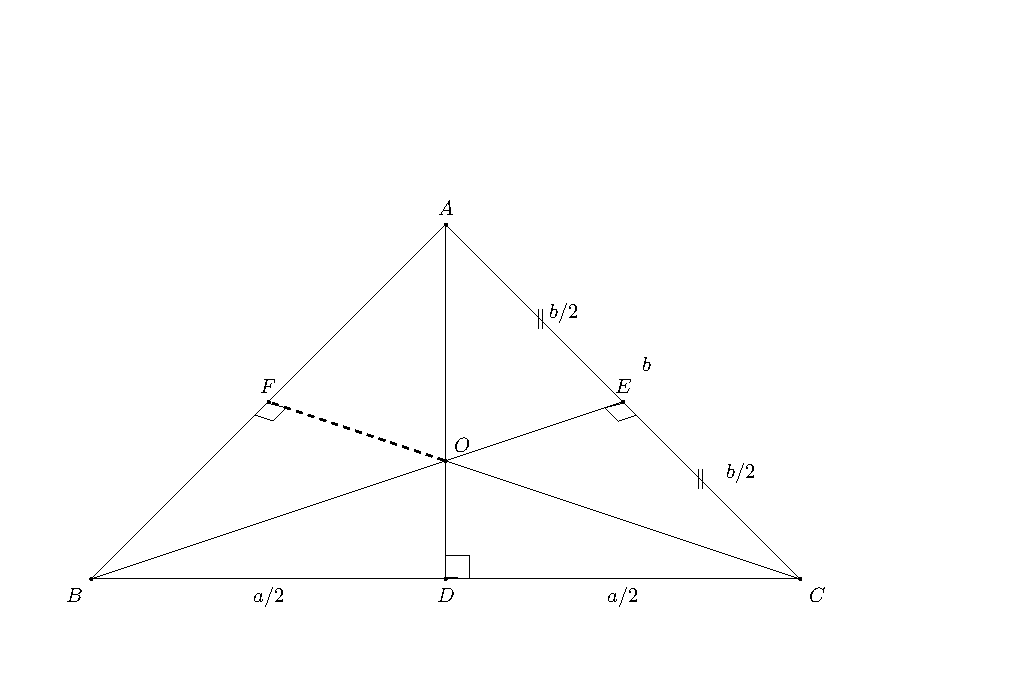
\includegraphics[width=\columnwidth]{./figs/fig_3.8.eps}
%		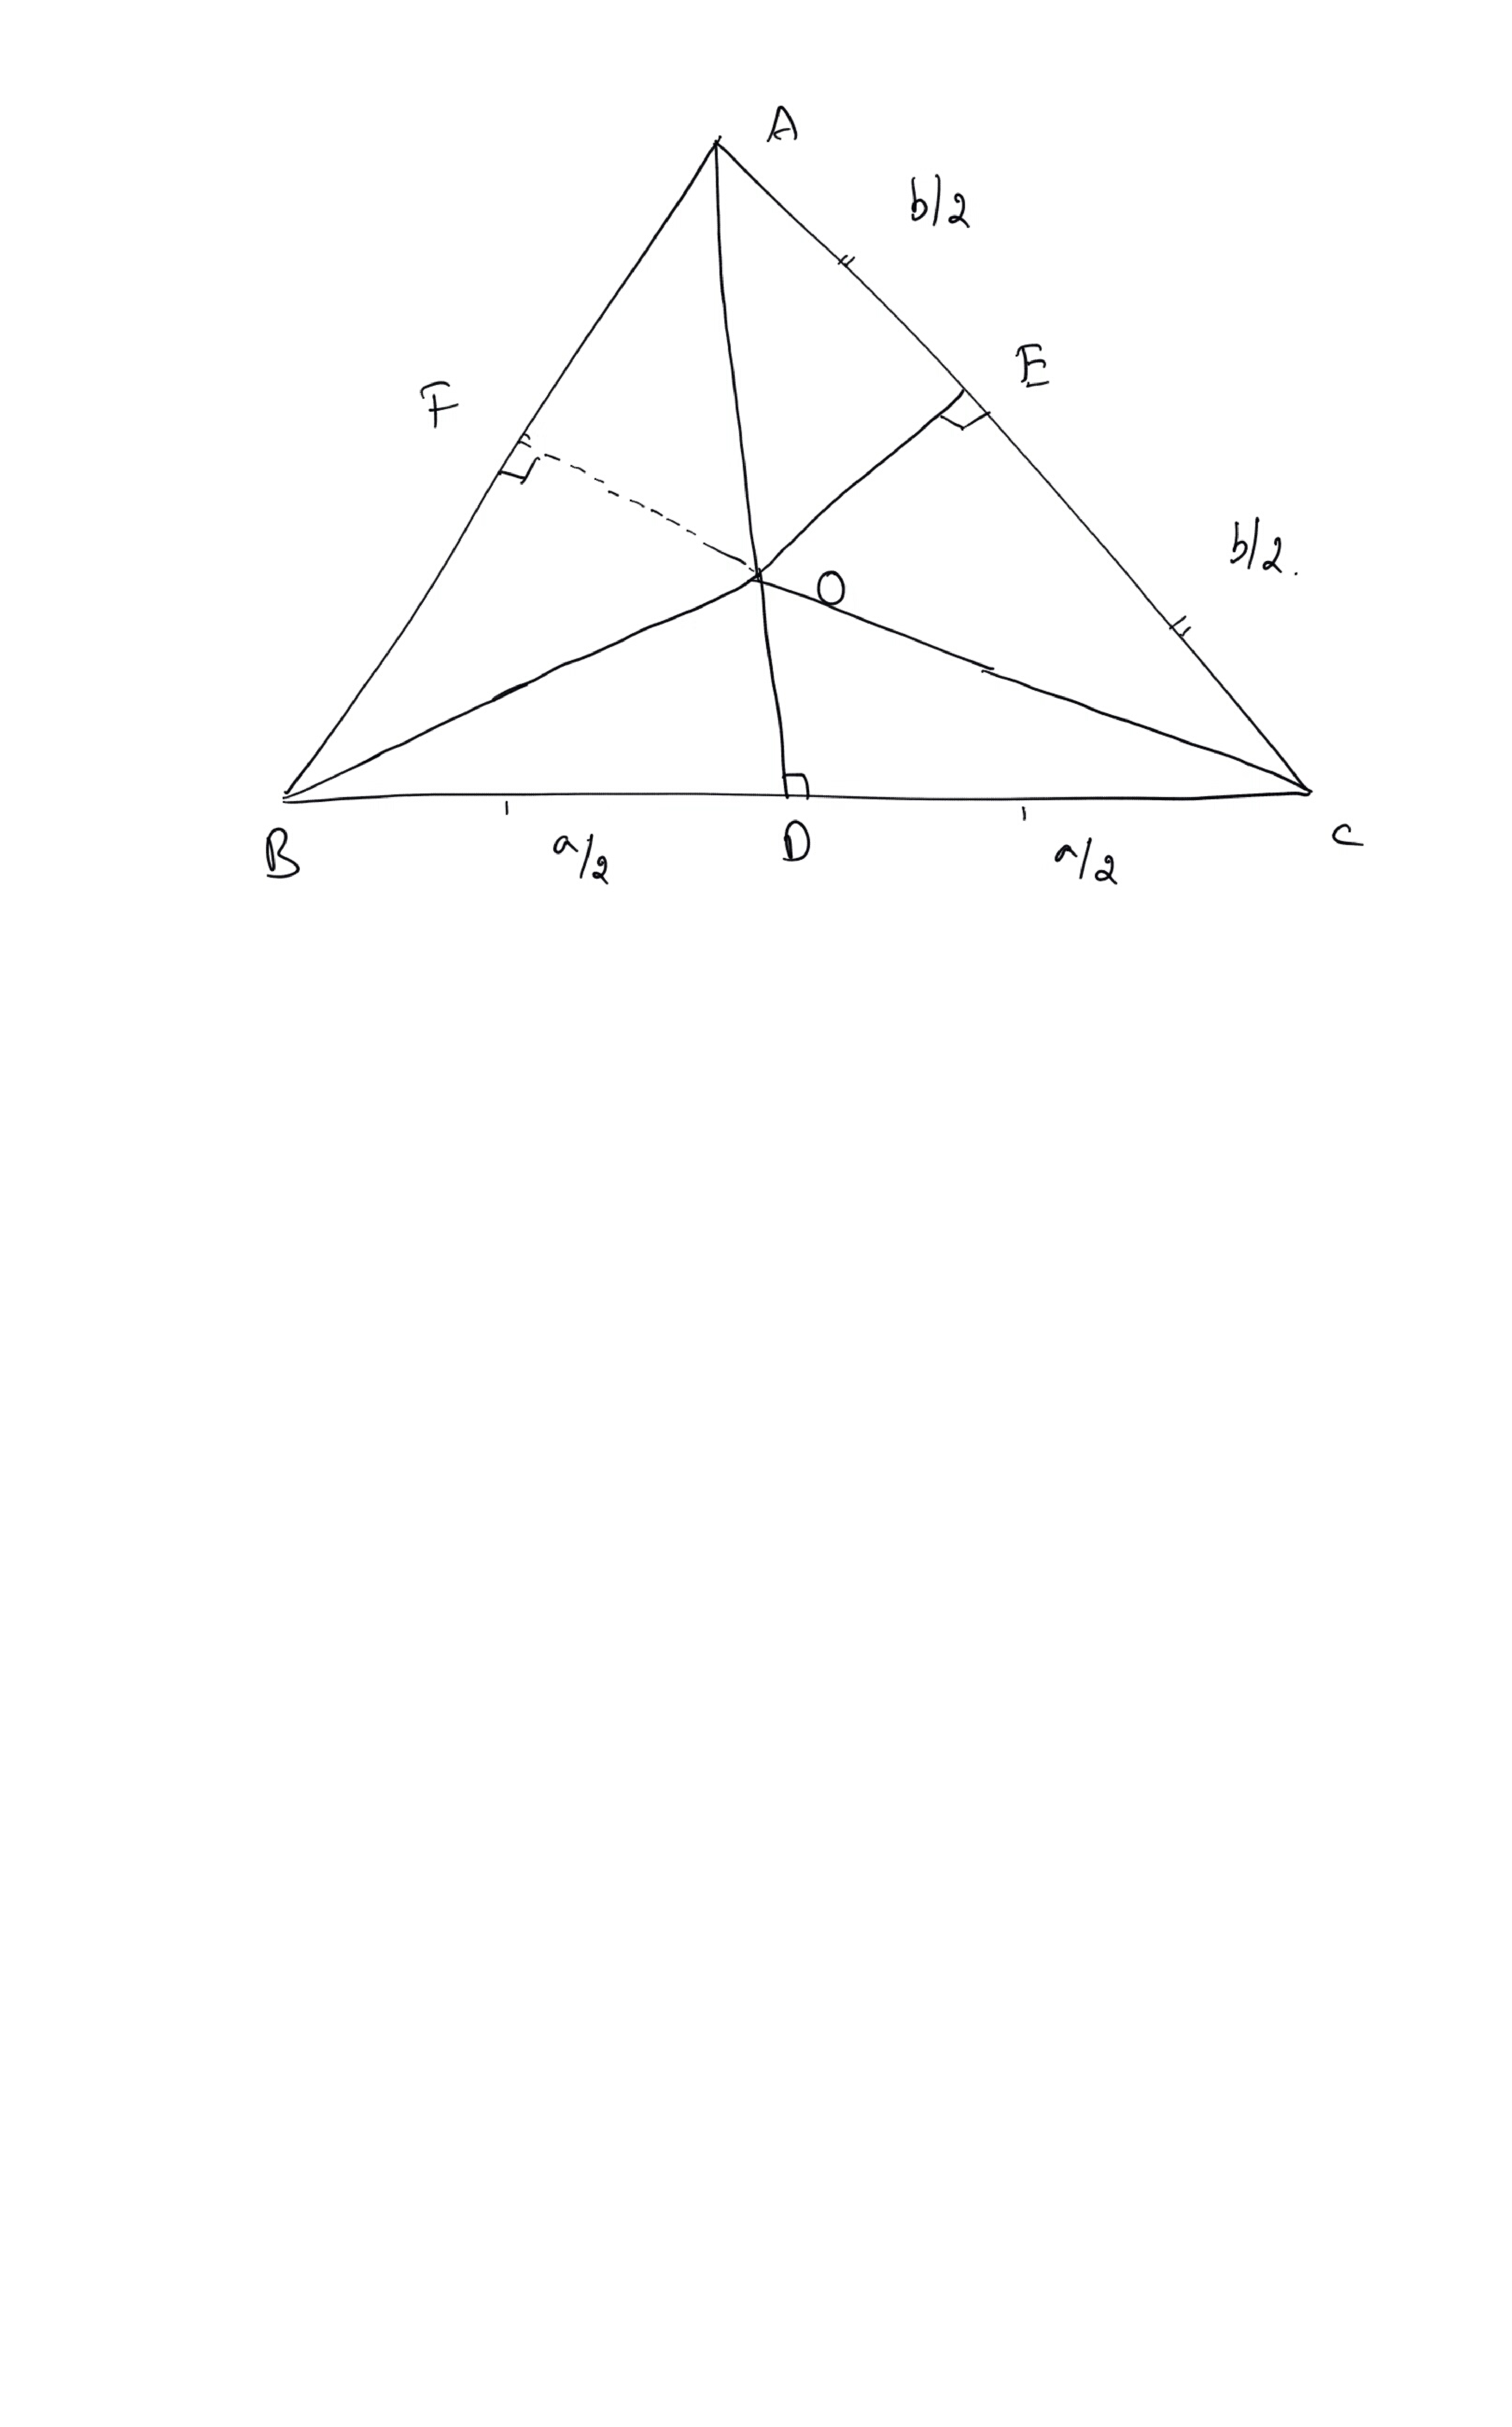
\includegraphics[width=\columnwidth]{./figs/ch3_perp_bisector}
		%\vspace*{-10cm}
%		\resizebox{\columnwidth}{!}{\documentclass{standalone}
\usepackage{tikz}
\usepackage{tkz-euclide}
\usetkzobj{all}
%\usepackage{amsmath}
\providecommand{\brak}[1]{\ensuremath{\left(#1\right)}}

\begin{document}
\begin{tikzpicture}
[scale=2,>=stealth,point/.style={draw,circle,fill = black,inner sep=0.5pt},]

\node (E) at (1.5, 1.5)[point,label=above :$E$] {};
\node (F) at (-1.5, 1.5)[point,label=above :$F$] {};
\node (A) at (0, 3)[point,label=above :$A$]{};
\node (B) at (-3, 0)[point,label=below left:$B$]{};
\node (C) at (3, 0)[point,label=below right:$C$]{};
\node (D) at (0,0)[point,label=below :$D$] {};
\node (O) at (0,1)[point,label=above right :$O$] {};


\draw (B)--(A);
\draw (A)--(C);
\draw (B)--(C);
\draw (B)--(E);
\draw (C)--(O);
\draw (A)--(D);
\draw [thick,dashed] (O) -- (F);

\node [above] at (1.7,1.7) {$b$};
\node [above] at (2.5,.75) {$b/2$};
\node [above] at (1,2.1) {$b/2$};
\node [above] at (-1.5,-0.3){$a/2$};
\node [above] at (1.5,-0.3){$a/2$};
\tkzMarkRightAngle[size=.16](B,F,O)
\tkzMarkRightAngle[size=.16](C,E,O)
\tkzMarkRightAngle[size=.2](A,D,C)
\draw   -- (4.3,1.7) node[midway] {$\parallel$};
\draw   -- (1.6,4.4) node[midway] {$\parallel$};

\end{tikzpicture}
\end{document}}
	\end{center}
	\caption{Perpendicular bisectors meet at a point}
	\label{ch3_perp_bisector}	
\end{figure}
%
\proof In $\Delta$s $ODB$ and $ODC$, using Budhayana's theorem,
%
\begin{equation}
\begin{split}
OB^2 &= OD^2 + BD^2 \\
OC^2 &= OD^2 + DC^2 
\end{split}
\end{equation}
%
Since $BD = DC = \frac{a}{2}$, $OB = OC$.  Similarly, it can be shown that $OA = OC$.  Thus, $OA=OB=OC$.
%
\begin{definition}
	In $\Delta AOB$, $OA = OB$.  Such a triangle is known as an isoceles triangle.
\end{definition}
%
\begin{problem}
	Show that $AF = BF$.
\end{problem}
\proof Trivial using Budhayana's theorem.  This shows that $OF$ is a perpendicular bisector of $AB$. 
{\em Conclusion:}  The perpendicular bisectors of a triangle meet at a point.
%
\subsection{Perpendiculars from Vertex to Opposite Side}
	%
	%
	In Fig. \ref{ch3_perp_triang}, $AD \perp BC$ and $BE \perp AC$. $CF$ passes through $O$ and meets
	$AB$ at $F$.  	
\begin{problem}
	Show that 
	\begin{align}
	OE = c \cos A \cot C
	\end{align}
\end{problem}
	\begin{figure}[!h]
		\begin{center}
			
			%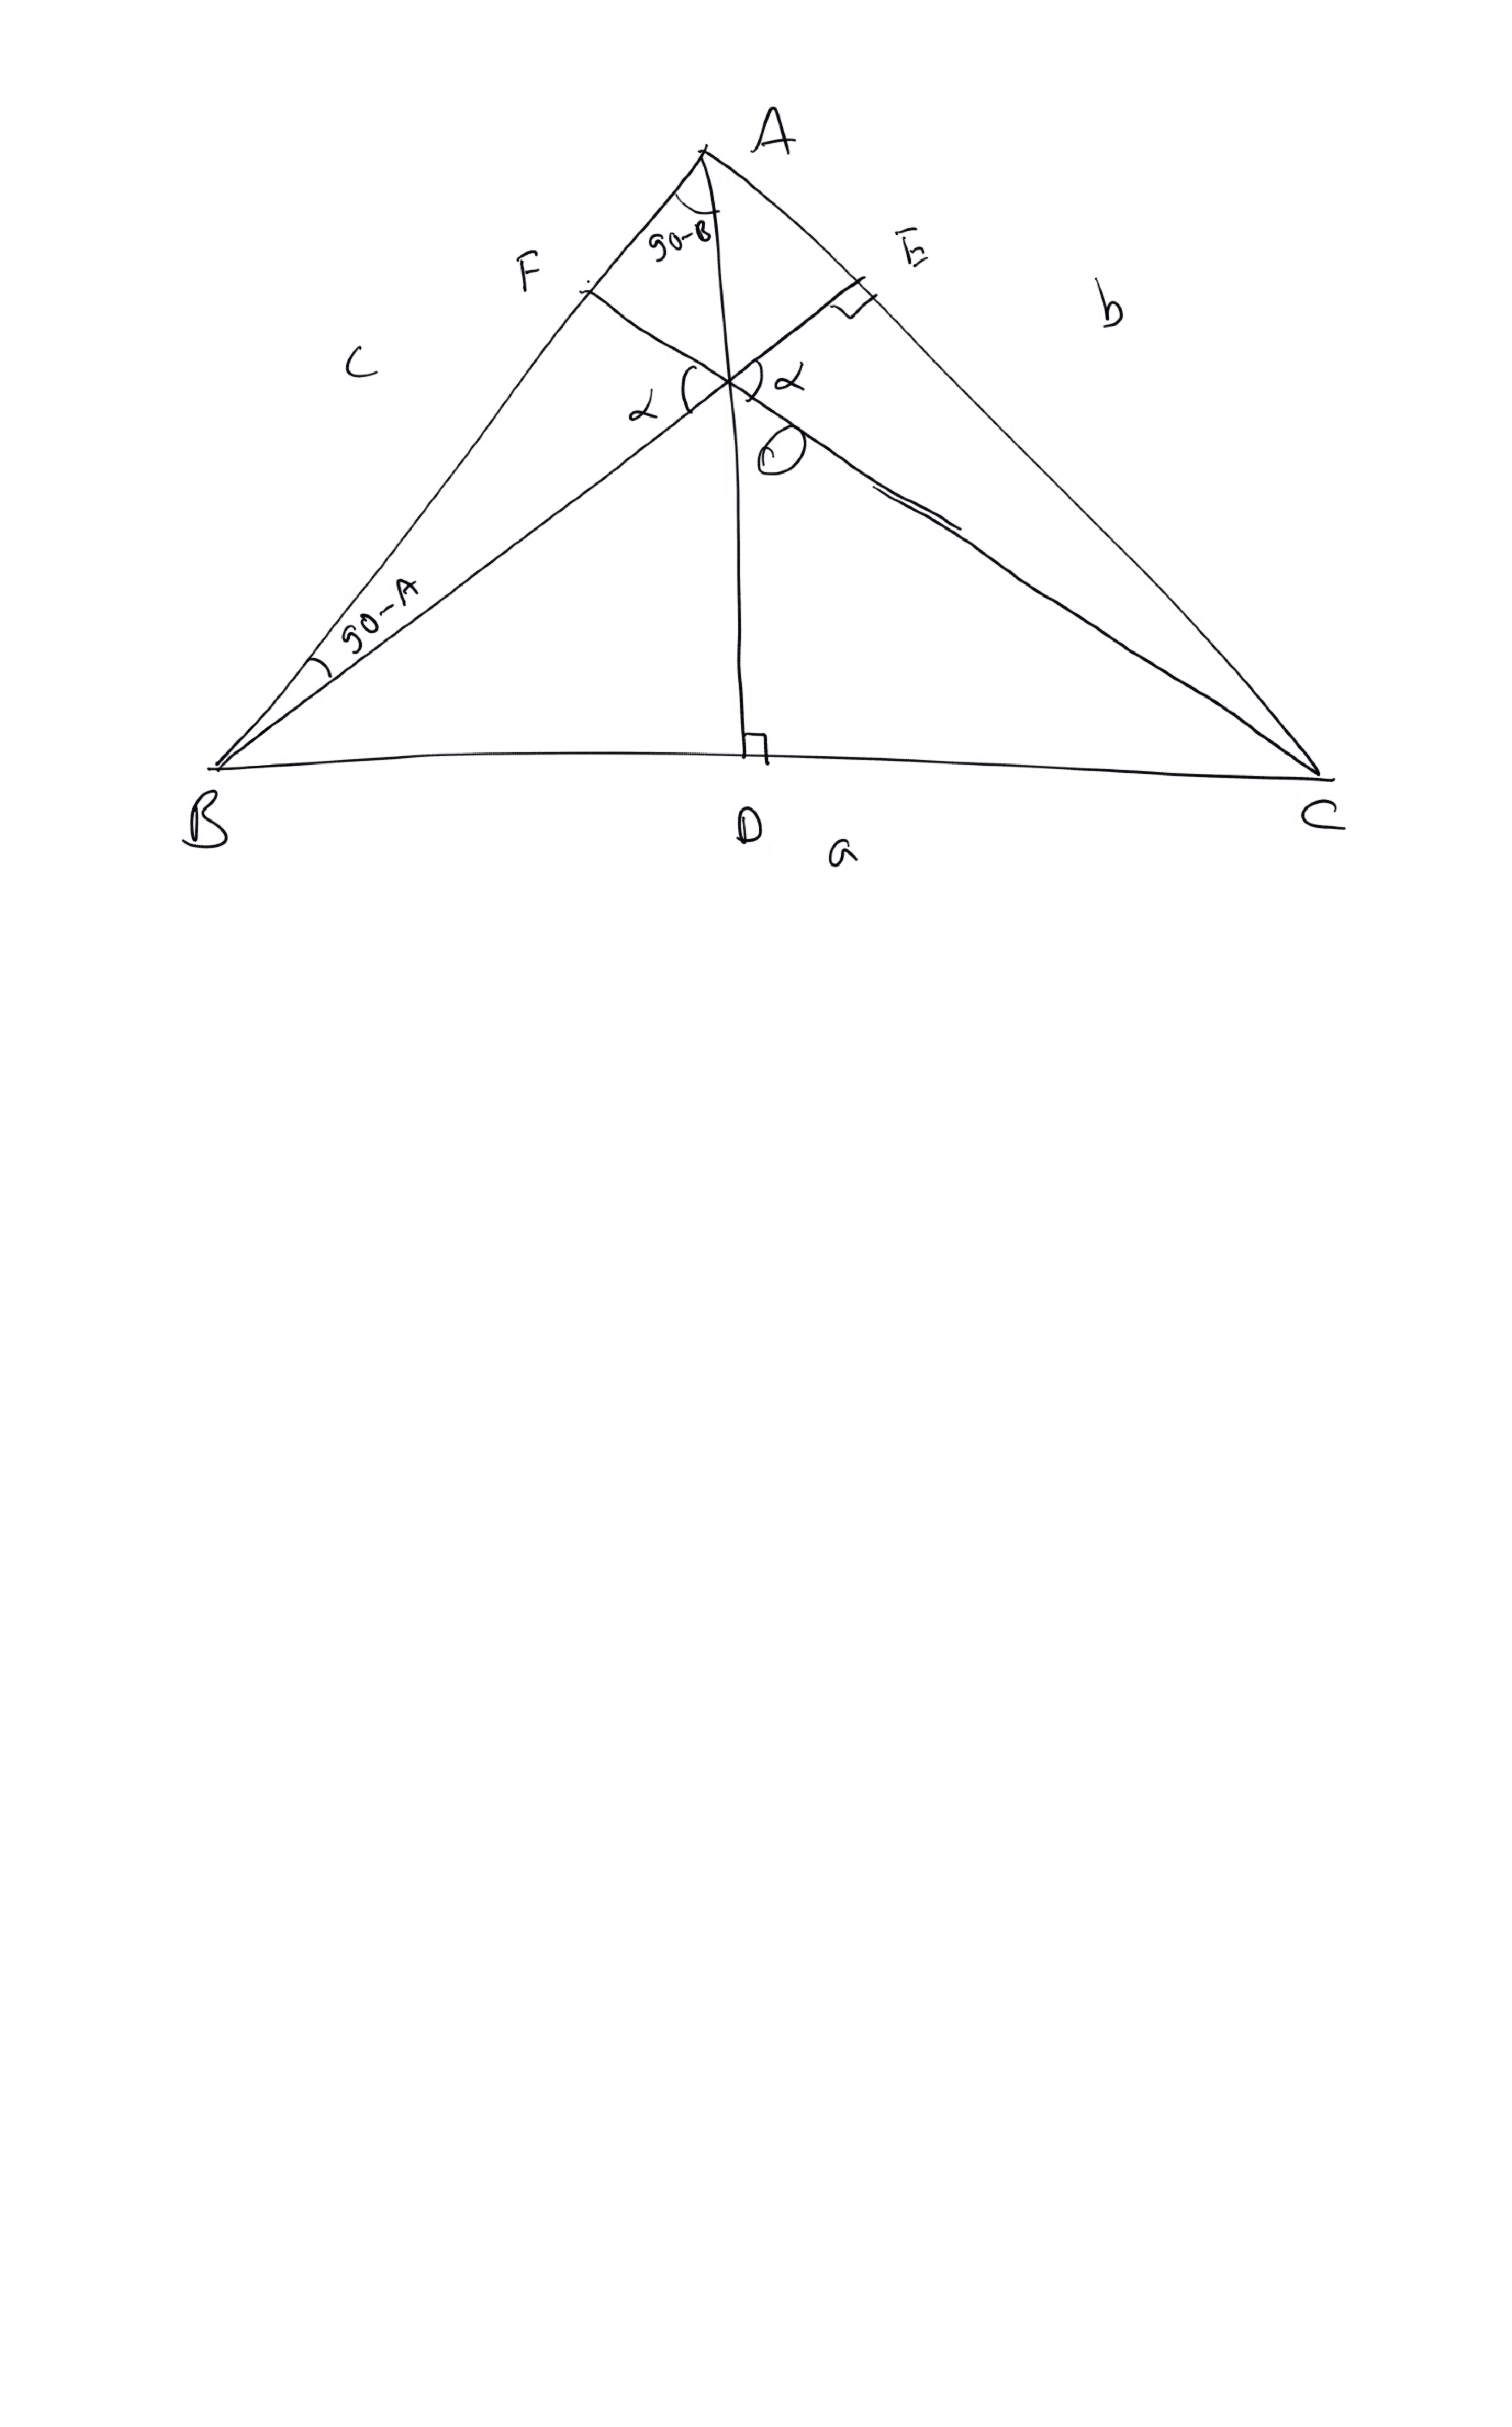
\includegraphics[width=\columnwidth]{./figs/ch3_perp_triang}
			%\vspace*{-10cm}
			\resizebox{\columnwidth}{!}{\begin{tikzpicture}
[scale=2,>=stealth,point/.style={draw,circle,fill = black,inner sep=0.5pt},]

\node (E) at (1.5, 1.5)[point,label=above :$E$] {};
\node (F) at (-1.5, 1.5)[point,label=above :$F$] {};
\node (A) at (0, 3)[point,label=above :$A$]{};
\node (B) at (-3, 0)[point,label=below left:$B$]{};
\node (C) at (3, 0)[point,label=below right:$C$]{};
\node (O) at (0,1)[point,label=above right :$O$] {};
\node (D) at (0,0)[point,label=below :$D$] {};


\draw (B)--(A);
\draw (A)--(C);
\draw (B)--(E);
\draw (C)--(F);
\draw (B)--(C);
\draw (A)--(D);

\node [below] at (0,-0.3) {$a$};
\node [above] at (-1.7,1.7) {$c$};
\node [above] at (1.7,1.7) {$b$};
\node [above] at (1,1.3) {$p$};
\node [above] at (-1,1.3) {$q$};
\node [above] at (-2.3,0.24){\rotatebox{45}{$90-A$}};
\node [above] at (-0.4,2.1) {\rotatebox{45}{$90-B$}};
\node [above] at (0.4,2.1) {\rotatebox{-45}{$90-C$}};

\tkzMarkAngle[size=.3](F,O,B);
\tkzMarkAngle[size=.3](C,O,E);
\tkzMarkAngle[size=.4](O,B,F);
\tkzMarkAngle[size=.2](F,A,O);
\tkzMarkAngle[size=.3](O,A,E);
\draw (-0.5,1) node{$\alpha$};
\draw (0.5,1) node{$\alpha$};

\end{tikzpicture}
}
		\end{center}
		\caption{Perpendiculars from vertex to opposite side meet at a point}
		\label{ch3_perp_triang}	
	\end{figure}
%
\proof In $\Delta$ s $AEB$ and $AEO$,
%
\begin{align}
AE &= c \cos A \\
OE &= AE \tan \brak{90^{\degree} - C} \brak{\because ADC \text{ is right angled}} \\
&= AE \cot C
\end{align}
%
From both the above, we get the desired result.
%
\begin{problem}
	Show that $\alpha = A$.
\end{problem}
\proof In $\Delta OEC$,
%
\begin{equation}
CE = a \cos C \brak{\because BEC \text{ is right angled}}
\end{equation}
%
Hence,
%
\begin{equation}
\begin{split}
\tan \alpha &= \frac{CE}{OE} \\
&=  \frac{a \cos C}{c \cos A \cot C} \\
&=  \frac{a \cos C \sin C}{c \cos A \cos C} \\
&= \frac{a \sin C}{c \cos A } \\
&= \frac{c \sin A}{c \cos A } \brak{\because \frac{a}{\sin A} = \frac{c}{\sin C}}\\
&= \tan A\\
\Rightarrow \alpha = A
\end{split}
\end{equation}
%
\begin{problem}
	Show that $CF \perp AB$
\end{problem}
\proof Consider triangle OFB and the result of the previous problem.  $\because$ the sum of the angles of a triangle is $180^{\degree}$, $\angle CFB = 90^{\degree}$.
{\em Conclusion: The perperdiculars from the vertex of a triangle to the opposite side meet at a point.} 
%
%\newpage
%\section{BER in Rayleigh Flat Slowly Fading Channels}
	%\subsection{Chord of a Circle}

\begin{figure}[!h]
	\begin{center}
		
		
\includegraphics[width=\columnwidth]{./figs/ch4_circle_def}
		\vspace*{-10cm}
	\end{center}
	\caption{Circle Definitions}
	\label{ch4_circle_def}	
\end{figure}
\begin{definition}
	Fig. \ref{ch4_circle_def} represents a circle.  The points in the circle are at a distance $r$ from the centre $O$.  $r$ is known as the radius.
\end{definition}

\subsection{Chords of a circle}
\begin{definition}
	In Fig. \ref{ch4_circle_def}, $A$ and $B$ are points on the circle.  The line $AB$ is known as a chord of the circle.
\end{definition}
%
%
\begin{problem}
	\label{ch4_prob_circle_subtend}
	In Fig. \ref{ch4_circle_subtend}  Show that $\angle OAB = 2\angle APB $.
\end{problem}
\begin{figure}[!h]
	\begin{center}
		
		
\includegraphics[width=\columnwidth]{./figs/ch4_circle_subtend}
		\vspace*{-10cm}
	\end{center}
	\caption{Angle subtended by chord $AB$ at the centre $O$ is twice the angle subtended at $P$. }
	\label{ch4_circle_subtend}	
\end{figure}

\proof In Fig. \ref{ch4_circle_subtend}, the triangeles $OPA$ and $OPB$ are isosceles. Hence,
%
\begin{align}
\angle OPB = \angle OBP &= \theta_1 \\
\angle OPA = \angle OAP &= \theta_2
\end{align}
%
Also, $\alpha$ and $\beta$ are exterior angles corresponding to the triangle $OPB$ and $OPA$ respectively. Hence
%
\begin{align}
\alpha &= 2\theta_1 \\
\beta &= 2\theta_2
\end{align}
%
Thus,
%
\begin{align}
\angle AOB &= \alpha + \beta \\
&= \theta_1 + \theta_2 \\
&= \angle APB
\end{align}
%
\begin{definition}
	The diameter of a circle is the chord that divides the circle into two equal parts. In Fig. \ref{ch4_circle_dia}, $AB$ is the diameter and passes through the centre $O$
\end{definition}
%
\begin{problem}
In Fig. \ref{ch4_circle_dia}, show that $\angle APB = 90^{\degree}$ .
\end{problem}
%
\begin{figure}[!h]
	\begin{center}
		
		
\includegraphics[width=\columnwidth]{./figs/ch4_circle_dia}
		\vspace*{-10cm}
	\end{center}
	\caption{Diameter of a circle.}
	\label{ch4_circle_dia}	
\end{figure}

\begin{problem}
	In Fig. \ref{ch4_chord_product}, show that 
	\begin{equation}
	\begin{split}
\angle ABD &= \angle ACD \\
\angle CAB &= \angle CDB	
	\end{split}
	\end{equation}
\end{problem}
\begin{figure}[!h]
	\begin{center}
		
		
\includegraphics[width=\columnwidth]{./figs/ch4_chord_product}
		\vspace*{-10cm}
	\end{center}
	\caption{$PA.PB = PC.PD$}
	\label{ch4_chord_product}	
\end{figure}
%
%
\proof Use Problem \ref{ch4_prob_circle_subtend}.
%
\begin{problem}
	In Fig. \ref{ch4_chord_product}, show that the triangles $PAB$ and $PBD$ are similar
\end{problem}
\proof Trivial using previous problem
\begin{problem}
	In Fig. \ref{ch4_chord_product}, show that 
	\begin{equation}
	PA.PB = PC.PD
	\end{equation}
\end{problem}
%
\proof Since triangles $PAC$ and $PBD$ are similar, 
%
\begin{align}
\frac{PA}{PD} &= \frac{PC}{PB} \\
\Rightarrow PA.PB &= PC.PD
\end{align}
%
%
\begin{definition}
	The line $PX$ in Fig. \ref{ch4_tangent_def} touches the circle at exactly one  point $P$. It is known as the tangent to the circle.
\end{definition}
%
%
\begin{problem}
	$OP$ is the perpendicular to the line $PX$ as shown in the Fig. \ref{ch4_short_dist}. Show that $OP$ is the shortest distance between the point $O$ and the line $PX$. 
\end{problem}
\proof Let $P_1$ be a point on the line $PX$. Then $OPP_1$ is a right angled triangle.  Using Budhayana's theorem,
%
\begin{figure}[!h]
	\begin{center}
		
		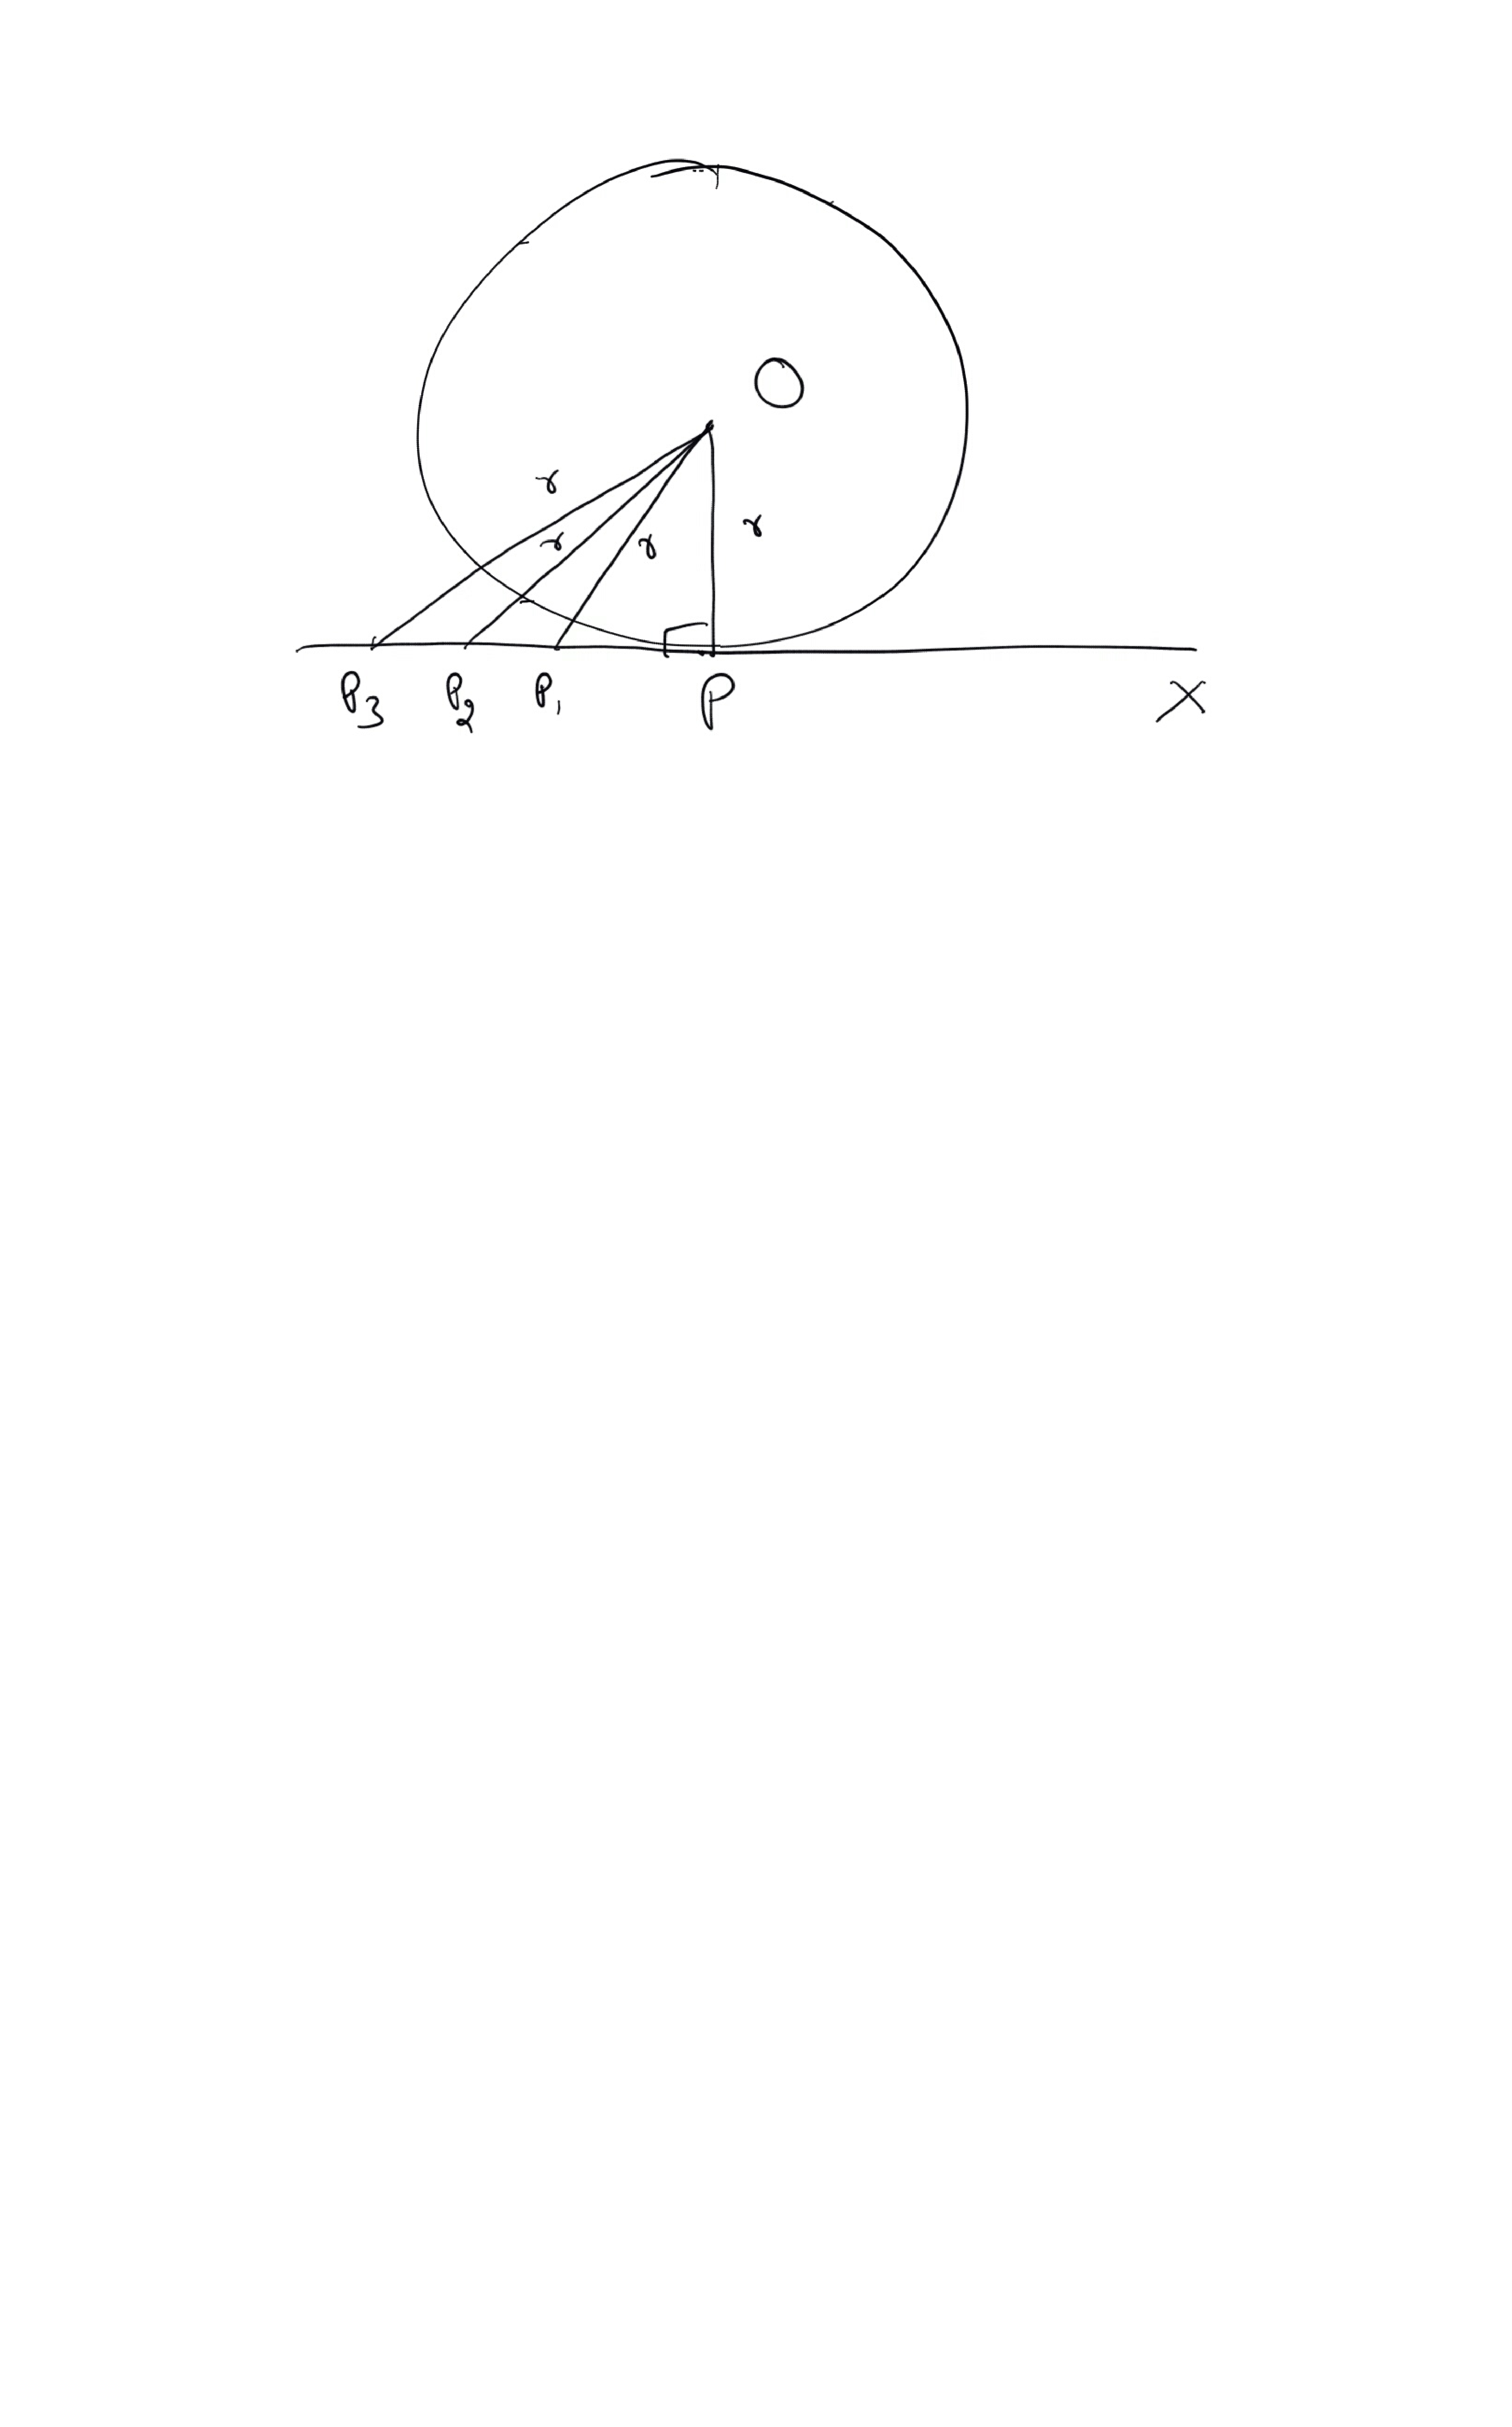
\includegraphics[width=\columnwidth]{./figs/ch4_tangent_def}
		\vspace*{-10cm}
	\end{center}
	\caption{Tangent to a Circle.}
	\label{ch4_tangent_def}	
\end{figure}
%
\begin{figure}[!h]
	\begin{center}
		
		
\includegraphics[width=\columnwidth]{./figs/ch4_short_dist}
		\vspace*{-10cm}
	\end{center}
	\caption{Shortest distance from $O$ to line $PX$}
	\label{ch4_short_dist}	
\end{figure}

%
\begin{equation}
\begin{split}
OP_1^2 &= OP^2 + PP_1^2 \\
\Rightarrow OP_1 > OP
\end{split}
\end{equation}
%
Thus, $OP$ is the shortest distance between $O$ and line $PX$.
%
\begin{problem}
Show that $\angle OPX = 90 ^{\degree}$
\end{problem}
\proof In Fig. \ref{ch4_tangent_def}, we can see that $OP$ is is the radius of the circle and the length of all line segments from $O$ to the line $PX > r$.  Using the result of the previous 
problem, it is obvious that $OP \perp PX$. 
%
	%
\begin{problem}
In Fig. \ref{ch4_tangent_prod} show that 
%
\begin{equation}
\angle PCA = \angle PBC
\end{equation}
%
$O$ is the centre of the circle and $PC$ is the tangent.
\end{problem}
	\begin{figure}[!h]
		\begin{center}
			
			
\includegraphics[width=\columnwidth]{./figs/ch4_tangent_prod}
			\vspace*{-10cm}
		\end{center}
		\caption{$PA.PB = PC^2$.}
		\label{ch4_tangent_prod}	
	\end{figure}
	%

%
\proof For convenience, greek letters are used for representing certain angles. Since $\Delta OAC$ is isosceles,
%
\begin{align}
2 \alpha + 2 \brak{\beta - \phi} &= 180^{\degree} \\
\Rightarrow  \alpha +  \brak{\beta - \phi} &= 90^{\degree} \\
\Rightarrow  \alpha +  \beta  &= 90^{\degree} + \phi
\end{align}
%
Since $theta$ is an exterior angle for the $\Delta ABC
$,
%
\begin{equation}
\theta = \alpha + \beta
\end{equation}
%
From both the above equations
%
\begin{equation}
\theta = 90^{\degree} + \phi
\end{equation}
%
Since PC is the tangent, 
%
\begin{equation}
\angle PCB = 90^{\degree} + \phi = \theta
\end{equation}
%
Considering the sum of angles in $\Delta PAC$ $\Delta PBC$,
%
\begin{align}
\angle P + \theta + \angle PCA &= 180^{\degree} \\
\angle P + \theta + \alpha &= 180^{\degree}
\end{align}
Hence,
%
\begin{equation}
\angle PCA = \alpha
\end{equation}
%
\begin{problem}
	In Fig. \ref{ch4_tangent_prod}, show that the triangles $PAC$ and $PBC$ are similar.
\end{problem}
\proof From the previous problem, it is obvious that corresponding angles of both triangles are equal.  Hence they are similar.
%
\begin{problem}
	Show that $PA.PB = PC^2$
\end{problem}
\proof Since $\Delta PAC \sim \Delta PBC$, their sides are in the same ratio.  Hence,
%
\begin{align}
\frac{PA}{PC} &= \frac{PC}{PB} \\
\Rightarrow PA.PB &=PC^2
\end{align}
%
%
\begin{problem}
	In Fig. \ref{ch4_chord_tangent_prod}, show that\begin{equation}
	PA.PB = PC.PD
	\end{equation}
\end{problem}
%
\begin{figure}[!h]
	\begin{center}
		
		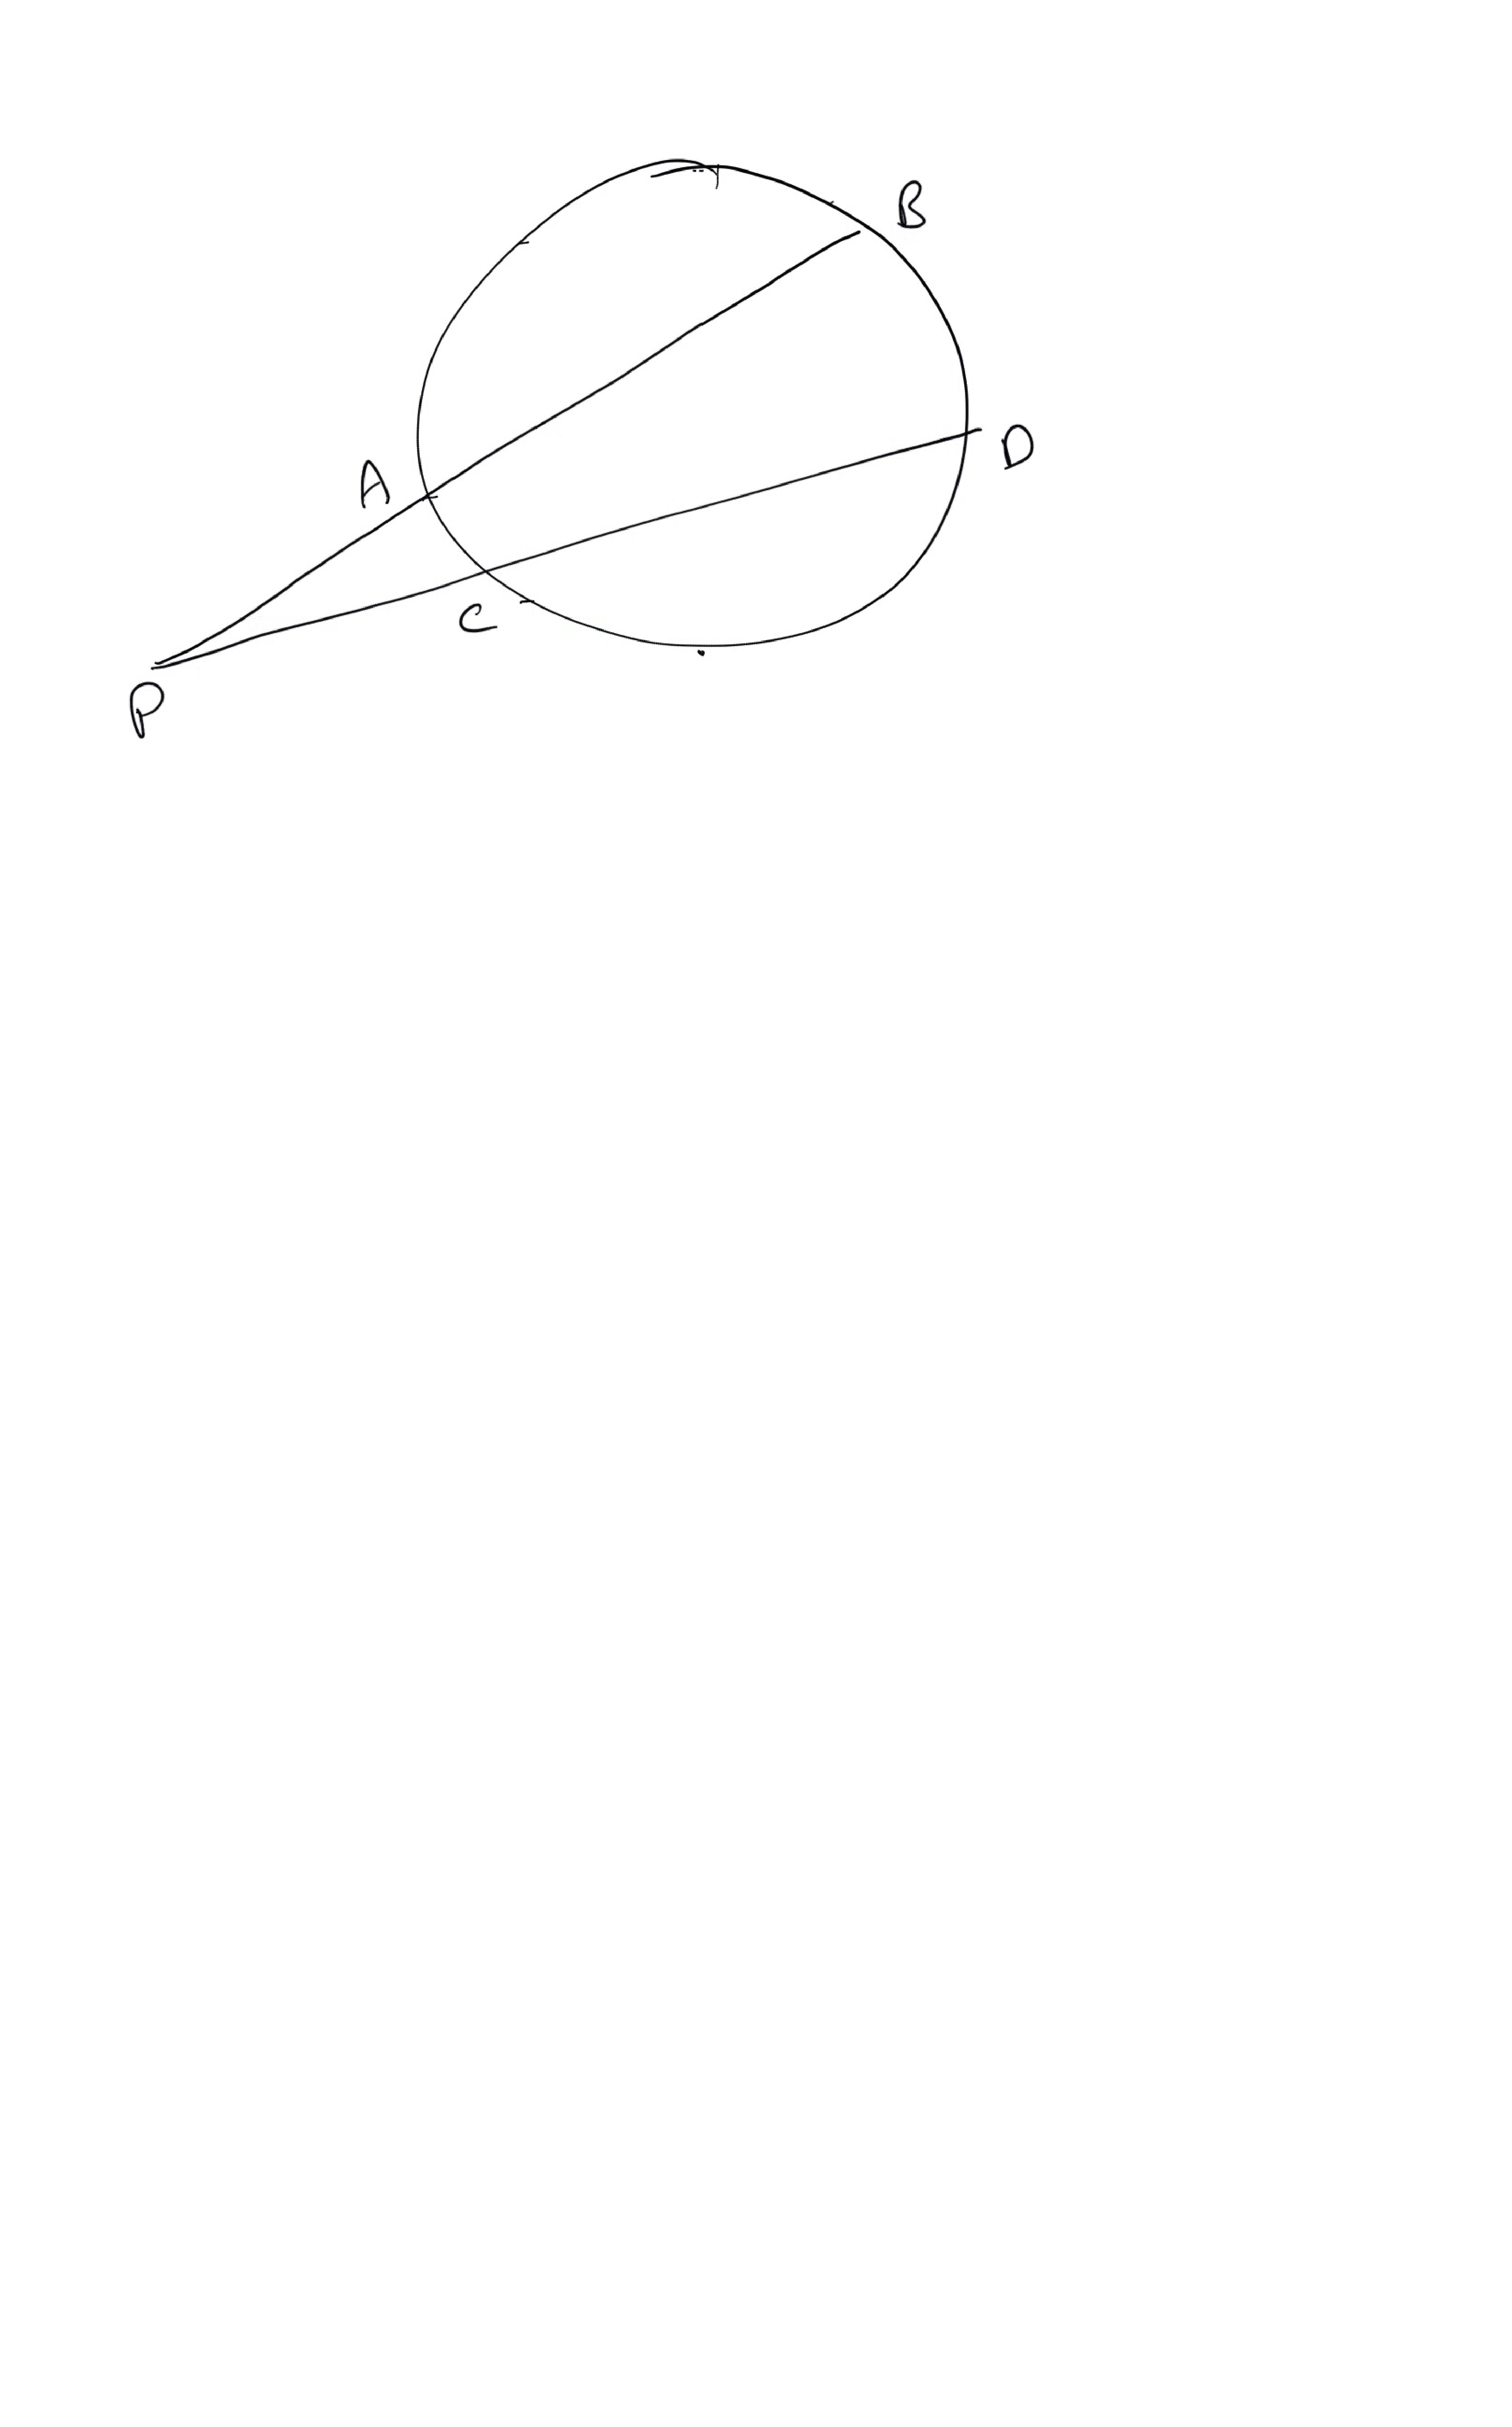
\includegraphics[width=\columnwidth]{./figs/ch4_chord_tangent_prod}
		\vspace*{-10cm}
	\end{center}
	\caption{$PA.PB = PC^2$.}
	\label{ch4_chord_tangent_prod}	
\end{figure}

\proof Draw a tangent and use the previous problem.
 




 
\subsection{Example}
\renewcommand{\theequation}{\theenumi}

\begin{enumerate}[label=\arabic*.,ref=\thesubsection.\theenumi]
\item In $\triangle ABC$,
\begin{equation}
\label{eq:linea}
\vec{A}=\myvec{1\\2}
\end{equation}
%
and the equations of the medians through $\vec{B}$ and $\vec{C}$
are respectively
\begin{align}
\label{eq:line_medb}
\myvec{1 & 1}\vec{x}&=5
\\
\myvec{1 & 0}\vec{x}&=4
\label{eq:line_medc}
\end{align}
%
Find the area of $\triangle ABC$.
\\
\solution The centroid $\vec{O}$ is the solution of \eqref{eq:line_medb},\eqref{eq:line_medc} and is obtained 
as the solution
of the matrix equation
\begin{align}
\myvec{1 & 1 \\1 & 0}\vec{x}&=\myvec{5 \\ 4}
\label{eq:line_matrix}
\end{align}
%
which can be solved using the augmented matrix as follows.
\begin{align}
\myvec{1 & 1 & 5\\1 & 0 & 4} \leftrightarrow \myvec{1 & 1 & 5\\0 & 1 & 1}\leftrightarrow  \myvec{1 & 0 & 4\\0 & 
1 & 1}
\end{align}
Thus,
\begin{equation}
\label{eq:lineo}
\vec{O}=\myvec{4\\1}
\end{equation}
% 
Let  $AD$ be the median through $\vec{A}$. Then,
\begin{align}
\frac{\vec{A}+\vec{B}+\vec{C}}{3}&= \vec{O}
\\
\implies \vec{B}+\vec{C}= 3\vec{O}-\vec{A} &= \myvec{11 \\ 1}
\label{eq:line_b+c}
\\
\implies \myvec{1 & 1}\vec{B}+\myvec{1 & 1}\vec{C}&=  \myvec{1 & 1}\myvec{11 \\ 1}
\label{eq:line_ctemp}
\end{align}
%
From \eqref{eq:line_medc} and \eqref{eq:line_ctemp},
\begin{align}
 \myvec{1 & 1}\vec{B} &= 5 
\\
\implies 5+\myvec{1 & 1}\vec{C}&=  12
\\
\implies \myvec{1 & 1}\vec{C}&=  7
\label{eq:line_ctemp2}
\end{align}
From \eqref{eq:line_ctemp2} and \eqref{eq:line_medc}, $\vec{C}$ can be obtained by solving 
\begin{align}
\myvec{1 & 1 \\1 & 0}\vec{C}&=\myvec{7 \\ 4}
\label{eq:line_cmatrix}
\end{align}
using the augmented matrix as
\begin{align}
\myvec{1 & 1 & 7\\1 & 0 & 4} &\leftrightarrow \myvec{1 & 1 & 7\\0 & 1 & 3}\leftrightarrow \myvec{1 & 0 & 4\\0 & 
1 & 3}
\\
\implies \vec{C}&=\myvec{4\\3}
\end{align}
%
From \eqref{eq:line_b+c},
\begin{align}
\vec{B}&=\myvec{11\\1}-\myvec{4\\3}
=\myvec{7\\-2}
\end{align}
%
Thus,
\begin{align}
\frac{1}{2}
\begin{vmatrix}
\vec{A} & \vec{B} &\vec{C}
\\
1 & 1 & 1
\end{vmatrix}
=
\frac{1}{2}
\begin{vmatrix}
1 & 7 & 4\\2 & -2 & 3 \\ 1 & 1 & 1
\end{vmatrix} = 9
\end{align}
\item Summarize all the above computations through a Python script and plot $\triangle ABC$.
\\
\solution
\begin{lstlisting}
https://github.com/gadepall/school/raw/master/linalg/2D/manual/codes/triang.py
\end{lstlisting}
\begin{figure}
\centering
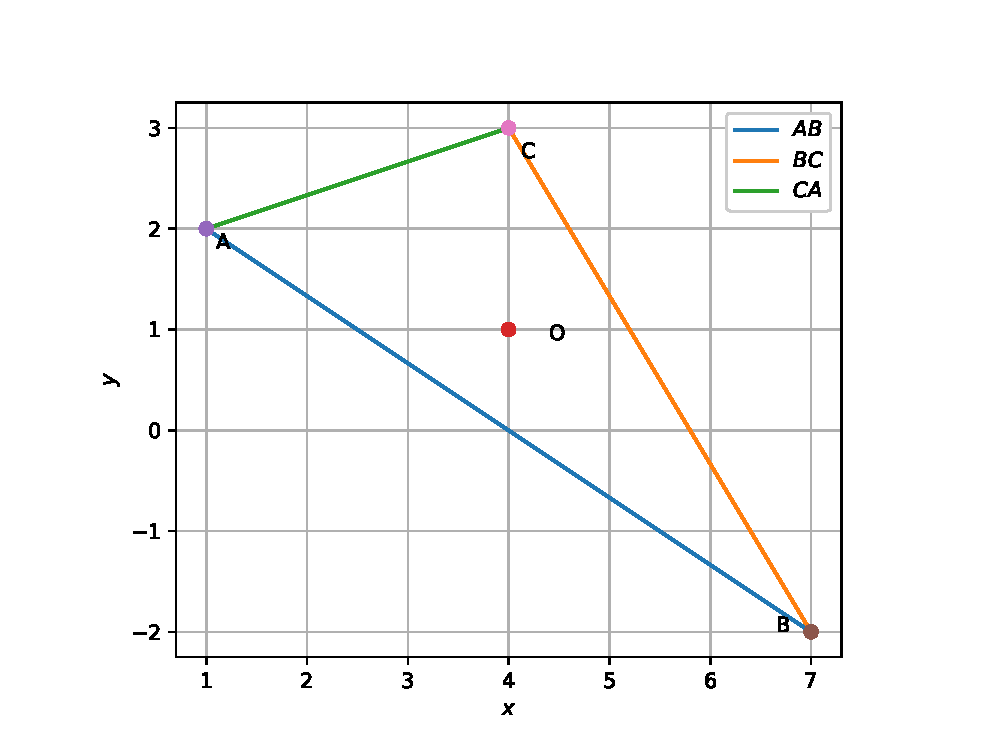
\includegraphics[width=\columnwidth]{./line/figs/triangle.eps}
\caption{}
\label{fig:triangle}
\end{figure}


%\numberwithin{equation}{enumi}

%\renewcommand{\theequation}{\theenumi}
\end{enumerate}
.
 
\subsection{Programming}
\renewcommand{\theequation}{\theenumi}

\begin{enumerate}[label=\arabic*.,ref=\thesubsection.\theenumi]
\numberwithin{equation}{enumi}
\item
Find the {\em orthocentre} of  $\triangle ABC$.
\\
\solution The following code finds the required point using \eqref{eq:alt_ap} and \eqref{eq:alt_bq}
.
\begin{lstlisting}
codes/2d/orthocentre.py
\end{lstlisting}

\item Find $\vec{P}$, the foot of the altitude from $\vec{A}$ upon BC.
%
\\
\solution 
\begin{lstlisting}
codes/2d/alt_foot.py
\end{lstlisting}
\item Find $\vec{Q}$ and $\vec{R}$.
\item Draw $AP, BQ$ and $CR$ and verify that they meet at a point 
$\vec{H}$.  
\\
\solution The following code plots the altitudes in Fig. \ref{fig:alt_triangle}
\begin{lstlisting}
codes/2d/alt_draw.py
\end{lstlisting}
\begin{figure}
\centering
\includegraphics[width=\columnwidth]{./line/figs/alt_triangle.eps}
\caption{}
\label{fig:alt_triangle}
\end{figure}
\item
Find the coordinates of $\vec{D}, \vec{E}$ and $\vec{F}$ of the mid points of $AB, BC$ and $CA$ respectively 
for  $\Delta ABC$. 
\item
Find the equations of $AD,BE$ and $CF$. 
%
\item
\label{prob:median}
Find the point of intersection of $AD$ and $CF$.
\item
Verify that $\vec{O}$ is the point of intersection of $BE,CF$ as 
well.
%as
\item
Graphically show that the medians of $\Delta ABC$ meet at the centroid.
\end{enumerate}

 
\subsection{Solved Problems}
%\documentclass[journal,12pt,twocolumn]{IEEEtran}
%\usepackage{setspace}
%\usepackage{gensymb}
%\usepackage{caption}
%%\usepackage{multirow}
%%\usepackage{multicolumn}
%%\usepackage{subcaption}
%%\doublespacing
%\singlespacing
%\usepackage{csvsimple}
%\usepackage{amsmath}
%\usepackage{multicol}
%%\usepackage{enumerate}
%\usepackage{amssymb}
%%\usepackage{graphicx}
%\usepackage{newfloat}
%%\usepackage{syntax}
%\usepackage{listings}
%\usepackage{iithtlc}
%\usepackage{color}
%\usepackage{tikz}
%\usetikzlibrary{shapes,arrows}
%
%
%
%%\usepackage{graphicx}
%%\usepackage{amssymb}
%%\usepackage{relsize}
%%\usepackage[cmex10]{amsmath}
%%\usepackage{mathtools}
%%\usepackage{amsthm}
%%\interdisplaylinepenalty=2500
%%\savesymbol{iint}
%%\usepackage{txfonts}
%%\restoresymbol{TXF}{iint}
%%\usepackage{wasysym}
%\usepackage{amsthm}
%\usepackage{mathrsfs}
%\usepackage{txfonts}
%\usepackage{stfloats}
%\usepackage{cite}
%\usepackage{cases}
%\usepackage{mathtools}
%\usepackage{caption}
%\usepackage{enumerate}	
%\usepackage{enumitem}
%\usepackage{amsmath}
%%\usepackage{xtab}
%\usepackage{longtable}
%\usepackage{multirow}
%%\usepackage{algorithm}
%%\usepackage{algpseudocode}
%\usepackage{enumitem}
%\usepackage{mathtools}
%\usepackage{hyperref}
%%\usepackage[framemethod=tikz]{mdframed}
%\usepackage{listings}
%    %\usepackage[latin1]{inputenc}                                 %%
%    \usepackage{color}                                            %%
%    \usepackage{array}                                            %%
%    \usepackage{longtable}                                        %%
%    \usepackage{calc}                                             %%
%    \usepackage{multirow}                                         %%
%    \usepackage{hhline}                                           %%
%    \usepackage{ifthen}                                           %%
%  %optionally (for landscape tables embedded in another document): %%
%    \usepackage{lscape}     
%
%
%\usepackage{url}
%\def\UrlBreaks{\do\/\do-}
%
%
%%\usepackage{stmaryrd}
%
%
%%\usepackage{wasysym}
%%\newcounter{MYtempeqncnt}
%\DeclareMathOperator*{\Res}{Res}
%%\renewcommand{\baselinestretch}{2}
%\renewcommand\thesection{\arabic{section}}
%\renewcommand\thesubsection{\thesection.\arabic{subsection}}
%\renewcommand\thesubsubsection{\thesubsection.\arabic{subsubsection}}
%
%\renewcommand\thesectiondis{\arabic{section}}
%\renewcommand\thesubsectiondis{\thesectiondis.\arabic{subsection}}
%\renewcommand\thesubsubsectiondis{\thesubsectiondis.\arabic{subsubsection}}
%
%% correct bad hyphenation here
%\hyphenation{op-tical net-works semi-conduc-tor}
%
%%\lstset{
%%language=C,
%%frame=single, 
%%breaklines=true
%%}
%
%%\lstset{
%	%%basicstyle=\small\ttfamily\bfseries,
%	%%numberstyle=\small\ttfamily,
%	%language=Octave,
%	%backgroundcolor=\color{white},
%	%%frame=single,
%	%%keywordstyle=\bfseries,
%	%%breaklines=true,
%	%%showstringspaces=false,
%	%%xleftmargin=-10mm,
%	%%aboveskip=-1mm,
%	%%belowskip=0mm
%%}
%
%%\surroundwithmdframed[width=\columnwidth]{lstlisting}
%\def\inputGnumericTable{}                                 %%
%\lstset{
%%language=C,
%frame=single, 
%breaklines=true,
%columns=fullflexible
%}
% 
%
%\begin{document}
%%
%\tikzstyle{block} = [rectangle, draw,
%    text width=3em, text centered, minimum height=3em]
%\tikzstyle{sum} = [draw, circle, node distance=3cm]
%\tikzstyle{input} = [coordinate]
%\tikzstyle{output} = [coordinate]
%\tikzstyle{pinstyle} = [pin edge={to-,thin,black}]
%
%\theoremstyle{definition}
%\newtheorem{theorem}{Theorem}[section]
%\newtheorem{problem}{Problem}
%\newtheorem{proposition}{Proposition}[section]
%\newtheorem{lemma}{Lemma}[section]
%\newtheorem{corollary}[theorem]{Corollary}
%\newtheorem{example}{Example}[section]
%\newtheorem{definition}{Definition}[section]
%%\newtheorem{algorithm}{Algorithm}[section]
%%\newtheorem{cor}{Corollary}
%\newcommand{\BEQA}{\begin{eqnarray}}
%\newcommand{\EEQA}{\end{eqnarray}}
%\newcommand{\define}{\stackrel{\triangle}{=}}
%
%\bibliographystyle{IEEEtran}
%%\bibliographystyle{ieeetr}
%
%\providecommand{\nCr}[2]{\,^{#1}C_{#2}} % nCr
%\providecommand{\nPr}[2]{\,^{#1}P_{#2}} % nPr
%\providecommand{\mbf}{\mathbf}
%\providecommand{\pr}[1]{\ensuremath{\Pr\left(#1\right)}}
%\providecommand{\qfunc}[1]{\ensuremath{Q\left(#1\right)}}
%\providecommand{\sbrak}[1]{\ensuremath{{}\left[#1\right]}}
%\providecommand{\lsbrak}[1]{\ensuremath{{}\left[#1\right.}}
%\providecommand{\rsbrak}[1]{\ensuremath{{}\left.#1\right]}}
%\providecommand{\brak}[1]{\ensuremath{\left(#1\right)}}
%\providecommand{\lbrak}[1]{\ensuremath{\left(#1\right.}}
%\providecommand{\rbrak}[1]{\ensuremath{\left.#1\right)}}
%\providecommand{\cbrak}[1]{\ensuremath{\left\{#1\right\}}}
%\providecommand{\lcbrak}[1]{\ensuremath{\left\{#1\right.}}
%\providecommand{\rcbrak}[1]{\ensuremath{\left.#1\right\}}}
%\theoremstyle{remark}
%\newtheorem{rem}{Remark}
%\newcommand{\sgn}{\mathop{\mathrm{sgn}}}
%\providecommand{\abs}[1]{\left\vert#1\right\vert}
%\providecommand{\res}[1]{\Res\displaylimits_{#1}} 
%\providecommand{\norm}[1]{\lVert#1\rVert}
%\providecommand{\mtx}[1]{\mathbf{#1}}
%\providecommand{\mean}[1]{E\left[ #1 \right]}
%\providecommand{\fourier}{\overset{\mathcal{F}}{ \rightleftharpoons}}
%%\providecommand{\hilbert}{\overset{\mathcal{H}}{ \rightleftharpoons}}
%\providecommand{\system}{\overset{\mathcal{H}}{ \longleftrightarrow}}
%	%\newcommand{\solution}[2]{\textbf{Solution:}{#1}}
%\newcommand{\solution}{\noindent \textbf{Solution: }}
%\newcommand{\myvec}[1]{\ensuremath{\begin{pmatrix}#1\end{pmatrix}}}
%\providecommand{\dec}[2]{\ensuremath{\overset{#1}{\underset{#2}{\gtrless}}}}
%\DeclarePairedDelimiter{\ceil}{\lceil}{\rceil}
%%\numberwithin{equation}{section}
%%\numberwithin{problem}{subsection}
%%\numberwithin{definition}{subsection}
%\makeatletter
%\@addtoreset{figure}{section}
%\makeatother
%
%\let\StandardTheFigure\thefigure
%%\renewcommand{\thefigure}{\theproblem.\arabic{figure}}
%\renewcommand{\thefigure}{\thesection}
%
%
%%\numberwithin{figure}{subsection}
%
%%\numberwithin{equation}{subsection}
%%\numberwithin{equation}{section}
%%\numberwithin{equation}{problem}
%%\numberwithin{problem}{subsection}
%\numberwithin{problem}{section}
%%%\numberwithin{definition}{subsection}
%%\makeatletter
%%\@addtoreset{figure}{problem}
%%\makeatother
%\makeatletter
%\@addtoreset{table}{section}
%\makeatother
%
%\let\StandardTheFigure\thefigure
%\let\StandardTheTable\thetable
%\let\vec\mathbf
%%%\renewcommand{\thefigure}{\theproblem.\arabic{figure}}
%%\renewcommand{\thefigure}{\theproblem}
%
%%%\numberwithin{figure}{section}
%
%%%\numberwithin{figure}{subsection}
%
%
%
%\def\putbox#1#2#3{\makebox[0in][l]{\makebox[#1][l]{}\raisebox{\baselineskip}[0in][0in]{\raisebox{#2}[0in][0in]{#3}}}}
%     \def\rightbox#1{\makebox[0in][r]{#1}}
%     \def\centbox#1{\makebox[0in]{#1}}
%     \def\topbox#1{\raisebox{-\baselineskip}[0in][0in]{#1}}
%     \def\midbox#1{\raisebox{-0.5\baselineskip}[0in][0in]{#1}}
%
%\vspace{3cm}
%
%\title{ 
%	\logo{
%The Straight Line and Linearity
%	}
%}
%
%\author{ G V V Sharma$^{*}$% <-this % stops a space
%	\thanks{*The author is with the Department
%		of Electrical Engineering, Indian Institute of Technology, Hyderabad
%		502285 India e-mail:  gadepall@iith.ac.in. All content in this manual is released under GNU GPL.  Free and open source.}
%	
%}	
%
%\maketitle
%
%%\tableofcontents
%
%\bigskip
%
%\renewcommand{\thefigure}{\theenumi}
%\renewcommand{\thetable}{\theenumi}
%
%
%\begin{abstract}
%	Solved problems from JEE mains papers related to 2D lines in coordinate geometry are 
%available in this document.  These problems are solved using linear algebra/matrix analysis.
%\end{abstract}
%\begin{enumerate}[label=\arabic*]
%\numberwithin{equation}{enumi}

\renewcommand{\theequation}{\theenumi}

\begin{enumerate}[label=\arabic*.,ref=\thesubsection.\theenumi]
\item A straight line through the origin   $\vec{O}$ meets the lines
\begin{align} 
\label{eq:line_1}
\myvec{4 & 3}\vec{x} &= 10
\\
\myvec{8 & 6}\vec{x} +5&= 0
\end{align} 
%
at $\vec{A}$ and $\vec{B}$ respectively.  Find the ratio in which  $\vec{O}$ divides $AB$.
\\
\solution Let 
\begin{align} 
\vec{n} =\myvec{4 \\ 3}
\end{align} 
%
Then \eqref{eq:line_1} can be expressed as
\begin{align} 
\label{eq:line_1_normal}
\vec{n}^T\vec{x} &= 10
\\
2\vec{n}^T\vec{x} &= -5
\end{align} 
%
and since $\vec{A}, \vec{B}$ satisfy \eqref{eq:line_1_normal} respectively,
\begin{align} 
\label{eq:line_1_normal_a}
\vec{n}^T\vec{A} &= 10
\\
2\vec{n}^T\vec{B} &= -5
\label{eq:line_1_normal_b}
\end{align} 
%
Let  $\vec{O}$ divide the segment $AB$ in the ratio $k:1$. Then
\begin{align} 
\label{eq:line_1_section}
\vec{O}=\frac{k\vec{B} +\vec{A} }{k+1}
\end{align} 
%
\begin{align} 
%\label{eq:line_1_section}
\because \vec{O}&= \vec{0},
\\
\vec{A} &=-k\vec{B}
\end{align} 
%
Substituting in \eqref{eq:line_1_normal_a}, and simplifying, 
\begin{align} 
\label{eq:line_1_normal_subs_a}
\vec{n}^T\vec{B} &= \frac{10}{-k}
\\
\vec{n}^T\vec{B} &= \frac{-5}{2}
%\label{eq:line_1_normal_b}
\end{align} 
resulting in 
\begin{align} 
\frac{10}{-k} = \frac{-5}{2} \implies k = 4
\end{align} 
\item The 
point 
\begin{equation} 
\vec{P}=\myvec{2\\ 1} 
\end{equation} 
is translated parallel to the line 
\begin{equation} 
\label{line_2}
L: \myvec{1 & -1}\vec{x} = 4 
\end{equation} 
% 
by $d =2\sqrt{3}$ units.  If the new point $\vec{Q}$ lies in the third 
quadrant, then find the equation of the line passing through $\vec{Q}$ and perpendicular to $L$. 
\\
\solution From \eqref{line_2}, the direction vector of $L$ is
\begin{equation} 
\label{line_2_m}
\vec{m} = \myvec{1 \\ 1} 
\end{equation} 
Thus, 
\begin{equation} 
\label{line_2_q}
\vec{Q}= \vec{P} + \lambda \vec{m}
\end{equation} 
However, 
\begin{align} 
PQ &= d
\\
\implies\norm{\vec{P}- \vec{Q}} &= \abs{\lambda}\norm{\vec{m}} =  d
\\
\implies \lambda &= \pm \frac{d}{\norm{\vec{m}}} = \pm \sqrt{6}
\label{line_2_lam}
\end{align} 
%
\begin{align} 
\because \norm{\vec{m}} = \sqrt{\vec{m}^T\vec{m}}= \sqrt{2}
\end{align} 
%
from \eqref{line_2_m}.  Since $\vec{Q}$ lies in the third quadrant, from \eqref{line_2_q} and \eqref{line_2_lam},
\begin{align} 
\vec{Q} = \myvec{2\\ 1}  -  \sqrt{6}\myvec{1\\ 1} =  \myvec{2-\sqrt{6}\\ 1-\sqrt{6}}
\end{align} 
%
The equation of the desired line is then obtained as 
\begin{align} 
\label{line_2_final}
\vec{m}^T\brak{\vec{x}-\vec{Q}}&= 0
\\
 \myvec{1 & 1}\vec{x} &= 3 -2\sqrt{6}
\end{align} 
\item Two sides of a rhombus are along the lines
\begin{align}
\label{eq:lines_4_ab}
AB: \myvec{1 & -1}\vec{x} + 1 &=0
\\
AD: \myvec{7 & -1}\vec{x} -5 &=0.
\label{eq:lines_4_ad}
\end{align}
%
If its diagonals intersect at 
\begin{equation}
\vec{P}=\myvec{-1\\ -2},
\label{eq:lines_4_p}
\end{equation}
find its vertices.
\\
\solution From \eqref{eq:lines_4_ab} and \eqref{eq:lines_4_ad},
\begin{align}
\myvec{1 & -1 \\ 7 & -1}\vec{A}  &=\myvec{-1 \\ 5}
\end{align}
%
By row reducing the augmented matrix
\begin{align}
\myvec{1 & -1 & -1\\ 7 & -1 & 5}  &\leftrightarrow \myvec{1 & -1 & -1\\ 0 & 6 & 12}\leftrightarrow \myvec{1 & -1 & -1\\ 0 & 1 & 2}
\nonumber \\
&\leftrightarrow \myvec{1 & 0 & 1\\ 0 & 1 & 2} \implies \vec{A}=\myvec{1\\ 2},
\label{eq:lines_4_a}
\end{align}
%
Since diagonals of a rhombus bisect each other, 
\begin{align}
\vec{P}&=\frac{\vec{A}+\vec{C}}{2}
\nonumber \\
\vec{C}&=2\vec{P}-\vec{A} = \myvec{-3\\-6}
\label{eq:lines_4_c}
\end{align}
%
\begin{align}
\because AD \parallel BC,&
\nonumber \\
BC: \myvec{7 & -1}\brak{\vec{x}-\vec{C}} &=0
\nonumber \\
\implies \myvec{7 & -1}\vec{x} &=-15
\label{eq:lines_4_bc}
\end{align}
%
From \eqref{eq:lines_4_ab} and \eqref{eq:lines_4_bc},
\begin{align}
 \myvec{7 & -1 \\ 1 & -1}\vec{B} &=\myvec{-15 \\ -1}
\end{align}
resulting in the augmented matrix
\begin{align}
& \myvec{7 & -1 & -15\\ 1 & -1 & -1} 
\leftrightarrow
 \myvec{7 & -1 & -15\\ 0 & 3 & -4} 
\nonumber \\
&\leftrightarrow
 \myvec{3 & 0 & -7\\ 0 & 3 & -4} \implies \vec{B} = -\frac{1}{3}\myvec{7\\4}
\end{align}
\begin{align}
\because AB \parallel CD,&
\nonumber \\
CD: \myvec{1 & -1}\brak{\vec{x}-\vec{C}} &=0
\nonumber \\
\implies \myvec{1 & -1}\vec{x} &=3
\label{eq:lines_4_cd}
\end{align}
%
From \eqref{eq:lines_4_ad} and \eqref{eq:lines_4_cd},
\begin{align}
 \myvec{7 & -1 \\ 1 & -1}\vec{D} &=\myvec{5 \\ 3}
\end{align}
resulting in the augmented matrix
\begin{align}
& \myvec{7 & -1 & 5\\ 1 & -1 & 3} 
\leftrightarrow
 \myvec{7 & -1 & 5\\ 0 & 3 & -8} 
\nonumber \\
&\leftrightarrow
 \myvec{3 & 0 & 1\\ 0 & 3 & -8} \implies \vec{D} = \frac{1}{3}\myvec{1\\-8}
\end{align}

%From \eqref{eq:lines_4_p} and \eqref{eq:lines_4_a}
%\begin{align}
%AP =\norm{\vec{A}-\vec{P}} = 2\sqrt{5} =d (say)
%\end{align}
%%
%The direction vector of $AP$ is 
%\begin{align}
%\vec{m} &=\vec{A}-\vec{P} = 2\myvec{1\\ 2}
%\\
%\implies \norm{\vec{m}} &= 2\sqrt{5}
%\end{align}
%Since the direction of $AP$ is the same as $AC$,
%\begin{align}
%\vec{C} &=\vec{P}-d\frac{\vec{m}}{\norm{\vec{m}}} 
%\nonumber \\
%&= -\myvec{1\\ 2}- 2\myvec{1\\ 2} = \myvec{-3\\ -6}
%\end{align}
%
%Let $\vec{n}\perp\vec{m}$. Then 
%\begin{align}
%\vec{n} &=\myvec{2\\ -1}
%\end{align}
%%
%and 
%\begin{align}
%\vec{B,D} &=\vec{P}\pm d\frac{\vec{n}}{\norm{\vec{n}}} 
%\nonumber \\
%&=-\myvec{1\\ 2}\pm 2\myvec{2\\ -1} = \myvec{5\\ 0}, \myvec{-3\\ 4}
%\end{align}

\item Let $k$ be an integer such that the triangle with vertices
\begin{equation}
\label{eq:lines_5}
\vec{A} = \myvec{k\\-3k},
\vec{B} =\myvec{5\\k},
\vec{C} =\myvec{-k\\2}
\end{equation}
has area 28.  Find the orthocentre of this triangle.
%
\\
\solution Let $\vec{m}_1$ be the direction vector of $BC$.  Then,
\begin{align}
\label{eq:lines_5_m1}
\vec{m}_1 = \myvec{5+k\\k-2},
\end{align}
%
If $AD$ be an altitude, its equation can be obtained as
\begin{align}
\label{eq:lines_5_m1a}
\vec{m}_1^{T}\brak{\vec{x}-\vec{A}} = 0
\end{align}
%
Similarly, considering the side $AC$  the equation of the altitude $BE$ is
\begin{align}
\label{eq:lines_5_m2b}
\vec{m}_2^{T}\brak{\vec{x}-\vec{B}} = 0
\end{align}
%
where 
\begin{align}
\label{eq:lines_5_m2}
\vec{m}_2 = \myvec{2k\\-2-3k},
\end{align}
The orthocentre is obtained by solving \eqref{eq:lines_5_m1a}
and \eqref{eq:lines_5_m2b} using the matrix equation
\begin{align}
\myvec{\vec{m}_1\\ \vec{m}_2}^T \vec{x} 
= \myvec{ \vec{m}_1^T\vec{A}\\ \vec{m}_2^T
\vec{B}}
\end{align}
%
which can be expressed using \eqref{eq:lines_5_m1}, 
\eqref{eq:lines_5_m2}, 
\eqref{eq:lines_5_m1a} and 
\eqref{eq:lines_5_m2b}
as 
\begin{align}
\myvec{5+k & k-2 \\2k & -2-3k} \vec{x} 
&= \myvec{ k^2+5k+6k-3k^2\\ 10k-2k-3k^2}
\nonumber \\
&= k\myvec{ 11-4k\\ 8-3k}
\label{eq:lines_5_h}
\end{align}
%
%The solution to the above is 
%\begin{align}
%\vec{x} &= k\myvec{5+k & k-2 \\2k & -2-3k}^{-1} \myvec{ 11-4k\\ 8-3k}
%\nonumber \\
%&= \frac{k}{-3k^2-17k-10-2k^2+4k}
%\nonumber \\
%&\times \myvec{-2-3k & -k+2 \\-2k & 5+k} \myvec{ 11-4k\\ 8-3k}
%\nonumber \\
%&= \frac{k}{5k^2+13k+10}
%\nonumber \\
%&\times \myvec{2+3k & k-2 \\2k & -5-k} \myvec{ 11-4k\\ 8-3k}
%\nonumber \\
%&= \frac{k}{5k^2+13k+10}
%\nonumber \\
%&\times 
%\myvec{ 22-12k^2-8k+33k -3k^2+6k+8k-16 \\ 22k-8k^2-40+15k-8k+3k^2}
%\nonumber \\
%&= \frac{k}{5k^2+13k+10}
%\myvec{ 6+39k-15k^2 \\ -40+29k-5k^2}
%\end{align}
From \eqref{eq:lines_5}, using the expression for the area of triangle,
\begin{align}
\begin{vmatrix}
k & 5 & -k\\-3k & k & 2 \\ 1 & 1 & 1
\end{vmatrix} = 56
\nonumber \\
\implies
\begin{vmatrix}
k & 5-k & -2k\\-3k & 4k & 2+3k \\ 1 & 0 & 0
\end{vmatrix} = 56
\end{align}
%
resulting in
\begin{align}
\brak{5-k}
\brak{2+3k}+8k^2=56
\\
\implies 5k^2+13k-46 = 0
\\
\text{or, } k = 2, -\frac{23}{5}
\end{align}
Substituting the above in \eqref{eq:lines_5_h} and solving yields the orthocentre.
\item If an equilateral triangle, having centroid at the origin, has a side along the line
\begin{equation}
\label{eq:lines_6_ab}
\myvec{1 & 1}\vec{x} = 2,
\end{equation}
then find the area of this triangle. Also draw the equilateral triangle and two medians to verify your results.
\\
\solution Let the vertices be $\vec{A},\vec{B},\vec{C}$. From the given information, 
\begin{align}
\frac{\vec{A}+\vec{B}+\vec{C}}{3} &= \vec{0}
\nonumber \\
\implies 
\vec{A}+\vec{B}+\vec{C} = \vec{0}
\label{eq:lines_6_abc}
\end{align}
%
If $AB$ be the line in \eqref{eq:lines_6_ab},
%\begin{equation}
%\label{eq:lines_6_nab}
%\myvec{1 & 1}\brak{\vec{A}-\vec{B}} = 0
%\end{equation}
%%
%Thus, the direction vector of $AB$ is 
%\begin{align}
%\label{eq:lines_6_mab}
%\vec{m} = \myvec{1 \\ -1}
%\end{align}
the equation of 
$CF$, where 
\begin{align}
\vec{F} = \frac{\vec{A}+\vec{B}}{2} 
\end{align}
is 
%
\begin{align}
\label{eq:lines_6_cf}
\myvec{1 & -1}\vec{x} = 0
\end{align}
since $CF$ passes through the origin and $CF\perp AB$. From \eqref{eq:lines_6_ab}
and \eqref{eq:lines_6_cf},
\begin{align}
\label{eq:lines_6_fmat}
\myvec{1 & 1 \\1 & -1}\vec{F} = \myvec{2 \\ 0}
\end{align}
%
Forming the augmented matrix, 
\begin{align}
\myvec{1 & 1 &2 \\1 & -1 & 0} &\leftrightarrow \myvec{1 & 1 &2 \\0 & 2 & 2} \leftrightarrow \myvec{1 & 1 &2 \\0 & 1 & 1} 
\nonumber \\
&\leftrightarrow \myvec{1 & 0 &1 \\0 & 1 & 1} \implies \vec{F} = \myvec{1 \\ 1}
\label{eq:lines_6_f}
\end{align}
From \eqref{eq:lines_6_abc},
\begin{align}
\vec{C}=-\brak{\vec{A}+\vec{B}}=-2\vec{F} = -2\myvec{1 \\ 1}
\label{eq:lines_6_c}
\end{align}
after substituting from \eqref{eq:lines_6_f}.  Thus, 
\begin{align}
CF &= \norm{\vec{C}-\vec{F}} = 3\sqrt{2} 
\\
\implies AB &=  CF\frac{2}{\sqrt{3}} = 2\sqrt{6}
\label{eq:lines_6_cflen}
\end{align}
and the area of the triangle is 
\begin{align}
\frac{1}{2} AB \times CF = 6\sqrt{3}
\end{align}


\item A square, of each side 2, lies above the $x$-axis and has one vertex at the origin.  If one of the sides 
passing through the origin makes an angle $30^{\degree}$ with the positive direction of the $x$-axis, then 
find the 
sum of the $x$-coordinates of the vertices of the square.
\\
\solution Consider the square $ABCD$ with $\vec{A} = \vec{0}, AB = 2$ such that $\vec{B}$ and $\vec{D}$ lie on the $x$ and $y$-axis respectively. Then 
\begin{align}
\vec{A}+\vec{B}+\vec{C}+\vec{D} = 4\myvec{1 \\ 1}
\label{eq:lines_7_abcdsum}
\end{align}
%
Multiplying \eqref{eq:lines_7_abcdsum} with the rotation matrix 
\begin{align}
\label{eq:lines_7_t}
\vec{T} = \myvec{\cos \theta & -\sin \theta \\ \sin \theta & \cos \theta},
\end{align}
\begin{align}
\vec{T}\brak{\vec{A}+\vec{B}+\vec{C}+\vec{D}} &= 4\myvec{\cos \theta & -\sin \theta \\ \sin \theta & \cos \theta}\myvec{1 \\ 1}
\nonumber \\
&= 4\myvec{\cos \theta  -\sin \theta \\ \cos \theta + \sin \theta}
%\nonumber \\
\end{align}
\begin{multline}
\implies \myvec{1 & 0}\vec{T}\brak{\vec{A}+\vec{B}+\vec{C}+\vec{D}} 
\\
= 4\brak{\cos \theta  -\sin \theta}
= 2\brak{\sqrt{3}-1}
\end{multline}
%
for $\theta = 30^{\degree}$. Draw the square with sides on the axis as well as the rotated square in the same graph to verify your result.


%\item Find the locus of the point of intersection of the lines
%\begin{align}
%\myvec{\sqrt{2} & -1 }\vec{x} + 4 \sqrt{2}k &= 0
%\\
%\myvec{\sqrt{2}k & k }\vec{x} - 4 \sqrt{2} &= 0
%\end{align}

\end{enumerate}
%\section{Trigonometry}
%\begin{enumerate}[label=\thesection.\arabic*
%,ref=\thesection.\theenumi]
%
%\item In $\triangle PQR$, which is not right angled, let
%\begin{align}
%PQ = r, QR = p, RP = q
%\end{align}
%%
%The median $RS$ and the altitude $PE$  intersect at $\vec{O}$. $p =\sqrt{3}, q = 1$ and the radius of the circumcircle  of $\triangle PQR = k = 1$.  
%\item Find  $RS$
%\\
%\solution Using the sine formula,
%\begin{align}
%\frac{p}{\sin P}=\frac{q}{\sin Q} = 2k
%\\
%\implies \sin P = \frac{\sqrt{3}}{2}, \sin Q = \frac{1}{2}
%\end{align}
%If $\angle R \ne \frac{\pi}{2}$, the only possible solution is 
%\begin{align}
%\angle P = \frac{2\pi}{3},
%\angle Q = \frac{\pi}{6},
%\angle R = \frac{\pi}{6}
%\end{align}
%%
%$\because \angle Q = \angle R, q = r = 1$.  The given information is shown in Fig. \ref{fig:2019_8}
%\begin{figure}
%\centering
%\includegraphics[width=\columnwidth]{./line/figs/2019_8.eps}
%\caption{}
%\label{fig:2019_8}
%\end{figure}
%%
%Using the cosine formula, 
%\begin{align}
%RS &= \sqrt{q^2+\brak{\frac{r}{2}}^2-qr\cos P}
%\\
%&= \sqrt{1+\frac{1}{4}+\frac{1}{2}} = \sqrt{\frac{7}{2}}
%\end{align}
%\item Find $OE$.
%\\
%\solution 
%Using Baudhayana's theorem,
%\begin{align}
%OE  &= \sqrt{OR^2 - ER^2}
%\\
%&= \sqrt{\brak{\frac{2RS}{3}}^2 - \brak{\frac{p}{2}}^2} 
%\\
%&= \sqrt{\frac{7}{9}-\frac{3}{4}} = \frac{1 }{6}
%\end{align}
%%
%\item Find the area of $\triangle SOE$
%\\
%\solution
%$\because$ $PE$ and $RS$ are medians, 
%\begin{align}
%\text{ar}\brak{\triangle SOE }&= \frac{1}{4}\text{ar}\brak{\triangle POR},
%\\
%\text{ar}\brak{\triangle POR }&=  \frac{2}{3}\text{ar}\brak{\triangle PER},
%\\
%\text{ar}\brak{\triangle PER }&=  \frac{1}{2}\text{ar}\brak{\triangle PQR},
%\\
%\implies \text{ar}\brak{\triangle SOE} &= \frac{1}{12}\text{ar}\brak{\triangle PQR}
%&= \frac{\sqrt{3}}{24}
%\end{align}
%
%\item Find the radius of the incircle of $\triangle PQR $.
%%
%\\
%\solution
%I is the incentre in Fig. \ref{fig:2019_8}.  The radius of the incircle is 
%\begin{align}
%\frac{p}{2\cos\frac{Q}{2}} &= \frac{p}{\sqrt{2\brak{1+\cos Q}}}
%\\ &= \sqrt{\frac{3}{1+\sqrt{3}}}
%\end{align}
%%
%\item Repeat all the above exercises using vector algebra and plot Fig. \ref{fig:2019_8}.
%\end{enumerate}
%
%\end{document}
 
\subsection{JEE Exercises}
\renewcommand{\theequation}{\theenumi}
\begin{enumerate}[label=\arabic*.,ref=\thesubsection.\theenumi]
\numberwithin{equation}{enumi}

    \item Find the area enclosed within the curve $\abs{x} + \abs{y} = 1 $.
    \item Find the equation of the line about which y=$10^x$ is the reflection of y=$\log_{10}x$.

    \item If $3a+2b+4c=0$, find the intersection of the  set of lines 
  \begin{align} 
    \myvec{a & b}\vec{x} + c &= 0.
    \end{align}
    \item Given the points $A=\myvec{0 \\ 4}$ and $B=\myvec{0 \\ -4}$, find the equation of the locus of the point $P=\myvec{x \\ y}$ such that $\abs{AP-BP} $=6.
    \item If a,b and c are in A.P, show that  the straight line 
\begin{align} 
    \myvec{a & b}\vec{x} + c &= 0
    \end{align}
will always pass through a fixed point and find its coordinates.
    \item Find the quadrant in which the orthocentre of the triangle formed by the lines 
\begin{align} 
    \myvec{1 & 1}\vec{x}  &= 1
\\
    \myvec{2 & 3}\vec{x}  &= 6
\\
    \myvec{4 & -1}\vec{x} + 4 &= 0
    \end{align} lies.
    \item Let the algebraic sum of the perpendicular distances from the points $\myvec{2 \\ 0}$,  $\myvec{0 \\ 2}$ and $\myvec{1 \\ 1}$ to a variable straight line be zero.  Show that  the line passes through a fixed point and find its  coordinates. 
    \item The vertices of a triangle are $\vec{A}=\myvec{-1 \\ -7},\vec{B}=\myvec{5 \\ 1}$ and $\vec{C}=\myvec{1 \\ 4}$. Find the equation of the bisector of $\angle ABC$.
    \item Verify if the straight line 
\begin{align} 
    \myvec{5 & 4}\vec{x} &= 0
    \end{align} passes through the point of intersection of the straight lines \begin{align} 
    \myvec{1 & 2}\vec{x} - 10 &= 0
    \end{align} and \begin{align} 
    \myvec{2 & 1}\vec{x} + 5 &= 0
    \end{align}
    \item Do the lines \begin{align} 
    \myvec{2 & 3}\vec{x} + 19 &= 0
    \end{align} and \begin{align} 
    \myvec{9 & 6}\vec{x} - 17 &= 0
    \end{align} cut the coordinate axes in concyclic points?
    \item The points $\myvec{-a\\b}$,\myvec{0\\0},\myvec{a\\b} and \myvec{a^2\\ab} are:
    \begin{enumerate}
    \item  Collinear
    \item  Vertices of a parallelogram
    \item  Vertices of a rectangle
    \item  None of these
    \end{enumerate}
    \item The point $\myvec{4 \\ 1}$ undergoes the following three transformations successively
    (i) Reflection about the line \begin{align} 
    \myvec{-1 & 1}\vec{x} &= 0
    \end{align}
    (ii)Translation through a distance 2 units along the positive direction of x-axis
    (iii) Rotation through an angle $\frac{\pi}{4}$ about the origin in counter clockwise direction.
    Find  the final position of the point.
\item The straight lines \begin{align} 
    \myvec{1 & 1}\vec{x} &= 0
\\
    \myvec{3 & 1}\vec{x} - 4 &= 0
\\
    \myvec{1 & 3}\vec{x} - 4 &= 0
    \end{align}form a triangle which is
    \begin{enumerate}
     \item isosceles
     \item equilateral
     \item right angled
     \item none of these
     \end{enumerate}
    \item If $\vec{P}=\myvec{1\\0}$, $\vec{Q}=\myvec{-1\\0}$ and $\vec{R}=\myvec{2\\0}$ are three given points, then the locus of the point $\vec{S}$ satisfying the relation $SQ^2+SR^2=2SP^2$, is
    \begin{enumerate}
     \item  a straight line parallel to X-axis
     \item a circle passing through the origin
     \item a circle with centre at the origin
     \item  a straight line parallel to Y-axis.
     \end{enumerate}
    \item Line L has intercepts a and b on the coordinate axes.When the axes are rotated through a given angle, keeping the origin fixed, the same line L has intercepts p and q, then
    \begin{enumerate}
     \item  $a^2+b^2=p^2+q^2$
     \item  $\frac{1}{a^2}+\frac{1}{b^2}=\frac{1}{p^2}+\frac{1}{q^2}$
     \item  $a^2+p^2=b^2+q^2$
     \item  $\frac{1}{a^2}+\frac{1}{p^2}=\frac{1}{b^2}+\frac{1}{q^2}$
     \end{enumerate}
    \item If the sum of the distances of a point from two perpendicular lines in a plane is 1, then its locus is
    \begin{enumerate}
     \item  Square
     \item  Circle
     \item  Straight line
     \item  Two intersecting lines
     \end{enumerate}
    \item The locus of a variable point whose distances from $\myvec{-2\\0}$ is $\frac{2}{3}$ times its distance from the line $x=-\frac{9}{2}$ is
    \begin{enumerate}
     \item  Ellipse
     \item  Parabola
     \item  Hyperbola
     \item  None of these
    \end{enumerate}
    \item The equations of a pair of opposite sides of a parallelogram are  
\begin{align} 
x^2-5x+6 = 0
\\
y^2-6y+5 = 0
\end{align}
Find  the equations of its diagonals. 
    \item Find the orthocentre of the triangle formed by the lines 
\begin{align}
    \vec {x}^T\myvec{0 & 1 \\ 1 & 0} \vec{x} &=0
    \end{align} 
and 
\begin{align}
\myvec{1 & 1} \vec x =1
    \end{align} 
    \item Let PQR be an isosceles triangle, right angled at  $\vec{P}=\myvec{2\\1}$. If the equation of the line QR is \begin{align}\myvec{2 & 1}\vec{x} = 3, \end{align} then find the equation representing the pair of lines PQ and PR is
    \item If $x_1,x_2,x_3$ as well as $y_1,y_2,y_3$ are in G.P with the same common ratio, then the points\myvec{x_1\\y_1},\myvec{x_2\\y_2} and \myvec{x_3\\y_3}
    \begin{enumerate}
     \item  lie on a straight line
     \item  lie on a ellipse
    \item  lie on a circle
    \item  are the vertices of a triangle
    \end{enumerate}
    \item Let PS be the median of the triangle with vertices $\vec{P}=\myvec{2\\2}, \vec{Q}=\myvec{6\\-1}$ and $\vec{R}=\myvec{7\\3}$. Find the equation of the line passing through $\myvec{1\\-1}$ and parallel to PS.
    \item Find the incentre of the triangle with vertices $\myvec{1\\\sqrt{3}},\myvec{0\\0}$ and $\myvec{2\\0}$. 
    \item The number of integer values of $m$, for which the x coordinate of the point of intersection of the lines \myvec{3\\4}$\vec {x}=9$ and \myvec{-m\\1}$\vec {x} -1=0$  is also an integer, is
    \begin{enumerate}
     \item  2
     \item  0
     \item  4
     \item  1
     \end{enumerate}
    \item Find the area of the parallelogram formed by the lines \myvec{-m\\1}$\vec {x}$=0, \myvec{-m\\1}$\vec {x}$+1=0 ,\myvec{-n\\1}$\vec {x}$=0 and \myvec{-n\\1}$\vec {x}$+ 1 =0.
    \item Let $0 <\alpha< \frac{\pi}{2}$  be a fixed angle. If
    $\vec{P}=\myvec{\cos\theta \\ \sin \theta}$ and $\vec{Q}=\myvec{\cos\brak{\alpha-\theta}\\ \sin\brak{\alpha-\theta}}$
    then the $\vec{Q}$ is obtained from $\vec{ P}$ by
    \begin{enumerate}
     \item  clockwise rotation around origin through an angle$\alpha$
     \item  anticlockwise rotation around origin through an angle$\alpha$
     \item  reflection in the line through origin with slope $\tan \alpha$
     \item  reflection in the line through origin with slope $\tan \frac{\alpha}{2}$
     \end{enumerate}
    \item Let $\vec{P}=\myvec{-1\\0} \vec{Q}=\myvec{0\\0}$ and $\vec{R}=\myvec{3\\3\sqrt{3}}$ be three points. Then find the equation of the bisector of the angle PQR.
    \item A straight line through the origin $\vec{O}$ meets the parallel lines \begin{align} \myvec{4 & 2} \vec {x} &= 9\end{align} and \begin{align} \myvec{2 & 1} \vec {x} + 6 &= 0\end{align} at points $\vec{P}$ and $\vec{Q}$ respectively. Find the ratio in which $\vec{O}$ divides the segment PQ. 
    \item The number of integral points (integral points means both the coordinate should be integer) exactly in the interior of the triangle with the vertices \myvec{0\\0} , \myvec{0\\21} and  \myvec{21\\0} is 
    \begin{enumerate}
     \item 133
     \item 190
     \item 233
     \item 105
     \end{enumerate}
    \item Find the orthocentre of a triangle with vertices   \myvec{0\\0},\myvec{3\\4},\myvec{4\\0} 
    \item Find the area of the triangle formed by the line \begin{align} \myvec{1 & 1} \vec {x} &= 3\end{align} and angle bisectors of the pair of straight lines \begin{align}\vec{x}^T \myvec{1 & 0 \\ 0 & -1} \vec {x} + \myvec{0 & 2} \vec {x} &= 1.\end{align}
    \item Let $\vec{O}= \myvec{0\\0}, \vec{P}=\myvec{3\\4}, \vec{Q}= \myvec{6\\0}$  be the vertices of the triangle OPQ. The point $\vec{R}$ inside the triangle OPQ is such that the triangles OPR,PQR, OQR are of equal area. Find the coordinates of $\vec{R}$.
    \item A straight line L through the point \myvec{3\\-2} is inclined at an angle of $60\degree$ to the line\begin{align} \myvec{\sqrt{3} & 1} \vec {x} &= 1.\end{align} If L also intersects the x-axis, then find the equation of L.
%

    \item Three lines \begin{align}\myvec{p & q} \vec {x} + r &= 0,\end{align} \begin{align}\myvec{q & r} \vec {x} + p &= 0\end{align} and \begin{align}\myvec{r & p} \vec {x} + q &= 0\end{align} are concurrent if
    \begin{enumerate}
     \item  $p+q+r=0$
     \item  $p^2+q^2+r^2=qr+rp+pq$
     \item  $p^3+q^3+r^3=3pqr$
     \item  none of these
     \end{enumerate}
    \item The points \myvec{0\\\frac{8}{3}},\myvec{1\\3} and \myvec{82\\30} are vertices of 
    \begin{enumerate}
     \item  an obtuse angled triangle
     \item  an acute angled triangle
     \item  a right angled triangle
     \item  none of these
     \end{enumerate}
    \item All points lying inside the triangle formed by the points \myvec{1\\3}, \myvec{5\\0} and \myvec{-1\\2} satisfy
    \begin{enumerate}
     \item  $\myvec{3 & 2} \vec {x} \geq 0$
     \item  $\myvec{2 & 1} \vec {x}-13\geq 0$
     \item  $\myvec{2 & -3} \vec {x}-12\leq 0$
     \item  $\myvec{-2 & 1} \vec {x} \geq 0$
     \item none of these
     \end{enumerate}
    \item A vector $\vec{a} = \myvec{2p \\ 1}$  with respect to a rectangular cartesian system. The system is rotated through a certain angle about the origin in the counter clockwise sense. If, with respect to the new system,  $\vec {a} = \myvec{p+1\\1}$, then
    \begin{enumerate}
     \item  p=0
     \item  p=1 or p=$-\frac{1}{3}$
     \item  p=-1 or p=$\frac{1}{3}$
     \item  p=1 or p=-1
     \item none of these
     \end{enumerate}
    \item If $\vec{P} = \myvec{1\\2}, \vec{Q} = \myvec{4\\6}, \vec{R} = \myvec{5\\7}$ and $\vec{S} = \myvec{a\\b}$ are the vertices of a parallelogram PQRS, find $a$ and $b$.
    \item The diagonals of a parallelogram PQRS are along the lines \begin{align}\myvec{1 & 3} \vec {x} &= 4\end{align} and \begin{align}\myvec{6 & -2} \vec {x} &= 7\end{align}. Then PQRS must be a
    \begin{enumerate}
     \item  rectangle
     \item  square
     \item  cyclic quadrilateral
     \item  rhombus
     \end{enumerate}
    \item If the vertices $\vec{P}, \vec{Q} , \vec{R}$ of a triangle PQR are rational points, which of the following points of the triangle PQR is (are) always rational point(s)?
    \begin{enumerate}
     \item  centroid
     \item  incentre
     \item  circumcentre
     \item  orthocentre
     \end{enumerate}
    \item Let $L_1$ be a straight line passing through the origin and $L_2$ be the straight line \begin{align}\myvec{1 & 1} \vec {x} &= 1.\end{align} If the intercepts made by the circle  \begin{align}\vec{x}^T\vec{x} + \myvec{-1 & 3} \vec {x} &= 0\end{align} on $L_1$ and $L_2$ are equal, then which of the following equations can represent $L_1$?
    \begin{enumerate}
     \item  $\myvec{1 & 1} \vec {x} = 0$
     \item  $\myvec{1 & -1} \vec {x} = 0$
     \item  $\myvec{1 & 7} \vec {x} = 0$
     \item  $\myvec{1 & -7} \vec {x} = 0$
     \end{enumerate}
    \item For $a > b > c > 0$, the distance between $\myvec{1\\1}$ and the point of intersection of the lines $\myvec{a & b}\vec {x}+c=0$ and $\myvec{b & a} \vec {x}+c=0$ is less than 2$\sqrt2$. Then 
    \begin{enumerate}
     \item  a+b-c\textgreater 0
     \item  a-b+c\textless 0
     \item  a-b+c\textgreater 0
     \item  a+b-c\textless 0
    \end{enumerate}
    \item  A straight line segment of length $l$, moves with its ends on two mutually perpendicular lines. Find the locus of the points which divides the line segment in the ratio 1:2.
    \item The area of triangle is 5. Two of its vertices are $\vec{A} = \myvec{2\\1}, \vec{B} = \myvec{3\\-2}$. The third vertex $\vec{C}$ lies on $\myvec{-1 & 1}\vec {x} = 3$. Find $\vec{C}$.
    \item One side of a rectangle lies along the line \begin{align}\myvec{4 & 7} \vec {x} + 5 &= 0.\end{align} Two of its vertices are \myvec{-3\\1} and \myvec{1\\1}. Find the equations of the other three sides.
    \item  Two vertices of a triangle are \myvec{5\\-1} and \myvec{2\\-3}. If  the orthocentre of the triangle is the origin, find the coordinates of the third point.
     \item  Find the equation of the line which bisects the obtuse angle between the lines \begin{align}\myvec{1 & -2} \vec {x} + 4 &= 0\end{align} and \begin{align}\myvec{4 & -3} \vec {x} -2 &= 0.\end{align}
    \item A straight line L is perpendicular to the line \begin{align}\myvec{5 & -1} \vec {x} &= 1.\end{align} The area of the triangle formed by the line L and the coordinate axes is 5. Find the equation of the line L.
    \item The end $\vec{A},\vec{B}$ of a straight line segment of constant length c slide upon the fixed rectangular axis OX,OY respectively. If the rectangle OAPB be completed, then show that the locus of the foot of the perpendicular drawn from $\vec{P}$ to AB is $x^{2/3}+y^{2/3}=c^{2/3}$.
    \item The vertices of a triangle are $\myvec{a t_1t_2 \\ a(t_1+t_2)},\myvec{a t_2t_3 \\ a(t_2+t_3)},\myvec{a t_3t_1\\ a(t_3+t_1)}$. Find the orthocentre of the triangle.
    \item The coordinates of $\vec{A}, \vec{B}, \vec{C}$ are $\myvec{6\\3},\myvec{-3\\5},\myvec{4\\-2}$ respectively, and $\vec{P}$ is any point $\vec{x}$. Show that the ratio of the area of the triangles $\triangle PBC$ and $\triangle ABC$ is $ \frac{\abs{\myvec{1 & 1}\vec {x}-2}}{7}$
    \item Two equal sides of an isosceles triangles are given by the equations \begin{align}\myvec{7 & -1} \vec {x} + 3 &= 0 \end{align} and \begin{align}\myvec{1 & 1} \vec {x} - 3 &= 0 \end{align} and its third side passes through the point \myvec{1\\10}. Determine the equation of third side.
    \item One of the diameters of the circle circumscribing the rectangle ABCD is \begin{align}\myvec{-1 & 4} \vec {x}  &= 7. \end{align} If A and B are the points \myvec{-3\\4} and \myvec{5\\4} respectively, then find the area of the rectangle.
    \item Two sides of a rhombus ABCD are parallel to the lines \begin{align}\myvec{-1 & 1} \vec {x}  &= 2 \end{align} and \begin{align}\myvec{-7 & 1} \vec {x}  &= 3 \end{align}. If the diagonals of the rhombus intersect at the point \myvec{1 \\ 2} and  vertex $\vec{A}$ is on the y axis. Find possible coordinates of $\vec{A}$.
    \item Lines \begin{align}L_1\equiv\myvec{a & b} \vec {x} + c &= 0 \end{align} \begin{align}L_2\equiv\myvec{l & m} \vec {x} + n &= 0 \end{align} intersect at the point $\vec{P}$ and make an angle $\theta$ with each other. Find the equation of a line L different from $L_2$ which passes through $\vec{P}$ and makes the same angle $\theta$ with $L_1$.
    \item Let ABC be a traingle with AB=AC. If $\vec{D}$ is the mid point of BC, $\vec{E}$ is the foot of the perpendicular drawn from $\vec{D}$ to AC and $\vec{F}$ the mid-point of DE, Prove that AF perpendicular to BE.
    \item Straight lines\begin{align}\myvec{3 & 4} \vec {x}  &= 5 \end{align} and \begin{align}\myvec{4 & -3} \vec {x}  &= 15 \end{align} intersect at the point $\vec{A}$. Points $\vec{B}$ and $\vec{C}$ are chosen on these two lines such that AB=AC. Determine the possible equations of the lines BC passing through the point\myvec{1\\2}
    \item A line cuts the x-axis at $\vec{A}= \myvec{7\\0}$ and the y-axis at $\vec{B}=\myvec{0\\-5}$. A variable line PQ is draw perpendicular to AB cutting the x-axis in $\vec{P}$ and the y-axis in $\vec{Q}$. If AQ and BP intersect at $\vec{R}$, find the locus of $\vec{R}$.
    \item Find the equation of the line passing through the point \myvec{2\\3} and making an intercept of  length 2 units between the lines $\myvec{2 & 1}\vec {x}$=3 and $\myvec{2 & 1} \vec {x}$=5.
%\includegraphics[scale=1.5]{sample}
    \item Show that all chords of the curve  \begin{align}\vec{x}^T\myvec{3 & 0 \\ 0 & -1} \vec {x} + \myvec{-2 & 4} \vec {x} &= 0 \end{align} which subtend a right angle at the origin, pass through a fixed point. Find the coordinates of the point.
    \item Determine all values of $\alpha$ for which the point $\myvec{\alpha\\ \alpha^2}$ lies inside the triangle formed by the lines 
    \begin{align}\myvec{2 & 3} \vec {x} -1 &= 0  \\ \myvec{1 & 2} \vec {x} -3 &= 0 \\ \myvec{5 & -6} \vec {x} -1 &= 0 \end{align}
    \item The tangent at a point $\vec{P}_1$ (other than the origin) on the curve 
    \begin{align}y = x^3 \end{align} meets the curve again at $\vec{P}_2$. The tangent at $\vec{P}_2$ meets the curve at $\vec{P}_3$ and so on. Show that the abscissae of $\vec{P}_1,\vec{P}_2,\vec{P}_3 \dots \vec{P}_n$, form a G.P. Also find the ratio $\frac{\text{area}(\triangle P_1,P_2,P_3)}{\text{area}(\triangle P_2,P_3,P_4)}$.
    \item A line through $\vec{A}=\myvec{-5\\-4}$ meets the line $\myvec{1 & 3}\vec {x}+2=0,\myvec{2 &1} \vec {x}$ +4=0 and $\myvec{1 & -1}\vec {x}$ -5=0 at the points $\vec{B},\vec{C}$ and $\vec{D}$ respectively. If
\begin{align}
\brak{\frac{15}{AB}}^2+\brak{\frac{10}{AC}}^2 = \brak{\frac{6}{AD}}^2,
\end{align}
find the equation of the line.
    \item A rectangle PQRS has its side PQ parallel to the line \begin{align}\myvec{-m & 1} \vec {x}  &= 0 \end{align} and vertices $\vec{P},\vec{Q}$ and $\vec{S}$ on the lines 
\begin{align}
\myvec{0 & 1} \vec {x}  &= a 
\\
\myvec{1 & 0} \vec {x}  &= b 
\\
\myvec{1 & 0} \vec {x}  &= -b 
\end{align} respectively. Find the locus of vertex $\vec{R}$.
    \item Using coordinate geometry, prove that the three altitudes of any triangle are concurrent.
    \item For points $\vec{P}=\myvec{x_1\\y_1}$ and $\vec{Q}=\myvec{x_2\\y_2}$ of the coordinate plane, a new distance $d(\vec{P},\vec{Q})=\vert x_1-x_2\vert+ \vert y_1-y_2\vert$. Let $\vec{O}=\myvec{0\\0}$ and $\vec{A}=\myvec{3\\2}$. Prove that the set of points in the first quadrant which are equidistant (with respect to the new distance) from $\vec{O}$ and $\vec{A}$ consists of the union of a line segment of finite length and an infinite ray. Sketch this set in a labelled diagram.
    \item Let ABC and PQR be any two triangles in the same plane. Assume that the perpendiculars from the points $\vec{A},\vec{B},\vec{C}$ to the sides QR,RP,PQ respectively are concurrent. Using vector methods or otherwise, prove that the perpendiculars from $\vec{P},\vec{Q},\vec{R}$ to BC,CA,AB respectively are also concurrent.
    \item Let a,b,c be real numbers with $a^2+b^2+c^2=1$. show that the equation
    \begin{align}\mydet{\myvec{a & -b}\vec {x} - c & \myvec{b & a}\vec {x} & \myvec{c & 0}\vec {x} + a \\ \myvec{b & a}\vec {x} &  \myvec{-a & b}\vec {x} - c & \myvec{0 & c}\vec {x} + b \\ \myvec{c & 0}\vec {x} + a & \myvec{0 & c}\vec {x} + b & \myvec{-a & -b}\vec {x} + c} = 0 \end{align} represents a straight line.
    \item A straight line L through the origin meets the line and \begin{align}\myvec{1 & 1} \vec {x} &= 3 \end{align} at $\vec{P}$ and $\vec{Q}$ respectively. Through $\vec{P}$,  straight lines $L_1$ and $L_2$ are drawn parallel to \begin{align}\myvec{2 & -1} \vec {x} &= 5 \\ \myvec{3 & 1} \vec {x}  &= 5 \end{align} respectively. Lines $L_1$ and $L_2$ intersect at that the locus of $\vec{R}$, as L varies, is a straight line.
    \item A straight line L with negative slope passes through point \myvec{8\\2} and cuts the positive coordinates are $\vec{P}$ and $\vec{Q}$. Find the absolute minimum value of OP varies, where $\vec{O}$ is origin.
    \item The area of the triangle formed by the intersection of a line parallel to the x-axis and passing through $\vec{P}= \myvec{h\\k}$ with the lines 
\begin{align}
\myvec{1 & -1} \vec {x} &= 0 
\\
\myvec{1 & 1} \vec {x} &= 2 
\end{align} is 4$h^2$. Find the locus of the point.
    \item Lines 
\begin{align}L_1: \myvec{-1 & 1} \vec {x} &=0
\\
L_2: \myvec{2 & 1} \vec {x} &=0
\end{align} 
intersect the line 
\begin{align}
L_3: \myvec{0 & 1} \vec {x} + 2 &=0
\end{align} at $\vec{P}$ and $\vec{Q}$ respectively. 
The bisector of the acute angle between $L_1$ and $L_2$ intersects $L_3$ at $\vec{R}$.
\begin{enumerate}[label=Statement-\arabic*.,ref=\thesubsection.\theenumi]
\item The ratio PR:RQ equals 2$\sqrt2:\sqrt5$
\item In any triangle, the bisector of an angle divides the triangle into two similar triangles.
\end{enumerate}
\begin{enumerate}
    
     \item  Statement-1 is true, Statement-2 is true ; Statement-2 is not a correct explanation for Statement-1
     \item  Statement-1 is true, Statement-2 is true ;  Statement-2 is not a correct explanation for Statement-1
     \item  Statement-1 is True,Statement False
     \item  Statement-1 is False,Statement True\\
\end{enumerate}


\item For a point $\vec{P}$ in the plane, let $d_1(\vec{P})$ and $d_2(\vec{P})$ be the distance of the point $\vec{P}$ from the lines 
\begin{align} 
\myvec{1 & -1} \vec {x} &=0
\\
\myvec{1 & 1} \vec {x} &=0
\end{align} 
respectively. 
Find the area of the region $R$ consisting of all points $\vec{P}$ lying in the first quadrant of the plane and satisfying 
\begin{align} 
2\leq d_1(\vec{P})+d_2(\vec{P}) \leq 4.
\end{align} 
    \item A triangle with vertices \myvec{4\\0},\myvec{-1\\-1} and \myvec{3\\5} is
    \begin{enumerate}
     \item  isosceles and right angled
     \item  isosceles but not right angled
     \item  right angled but not isosceles
     \item  neither right angled nor isosceles
     \end{enumerate}
    \item Find the locus of mid points of the portion between the axis of 
\begin{align}\myvec{\cos\alpha & \sin\alpha}\vec {x} &= 0\end{align} 
where p is constant
    \item If the pair of the lines \begin{align} \vec{x}^T\myvec{a & 2h \\ 0 & b} \vec {x} + 2\myvec{g & f}\vec {x} + c &=0\end{align}  intersects the y-axis then
    \begin{enumerate}
     \item  $2fgh=bg^2$+c$h^2$
     \item  $bg^2\neq c h^2$
     \item  $abc=2fgh$
     \item  none of these
     \end{enumerate}
    \item A pair of lines represented by \begin{align} \vec{x}^T\myvec{3a & 5 \\ 0 & (a^2-2)} \vec {x} &=0\end{align} are perpendicular to each other for
    \begin{enumerate}
     \item  two values of a 
     \item  $\forall$ a
     \item  for one value of a 
     \item  for no values of a 
     \end{enumerate}
    \item A square of side $ a$ lies above the x-axis and has one vertex at the origin. The side passing through the origin makes an angle $\alpha (0\textless\alpha\textless\pi$/4) with the positive direction of the x-axis. Find the equation of its diagonal not passing through the origin.
    \item If the pair of straight lines \begin{align}\vec{x}^T \myvec{1 & -2p \\ 0 & -1}\vec {x} &= 0\end{align} and \begin{align}\vec{x}^T \myvec{1 & -2q \\ 0 & -1}\vec {x} &= 0\end{align} be such that each pair bisects the angle between the other pair, then find the relation between $p$ and $q$.
    \item Find the locus of the centroid of the triangle whose vertices are \myvec{a \cos t\\a \sin t} , \myvec{b \sin t\\-b \cos t} and \myvec{1\\0}.
    \item If $x_1$,$x_2$,$x_3$ and $y_1$,$y_2$,$y_3$ are both in G.P. with the same common ratio, then the common points $\myvec{x_1\\y_1}, \myvec{x_2\\y_2}$ and $\myvec{x_3\\y_3}$
    \begin{enumerate}
     \item  are verices of a triangle
     \item  lie on a straight line
     \item  lie on a ellipse
     \item  lie on a circle
     \end{enumerate}
    \item If the equation of the locus of a point equidistant from the points $\myvec{a_1\\b_1}, \myvec{a_2\\b_2}$ is \begin{align}\myvec{a_1-b_2 & a_1-b_2}\vec {x} +c &= 0 \end{align} then find the value of c. 
    \item Let $\vec{A}=\myvec{2\\-3}$ and $\vec{B}=\myvec{-2\\3}$ be the vertices of a triangle ABC. If the centroid of the triangle moves on the line \begin{align}\myvec{2 & 3}\vec {x} &= 1 \end{align} then find the locus of the vertex $\vec{C}$.
    \item Find the equation of the straight line passing through the point \myvec{4\\3} and making intercepts on the coordinate axis whose sum is -1.
    \item If the sum of the slopes of the lines given by $\vec {x}^T \myvec{1 & -2c \\ 0 & -1} \vec {x} = 0$ is 4 times their product, then find  $c$.
    \item If one of the lines given by \begin{align}\vec {x}^T \myvec{6 & -1 \\ 0 & 4c} \vec {x} &= 0\end{align} is \begin{align}\myvec{ 3 & 4} \vec {x} &= 0\end{align} then find $c$.
    \item The line parallel to the x-axis and passing through the intersection of the lines \begin{align}\myvec{a & 2b} \vec {x} + 3b &= 0 \\ \myvec{b & -2a} \vec {x} - 3a &= 0, \end{align} where \myvec{a\\b}$\neq$\myvec{0\\0} is
    \begin{enumerate}
     \item  below the x-axis at a distance of 3/2 from it
     \item  below the x-axis at a distance of 2/3 from it
     \item  above the x-axis at a distance of 3/2 from it
     \item  above the x-axis at a distance of 2/3 from it
     \end{enumerate}
    \item If a vertex of a triangle is \myvec{1\\1} and the mid points of two sides through this vertex are \myvec{-1\\2} and \myvec{3\\2}, then find the centroid of the triangle.
    \item A straight line through the point $\vec{A} = \myvec{3\\4}$ is such that its intercepts between the axes is bisected at $\vec{A}$. Find its equation.
    \item If $\myvec{a\\a^2}$ falls inside the angle made by the lines \begin{align}\myvec{-1 & 2} \vec {x} &= 0,  \\ \myvec{-3 & 1} \vec {x} &= 0 \\ \myvec{1 & 0} \vec{x} &> 0,\end{align} then find the range of $a$. 
    \item Let $\vec{A}=\myvec{h\\k}, \vec{B}=\myvec{1\\1}$ and  $\vec{C}=\myvec{2\\1}$ be the vertices of a right angled triangle with AC has its hypotenuse. If the area of the triangle is 1 sq.unit, then find the range of $k$.
    \item Let $\vec{P}=\myvec{-1\\0}, \vec{Q}=\myvec{0\\0}$ and $\vec{R}=\myvec{3\\\sqrt3}$ be three points. Find the equation of the bisector of the angle PQR. 
    \item If one of the lines of \begin{align}\vec{x}^T\myvec{-m & (1-m^2) \\ 0 & m} \vec {x} &= 0\end{align} is a bisector of the angle between the lines  \begin{align}\vec{x}^T\myvec{0 & 0 \\ 1 & 0} \vec {x} &= 0,\end{align} then find m.
    \item The perpendicular bisector of the line segment joining $\vec{P}=\myvec{1\\4}$ and $\vec{Q}=\myvec{k\\3}$ has y-intercept -4. Then a possible value of k is
    \begin{enumerate}
     \item  1 
     \item  2
     \item  -2
     \item  -4
     \end{enumerate}
    \item Find the shortest distance between the line \begin{align}\myvec{-1 & 1}\vec{x} &= 1\end{align} and the curve \begin{align}\vec{x}^T\myvec{0 & 0 \\ 0 & 1} \vec {x} + \myvec{-1 & 0} &= 0\end{align}.
    \item The lines \begin{align}\myvec{(p(p^2+1) & -1}\vec{x} + q &= 0\\ \myvec{(p^2+1)^2 & (p^2+1)}\vec{x} + 2q &= 0\end{align} are perpendicular to a common line for:
    \begin{enumerate}
     \item  exactly one values of p
     \item  exactly two values of p
     \item  more than two values of p
     \item  no value of p
     \end{enumerate}
    \item Three distinct points $\vec{A},\vec{B}$ and $\vec{C}$ are given in the two dimensional coordinates plane such that the ratio of the distance of any one of them from the point \myvec{1\\0} to the distance from the point \myvec{-1\\0} is equal to $\frac{1}{3}$. Find the circumcentre of the triangle ABC.
    \item The line L given by \begin{align}\myvec{1/5 & 1/b}\vec{x} &= 1\end{align}  passes through the point \myvec{13\\32}. The line K is parallel to L and has the equation \begin{align}\myvec{\frac{1}{c} & \frac{1}{3}}\vec{x} = 1\end{align}. Find the distance between L and K. 
    \item If the line \begin{align}\myvec{2 & 1}\vec{x} &= k\end{align} passes through the point which divides the line segment joining the points\myvec{1\\1} and \myvec{2\\4} in the ratio 3:2, then find $k$.
    \item A ray of light along \begin{align}\myvec{1 & \sqrt3}\vec{x} &= \sqrt3\end{align} gets reflected upon reaching the x-axis, then find the equation of the reflected ray. 
    \item Find the x coordinate of the incentre of the triangle that has the coordinates of the mid points of its sides as \myvec{0\\1},\myvec{1\\1} and \myvec{1\\0}
    \item Let PS be the median of the triangle with vertices $\vec{P}= \myvec{2\\2}, \vec{Q}=\myvec{6\\-1} $ and $\vec{R}=  \myvec{7\\3}$. Find the equation of the line passing through \myvec{1\\-1} and parallel to PS. 
    \item Let a,b,c and d be non zero numbers. If the point of  intersection of the lines $\myvec{4a & 2a}\vec{x} + c = 0$ and $\myvec{5b & 2b}\vec{x} + d = 0$ lies in the fourth quadrant and is equidistant from the two axes, then
    \begin{enumerate}
     \item  3bc-2ad=0
     \item  3bc+2ad=0
     \item  2bc-3ad=0
     \item  2bc+3ad=0\\
     \end{enumerate}
    \item The number of points, having both coordinates as integers, that lie in the interior of the triangle with vertices \myvec{0\\0},\myvec{0\\41} and\myvec{41\\0}. 
is:
    \begin{enumerate}
     \item  820 
     \item  780
     \item  901
     \item  861\\
     \end{enumerate}
    \item Two sides of a rhombus are along the lines, \myvec{1&-1} $\vec {x}$+1=0 and \myvec{7&-1}$\vec {x}$-5=0. If its diagonals intersect at \myvec{-1\\-2} then which one of the following is a vertex of the rhombus?
    \begin{enumerate}
     \item  \myvec{\frac{1}{3}\\\frac{8}{3}}
     \item  \myvec{\frac{10}{3}\\\frac{7}{3}}
     \item  \myvec{-3\\-9}
     \item  \myvec{-3\\-8}\\
     \end{enumerate}
    \item A straight the through a fixed point \myvec{2\\3} intersects the coordinate axes at distinct points $\vec{P}$ and $\vec{Q}$. If $\vec{O}$ is the origin and the rectangle OPRQ is completed, then find the locus of $\vec{R}$.
    \item Consider the set of all lines \myvec{p&q} $\vec {x}$+r=0 such that $3p+2q+4r=0$. Which one of the following statements is true?
    \begin{enumerate}
     \item  The lines are concurrent at the point \myvec{\frac{3}{4}\\\frac{1}{2}}
     \item  Each line passes through the origin
     \item  The lines are all parallel
     \item  The lines are not concurrent
     \end{enumerate}
    \item Find the slope of a line passing through $\vec{P} = \myvec{2\\3}$ and intersecting the line \myvec{1&1}
    $\vec {x}$=7 at a distance of 4 units from $\vec{P}$.
\end{enumerate}

%\end{document}
 
\section{The Circle}
\subsection{Definitions}
\renewcommand{\theequation}{\theenumi}
\begin{enumerate}[label=\arabic*.,ref=\thesubsection.\theenumi]
\item The points $\vec{O}=\myvec{0\\0},\vec{A}=\myvec{a_1\\a_2}$ are as shown in Fig. \ref{fig:line_homog}. 
Find the equation of  $OA$. 
\numberwithin{equation}{enumi}
\begin{figure}
\centering
\includegraphics[width=\columnwidth]{./figs/line_homog.eps}
\caption{}
\label{fig:line_homog}
\end{figure}
\\
\solution
Let $\vec{x}=\myvec{x_1\\x_2}$ be any point on $OA$.
Then, using similar triangles,
\begin{align}
\frac{x_2}{x_1} &= \frac{a_2}{a_1} = m
\\
\implies x_2 &=  m x_1
\end{align}
where $m$ is known as the slope of the line. Thus, the equation of the line is
\begin{align}
%\label{eq:homog}
\vec{x} = \myvec{x_1\\m x_1} = x_1 \myvec{1 \\ m} = x_1\vec{m}
\end{align}
In general, the above equation is written as
\begin{align}
\label{eq:homog}
\vec{x} = \lambda \vec{m},
\end{align}
%
where $\vec{m}$ is the direction vector of the line.

\item Find the equation of $AB$ in Fig. \ref{fig:line_nhomog}
\begin{figure}
\centering
\includegraphics[width=\columnwidth]{./figs/line_nhomog.eps}
\caption{}
\label{fig:line_nhomog}
\end{figure}
\\
\solution 
From Fig. \ref{fig:line_nhomog}, 
%
\begin{align}
\frac{x_2-a_2}{x_1-a_1} = \frac{b_2-a_2}{b_1-a_1} = m
\\
\implies x_2 = m x_1 + a_2-ma_1
\label{eq:line_shift}
\end{align}
%
From \eqref{eq:line_shift},
\begin{align}
\myvec{x_1 \\ x_2} &= 
\myvec{x_1 \\   m x_1 + a_2-ma_1
} 
\\
&=\vec{A} + \brak{x_1-a_1}  \myvec{1 \\ m}
\\
&=\vec{A} + \lambda  \vec{m}
\label{eq:nhomog}
\end{align}
\item {\em Translation:} If the line shifts from the origin by $\vec{A}$, \eqref{eq:nhomog} is obtained from \eqref{eq:homog} by adding $\vec{A}$.
\item Find the length of $\vec{A}$ in Fig. \ref{fig:line_homog}
\\
\solution Using Baudhayana's theorem, the length of the vector $\vec{A}$ is defined as
\begin{equation}
 \norm{\vec{A}} = OA = \sqrt{a_1^2 + a_2^2}
=\sqrt{\vec{A}^T\vec{A}}.
\end{equation}
%
Also, from \eqref{eq:homog}, 
\begin{equation}
\norm{\vec{A}} = \lambda \sqrt{1+m^2}
\end{equation}
%
Note that $\lambda$ is the variable that determines the length of $\vec{A}$, 
since $m$ is constant for all points on the line.
%
\item Find $\vec{A}-\vec{B}$.
\begin{figure}
\centering
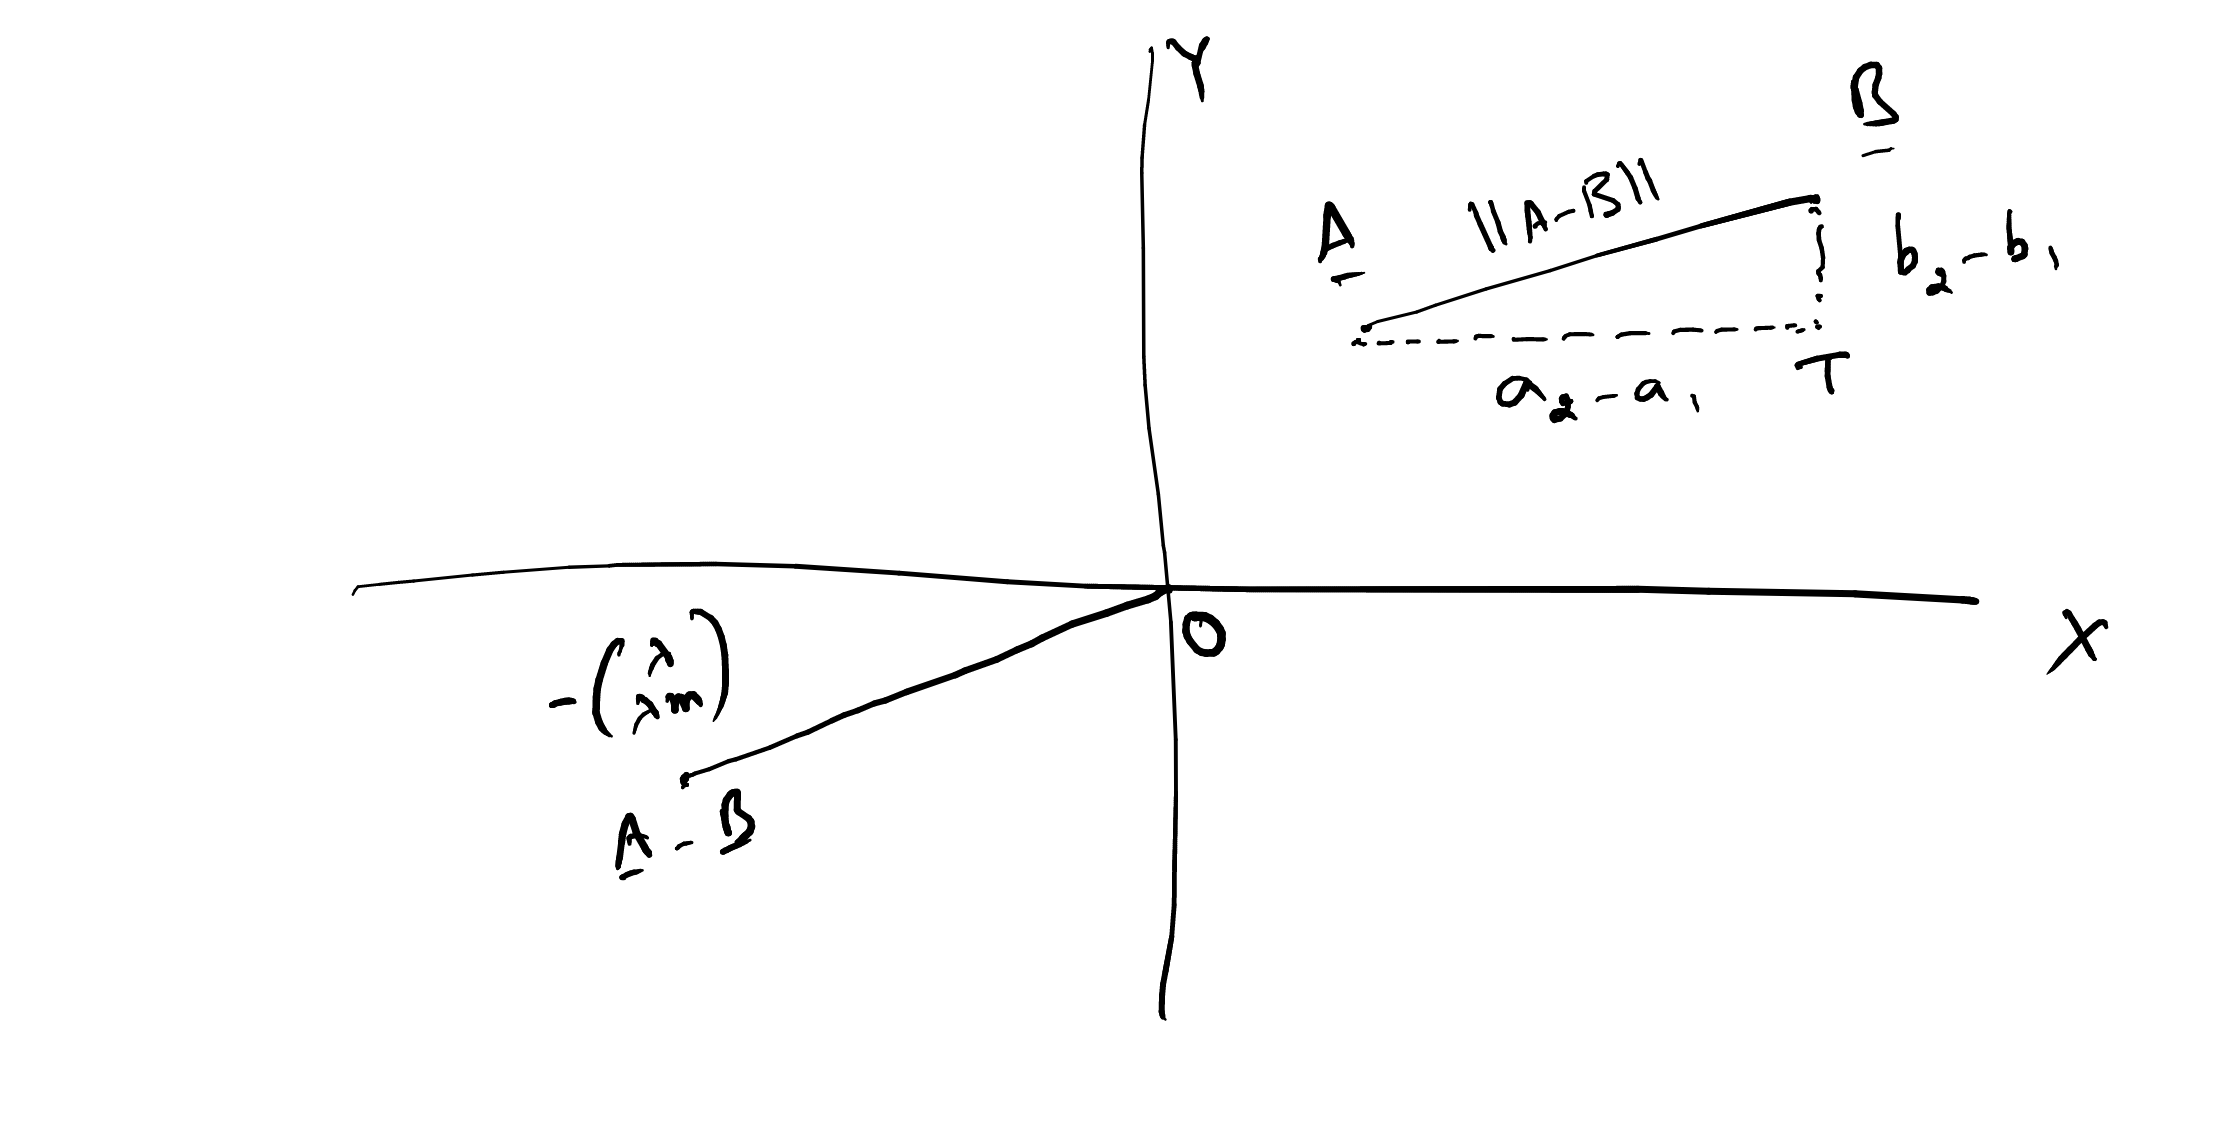
\includegraphics[width=\columnwidth]{./figs/ab.eps}
\caption{}
\label{fig:ab}
\end{figure}
%
\\
\solution See Fig. \ref{fig:ab}. From \eqref{eq:nhomog}, for some 
$\lambda$,
\begin{align}
\vec{B} &=\vec{A} + \lambda \myvec{1 \\ m}
\\
\implies \vec{A} - \vec{B} &= - \lambda \myvec{1 \\ m},
\end{align}
%
$\vec{A} - \vec{B}$ is marked in Fig. \ref{fig:ab}.
%
\item Show that $AB = \norm{\vec{A}-\vec{B}}$
\item Show that the equation of $AB$ is
\begin{align}
\label{eq:line_ab}
\vec{x} = \vec{A}+ \lambda\brak{\vec{B}-\vec{A}}
\end{align}
%
\item The {\em normal} to the vector $\vec{m}$ is defined as
\begin{align}
\label{eq:normal}
\vec{n}^T\vec{m} = 0
\end{align}
\begin{align}
\label{eq:normal_omat}
\vec{n} = \myvec{0 & 1\\ -1 & 0}\vec{m}
\end{align}
\item From \eqref{eq:line_ab}, the equation of a line can also be expressed as
\begin{align}
\label{eq:line_ab_normal}
\vec{n}^T\vec{x} &= \vec{n}^T\vec{A}+ \lambda\vec{n}^T\brak{\vec{B}-\vec{A}}
\\
\implies \vec{n}^T\vec{x} &=c
\label{eq:line_normal}
\end{align}
\item The unit vectors on the $x$ and $y$ axis are defined as
\begin{align}
\label{eq:line_unit}
\vec{e}_1 &=\myvec{1\\0}, 
\\
\vec{e}_2 &=\myvec{0\\1}
\end{align}
\item If $a$ be the {\em intercept} of the line 
\begin{align}
\label{eq:line_intercept}
\vec{n}^T\vec{x} &=c
\end{align}
on the $x-$axis, then $\myvec{a\\0}$  is a point on the line.  Thus, 
\begin{align}
%\label{eq:line_intercept}
\vec{n}^T\myvec{a\\0} &=c
\\
\implies a &= \frac{c}{\vec{n}^T\vec{e}_1}
\end{align}
%
\renewcommand{\theequation}{\theenumi}
%
\item The {\em rotation matrix} is defined as
\begin{align}
\vec{Q} = \myvec{\cos \theta & -\sin \theta\\ \sin \theta & \cos \theta}
\end{align}
%
where $\theta$ is anti-clockwise.
\item 
\begin{align}
\vec{Q}^T\vec{Q} = \myvec{1 & 0 \\ 0 & 1} = \vec{I}
\end{align}
%
where $\vec{I}$ is the {\em identity matrix}. The rotation matrix $\vec{Q}$ is also an {\em orthogonal matrix}.

\numberwithin{equation}{enumi}
%
\item Find the equation of  line $L$ in Fig. \ref{fig:line_dist}.
\\
\solution The equation of the $x-$axis is
\begin{align}
\vec{x} =\lambda \vec{e}_1
\end{align}
Translation by $p$ units along the $y-$axis results in 
\begin{align}
L_0: \quad \vec{x} = \lambda \vec{e}_1 + p \vec{e}_2 
\end{align}
Rotation by $90\degree-\alpha$ in the anti-clockwise direction yields
\begin{align}
L: \quad \vec{x} &= \vec{Q}\cbrak{\lambda \vec{e}_1 + p \vec{e}_2 }
\\
&=\lambda \vec{Q}\vec{e}_1 + p \vec{Q}\vec{e}_2 
\label{eq:line_dist_temp}
\end{align}
%
where 
\begin{align}
\vec{Q} &= \myvec{\cos \brak{\alpha-90} & -\sin \brak{\alpha-90}\\ \sin \brak{\alpha-90} & \cos \brak{\alpha-90}}
\\
&= \myvec{\sin \alpha & \cos \alpha \\ -\cos \alpha & \sin \alpha}
\end{align}
%
From \eqref{eq:line_dist_temp},
\begin{align}
L: \quad \vec{e}_2^T\vec{Q}^T\vec{x}&=\lambda \vec{e}_2^T\vec{Q}^T\vec{Q}\vec{e}_1 + p \vec{e}_2^T\vec{Q}^T\vec{Q}\vec{e}_2 
\nonumber \\
&=\lambda \vec{e}_2^T\vec{e}_1 + p \vec{e}_2^T\vec{e}_2 
\end{align}
resulting in 
\begin{align}
L: \quad \myvec{\cos \alpha & \sin \alpha}\vec{x}=p
\label{eq:line_dist_temp_final}
\end{align}
\begin{figure}
\centering
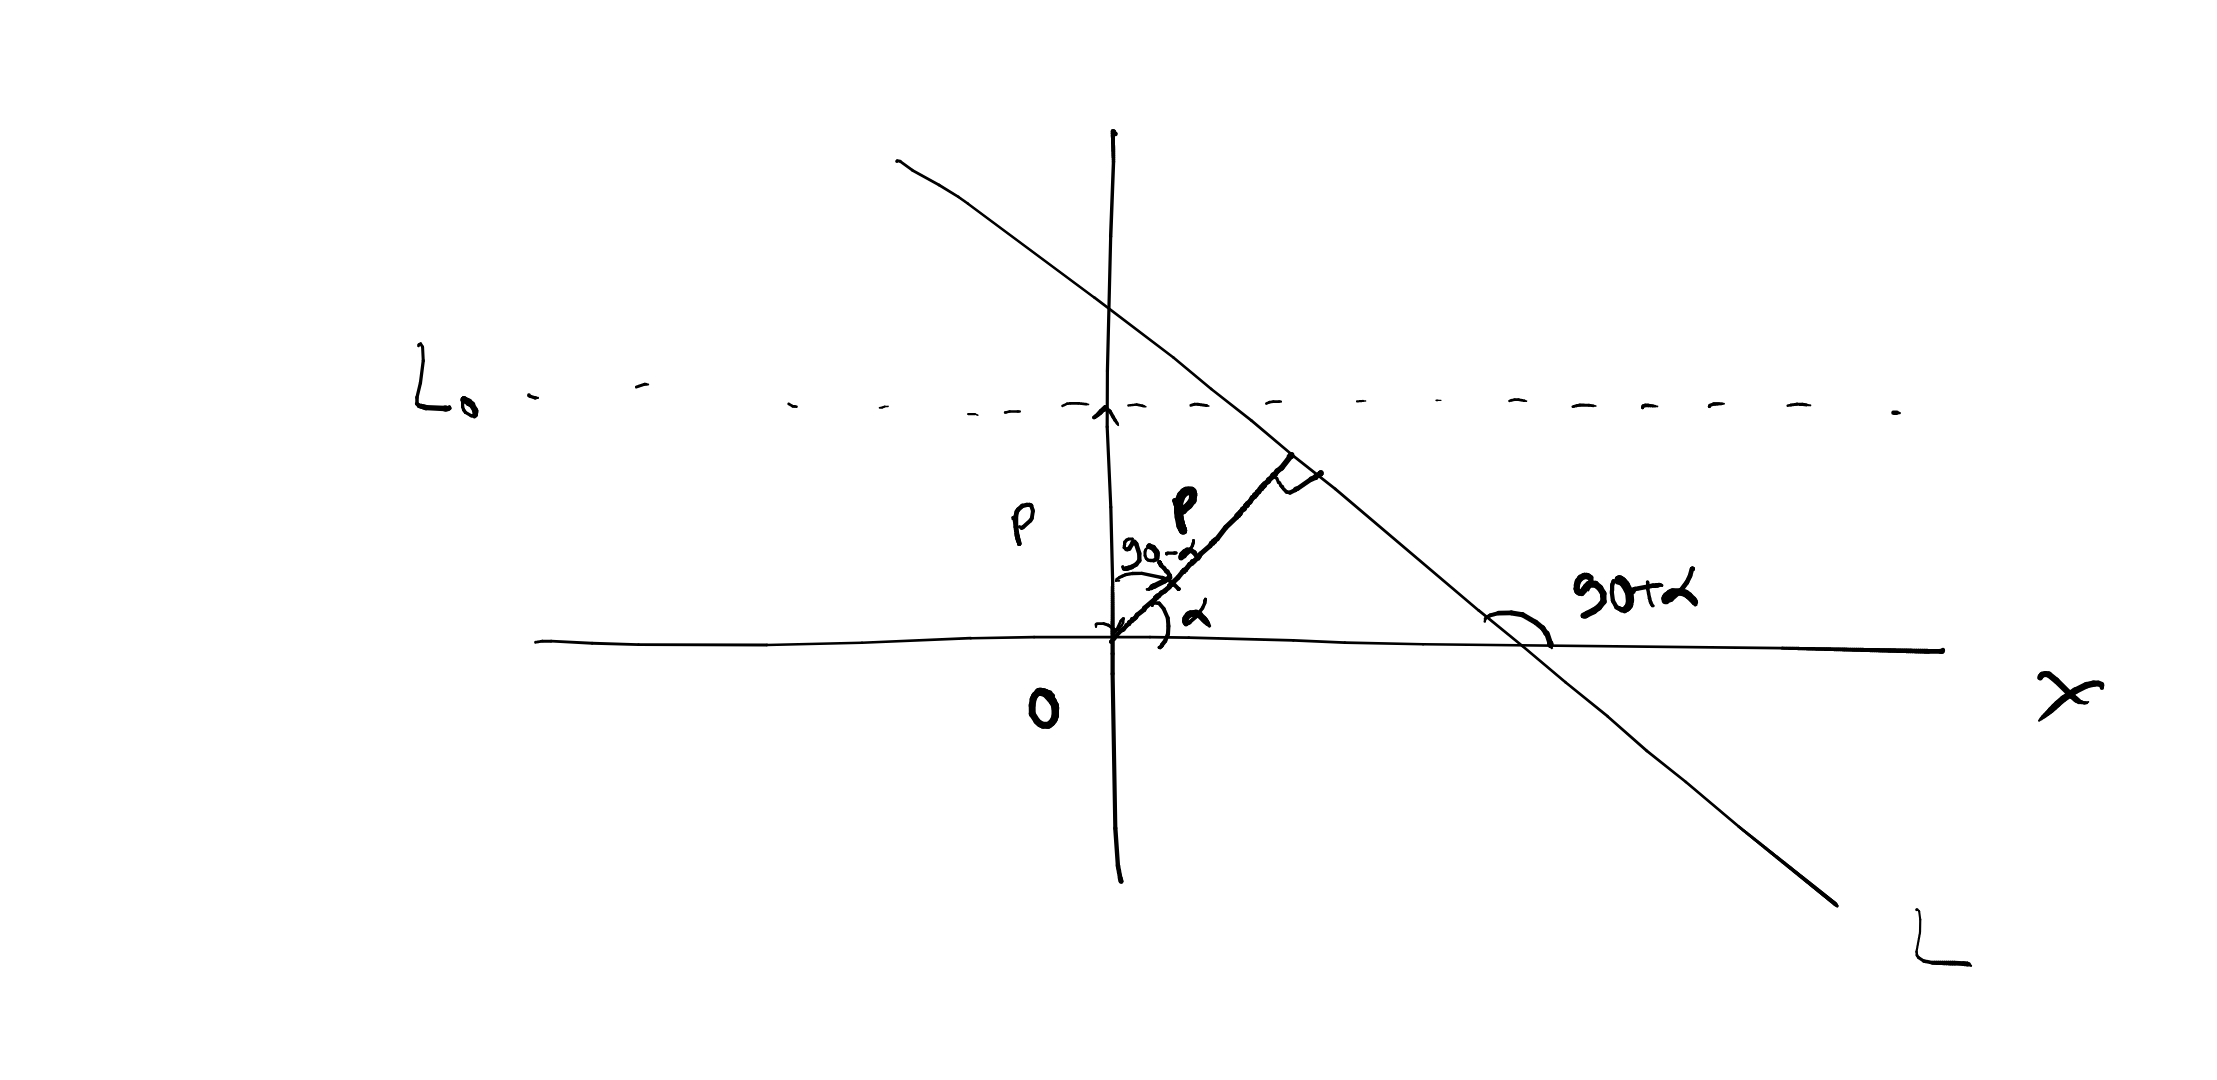
\includegraphics[width=\columnwidth]{./figs/line_dist.eps}
\caption{}
\label{fig:line_dist}
\end{figure}
\item Show that the distance from the orgin to the line 
\begin{align}
\vec{n}^T\vec{x} &=c
\end{align}
is 
\begin{align}
p = \frac{c}{\norm{n}}
\label{eq:line_dist_orig}
\end{align}
\item Show that the point of intersection of two lines 
\begin{align}
\vec{n}_1^T\vec{x} &=c_1
\\
\vec{n}_2^T\vec{x} &=c_2
\end{align}
is given by 
\begin{align}
\vec{x} &=\brak{\vec{N}^T}^{-1}\vec{c}
\end{align}
where 
\begin{align}
\vec{N} = \myvec{\vec{n}_1 & \vec{n}_2}
\end{align}
\item The {\em angle between two lines} is given by 
\begin{align}
\cos ^{-1} \frac{\vec{n}_1 ^T \vec{n}_2}{\norm{\vec{n}_1}  \norm{\vec{n}_2}}
\end{align}
\item Show that the distance of a point $\vec{x}_0$ from the line 
\begin{align}
L: \quad \vec{n}^T\vec{x} &=c
\end{align}
is 
\begin{align}
\frac{\abs{\vec{n}^T\vec{x}_0-c}}{\norm{\vec{n}}} 
\end{align}
\solution Let the equation of the line be 
\begin{align}
\vec{x} = \vec{A} + \lambda \vec{m}
\end{align}
%
where 
\begin{align}
\label{eq:line_dist_orig_pt}
\vec{n}^T\vec{A} = 0, \vec{n}^T\vec{m} = 0
\end{align}
If $\vec{x}_0$ is translated to the origin, the equation of the line $L$ becomes 
\begin{align}
\vec{x} &= \vec{A}- \vec{x}_0+ \lambda \vec{m}
\\
\implies 
\vec{n}^T\vec{x} &=c-\vec{n}^T\vec{x}_0
\end{align}
From \eqref{eq:line_dist_orig}, \eqref{eq:line_dist_orig_pt} is obtained.
\item Show that 
\begin{align}
ax^2+2bxy+cy^2+2dx+2ey+f=0
\end{align}
can be expressed as
\begin{align}
\label{eq:quad_form}
\vec{x}^T\vec{V}\vec{x}+2\vec{u}^T\vec{x}+f=0
\end{align}
%
where
\begin{align}
\vec{V} &= \vec{V}^T
\\
\vec{u} &= \myvec{d & e}
\end{align}

\item {\em Pair of straight lines:} \eqref{eq:quad_form}
%The equation
%\begin{align}
%\vec{x}^T\myvec{a & b\\ b & c}\vec{x}+2\myvec{d & e}+f=0
%\end{align}
%
represents a pair of straight lines if 
\begin{align}
\begin{vmatrix}
\vec{V}&\vec{u}
\\
\vec{u}^T&f
\end{vmatrix}
= 0
\end{align}
%
Two intersecting lines are obtained if 
\begin{align}
\abs{\vec{V}} < 0
\end{align}
\item  In Fig. \ref{fig:ratio}, let
\begin{equation}
\frac{AB}{BC} = \frac{\norm{\vec{A}-\vec{B}}}{\norm{\vec{B}-\vec{C}}} = k.
\label{eq:k}
\end{equation}
%
Show that
\begin{equation}
\frac{\vec{A}+k\vec{C}}{k+1} = \vec{B}.
\label{eq:ratio}
\end{equation}
%
\solution
%
\begin{figure}[!hb]
\centering
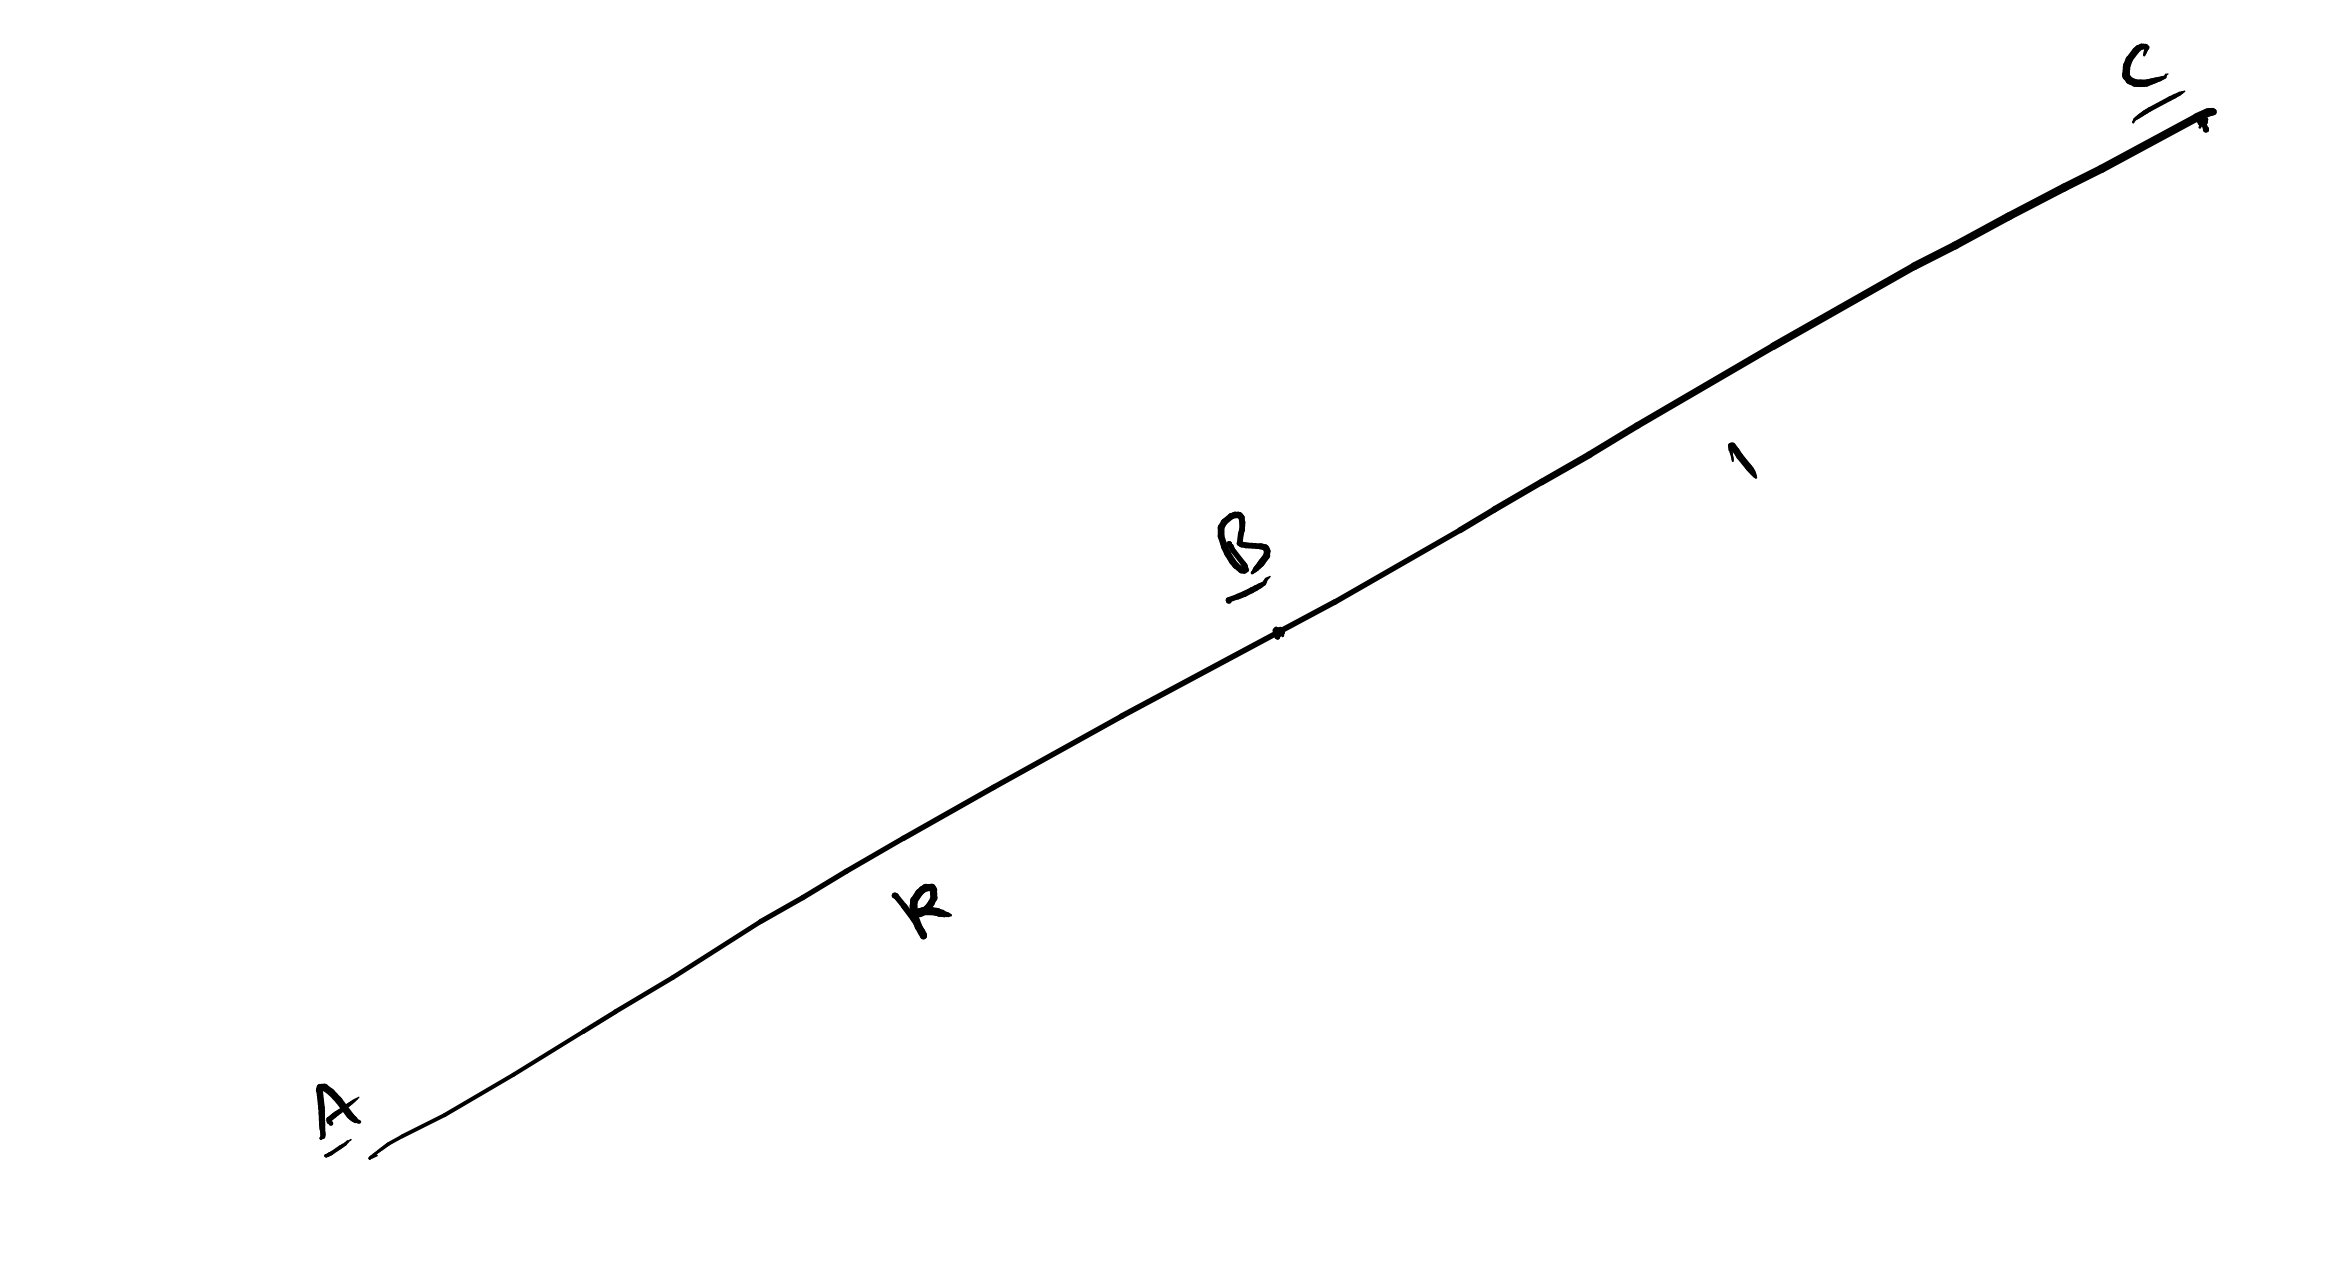
\includegraphics[width=\columnwidth]{./figs/ratio.eps}
\caption{}
\label{fig:ratio}
\end{figure}
From \eqref{eq:nhomog}, 
\begin{align}
\begin{split}
\vec{B} &= \vec{A} + \lambda_1 \vec{m}
\\
\vec{B} &= \vec{C} - \lambda_2 \vec{m}
\end{split}
\\
\label{eq:rat_1}
\implies \frac{\norm{\vec{A}-\vec{B}}}{\norm{\vec{B}-\vec{C}}} &= 
\frac{\lambda_1}{\lambda_2} = k
\\
\text{and } \frac{\vec{B}- \vec{A}}{\lambda_1} &= \frac{\vec{C}- 
\vec{B}}{\lambda_2} = \vec{m},
\label{eq:rat_2}
\end{align}
%
from \eqref{eq:k}. Using \eqref{eq:rat_1} and \eqref{eq:rat_2},
\begin{align}
\vec{A}- \vec{B} &=  k\brak{\vec{B}- \vec{C}}
\end{align}
%
resulting in \eqref{eq:ratio}

%
\item If $\vec{A}$ and $\vec{B}$ are linearly independent,  
\begin{equation}
k_1\vec{A} + k_2\vec{B} = 0 \implies k_1=k_2=0
\end{equation}
\item Show that $\vec{D}$ lies inside $\triangle ABC$ iff
\begin{align}
\vec{D} = \lambda_1\vec{A} + \lambda_2\vec{B} + \lambda_3\vec{C}
\end{align}
such that
\begin{align}
0 \le \lambda_1, \lambda_2, \lambda_3 &\le 1,
\\
0 \le \lambda_1+\lambda_2+\lambda_3 &\le 1,
\end{align}
\item Show that the equation of the angle bisectors of the lines
\begin{align}
\vec{n}_1^T\vec{x} &=c_1
\\
\vec{n}_2^T\vec{x} &=c_2
\end{align}
%
is
\begin{align}
\frac{\vec{n}_1^T\vec{x}-c_1}{\norm{\vec{n}_1}}=\pm\frac{\vec{n}_2^T\vec{x} -c_2}{\norm{\vec{n}_2}}\end{align}
%\item Show that if 
%\begin{align}
%\vec{m}_1 + k\vec{m}_2 \ne 0,
%\end{align}
%%
%there exists $k$ such that for any point $\vec{m}$,
%\begin{align}
%\label{eq:line_basis}
%\vec{m} = \vec{m}_1 + k\vec{m}_2 
%\end{align}
\item Find the equation of a line passing through the intersection of the lines
\begin{align}
\label{eq:line1}
\vec{n}_1^T\vec{x} &=c_1
\\
\vec{n}_2^T\vec{x} &=c_2
\label{eq:line2}
\end{align}
and passing through the point $\vec{p}$.
\\
\solution 
%Let the equation of any line through the intersection of \eqref{eq:line1} and \eqref{eq:line2} be 
%\begin{align}
%\vec{n}^T\vec{x} &=c
%\label{eq:line12}
%\end{align}
%
%If $\vec{u}$ be the point of intersection, 
%\begin{align}
%\myvec{\vec{n}_1^T\\ \vec{n}_2^T\\ \vec{n}^T}\vec{u} &= \myvec{c_1\\c_2\\c}
%\\
%\implies \myvec{\vec{n}_1^T & c_1\\ \vec{n}_2^T & c_2\\ \vec{n}^T & c}&
%\label{eq:line12_mat}
%\end{align}
%has rank 2.  Thus, 
%%
%\begin{align}
%\label{eq:line_basis_normal}
%\myvec{\vec{n}\\c} &= k_1\myvec{\vec{n}_1 \\ c_1}+ k_2\myvec{\vec{n}_2\\c_2} 
%\end{align}
%Substituting in \eqref{eq:line12},
%\begin{align}
%\vec{n}^T\vec{x} = c &
%\implies \vec{n}_1^T\vec{x} + k\vec{n}_2^T\vec{x} =  c_1+kc_2=c
%\label{eq:line_basis_normal_temp}
%\end{align}
%%
%Thus, 
%\begin{align}
%k = \frac{\vec{n}_1^T\vec{p}-c_1}{\vec{n}_2^T\vec{p}-c_2}
%\end{align}
%%
%which can be used to obtain the desired equation using \eqref{eq:line_basis_normal_temp}
%
%Alternatively, 
%
%
The intersection of the lines is 
\begin{align}
\vec{x} = \vec{N}^{-T}\vec{c}
\end{align}
%
where 
\begin{align}
\vec{N} &= \myvec{\vec{n}_1 &\vec{n}_2}
\\
\vec{c} &= \myvec{c_1 \\ c_2} 
\end{align}
Thus, the equation of the desired line is 
\begin{align}
\vec{x} = \vec{p}+ \lambda\brak{\vec{N}^{-T}\vec{c}-\vec{p}}&
\\
\implies \vec{N}^{T}\vec{x} = \vec{N}^{T}\vec{p}+ \lambda\brak{\vec{c}-\vec{N}^{T}\vec{p}}&
\end{align}
resulting in 
\begin{multline}
 \brak{\vec{c}-\vec{N}^T\vec{p}}^T\myvec{0 & -1 \\ 1 & 0}\vec{N}^T\vec{x} 
\\
= \brak{\vec{c}-\vec{N}^T\vec{p}}^T\myvec{0 & -1 \\ 1 & 0}\vec{N}^T\vec{p}
\end{multline}
\item Find $\vec{R}$, the {\em reflection}  of $\vec{P}$ about the line
\begin{align}
L: \quad \vec{n}^T\vec{x} = c
\end{align}
%
\begin{figure}
\centering
\includegraphics[width=\columnwidth]{./figs/reflection.eps}
\caption{}
\label{fig:locus}
\end{figure}
\solution Since $\vec{R}$ is the reflection of $\vec{P}$ and $\vec{Q}$ lies on $L$, $\vec{Q}$ bisects $PR$.  
This leads to the following equations
Hence, 
\begin{align}
\label{eq:reflect_bisect}
2\vec{Q} &= \vec{P}+\vec{R}
\\
\label{eq:reflect_Q}
\vec{n}^{T}\vec{Q} &= c
\\
\label{eq:reflect_R}
\vec{m}^{T}\vec{R} &= \vec{m}^{T}\vec{P}
\end{align}
%
where $\vec{m}$ is the direction vector of $L$.  From \eqref{eq:reflect_bisect} and \eqref{eq:reflect_Q},
\begin{align}
\label{eq:reflect_bisectQ}
\vec{n}^{T}\vec{R}  &= 2c - \vec{n}^{T}\vec{P}
\end{align}
%
From \eqref{eq:reflect_bisectQ} and \eqref{eq:reflect_R},
\begin{align}
\label{eq:reflect_bisectQR}
\myvec{\vec{m} & \vec{n}}^T\vec{R} &= \myvec{\vec{m} & -\vec{n}}^T\vec{P}+ \myvec{0 \\ 2c}
\end{align}
%
Letting 
\begin{align}
\label{eq:reflect_mat}
\vec{V}=  \myvec{\vec{m} & \vec{n}}
\end{align}
with the condition that $\vec{m},\vec{n}$ are orthonormal, i.e.
\begin{align}
\label{eq:reflect_ortho}
\vec{V}^T\vec{V}=  \vec{I}
\end{align}
%
Noting that 
\begin{align}
\label{eq:reflect_trans}
\myvec{\vec{m} & -\vec{n}} &= \myvec{\vec{m} & \vec{n}} \myvec{1 & 0 \\ 0 & -1},
\end{align}
\eqref{eq:reflect_bisectQR} can be expressed as
%
\begin{align}
\label{eq:reflect_}
\vec{V}^T\vec{R} &=  \sbrak{\vec{V}\myvec{1 & 0 \\ 0 & -1}}^T\vec{P}+\myvec{0 \\ 2c}
\\
\implies \vec{R} &= \sbrak{\vec{V}\myvec{1 & 0 \\ 0 & -1}\vec{V}^{-1}}^T\vec{P}+ \vec{V}\myvec{0 \\ 2c}
\\
 &=\vec{V}\myvec{1 & 0 \\ 0 & -1}\vec{V}^T \vec{P}+2c \vec{n}
\end{align}
\item Show that, for any $\vec{m},\vec{n}$, the reflection is also given by
\begin{align}
%\label{eq:reflect_bisect}
\frac{\vec{R}}{2} = \frac{\vec{m}\vec{m}^T-\vec{n}\vec{n}^T}{\vec{m}^T\vec{m}+\vec{n}^T\vec{n}}\vec{P} + c 
\frac{\vec{n}}{\norm{\vec{n}}^2}
\end{align}

\end{enumerate}
%
%
%\item Let $\vec{x}$ be any point on $AB$ in Fi.g \ref{fig:orth}.  Show that
%\begin{equation}
%\brak{\vec{x}-\vec{A}}^T\brak{\vec{B}-\vec{C}} = 0
%\end{equation}
%%
%\item If $\vec{x,y}$ are any two points on $AB$, show that 
%\begin{equation}
%\label{eq:orth_any}
%\brak{\vec{x}-\vec{y}}^T\brak{\vec{B}-\vec{C}} = 0
%\end{equation}
%%
%\item In Fig. \ref{fig:alt}, $BE \perp AC, CF \perp AB$.  Show that $AD \perp BC$.
%\begin{figure}[!hb]
%\centering
%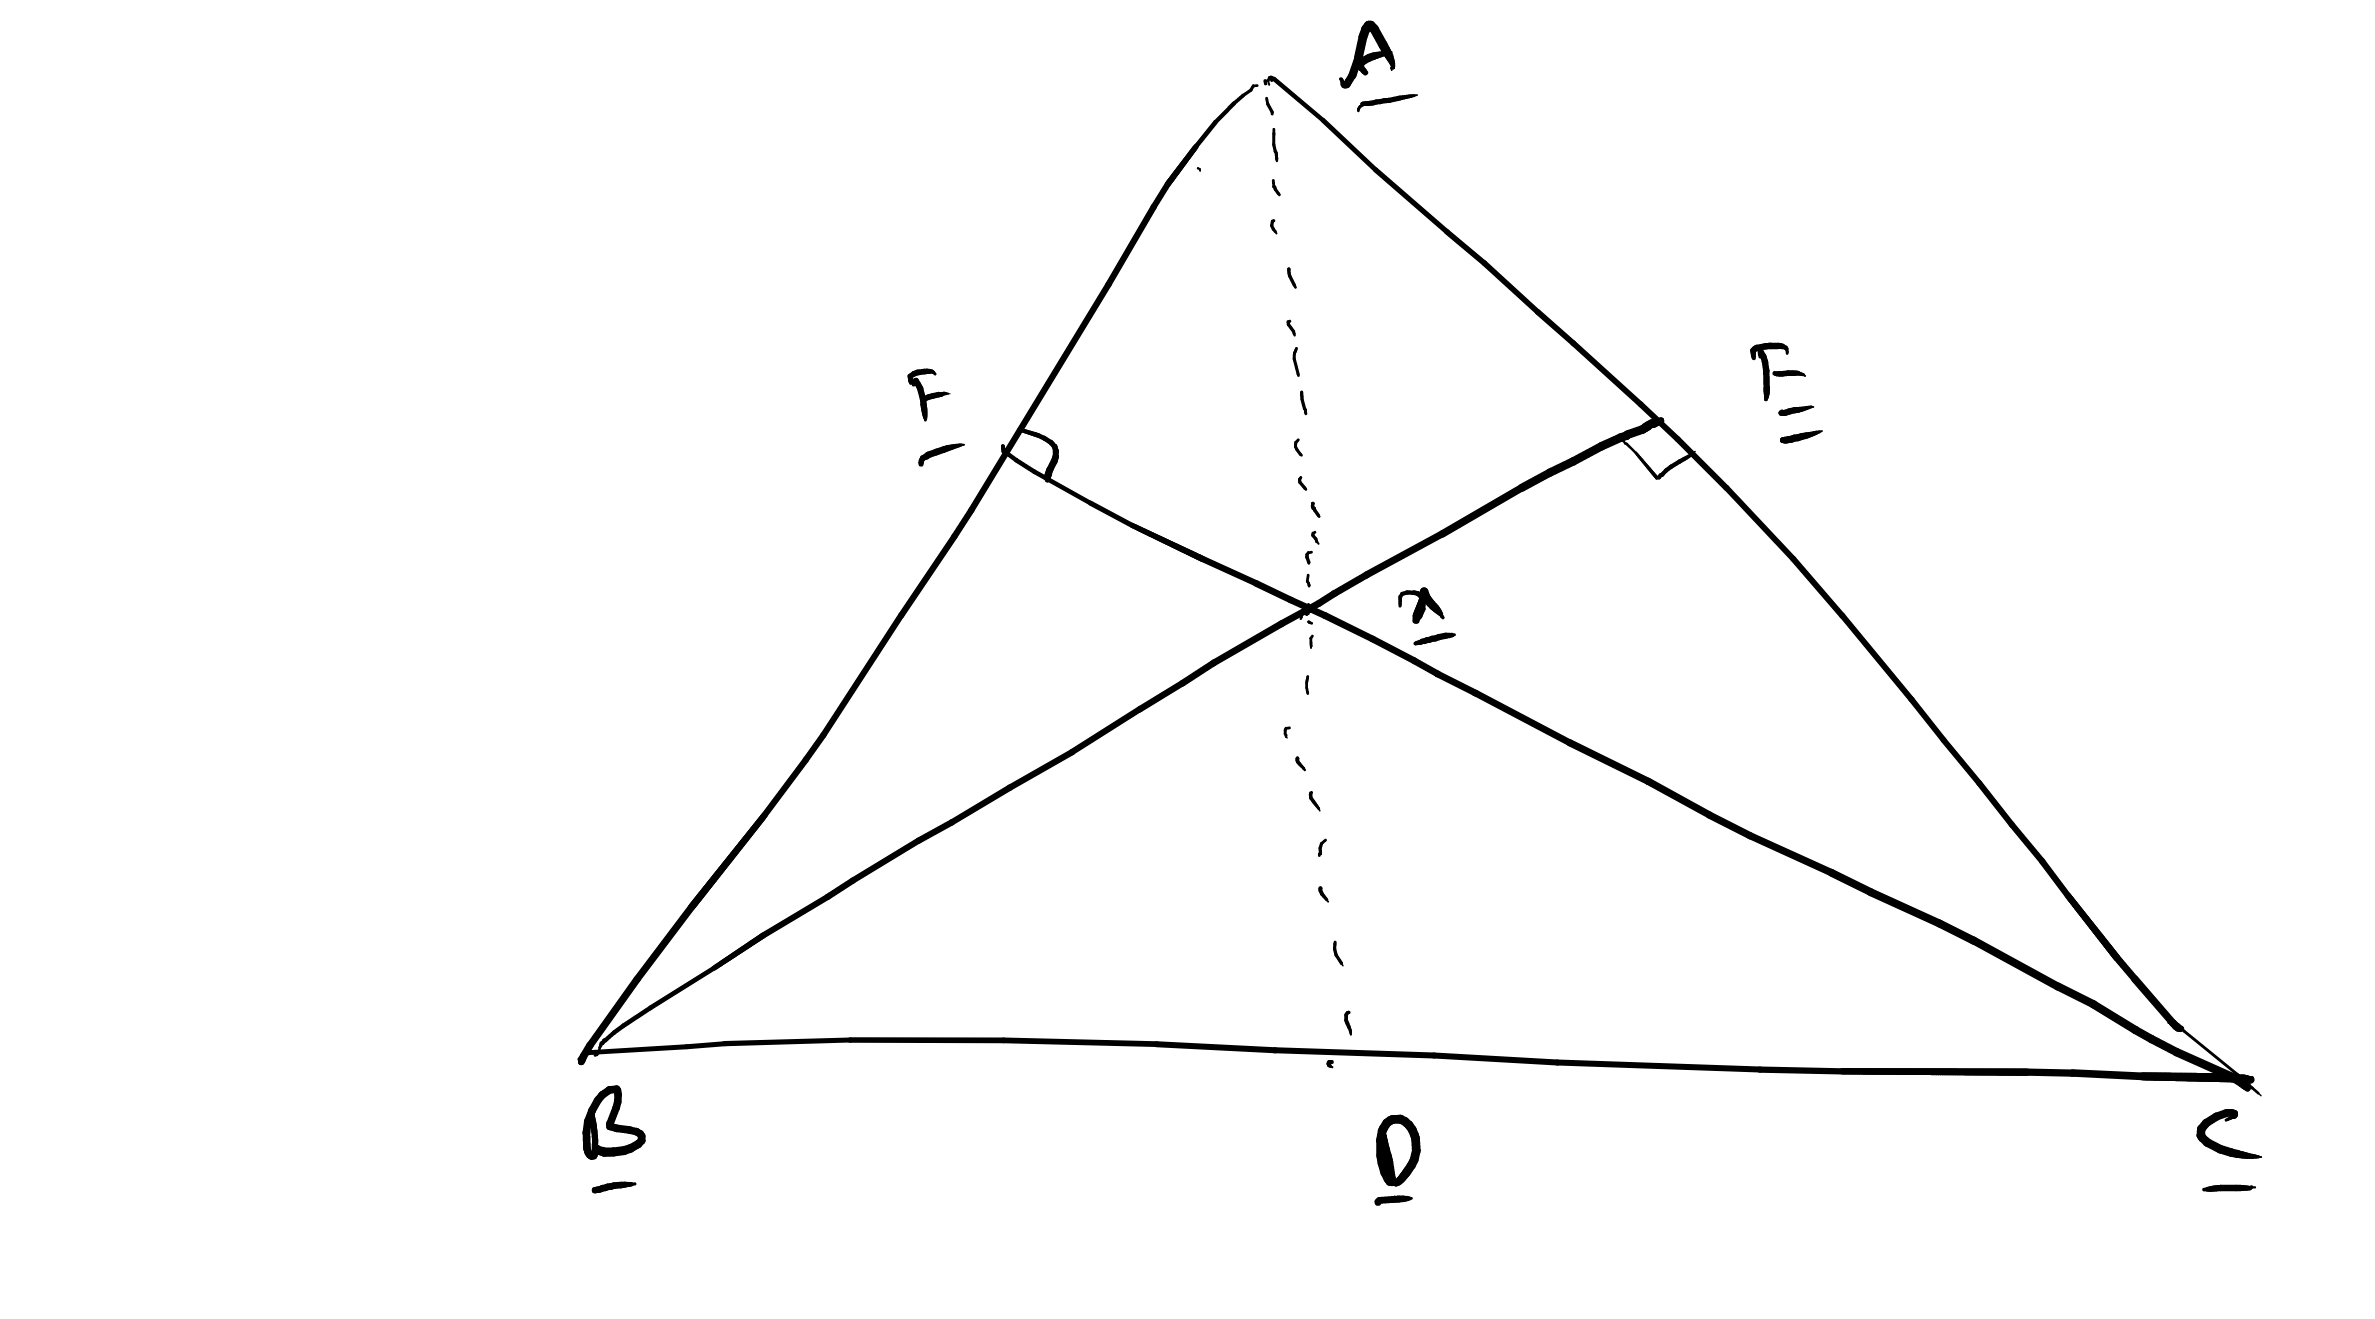
\includegraphics[width=\columnwidth]{./figs/alt.eps}
%\caption{}
%\label{fig:alt}
%\end{figure}
%\\
%\solution Let $\vec{x}$ be the intersection of $BE$ and $CF$. Then, using 
%\eqref{eq:orth_any},
%\begin{align}
%\label{eq:alt_1}
%\begin{split}
%\brak{\vec{x}-\vec{B}}^T
%\brak{\vec{A}-\vec{C}} &= 0
%\\
%\brak{\vec{x}-\vec{C}}^T
%\brak{\vec{A}-\vec{B}} &=0
%\end{split}
%\\
%\label{eq:alt_3}
%\implies \vec{x}^T\brak{\vec{A}-\vec{C}}-\vec{B}^T\brak{\vec{A}-\vec{C}} &= 0
%\\
%\text{and }\vec{x}^T\brak{\vec{A}-\vec{B}}-\vec{C}^T\brak{\vec{A}-\vec{B}} &= 0
%\label{eq:alt_4}
%\end{align}
%%
%Subtracting \eqref{eq:alt_4} from \eqref{eq:alt_3},
%\begin{align}
%\vec{x}^T\brak{\vec{B}-\vec{C}} + \vec{A}^T\brak{\vec{C}-\vec{B}} &= 0
%\\
%\implies \brak{\vec{x}^T - \vec{A}^T}\brak{\vec{B}-\vec{C}}  &= 0
%\\
%\implies \brak{\vec{x} - \vec{A}}^T\brak{\vec{B}-\vec{C}}  &= 0
%\end{align}
%%
%which completes the proof.
%\end{enumerate}
%

\subsection{Programming}
\renewcommand{\theequation}{\theenumi}
\begin{enumerate}[label=\arabic*.,ref=\thesubsection.\theenumi]
\item Find the intercepts made on the axes by the straight lines whose equations are
\begin{multicols}{2}
\begin{enumerate}
%\begin{enumerate}[(i)]
%\setlength\itemsep{2em}
\item
$
\myvec{2 & 3}\vec{x} = 2
$
\item
$
\myvec{1 & -3}\vec{x} = -5
$ 
\item
$
\myvec{1 & -1}\vec{x} = 0
$
\item
$
\myvec{\frac{1}{a+b} & \frac{1}{a-b}}\vec{x} = \frac{1}{a^2-b^2}
$
\item 
$
\myvec{1 & -m}\vec{x} = -c
$
\end{enumerate}
\end{multicols}
\item Write down the equations of straight lines which make the following pairs of intercepts on the axes:
\begin{multicols}{2}
\begin{enumerate}
\item 3,-4
\item -5,6
\item 
$
\frac{1}{a},\frac{1}{b}
$
\item 
$
2a,-2a
$
\end{enumerate}
\end{multicols}
\item A straight line passes through a fixed point $\myvec{h\\k}$ and cuts the axes in $\vec{A},\vec{B}$.  Parallels to the
axes through $\vec{A}$ and $\vec{B}$ intersect in $\vec{P}$.  Find the equation of the locus of $\vec{P}$.
\end{enumerate}

\subsection{Example}
\begin{enumerate}[1.]
\item Find the equations of two straight lines at a distance 3 from the origin and making an angle of $120 \degree$ with $OX$.
\item Find the equation of a straight line making an angle of $60\degree$ with $OX$ and passing through the point $\brak{2,-2}$.
Transform the equation to the form
\begin{equation*}
x\cos\alpha + y\sin \alpha = p 
\end{equation*}
\item Find the equation of the straight line that passes through the points $\brak{2,3}$ and $\brak{3,2}$. What is its inclination
to $OX$?
\item Find the equation of the straight line through the point $\brak{5,7}$ that makes equal intercepts on the axes.
\item Find the equations of the sides of a triangle whose corners are $\brak{2,4}$, $\brak{-4,1}$ and $\brak{2,-3}$.
\item For the same triangle find the equations of the lines joining the corners to the middle points of the opposite sides.
\item Find the equation of a straight line passing through the point $\brak{2,-3}$ parallel to the line $4x-y+7=0$.
\item Find the intercepts on the axes made by a straight line which passes through the point $\brak{3,-1}$ and makes an angle
of $30\degree$ with $OX$.
\item Find the equation of the straight line through the points $\brak{3,-4}$, $\brak{2,3}$ and of the
parallel line through $\brak{5,2}$.
\item What is the distance from the origin of the line $4x-y-7$? Write down the equation of a parallel line at double the distance.
\item Find the equation of the straight line through the point $\brak{3,-4}$ parallel to the line joining the origin to the point
$\brak{2,-1}$.
\item Write down the equation of the straight line which makes intercepts 2 and -7 on the axes, and of the parallel line through
the point $\brak{3,-1}$.
\item Find the equations of the straight line joining the points $\brak{3,4}$, $\brak{-2,1}$ and of the parallel line through
the origin.
\item $ABC$ is a triangle and $A, B$ and $C$ are the points $\brak{2,3}$, $\brak{5,-1}$ and $\brak{-4,2}$.  Find the equation
of the straight line through $A$ parallel to $BC$.
\item Find the equation of a line parallel to $2x+5y=11$ passing through the middle point of the join of the points $\brak{-7,3}$, $\brak{5,-11}$.
\item The base of a triangle passes through a fixed point $\brak{f,g}$ and the sides are bisected at right angles by the axes.  Prove that the locus
of the vertex is the line
\begin{equation*}
gx+fy = 0
\end{equation*}
\end{enumerate}

\subsection{Lagrange Multipliers}
\renewcommand{\theequation}{\theenumi}
\begin{enumerate}[label=\arabic*.,ref=\thesection.\theenumi]
\numberwithin{equation}{enumi}

\item
	\label{convex_code}
Find
\begin{align}
\label{eq:opt_line_nor_h}
	\min_{\mbf{x}}g\brak{\mbf{x}} = \norm{\vec{x}-\vec{P}}^2 = r^2 \\
\text{s.t.} \quad 	h\brak{\mbf{x}} = \vec{n}^T\vec{x} - c = 0\label{eq2_1_line}
%	\quad g\brak{\mbf{x}} = x_1 + x_2 - 9 = 0
\end{align}
by plotting the circles $g\brak{\vec{x}}$
%
%\begin{equation}
% \norm{\vec{x}-\myvec{8\\6}}^2 =r^2
%%(x_1-8)^2 + (x_2-6)^2 = r^2
%\end{equation}
%
% $\mbf{x}= \myvec{x_1\\x_2}$, 
for different values of $r$ along with the line $g\brak{\mbf{x}}$.
%
%\begin{equation}
%\label{eq2_1_line}
%g\brak{\mbf{x}} = \myvec{1 & 1}\vec{x} - 9 = 0
%\end{equation} 
%
\\
\solution 
The following code plots Fig. \ref{fig.concirc}	

%	
\begin{lstlisting}
codes/optimization/concirc.py
\end{lstlisting}

%
\begin{figure}[!ht]
\centering
\includegraphics[width=\columnwidth]{./figs/concirc.eps}
\caption{ Finding $ \displaystyle \min_{\mbf{x}}g\brak{\mbf{x}}$}.
\label{fig.concirc}	
\end{figure}
%
\item By solving the quadratic equation obtained from \eqref{eq:opt_line_nor_h},
show that 
\label{prob:minr}
\begin{align}
\min_{\vec{x}} r = \frac{3}{5}
\end{align}
%
and find $\vec{x} = \vec{Q}$ that minimizes $r$. By labeling  $\vec{Q}$ in Fig. \ref{fig:concirc}, show that $\vec{Q}$ is the point of contact of the line $L$ with the circle of minimum radius $r = \frac{3}{5}$.
%Obtain a theoretical solution for problem \ref{convex_code} 
%%using coordinate geometry.
%
%\solution 
%From \eqref{eq2_1_line} and \eqref{eq2_1_circ}, 
%%
%\begin{align}
%r^2 & = (x_1-8)^2 + (3- x_1)^2 \\
%&= 2 x_1^2 - 22 x_1 + 73 \\
%\Rightarrow r^2 &= \frac{\brak{2x_1-11}^2 + 5^2}{2}
%\end{align}
%%
%which is minium when $x_1 = \frac{11}{2}, x_2 = \frac{7}{2}$.  The minimum value is $\frac{25}{2}$ and 
%the radius $r = \frac{5}{\sqrt{2}}$.
\item Show that 
\begin{align}
\nabla h(\vec{x}) =  \myvec{3 \\ -4} = \vec{n}
\end{align}
where
\begin{equation}
\nabla =  
\begin{pmatrix}
\frac{\partial}{\partial x_1} \\
\frac{\partial}{\partial x_2} 
\end{pmatrix}
\end{equation}

\item Show that 
\begin{align}
\nabla g(\vec{x}) = 2\cbrak{\vec{x}-\myvec{3 \\ -5}} = 2\cbrak{\vec{x}-\vec{P}}
\end{align}
%
%is the direction vector of the normal at $\vec{x}$.
\item From Fig. \ref{fig.concirc}, show that 
\begin{align}
\label{eq:opt_normal}
\nabla g(\vec{Q}) = \lambda \nabla h(\vec{Q}),
\end{align}
%
%where $\vec{p}$ is the point of contact.
\item Use \eqref{eq:opt_normal} and $\vec{h(\vec{Q})}=0$ from \eqref{eq2_1_line} to obtain $\vec{Q}$.
\item
\label{lagrange}
	Define 
	\begin{equation}
	\label{lagrangian}
	C\brak{\mbf{x},\lambda} = g\brak{\mbf{x}} - \lambda h\brak{\mbf{x}}%, \quad \lambda > 0
	\end{equation}
and show that $\vec{Q}$ can also be obtained by 
solving the equations
%
\begin{align}
\nabla C\brak{\mbf{x},\lambda} &= 0.
\label{tangent}
\end{align}
%
What is the sign of $\lambda$?  $C$ is known as the Lagrangian and the above technique is known as the Method of Lagrange Multipliers.

\solution
%From \eqref{eq2_1_line} and \eqref{eq2_1_circ}, 
%%
%\begin{align}
%L\brak{\mbf{x},\lambda} &= (x_1-8)^2 + (x_2-6)^2 - \lambda \brak{x_1 + x_2 - 9} \\
%\Rightarrow \nabla L\brak{\mbf{x},\lambda}  & = 
%\begin{pmatrix}
%2x_1  - 16 - \lambda \\
%2x_2 - 12 - \lambda \\
%x_1 + x_2 -9
%\end{pmatrix}
%\\
%&=
%\begin{pmatrix}
%2 &0 & - 1 \\
%0 &2 & - 1 \\
%1 & 1 & 0 
%\end{pmatrix}
%\begin{pmatrix}
%x_1 \\
%x_2 \\
%\lambda
%\end{pmatrix}
%= 
%\begin{pmatrix}
%16 \\
% 12 \\
%9
%\end{pmatrix}
%=
%0 
%\\
%\Rightarrow 
%\begin{pmatrix}
%x_1 \\
%x_2 \\
%\lambda
%\end{pmatrix}
%&= 
%\begin{pmatrix}
%\frac{11}{2} \\
% \frac{7}{2} \\
%-5
%\end{pmatrix}
%\end{align}
%%
%using the following python script.  Note that this method yields the same result as the previous exercises.  Thus, $\lambda$ is negative.
%	
\begin{lstlisting}
codes/optimization/lagmul.py
\end{lstlisting}
\item Obtain $\vec{Q}$ using gradient descent.
\end{enumerate}

\subsection{Inequality Constraints}
\renewcommand{\theequation}{\theenumi}
\begin{enumerate}[label=\arabic*.,ref=\thesubsection.\theenumi]
\numberwithin{equation}{enumi}

%
\item
\label{ch2_constraint}
Modify the code in problem \ref{convex_code} to find a graphical solution for minimising
\begin{align}
f\brak{\mbf{x}} 
%= (x_1-8)^2 + (x_2-6)^2
\end{align}
with constraint
\begin{align}
%\label{convex-constraint}
g\brak{\mbf{x}} \geq 0
%= x_1 + x_2 - 9 
\end{align}

\solution 
This problem reduces to finding the radius of the smallest circle in the shaded area in Fig. \ref{fig.2.4} .  It is clear that this radius is 0.
%	
\begin{lstlisting}
codes/optimization/2.4.py
\end{lstlisting}

%
\begin{figure}[!ht]
\centering
\includegraphics[width=\columnwidth]{./optimization/figs/2.4.eps}
\caption{ Smallest circle in the shaded region is a point.}
\label{fig.2.4}	
\end{figure}
%
\item
\label{ch2_lagrange_fail}
Now use the method of Lagrange multipliers to solve  problem \ref{ch2_constraint} and compare with the graphical solution.  Comment.

%
\solution Using the method of Lagrange multipliers, the solution is the same as the one obtained in  problem \ref{ch2_constraint}, which is different from the graphical solution.  This means that the Lagrange multipliers method cannot be applied blindly.
\item
Repeat problem \ref{ch2_lagrange_fail} by keeping 
 $\lambda=0$.   Comment.

\solution Keeping $\lambda = 0$ results in $\vec{x}=\myvec{ 8\\ 6}$, which is the correct solution.  The minimum value of $f\brak{\mbf{x}}$ without any constraints lies in the region $g\brak{\mbf{x}} = 0$.  In this case, $\lambda = 0$.  
%
%
\item
\label{ch2_constraint_border}
Find a graphical solution for minimising
\begin{align}
f\brak{\mbf{x}}
% = (x_1-8)^2 + (x_2-6)^2
\end{align}
with constraint
\begin{align}
%\label{convex-constraint}
g\brak{\mbf{x}} \leq 0
%= x_1 + x_2 - 9 .
\end{align}
Summarize your observations.

%
\solution In Fig. \ref{fig.2.7}, the shaded region represents the constraint.  Thus, the solution is the same as the one in problem \ref{ch2_constraint}. This implies that the method of
Lagrange multipliers can be used to solve the optimization problem with this inequality constraint as well.  Table \ref{table.2.7} summarizes the conditions for this based on the observations so far.
\begin{lstlisting}
codes/optimization/2.7.py
\end{lstlisting}

%
\begin{figure}[!ht]
\centering
\includegraphics[width=\columnwidth]{./optimization/figs/2.7.eps}
\caption{ Finding $ \displaystyle \min_{\mbf{x}}f\brak{\mbf{x}}$.}
\label{fig.2.7}	
\end{figure}
%%%%%%%%%%%%%%%%%%%%%%%%%%%%%%%%%%%%%%%%%%%%%%%%%%%%%%%%%%%%%%%%%%%%%%
%%                                                                  %%
%%  This is the header of a LaTeX2e file exported from Gnumeric.    %%
%%                                                                  %%
%%  This file can be compiled as it stands or included in another   %%
%%  LaTeX document. The table is based on the longtable package so  %%
%%  the longtable options (headers, footers...) can be set in the   %%
%%  preamble section below (see PRAMBLE).                           %%
%%                                                                  %%
%%  To include the file in another, the following two lines must be %%
%%  in the including file:                                          %%
%%        \def\inputGnumericTable{}                                 %%
%%  at the beginning of the file and:                               %%
%%        \input{name-of-this-file.tex}                             %%
%%  where the table is to be placed. Note also that the including   %%
%%  file must use the following packages for the table to be        %%
%%  rendered correctly:                                             %%
%%    \usepackage[latin1]{inputenc}                                 %%
%%    \usepackage{color}                                            %%
%%    \usepackage{array}                                            %%
%%    \usepackage{longtable}                                        %%
%%    \usepackage{calc}                                             %%
%%    \usepackage{multirow}                                         %%
%%    \usepackage{hhline}                                           %%
%%    \usepackage{ifthen}                                           %%
%%  optionally (for landscape tables embedded in another document): %%
%%    \usepackage{lscape}                                           %%
%%                                                                  %%
%%%%%%%%%%%%%%%%%%%%%%%%%%%%%%%%%%%%%%%%%%%%%%%%%%%%%%%%%%%%%%%%%%%%%%



%%  This section checks if we are begin input into another file or  %%
%%  the file will be compiled alone. First use a macro taken from   %%
%%  the TeXbook ex 7.7 (suggestion of Han-Wen Nienhuys).            %%
\def\ifundefined#1{\expandafter\ifx\csname#1\endcsname\relax}


%%  Check for the \def token for inputed files. If it is not        %%
%%  defined, the file will be processed as a standalone and the     %%
%%  preamble will be used.                                          %%
\ifundefined{inputGnumericTable}

%%  We must be able to close or not the document at the end.        %%
	\def\gnumericTableEnd{\end{document}}


%%%%%%%%%%%%%%%%%%%%%%%%%%%%%%%%%%%%%%%%%%%%%%%%%%%%%%%%%%%%%%%%%%%%%%
%%                                                                  %%
%%  This is the PREAMBLE. Change these values to get the right      %%
%%  paper size and other niceties.                                  %%
%%                                                                  %%
%%%%%%%%%%%%%%%%%%%%%%%%%%%%%%%%%%%%%%%%%%%%%%%%%%%%%%%%%%%%%%%%%%%%%%

	\documentclass[12pt%
			  %,landscape%
                    ]{report}
       \usepackage[latin1]{inputenc}
       \usepackage{fullpage}
       \usepackage{color}
       \usepackage{array}
       \usepackage{longtable}
       \usepackage{calc}
       \usepackage{multirow}
       \usepackage{hhline}
       \usepackage{ifthen}

	\begin{document}


%%  End of the preamble for the standalone. The next section is for %%
%%  documents which are included into other LaTeX2e files.          %%
\else

%%  We are not a stand alone document. For a regular table, we will %%
%%  have no preamble and only define the closing to mean nothing.   %%
    \def\gnumericTableEnd{}

%%  If we want landscape mode in an embedded document, comment out  %%
%%  the line above and uncomment the two below. The table will      %%
%%  begin on a new page and run in landscape mode.                  %%
%       \def\gnumericTableEnd{\end{landscape}}
%       \begin{landscape}


%%  End of the else clause for this file being \input.              %%
\fi

%%%%%%%%%%%%%%%%%%%%%%%%%%%%%%%%%%%%%%%%%%%%%%%%%%%%%%%%%%%%%%%%%%%%%%
%%                                                                  %%
%%  The rest is the gnumeric table, except for the closing          %%
%%  statement. Changes below will alter the table's appearance.     %%
%%                                                                  %%
%%%%%%%%%%%%%%%%%%%%%%%%%%%%%%%%%%%%%%%%%%%%%%%%%%%%%%%%%%%%%%%%%%%%%%

\providecommand{\gnumericmathit}[1]{#1} 
%%  Uncomment the next line if you would like your numbers to be in %%
%%  italics if they are italizised in the gnumeric table.           %%
%\renewcommand{\gnumericmathit}[1]{\mathit{#1}}
\providecommand{\gnumericPB}[1]%
{\let\gnumericTemp=\\#1\let\\=\gnumericTemp\hspace{0pt}}
 \ifundefined{gnumericTableWidthDefined}
        \newlength{\gnumericTableWidth}
        \newlength{\gnumericTableWidthComplete}
        \newlength{\gnumericMultiRowLength}
        \global\def\gnumericTableWidthDefined{}
 \fi
%% The following setting protects this code from babel shorthands.  %%
 \ifthenelse{\isundefined{\languageshorthands}}{}{\languageshorthands{english}}
%%  The default table format retains the relative column widths of  %%
%%  gnumeric. They can easily be changed to c, r or l. In that case %%
%%  you may want to comment out the next line and uncomment the one %%
%%  thereafter                                                      %%
\providecommand\gnumbox{\makebox[0pt]}
%%\providecommand\gnumbox[1][]{\makebox}

%% to adjust positions in multirow situations                       %%
\setlength{\bigstrutjot}{\jot}
\setlength{\extrarowheight}{\doublerulesep}

%%  The \setlongtables command keeps column widths the same across  %%
%%  pages. Simply comment out next line for varying column widths.  %%
\setlongtables

\setlength\gnumericTableWidth{%
	53pt+%
	58pt+%
	55pt+%
0pt}
\def\gumericNumCols{3}
\setlength\gnumericTableWidthComplete{\gnumericTableWidth+%
         \tabcolsep*\gumericNumCols*2+\arrayrulewidth*\gumericNumCols}
\ifthenelse{\lengthtest{\gnumericTableWidthComplete > \linewidth}}%
         {\def\gnumericScale{\ratio{\linewidth-%
                        \tabcolsep*\gumericNumCols*2-%
                        \arrayrulewidth*\gumericNumCols}%
{\gnumericTableWidth}}}%
{\def\gnumericScale{1}}

%%%%%%%%%%%%%%%%%%%%%%%%%%%%%%%%%%%%%%%%%%%%%%%%%%%%%%%%%%%%%%%%%%%%%%
%%                                                                  %%
%% The following are the widths of the various columns. We are      %%
%% defining them here because then they are easier to change.       %%
%% Depending on the cell formats we may use them more than once.    %%
%%                                                                  %%
%%%%%%%%%%%%%%%%%%%%%%%%%%%%%%%%%%%%%%%%%%%%%%%%%%%%%%%%%%%%%%%%%%%%%%

\ifthenelse{\isundefined{\gnumericColA}}{\newlength{\gnumericColA}}{}\settowidth{\gnumericColA}{\begin{tabular}{@{}p{53pt*\gnumericScale}@{}}x\end{tabular}}
\ifthenelse{\isundefined{\gnumericColB}}{\newlength{\gnumericColB}}{}\settowidth{\gnumericColB}{\begin{tabular}{@{}p{58pt*\gnumericScale}@{}}x\end{tabular}}
\ifthenelse{\isundefined{\gnumericColC}}{\newlength{\gnumericColC}}{}\settowidth{\gnumericColC}{\begin{tabular}{@{}p{55pt*\gnumericScale}@{}}x\end{tabular}}

\begin{table}[!h]
	\caption{Summary of conditions.} 
	\centering
\begin{tabular}[c]{%
	b{\gnumericColA}%
	b{\gnumericColB}%
	b{\gnumericColC}%
	}

%%%%%%%%%%%%%%%%%%%%%%%%%%%%%%%%%%%%%%%%%%%%%%%%%%%%%%%%%%%%%%%%%%%%%%
%%  The longtable options. (Caption, headers... see Goosens, p.124) %%            \\	%
 %\hline	% Across the top of the table.
%%  The rest of these options are table rows which are placed on    %%
%%  the first, last or every page. Use \multicolumn if you want.    %%

%%  Header for the first page.                                      %%
%	\multicolumn{3}{c}{The First Header} \\ \hline 
%	\multicolumn{1}{c}{colTag}	%Column 1
%	&\multicolumn{1}{c}{colTag}	%Column 2
%	&\multicolumn{1}{c}{colTag}	\\ \hline %Last column
%	\endfirsthead

%%  The running header definition.                                  %%
%	\hline
%	\multicolumn{3}{l}{\ldots\small\slshape continued} \\ \hline
%	\multicolumn{1}{c}{colTag}	%Column 1
%	&\multicolumn{1}{c}{colTag}	%Column 2
%	&\multicolumn{1}{c}{colTag}	\\ \hline %Last column
%	\endhead

%%  The running footer definition.                                  %%
%	\hline
%	\multicolumn{3}{r}{\small\slshape continued\ldots} \\
%	\endfoot

%%  The ending footer definition.                                   %%
%	\multicolumn{3}{c}{That's all folks} \\ \hline 
%	\endlastfoot
%%%%%%%%%%%%%%%%%%%%%%%%%%%%%%%%%%%%%%%%%%%%%%%%%%%%%%%%%%%%%%%%%%%%%%

\hhline{|-|-|-}
	 \multicolumn{1}{|p{\gnumericColA}|}%
	{\gnumericPB{\centering}\textbf{Cost}}
	&\multicolumn{1}{p{\gnumericColB}|}%
	{\gnumericPB{\centering}\textbf{Constraint}}
	&\multicolumn{1}{p{\gnumericColC}|}%
	{\gnumericPB{\centering}\textbf{$\lambda$}}
\\
\hhline{|---|}
	 \multicolumn{1}{|p{\gnumericColA}|}%
	{\setlength{\gnumericMultiRowLength}{0pt}%
	 \addtolength{\gnumericMultiRowLength}{\gnumericColA}%
	 \multirow{3}[1]{\gnumericMultiRowLength}{\parbox{\gnumericMultiRowLength}{%
	 \gnumericPB{\centering}$f\brak{\mbf{x}}$}}}
	&\multicolumn{1}{p{\gnumericColB}|}%
	{\gnumericPB{\centering}$g\brak{\mbf{x}} = 0$}
	&\multicolumn{1}{p{\gnumericColC}|}%
	{\gnumericPB{\centering} $<$ 0}
\\
\hhline{~|--|}
	 \multicolumn{1}{|p{\gnumericColA}|}%
	{}
	&\multicolumn{1}{p{\gnumericColB}|}%
	{\gnumericPB{\centering}$g\brak{\mbf{x}} \geq 0 $}
	&\multicolumn{1}{p{\gnumericColC}|}%
	{\gnumericPB{\centering}0}
\\
\hhline{~|--|}
	 \multicolumn{1}{|p{\gnumericColA}|}%
	{}
	&\multicolumn{1}{p{\gnumericColB}|}%
	{\gnumericPB{\centering}$g\brak{\mbf{x}}\leq 0 $}
	&\multicolumn{1}{p{\gnumericColC}|}%
	{\gnumericPB{\centering} $<$ 0}
\\
\hhline{|-|-|-|}
\end{tabular}
\label{table.2.7}
\end{table}

\ifthenelse{\isundefined{\languageshorthands}}{}{\languageshorthands{\languagename}}
\gnumericTableEnd

%
\item
\label{ch2_prob_upper}
Find a graphical solution for 	 
	 \begin{align}
	 \label{ch2_second_min}
	\min_{\mbf{x}} f\brak{\mbf{x}} = \norm{\vec{x}-\myvec{8\\6}}^2
	 \end{align}
	 with constraint
	 \begin{align}
	 \label{ch2_second_const}
	 g\brak{\mbf{x}} = \myvec{1 & 1}\vec{x} - 18 = 0
	 \end{align}
	 
%
\solution
%	
\begin{lstlisting}
codes/optimization/2.8.py
\end{lstlisting}

%
\begin{figure}[!ht]
\centering
\includegraphics[width=\columnwidth]{./optimization/figs/2.8.eps}
\caption{ Finding $ \displaystyle \min_{\mbf{x}}f\brak{\mbf{x}}$.}
\label{fig.2.8}	
\end{figure}
%
\item
Repeat problem \ref{ch2_prob_upper} using the method of Lagrange mutipliers.  What is the sign of $\lambda$?

%
\solution
%From \eqref{ch2_second_min} and \eqref{ch2_second_const}, 
%%
%\begin{align}
%L\brak{\mbf{x},\lambda} &= (x_1-8)^2 + (x_2-6)^2 - \lambda \brak{x_1 + x_2 - 18} \\
%\Rightarrow \nabla L\brak{\mbf{x},\lambda}  & = 
%\begin{pmatrix}
%2x_1  - 16 - \lambda \\
%2x_2 - 12 - \lambda \\
%x_1 + x_2 -18
%\end{pmatrix}
%\\
%&=
%\begin{pmatrix}
%2 &0 & - 1 \\
%0 &2 & - 1 \\
%1 & 1 & 0 
%\end{pmatrix}
%\begin{pmatrix}
%x_1 \\
%x_2 \\
%\lambda
%\end{pmatrix}
%= 
%\begin{pmatrix}
%16 \\
% 12 \\
%18
%\end{pmatrix}
%=
%0 
%\\
%\Rightarrow 
%\begin{pmatrix}
%x_1 \\
%x_2 \\
%\lambda
%\end{pmatrix}
%&= 
%\begin{pmatrix}
%10 \\
% 8 \\
%4
%\end{pmatrix}
%\end{align}
%%
Using the following python script, $\lambda$ is positive and the minimum value of $f$ is 8.
%	
\begin{lstlisting}
codes/optimization/2.9.py
\end{lstlisting}

%
%
\item
\label{ch2_prob_upper_cond}
Solve
	 \begin{align}
%	 \label{ch2_second_min}
	\min_{\mbf{x}} f\brak{\mbf{x}} 
%= (x_1-8)^2 + (x_2-6)^2
	 \end{align}
	 with constraint
	 \begin{align}
%	 \label{ch2_second_const}
	 g\brak{\mbf{x}} 
%= x_1 + x_2 - 18 
\geq 0 
	 \end{align}
	 
%
\solution Since the unconstrained solution is outside the region $g\brak{\mbf{x}} \geq 0$, the solution is the same as the one in problem \ref{ch2_prob_upper}.
%
\item
Based on the problems so far, generalise the Lagrange multipliers method for 
%
	 \begin{align}
	 \label{ch2_lagrange_ineq}
	\min_{\mbf{x}} f\brak{\mbf{x}} , \quad 
	 g\brak{\mbf{x}}  \geq 0 
	 \end{align}
%

%
\solution
Considering $L\brak{\mbf{x},\lambda} = f\brak{\mbf{x}} - \lambda g\brak{\mbf{x}}$, for $g\brak{\mbf{x}} = \myvec{1 & 1}\vec{x} - 18 \geq 0$ we found $\lambda > 0 $ and for $g\brak{\mbf{x}} = \myvec{1 & 1}\vec{x} - 9 \leq 0, \lambda < 0$. A single condition can be obtained by framing the optimization problem as
%
	 \begin{align}
	 \label{ch2_lagrange_ineq_summary}
	\min_{\mbf{x}} f\brak{\mbf{x}} , \quad 
	 g\brak{\mbf{x}}  \leq 0 
	 \end{align}
%
with the Lagrangian
%
\begin{equation}
%\label{ch2_kkt_necessary}
L\brak{\mbf{x},\lambda} = f\brak{\mbf{x}} + \lambda g\brak{\mbf{x}}, %\quad  \lambda > 0,  g\brak{\mbf{x}} \leq 0.
\end{equation}
%
provided
%
\begin{equation}
\label{ch2_kkt_necessary}
\nabla L\brak{\mbf{x},\lambda} = 0 \Rightarrow \lambda > 0
\end{equation}
else, $\lambda = 0$.

%
\item
	\label{convex_sdp_eqiv}
	%
	Solve
	\begin{equation}
	\min_{\mbf{x}} \quad x_1 + x_2
	\end{equation}
	%	
	with the constraints
	\begin{equation}
	x_1^2 - x_1 + x_2^2 \leq 0
	\end{equation}
	%
where 
$
\mbf{x} = \begin{pmatrix}
x_1 \\
x_2
\end{pmatrix}
$

\solution 
%Using the method of Lagrange multipliers,
%%
%\begin{align}
%\label{ch2_sd_kkt}
%\nabla \cbrak{f(\mbf{x})  +  \mu g(\mbf{x}) }= 0 , \quad \mu \ge 0
%\end{align}
%%
%resulting in the equations
%%
%\begin{align}
%2x_1\mu -\mu + 1 &= 0 \\
%2x_2\mu + 1 &=0 \\
%x_1^2 -x_1 + x_2^2 &= 0 
%\end{align}
%%
%which can be simplified to obtain 
%%
%\begin{align}
%\brak{\frac{1-\mu}{2\mu}}^2 + \brak{\frac{1}{2\mu}}^2 + \frac{1-\mu}{2\mu} &= 0 \\
%\Rightarrow 1 + \mu^2 -2\mu + 1 + 2\mu\brak{1-\mu} &= 0 \\
%\Rightarrow \mu^2 =2, or \mu &= \pm \sqrt{2} 
%\end{align}
%%
%From \eqref{ch2_kkt_problem},  $\mu \ge 0 \Rightarrow  \mu = \sqrt{2}$. The desired solution is
%%
%\begin{equation}
%\mbf{x} = 
%\begin{pmatrix}
% \frac{\sqrt{2}-1}{2\sqrt{2}} \\
%-\frac{1}{2\sqrt{2}} 
%\end{pmatrix}
%\end{equation}
%
\\
{\em Graphical solution:} 
%The constraint can be expressed as
%%
%\begin{align}
%x_1^2 - x_1 + x_2^2 &\le 0 \\
%\Rightarrow \brak{x_1 - \frac{1}{2}}^2 + x_2^2 & \le \brak{\frac{1}{2}}^2
%\end{align}
%
%	
\begin{lstlisting}
codes/optimization/2.15.py
\end{lstlisting}

%
%
\begin{figure}[!ht]
\centering
\includegraphics[width=\columnwidth]{./optimization/figs/2.15.eps}
\caption{ Optimal solution is the lower tangent to the circle}
\label{fig.2.15}	
\end{figure}
\end{enumerate}

\subsection{Solved Problems}
\renewcommand{\theequation}{\theenumi}
\begin{enumerate}[label=\arabic*.,ref=\thesubsection.\theenumi]
\item Find the distance of the point $\myvec{4\\2\sqrt{3}}$ from the line 
\begin{equation}
\myvec{\cos 60\degree &  \sin 60\degree}\vec{x} = 6
\end{equation}
\numberwithin{equation}{enumi}
\item Find the distance of the point $\myvec{2\\3}$ from each of the straight lines 
\begin{align}
\myvec{5&12}\vec{x}-20&=0
\\
 \myvec{4&-3}\vec{x}+11&=0
\\
 \myvec{3 & 4}\vec{x}-28&=0.
\end{align}
\renewcommand{\theequation}{\theenumi}
\item Find the distance of the pont $\myvec{3\\-1}$ from the line joining the points $\myvec{2\\-3}$, $\myvec{4\\1}$.
\item Are the points $\myvec{-2\\3}$, $\myvec{-2\\4}$ on the same or on opposite sides of the line
\begin{align}
\myvec{4 &5} \vec{x}= 10?
\end{align}
\numberwithin{equation}{enumi}
\item Find the equations of the bisectors of the angles between the lines
\begin{align}
\myvec{-4 &2}\vec{x}&=-9
\\
\myvec{-1 & 2}\vec{x}&= 4
\end{align}
and state which equation refers to the angle which contains the origin.
\item Prove that the bisector of one of the angles between the lines
\begin{align}
\myvec{5&1}\vec{x}-7 &= 0
\\
\myvec{1 & -5}\vec{x}+7 &= 0
\end{align}
passes through the origin.  What is the equation of the bisector of the other angle?
\renewcommand{\theequation}{\theenumi}
\item What is the condition that the point $\myvec{x\\y}$ may be at unit distance from the line
\begin{align}
\myvec{3 &-4}\vec{x}+10 = 0
\end{align}
Write down the equations of two straight lines parallel to the given line and at unit distances from it,
and state which of the two lies on the same side of the given line as the origin.
\item The sides $AB$, $BC$, $CA$ of a triangle have equations
\numberwithin{equation}{enumi}
\begin{align}
\myvec{4&-3} \vec{x}&= 12
\\
\myvec{ 3 &4} \vec{x}&= 24
\\
\myvec{0 & 1} \vec{x}&= 2.
\end{align}
Find the coordinates of the centres of the inscribed circle and of the escribed circle opposite to the vertex $\vec{A}$.
\item Prove that the point $\myvec{4\\4}$ lies outside the triangle whose sides are the lines
\begin{align}
\myvec{3&4} \vec{x}&= 24
\\
\myvec{ 5 & - 3} \vec{x}&= 15
\\
\myvec{0 &1} \vec{x}&= 0
\end{align}
\item Find the equation of the line joining the origin to the point of intersection of the lines
\begin{align}
\myvec{1&7}\vec{x} - 11 &= 0
\\
\myvec{-2 & 1} \vec{x}= 3
\end{align}
\item Find the equation of a line perpendicular to the line
\begin{align}
\myvec{3&5}\vec{x}+11 = 0
\end{align}
and passing through the intersection of the lines
\begin{align}
\myvec{5 & - 6} \vec{x}&= 1
\\
\myvec{ 3&2}\vec{x}+5 &= 0
\end{align}
\item Find the equation of a line through the intersection of the lines
\begin{align}
\myvec{2&5} \vec{x}&= 1
\\
\myvec{-4 & 1} \vec{x}&= 9
\end{align}
parallel to the line 
\begin{align}
\myvec{1 & 1} \vec{x}= 1
\end{align}
\renewcommand{\theequation}{\theenumi}
%
\item The vertices of a triangle are at the points
\begin{align}
\myvec{x_1\\y_1}, \myvec{x_2\\y_2}, \myvec{x_3\\y_3}
\end{align}
Find the equations of the medians and prove that they meet in a point.  What are the coordinates of their point of intersection?
\numberwithin{equation}{enumi}
\item For what multiples $k, l, m$ is the equation
\begin{align}
k\cbrak{\myvec{2&3}\vec{x}-13}+l\cbrak{\myvec{5& -y}\vec{x}-7} 
\nonumber \\ 
+ m\cbrak{\myvec{1 &-4}\vec{x}+10} = 0
\end{align}
an identity?  In what point do the lines given by equating the three terms to zero concur?
\item Find the equations of the diagonals of the parallelogram
\begin{align}
\myvec{2&-1} \vec{x}+7&= 0
\\
\myvec{ 2 &-1}\vec{x}-5 &= 0,
\\
\myvec{ 3 &2}\vec{x}-5 &= 0
\\
\myvec{ 3 &2}\vec{x}+4&=0 
\end{align}
\renewcommand{\theequation}{\theenumi}
\item The vertices of a triangle are at the points
\begin{align}
\myvec{2\\3}, \myvec{4\\-3}, \myvec{-2\\1}
\end{align}
Find the equations of the perpendiculars to the sides through their middle points.
\item Work the same problem when the vertices of the triangle are at the points
\begin{align}
\myvec{x_1\\y_1}, \myvec{x_2\\y_2}, \myvec{x_3\\y_3}
\end{align}
and show that the perpendiculars meet in a point.
\item The line
\begin{align}
\myvec{2 &-8}\vec{x}-4=0
\end{align}
is the perpendicular bisector of the line $AB$ and $\vec{A}$ is the point $\myvec{5\\6}$. What are the coordinates of $\vec{B}$?
\end{enumerate}
 
\section{Conics}
\subsection{Definitions}
\renewcommand{\theequation}{\theenumi}
\begin{enumerate}[label=\arabic*.,ref=\thesubsection.\theenumi]
\item The equation of a quadratic curve is given by
%\begin{equation}
%Ax_1^2+Bx_1x_2+Cx_2^2+Dx_1+Ex_2+F = 0
%\label{eq:quadratic}
%\end{equation}
%
%Show that  \eqref{eq:quadratic} can be expressed as
\begin{equation}
\vec{x}^T\vec{V}\vec{x}+2\vec{u}^T\vec{x}+ f = 0
\label{eq:quadratic_vec}
\end{equation}
%
%Find the matrix $\vec{V}$ and vector $\vec{u}$.
\item Show that 
\begin{align}
\frac{d\brak{\vec{u}^T\vec{x}}}{d\vec{x}} = \vec{u}
%+ \frac{d\vec{x}}{dx_1}V^T
%= 0
\end{align}
\item Show that 
\begin{align}
\frac{d\brak{\vec{x}^T\vec{V}\vec{x}}}{d\vec{x}} = 2\vec{V}^T\vec{x}
\end{align}
\item Show that 
\begin{align}
\frac{d\vec{x}}{dx_1} = \vec{m}
\end{align}
%
\numberwithin{equation}{enumi}
\item Find the {\em normal} vector to the curve in \eqref{eq:quadratic_vec} at 
point $\vec{p}$.
\\
\solution Differentiating \eqref{eq:quadratic_vec} with respect to 
$x_1$,
\begin{align}
\frac{d\brak{\vec{x}^T\vec{V}\vec{x}}}{d\vec{x}}\frac{d\vec{x}}{dx_1}+\frac{d\brak{\vec{u}^T\vec{x}}}{d\vec{x}}\frac{d\vec{x}}{dx_1}
&= 0
\\
\implies 2\vec{x}^T\vec{V}\vec{m}+2\vec{u}^T\vec{m}
& = 0  \because \brak{\frac{d\vec{x}}{dx_1} = \vec{m}}
\end{align}
Substituting  $\vec{x} = \vec{p}$ and simplifying
\begin{align}
\brak{ \vec{V}\vec{p}+\vec{u}}^T\vec{m} & = 0 
\\
\implies \vec{n} &= \vec{V}\vec{p}+\vec{u}
\end{align}
%
\renewcommand{\theequation}{\theenumi}
\item The {\em tangent} to the curve at $\vec{p}$ is given by 
\begin{align}
\vec{n}^T\brak{\vec{x}-\vec{p}} = 0
\end{align}
\item Let $\vec{P}$ be a rotation matrix and  $\vec{c}$ be a vector. Then 
\begin{align}
\vec{x} = \vec{P}\vec{y}+\vec{c}.
\label{eq:affine}
\end{align}
 is known as an {\em affine} transformation.
\item Classify the various conic sections based on $\eqref{eq:quadratic_vec}$.
\\
\solution 
\begin{table}[!ht]
\begin{center}
%%%%%%%%%%%%%%%%%%%%%%%%%%%%%%%%%%%%%%%%%%%%%%%%%%%%%%%%%%%%%%%%%%%%%%
%%                                                                  %%
%%  This is the header of a LaTeX2e file exported from Gnumeric.    %%
%%                                                                  %%
%%  This file can be compiled as it stands or included in another   %%
%%  LaTeX document. The table is based on the longtable package so  %%
%%  the longtable options (headers, footers...) can be set in the   %%
%%  preamble section below (see PRAMBLE).                           %%
%%                                                                  %%
%%  To include the file in another, the following two lines must be %%
%%  in the including file:                                          %%
%%        \def\inputGnumericTable{}                                 %%
%%  at the beginning of the file and:                               %%
%%        \input{name-of-this-file.tex}                             %%
%%  where the table is to be placed. Note also that the including   %%
%%  file must use the following packages for the table to be        %%
%%  rendered correctly:                                             %%
%%    \usepackage[latin1]{inputenc}                                 %%
%%    \usepackage{color}                                            %%
%%    \usepackage{array}                                            %%
%%    \usepackage{longtable}                                        %%
%%    \usepackage{calc}                                             %%
%%    \usepackage{multirow}                                         %%
%%    \usepackage{hhline}                                           %%
%%    \usepackage{ifthen}                                           %%
%%  optionally (for landscape tables embedded in another document): %%
%%    \usepackage{lscape}                                           %%
%%                                                                  %%
%%%%%%%%%%%%%%%%%%%%%%%%%%%%%%%%%%%%%%%%%%%%%%%%%%%%%%%%%%%%%%%%%%%%%%



%%  This section checks if we are begin input into another file or  %%
%%  the file will be compiled alone. First use a macro taken from   %%
%%  the TeXbook ex 7.7 (suggestion of Han-Wen Nienhuys).            %%
\def\ifundefined#1{\expandafter\ifx\csname#1\endcsname\relax}


%%  Check for the \def token for inputed files. If it is not        %%
%%  defined, the file will be processed as a standalone and the     %%
%%  preamble will be used.                                          %%
\ifundefined{inputGnumericTable}

%%  We must be able to close or not the document at the end.        %%
	\def\gnumericTableEnd{\end{document}}


%%%%%%%%%%%%%%%%%%%%%%%%%%%%%%%%%%%%%%%%%%%%%%%%%%%%%%%%%%%%%%%%%%%%%%
%%                                                                  %%
%%  This is the PREAMBLE. Change these values to get the right      %%
%%  paper size and other niceties.                                  %%
%%                                                                  %%
%%%%%%%%%%%%%%%%%%%%%%%%%%%%%%%%%%%%%%%%%%%%%%%%%%%%%%%%%%%%%%%%%%%%%%

	\documentclass[12pt%
			  %,landscape%
                    ]{report}
       \usepackage[latin1]{inputenc}
       \usepackage{fullpage}
       \usepackage{color}
       \usepackage{array}
       \usepackage{longtable}
       \usepackage{calc}
       \usepackage{multirow}
       \usepackage{hhline}
       \usepackage{ifthen}

	\begin{document}


%%  End of the preamble for the standalone. The next section is for %%
%%  documents which are included into other LaTeX2e files.          %%
\else

%%  We are not a stand alone document. For a regular table, we will %%
%%  have no preamble and only define the closing to mean nothing.   %%
    \def\gnumericTableEnd{}

%%  If we want landscape mode in an embedded document, comment out  %%
%%  the line above and uncomment the two below. The table will      %%
%%  begin on a new page and run in landscape mode.                  %%
%       \def\gnumericTableEnd{\end{landscape}}
%       \begin{landscape}


%%  End of the else clause for this file being \input.              %%
\fi

%%%%%%%%%%%%%%%%%%%%%%%%%%%%%%%%%%%%%%%%%%%%%%%%%%%%%%%%%%%%%%%%%%%%%%
%%                                                                  %%
%%  The rest is the gnumeric table, except for the closing          %%
%%  statement. Changes below will alter the table's appearance.     %%
%%                                                                  %%
%%%%%%%%%%%%%%%%%%%%%%%%%%%%%%%%%%%%%%%%%%%%%%%%%%%%%%%%%%%%%%%%%%%%%%

\providecommand{\gnumericmathit}[1]{#1} 
%%  Uncomment the next line if you would like your numbers to be in %%
%%  italics if they are italizised in the gnumeric table.           %%
%\renewcommand{\gnumericmathit}[1]{\mathit{#1}}
\providecommand{\gnumericPB}[1]%
{\let\gnumericTemp=\\#1\let\\=\gnumericTemp\hspace{0pt}}
 \ifundefined{gnumericTableWidthDefined}
        \newlength{\gnumericTableWidth}
        \newlength{\gnumericTableWidthComplete}
        \newlength{\gnumericMultiRowLength}
        \global\def\gnumericTableWidthDefined{}
 \fi
%% The following setting protects this code from babel shorthands.  %%
 \ifthenelse{\isundefined{\languageshorthands}}{}{\languageshorthands{english}}
%%  The default table format retains the relative column widths of  %%
%%  gnumeric. They can easily be changed to c, r or l. In that case %%
%%  you may want to comment out the next line and uncomment the one %%
%%  thereafter                                                      %%
\providecommand\gnumbox{\makebox[0pt]}
%%\providecommand\gnumbox[1][]{\makebox}

%% to adjust positions in multirow situations                       %%
\setlength{\bigstrutjot}{\jot}
\setlength{\extrarowheight}{\doublerulesep}

%%  The \setlongtables command keeps column widths the same across  %%
%%  pages. Simply comment out next line for varying column widths.  %%
\setlongtables

\setlength\gnumericTableWidth{%
	53pt+%
	53pt+%
	53pt+%
0pt}
\def\gumericNumCols{3}
\setlength\gnumericTableWidthComplete{\gnumericTableWidth+%
         \tabcolsep*\gumericNumCols*2+\arrayrulewidth*\gumericNumCols}
\ifthenelse{\lengthtest{\gnumericTableWidthComplete > \linewidth}}%
         {\def\gnumericScale{\ratio{\linewidth-%
                        \tabcolsep*\gumericNumCols*2-%
                        \arrayrulewidth*\gumericNumCols}%
{\gnumericTableWidth}}}%
{\def\gnumericScale{1}}

%%%%%%%%%%%%%%%%%%%%%%%%%%%%%%%%%%%%%%%%%%%%%%%%%%%%%%%%%%%%%%%%%%%%%%
%%                                                                  %%
%% The following are the widths of the various columns. We are      %%
%% defining them here because then they are easier to change.       %%
%% Depending on the cell formats we may use them more than once.    %%
%%                                                                  %%
%%%%%%%%%%%%%%%%%%%%%%%%%%%%%%%%%%%%%%%%%%%%%%%%%%%%%%%%%%%%%%%%%%%%%%

\ifthenelse{\isundefined{\gnumericColA}}{\newlength{\gnumericColA}}{}\settowidth{\gnumericColA}{\begin{tabular}{@{}p{53pt*\gnumericScale}@{}}x\end{tabular}}
\ifthenelse{\isundefined{\gnumericColB}}{\newlength{\gnumericColB}}{}\settowidth{\gnumericColB}{\begin{tabular}{@{}p{53pt*\gnumericScale}@{}}x\end{tabular}}
\ifthenelse{\isundefined{\gnumericColC}}{\newlength{\gnumericColC}}{}\settowidth{\gnumericColC}{\begin{tabular}{@{}p{53pt*\gnumericScale}@{}}x\end{tabular}}

\begin{tabular}[c]{%
	b{\gnumericColA}%
	b{\gnumericColB}%
	b{\gnumericColC}%
	}

%%%%%%%%%%%%%%%%%%%%%%%%%%%%%%%%%%%%%%%%%%%%%%%%%%%%%%%%%%%%%%%%%%%%%%
%%  The longtable options. (Caption, headers... see Goosens, p.124) %%
%	\caption{The Table Caption.}             \\	%
% \hline	% Across the top of the table.
%%  The rest of these options are table rows which are placed on    %%
%%  the first, last or every page. Use \multicolumn if you want.    %%

%%  Header for the first page.                                      %%
%	\multicolumn{3}{c}{The First Header} \\ \hline 
%	\multicolumn{1}{c}{colTag}	%Column 1
%	&\multicolumn{1}{c}{colTag}	%Column 2
%	&\multicolumn{1}{c}{colTag}	\\ \hline %Last column
%	\endfirsthead

%%  The running header definition.                                  %%
%	\hline
%	\multicolumn{3}{l}{\ldots\small\slshape continued} \\ \hline
%	\multicolumn{1}{c}{colTag}	%Column 1
%	&\multicolumn{1}{c}{colTag}	%Column 2
%	&\multicolumn{1}{c}{colTag}	\\ \hline %Last column
%	\endhead

%%  The running footer definition.                                  %%
%	\hline
%	\multicolumn{3}{r}{\small\slshape continued\ldots} \\
%	\endfoot

%%  The ending footer definition.                                   %%
%	\multicolumn{3}{c}{That's all folks} \\ \hline 
%	\endlastfoot
%%%%%%%%%%%%%%%%%%%%%%%%%%%%%%%%%%%%%%%%%%%%%%%%%%%%%%%%%%%%%%%%%%%%%%

\hhline{|-|-~}
	 \multicolumn{1}{|p{\gnumericColA}|}%
	{\gnumericPB{\raggedright}\gnumbox[l]{\textbf{Curve}}}
	&\multicolumn{1}{p{\gnumericColB}|}%
	{\gnumericPB{\raggedright}\gnumbox[l]{\textbf{Property}}}
	&
\\
\hhline{|--|~}
	 \multicolumn{1}{|p{\gnumericColA}|}%
	{\gnumericPB{\raggedright}\gnumbox[l]{Circle}}
	&\multicolumn{1}{p{\gnumericColB}|}%
	{\gnumericPB{\raggedright}\gnumbox[l]{$V = k I$}}
	&
\\
\hhline{|--|~}
	 \multicolumn{1}{|p{\gnumericColA}|}%
	{\gnumericPB{\raggedright}\gnumbox[l]{Parabola}}
	&\multicolumn{1}{p{\gnumericColB}|}%
	{\gnumericPB{\raggedright}\gnumbox[l]{$\det(V) = 0$}}
	&
\\
\hhline{|--|~}
	 \multicolumn{1}{|p{\gnumericColA}|}%
	{\gnumericPB{\raggedright}\gnumbox[l]{Ellipse}}
	&\multicolumn{1}{p{\gnumericColB}|}%
	{\gnumericPB{\raggedright}\gnumbox[l]{$\det(V) > 0$}}
	&
\\
\hhline{|--|~}
	 \multicolumn{1}{|p{\gnumericColA}|}%
	{\gnumericPB{\raggedright}\gnumbox[l]{Hyperbola}}
	&\multicolumn{1}{p{\gnumericColB}|}%
	{\gnumericPB{\raggedright}\gnumbox[l]{$\det(V) < 0$}}
	&
\\
\hhline{|-|-|~}
\end{tabular}

\ifthenelse{\isundefined{\languageshorthands}}{}{\languageshorthands{\languagename}}
\gnumericTableEnd

\end{center}
\caption{}
\label{table:conics}
\end{table}

%\item Show that the tangent to \eqref{eq:quadratic} at a point $\vec{p}$ on 
%the curve is given by
%\begin{equation}
%\myvec{\vec{p}^T & 1}\myvec{V & \vec{u} \\ \vec{u}^T & F} \myvec{\vec{x} \\ 1} = 0
%\label{eq:tangent_one}
%\end{equation}
%%
%\item Show that \eqref{eq:tangent_one} can be expressed as
%\begin{equation}
%\brak{\vec{p}^T\vec{V}+\vec{u}^T}\vec{x} + \vec{p}^T\vec{u} +f = 0
%\label{eq:tangent}
%\end{equation}
\end{enumerate}

\subsection{Parabola}
\renewcommand{\theequation}{\theenumi}
\begin{enumerate}[label=\arabic*.,ref=\thesubsection.\theenumi]
\numberwithin{equation}{enumi}

\item Find the tangent at $\myvec{1 \\ 7}$ to the parabola
\begin{equation}
\vec{x}^T\myvec{1 & 0 \\ 0 & 0}\vec{x} + \myvec{0 & -1}\vec{x} + 
6 = 0
\end{equation}
\\
\solution Substituting
\begin{equation}
\vec{p} = \myvec{1 \\ 7}, V = \myvec{1 & 0 \\ 0 & 0}, \vec{u} = \frac{1}{2}\myvec{0 \\ -1}
\end{equation}
%
in \eqref{eq:tangent}, the desired equation is
\begin{multline}
\sbrak{\myvec{ 1 & 7}\myvec{1 & 0 \\ 0 & 0}+\frac{1}{2}\myvec{0 & -1}}\vec{x} 
\\
+ \frac{1}{2}\myvec{ 1 & 7}\myvec{0 \\
-1} 
+6 = 0
\end{multline}
resulting in
\begin{equation}
\myvec{ 2 & -1}\vec{x} 
 = -5
\label{eq:tangent_eg}
\end{equation}
\item The line in \eqref{eq:tangent_eg}
touches the circle
\begin{equation}
\vec{x}^T\vec{x} + 4 \myvec{4 & 3}\vec{x} + c = 0
\label{eq:circle_eg}
\end{equation}
Find $c$.
\\
\solution Comparing \eqref{eq:quad_form} and \eqref{eq:circle_eg},
\begin{align}
\begin{split}
V &= I,
\\
\vec{u} &= 2 \myvec{4 \\ 3}
\end{split}
\end{align}
%
Comparing \eqref{eq:tangent} and \eqref{eq:tangent_eg},
\begin{align}
\vec{p}+2 \myvec{4 \\ 3} &= \myvec{2 \\ -1}
\\
\implies \vec{p} &= -\myvec{6 \\ 7}
%\label{eq:tangent}
\end{align}
%
and
\begin{align}
c +\vec{p}^T\vec{u}&= 5
\\
\implies c &= 5+2\myvec{6 & 7}  \myvec{4 \\ 3}
\\
 &= 95
%\label{eq:tangent}
\end{align}
%
\item Summarize all the above computations through a Python script and plot 
the parabola, tangent and circle.
\\
\solution The following code generates Fig. \ref{fig:parab}.
\begin{lstlisting}
wget 
codes/2d/parab.py
\end{lstlisting}
\begin{figure}[!ht]
\centering
\includegraphics[width=\columnwidth]{./conics/figs/parab.eps}
\caption{}
\label{fig:parab}
\end{figure}

\end{enumerate}
%


\subsection{Affine Transformation}
\renewcommand{\theequation}{\theenumi}
\begin{enumerate}[label=\arabic*.,ref=\thesubsection.\theenumi]
\numberwithin{equation}{enumi}
%
\item In general, Fig. \ref{fig:parab} was generated using an {\em affine transformation}.

\item Express 
\begin{align}
y_2 = y_1^2
\label{eq:parab}
\end{align}
as a matrix equation.
\\
\solution  \eqref{eq:parab} can be expressed as
\begin{align}
\vec{y}^T\vec{D}\vec{y}+2\vec{g}^T\vec{y} = 0
\label{eq:parab_mat}
\end{align}
%
where 
\begin{align}
\vec{D} = \myvec{1 & 0 \\ 0 & 0} 
,
\vec{g} &= -\frac{1}{2}\myvec{0 \\ 1}
\label{eq:parab_coeffs}
\end{align}
%
\item Given 
\begin{align}
\vec{x}^T\vec{V}\vec{x}+2\vec{u}^T\vec{x}+ F = 0,
\label{eq:parab_gen}
\end{align}
where 
\begin{align}
\vec{V}=\vec{V}^T, \det(\vec{V}) = 0,
\label{eq:parab_vcond}
\end{align}
%
and $\vec{P}, \vec{c}$ such that
\begin{align}
\vec{x} = \vec{P}\vec{y}+\vec{c}.
\label{eq:parab_affine}
\end{align}
\eqref{eq:parab_affine} is known as an affine transformation.
Show that
\begin{align}
\begin{split}
\vec{D} &= \vec{P}^T\vec{V}\vec{P}
\\
\vec{g} &= \vec{P}^T\brak{\vec{V}\vec{c}+\vec{u}}
\\
F+ \vec{c}^T\vec{V}\vec{c} + 2\vec{u}^T\vec{c}&= 0
\end{split}
\label{eq:parab_parmas}
\end{align}

\solution Substituting \eqref{eq:parab_affine} in \eqref{eq:parab_gen},
\begin{align}
\brak{\vec{P}\vec{y}+\vec{c}}^T\vec{V}\brak{\vec{P}\vec{y}+\vec{c}}+2\vec{u}^T\brak{\vec{P}\vec{y}+\vec{c}}+ F = 0, 
\end{align}
which can be expressed as
\begin{multline}
\implies \vec{y}^T\vec{P}^T\vec{V}\vec{P}\vec{y}+2\brak{\vec{V}\vec{c}+\vec{u}}^T\vec{P}\vec{y}
\\
+ F+ \vec{c}^T\vec{V}\vec{c} + 2\vec{u}^T\vec{c} = 0
\label{eq:parab_simp}
\end{multline}
%
Comparing \eqref{eq:parab_simp} with \eqref{eq:parab_mat} \eqref{eq:parab_parmas} is obtained.
%
\item Show that there exists a $\vec{P}$ such that 
\begin{align}
\vec{P}^T\vec{P} = \vec{I}
\end{align}
%
Find $\vec{P}$ using
\begin{align}
\vec{D} = \vec{P}^T\vec{V}\vec{P}
\end{align}
\item Find $\vec{c}$ from \eqref{eq:parab_parmas}.
\\
\solution 
\begin{align}
\because \vec{g} &= \vec{P}^T\brak{\vec{V}\vec{c}+\vec{u}},
\\
\vec{V}\vec{c}&= \vec{P}\vec{g} - \vec{u}
\\
\implies \vec{c}^T\vec{V}\vec{c} &= \vec{c}^T\brak{\vec{P}\vec{g} - \vec{u}} = -F- 2\vec{u}^T\vec{c}
\end{align}
%
resulting in the matrix equation
\begin{align}
\myvec{\vec{V}\\ \brak{\vec{P}\vec{g} + \vec{u}}^T}\vec{c}&= \myvec{\vec{P}\vec{g} - \vec{u}\\ -F}
\end{align}
%
for computing $\vec{c}$.
\end{enumerate}



\subsection{Ellipse: Eigenvalues and Eigenvectors}
\renewcommand{\theequation}{\theenumi}
\begin{enumerate}[label=\arabic*.,ref=\thesubsection.\theenumi]
\item Find the equations of the normals to the following curves at the given points
\begin{enumerate}
\item
$
\vec{x}^T\vec{x}- \myvec{2 & 4}\vec{x}=3, \myvec{3\\4}
$
\item
$
\vec{x}^T\myvec{1 & 2\\ 2 & 1}\vec{x} = 13, \myvec{1\\2}
$
\item
$
\vec{x}^T\myvec{0 & 0 \\ 0 & 1}\vec{x}-4a\myvec{1 & 0}\vec{x}=0, \myvec{a\\2a}
$
\item
$
\vec{x}^T\myvec{b^2 & 0\\0 & a^2}\vec{x}=a^2b^2, \myvec{a\cos\theta\\b\sin\theta}
$
\item
$
\vec{x}^T\myvec{1 & 0\\0&-4}\vec{x} = 4a^2, \myvec{2a\sec\theta\\a\tan\theta}
$
\item
$
x^3-y^3-3xy^2+a^2 = 0, \myvec{a\\-a}
$
\end{enumerate}
\item Find the equation of the normal at the point $\vec{p}$ on each of the following curves:
\begin{enumerate}
\item
$
\vec{x}^T\vec{x} = a^2
$
\item
$
\vec{x}^T\myvec{b^2 & 0\\0 & a^2}\vec{x}=a^2b^2
$
\item
$
\vec{x}^T\myvec{0 & 0 \\ 0 & 1}\vec{x}-4a\myvec{1 & 0}\vec{x}=0
$
\item
$
\vec{x}^T\myvec{0 & \frac{1}{2}\\ \frac{1}{2} & 0}\vec{x}=c^2
$
\end{enumerate}
\item Prove that for the curve 
\begin{align}
\vec{x}^T\myvec{0 & 0 \\ 0 & 1}\vec{x}-4a\myvec{1 & 0}\vec{x}=0
\end{align}
the subnormal is of constant length.
\item Prove that the portion of any tangent to the curve $x^{\frac{2}{3}}+y^{\frac{2}{3}}=a^{\frac{2}{3}}$ intercepted by the axes is of length $a$.
\item Prove that for the curve $ay^2=x^3$ the subnormal varies as the square of the subtangent.
\item Prove that for the curve $y=ae^{\frac{x}{b}}$ the subtangent is of length $b$.
\item Prove that the area of the triangle formed by the axes and any tangent to the curve 
 \begin{align}
\vec{x}^T\myvec{0 & \frac{1}{2}\\ \frac{1}{2} & 0}\vec{x}=c^2
\end{align}
is $2c^2$.
\item Prove that for the curve $x^my^n=e^{m+n}$ the portion of a tangent intercepted by the axes is divided at the point of contact in the ratio $m:n$.
\item Prove that, if $N$ is the foot of the ordinate and $NT$ is the subtangent at a point on the
curve 
\begin{align}
\vec{x}^T\myvec{b^2 & 0\\0 & a^2}\vec{x}=a^2b^2, \myvec{a\cos\theta\\b\sin\theta}
\end{align}
 then $OT.ON=a^2$.
\item Prove that the perpendicular from the foot of the ordinate to the tangent to a curve is of length
$\frac{y}{\sqrt{\cbrak{1+\brak{\frac{dy}{dx}}^2}}}$.  Show that for the curve $y = c\cosh \frac{x}{c}$, this perpendicular is of length $c$.
\item Find the equation of the tangent to the curve 
\numberwithin{equation}{enumi}
\begin{align}
2x^3+2y^3 - 9axy = 0
\end{align}
at the point $\myvec{2a\\a}$; and show that the tangent meets the curve again where 
\begin{align}
\myvec{4 & 1}\vec{x} = 0
\end{align}
\end{enumerate}

\subsection{Hyperbola}
\begin{enumerate}[1.]
\item What does the equation 
\begin{align*}
x^2-y^2-4x-6y-6=0
\end{align*}
become when the origin is moved to the point $\brak{2,-3}$?
\item To what point must the origin be moved in order that the equation
\begin{align*}
2x^2-3xy+4y^2+10x - 19y + 23 = 0
\end{align*}
may become
\begin{align*}
2x^2-3xy+4y^2 = 1
\end{align*}
\item Show that the equation
\begin{align*}
x^2+y^2 = a^2
\end{align*}
remains unaltered by any rotation of the axes.
\item What does the equation
\begin{align*}
x^2+2\sqrt{3}xy - y^2 = 2a^2
\end{align*}
become when the axes are turned through $30\degree$?
\item What does the equation
\begin{align*}
\brak{y-x}^2 = 4\sqrt{2}a\brak{x+y}
\end{align*}
become when the axes are turned through $45\degree$?
\item To what point must the origin be moved in order that the equation
\begin{align*}
x^2+4xy-2y^2+10x-4y = 0
\end{align*}
may become
\begin{align*}
x^2+4xy-2y^2 = 1
\end{align*}
and through what angle must the axes be turned in order to get rid
of the term in $xy$?
\item Through what angle must the axes be turned to reduce the equation
\begin{align*}
x^2-2xy-y^2 = 1
\end{align*}
to the form
\begin{align*}
xy = c
\end{align*}
where $c$ is a constant.
\item Show that, by changing the origin, the equation
\begin{align*}
2x^2+2y^2+7x+5y-13 = 0
\end{align*}
can be transformed to 
\begin{align*}
8x^2+8y^2 = 89
\end{align*}
\item Show that, by rotating the axes, the equation
\begin{align*}
3x^2+7xy-3y^2 = 1
\end{align*}
can be reduced to 
\begin{align*}
\sqrt{85}\brak{x^2-y^2}=2
\end{align*}
\item Show that, by rotating the axes, the equation
\begin{align*}
41x^2+24xy+34y^2=75
\end{align*}
can be reduced to 
\begin{align*}
2x^2+y^2 = 3
\end{align*}
\item Show that, by a change of origin and the directions of the coordinate axes, the equation
\begin{align*}
5x^2+2xy+5y^2-14x-22y+27=0
\end{align*}
can be transformed to
\begin{align*}
3x^2+2y^2 = 1
\end{align*}
or
\begin{align*}
2x^2+3y^2 = 1
\end{align*}
\end{enumerate}
\subsection{Karush-Kuhn-Tucker (KKT) Conditions}
\renewcommand{\theequation}{\theenumi}
\begin{enumerate}[label=\arabic*.,ref=\thesubsection.\theenumi]
\numberwithin{equation}{enumi}

\item
Solve
 \begin{align}
 \label{ch2_kkt_problem}
\min_{\mbf{x}} f\brak{\mbf{x}} = \vec{x}^T\myvec{4 & 0 \\0 & 2}\vec{x}
%4x_1^2 + 2x_2^2
 \end{align}
 with constraints
 \begin{align}
 g_1\brak{\mbf{x}} = \myvec{3 & 1}\vec{x}-8 = 0\\
 g_2 \brak{\mbf{x}}= 15 - \myvec{2 & 4}\vec{x} \geq 0
 \end{align}
 
%
\solution Considering the Lagrangian
%
\begin{align}
%L\brak{\mbf{x},\lambda} &= f\brak{\mbf{x}} + \lambda g_1\brak{\mbf{x}} - \mu g_2\brak{\mbf{x}} \\
% &= 4x_1^2 + 2x_2^2 + \lambda \brak{3x_1 + x_2-8} 
% \nonumber \\
% &\,-\mu\brak{15 - 2x_1 - 4x_2},\\
 \nabla L\brak{\mbf{x},\lambda, \mu}  %& = 
%\begin{pmatrix}
%8x_1 + 3 \lambda  +2 \mu  \\
%4x_2 + \lambda + 4 \mu \\
%3x_1 + x_2 -8 \\
% - 2x_1 - 4x_2 + 15
%\end{pmatrix}
= 0
\end{align}
%
resulting in the matrix equation
%
\begin{align}
\Rightarrow 
\begin{pmatrix}
8 &0 & 3 & 2\\
0 &4 & 1 & 4 \\
3 & 1 & 0 &0  \\
2 & 4 & 0 & 0
\end{pmatrix}
\begin{pmatrix}
x_1 \\
x_2 \\
\lambda
\\
\mu
\end{pmatrix}
&=
\begin{pmatrix}
0 \\
0 \\
8 \\
15
\end{pmatrix}
\\
\Rightarrow 
\begin{pmatrix}
x_1 \\
x_2 \\
\lambda
\\
\mu
\end{pmatrix}
&= 
\begin{pmatrix}
1.7 \\
 2.9 \\
-3.12 \\
-2.12
\end{pmatrix}
\end{align}
%
using the following python script.  The (incorrect) graphical solution is available in Fig. \ref{fig.2.12}
%	
\begin{lstlisting}
wget https://raw.githubusercontent.com/gadepall/school/master/book/optimization/codes/2.12.py
\end{lstlisting}

%
Note that $\mu < 0 $, contradicting the necessary condition in \eqref{ch2_kkt_necessary}. 
%
\begin{figure}[!ht]
\centering
\includegraphics[width=\columnwidth]{./optimization/figs/2.12_1.eps}
\caption{ Incorrect solution is at intersection of all curves $r = 5.33$}
\label{fig.2.12}	
\end{figure}
\item
Obtain the correct solution to the previous problem by considering $\mu = 0$.

\begin{figure}[!ht]
\centering
\includegraphics[width=\columnwidth]{./optimization/figs/2.12_2.eps}
\caption{ Optimal solution is where $g_1(x)$ touches the curve $r = 4.82$}
\label{fig.2.13}	
\end{figure}
%
%
\item
Solve
 \begin{align}
% \label{ch2_kkt_problem}
\min_{\mbf{x}} f\brak{\mbf{x}} %= 4x_1^2 + 2x_2^2
 \end{align}
 with constraints
 \begin{align}
 g_1\brak{\mbf{x}} 
%= 3x_1 + x_2-8 
= 0\\
 g_2 \brak{\mbf{x}}
%= 15 - 2x_1 - 4x_2 
\leq 0
 \end{align}
 
%
\item
Based on whatever you have done so far,	list the steps that you would use in general for solving a convex optimization problem  like \eqref{ch2_kkt_problem}  using Lagrange Multipliers. 
These are called Karush-Kuhn-Tucker(KKT) conditions.

\solution For a problem defined by 
\begin{align}
\mbf{x^*} &= \min_{\mbf{x}}f(\mbf{x})
\\
\text{subject to } h_i(\mbf{x}) &= 0, \forall i=1,..,m
\\
\text{subject to } g_i(\mbf{x}) &\le 0, \forall i=1,..,n
\end{align}
%
the optimal solution is obtained through
%
\begin{align}
\mbf{x^*} &= \min_{\mbf{x}}L(\mbf{x}, \mbf{\lambda}, \mbf{\mu}) 
\\
&= \min_{\mbf{x}}f(\mbf{x})  + \underset{i=1}{\overset{m}{\sum}} \lambda_i h_i(\mbf{x}) + \underset{i=1}{\overset{n}{\sum}} \mu_i g_i(\mbf{x}),
\end{align}
%
using the KKT conditions
%
\begin{align}
\Rightarrow \nabla_\mbf{x} f(\mbf{x})  + \underset{i=1}{\overset{m}{\sum}} \nabla_\mbf{x} \lambda_i h_i(\mbf{x}) + \underset{i=1}{\overset{n}{\sum}} \mu_i \nabla_\mbf{x} g_i(\mbf{x}) = 0 
\\
\text{subject to }\mu_i g_i(\mbf{x}) = 0, \forall i = 1,..,n
\\
\text{and }\mu_i \ge 0, \forall i = 1,..,n
\end{align}
%
%
\item
	Maxmimize 
	%
	\begin{align}
	f(\mbf{x}) &= \sqrt{x_1x_2}
	\end{align}
	%
	with the constraints
	%
	\begin{align}
	x_1^2+x_2^2 &\leq 5 \\
	x_1 \geq 0, x_2 &\geq 0
	\end{align}
	%
\end{enumerate}

 
\subsection{Solved Problems}
\renewcommand{\theequation}{\theenumi}
\begin{enumerate}[label=\arabic*.,ref=\thesubsection.\theenumi]
\numberwithin{equation}{enumi}
\item Two parabolas with a common vertex and with axes along $x$-axis and $y$-axis, respectively, intersect 
each other in the first quadrant.  If the length of the latus rectum of each parabola is 3, find the equation 
of the common tangent to the two parabolas.
\\
\solution The equation of a conic is given by 
%
\begin{align}
\label{eq:conic_gen}
\vec{x}^T\vec{V}\vec{x}+2\vec{u}^T\vec{x}+F=0
\end{align}
%
For the standard parabola, 
\begin{align}
\label{eq:conic_parab_V}
\vec{V}&=\myvec{0 & 0 \\ 0& 1}
\\
\vec{u}&=-2a\myvec{1 \\ 0}
\label{eq:conic_parab_u}
\\
F&=0
\label{eq:conic_parab_const}
\end{align}
%
The focus
\begin{align}
\label{eq:conic_parab_focus}
\vec{F}&=a\myvec{1 \\ 0}
\end{align}
%
The Latus rectum is the line passing through $\vec{F}$ with direction vector 
\begin{align}
\label{eq:conic_parab_latus_m}
\vec{m}&=\myvec{0 \\ 1}
\end{align}
%
Thus, the equation of the Latus rectum is 
\begin{align}
\label{eq:conic_parab_latus}
\vec{x}&= \vec{F}+\lambda \vec{m}
\end{align}
%
The intersection of the latus rectum and the parabola is obtained from \eqref{eq:conic_parab_const}
, \eqref{eq:conic_parab_latus}
and \eqref{eq:conic_gen} as
\begin{align}
\brak{\vec{F}+\lambda \vec{m}}^T\vec{V}\brak{\vec{F}+\lambda \vec{m}}+2\vec{u}^T\brak{\vec{F}+\lambda \vec{m}}=0
\end{align}
\begin{multline}
\label{eq:conic_parab_lam_quad}
\implies \brak{\vec{m}^T\vec{V}\vec{m}}\lambda^2+2\brak{\vec{V}\vec{F}+\vec{u}}^T\vec{m}\lambda 
\\
+\brak{\vec{V}\vec{F}+2\vec{u}}^T\vec{F} = 0
\end{multline}
From \eqref{eq:conic_parab_V}, \eqref{eq:conic_parab_u}, \eqref{eq:conic_parab_focus} and \eqref{eq:conic_parab_latus_m}, 
\begin{align}
\label{eq:conic_parab_lam_a}
\vec{m}^T\vec{V}\vec{m} &= 1
\\
\label{eq:conic_parab_lam_b}
\brak{\vec{V}\vec{F}+\vec{u}}^T\vec{m} &= 0
\\
\brak{\vec{V}\vec{F}+2\vec{u}}^T\vec{F} &= -4a^2
\label{eq:conic_parab_lam_c}
\end{align}
Substituting from \eqref{eq:conic_parab_lam_a}, \eqref{eq:conic_parab_lam_b}  and \eqref{eq:conic_parab_lam_c} in \eqref{eq:conic_parab_lam_quad}, 
\begin{align}
\lambda^2  - 4a^2 &=0
\\
\implies \lambda_1 &=2a,\lambda_2 =-2a
\label{eq:conic_parab_latus_lam}
\end{align}
%
Thus, from \eqref{eq:conic_parab_latus_m}, \eqref{eq:conic_parab_latus}
 and \eqref{eq:conic_parab_latus_lam}, the length of the latus rectum is
\begin{align}
\brak{\lambda_1-\lambda_2} \norm{\vec{m}} = 4a
\end{align}
%
From the given information, the two parabolas $P_1, P_2$ have parameters
\begin{align}
\label{eq:conic_parab_param1}
\vec{V}_1&=\myvec{0 & 0 \\ 0& 1},\vec{u}_1=-2a\myvec{1 \\ 0},F_1=0
\\
\label{eq:conic_parab_param2}
\vec{V}_2&=\myvec{1 & 0 \\ 0& 0},
\vec{u}_2=-2a\myvec{0 \\ 1},
F_2=0
\\
4a&=3
\label{eq:conic_parab_a}
\end{align}
Let $L$ be the common tangent for $P_1,P_2$ with  $\vec{c},\vec{d}$ being the respective points of contact. The respectivel normal vectors are
\begin{align}
\vec{n}_1 &= \vec{V}_1\vec{c}+\vec{u}_1 = -2a\myvec{1\\-\frac{c_2}{2a}}
\\
\vec{n}_2 &= \vec{V}_2\vec{d}+\vec{u}_2  = d_1\myvec{1\\-\frac{2a}{d_1}}
\end{align}
%
From the above equations, since both normals have the same direction vector, 
\begin{align}
\myvec{1\\-\frac{c_2}{2a}}&=\myvec{1\\-\frac{2a}{d_1}}
\implies c_2d_1 = 4a^2
\end{align}
%Also, 
%\begin{align}
%d_2 = 4ad_1^2, c_1 = 4ac_2^2
%\end{align}
%Thus,
%\begin{align}
%\vec{c} = \myvec{\frac{64a^5}{d_1^2}\\ \frac{4a^2}{d_1}}, \vec{d} = \myvec{d_1\\ 4ad_1^2}
%\end{align}

%\item A hyperbola passes through the point 
%\begin{equation}
%\vec{P}=\myvec{\sqrt{2}\\ \sqrt{3}}
%\end{equation}
%and has foci at $\myvec{\pm 2\\ 0}$.  Find the equation of the tangent to this hyperbola at 
%$\vec{P}$.
%\\
%\solution Let 
%\begin{align}
%\vec{F}_1 = 2\myvec{1 \\ 0},
%\vec{F}_2 = -2\myvec{1 \\ 0}
%\end{align}
%%
%Comparing with \eqref{eq:conic_gen}
%%
%\begin{align}
%\vec{V} &= \myvec{\frac{1}{a^2} & 0 \\ 0 & -\frac{1}{b^2}}, 
%\vec{u} = 0,
%F=-1,
%\\
%  a^2+b^2 &= 4
%\end{align}
%%
%The equation to the tangent is then given by 
%\begin{align}
%\brak{\vec{\vec{V}\vec{P}}}^T\vec{x} &= 1
%\implies \myvec{\frac{\sqrt{2}}{a^2} & -\frac{\sqrt{3}}{b^2}}\vec{x} &=1
%\end{align}

\item Find the product of the perpendiculars drawn from the foci of the ellipse
\begin{equation}
\label{eq:ellipse_prod}
\vec{x}^T\myvec{25 & 0 \\ 0 & 9}\vec{x}  = 225
\end{equation}
upon the tangent to it at the point
\begin{equation}
\frac{1}{2}\myvec{3\\ 5 \sqrt{3}}
\end{equation}
\\
\solution For the ellipse in \eqref{eq:ellipse_prod},
\begin{align}
\label{eq:ellipse_prod_param}
V = \myvec{\frac{1}{9} & 0 \\ 0 & \frac{1}{25}}, \vec{u} = 0, F=-1
\end{align}
%
The equation of the desired tangent is
\begin{align}
\label{eq:ellipse_prod_tangent}
\brak{\vec{V}\vec{P}}^T\vec{x}&=1
\\
\implies \myvec{\frac{1}{3} & \frac{\sqrt{3}}{5}}\vec{x}&=2
\end{align}
%
The foci of the ellipse are located at
\begin{align}
\vec{F}_1 = \myvec{0\\4},
\vec{F}_2 = \myvec{0\\-4}
\end{align}
The product of the perpendiculars is
\begin{align}
\frac{\abs{\myvec{\frac{1}{3} & \frac{\sqrt{3}}{5}}\myvec{0\\4}-2}\abs{\myvec{\frac{1}{3} & \frac{\sqrt{3}}{5}}\myvec{0\\-4}-2}}{\norm{\myvec{\frac{1}{3} & \frac{\sqrt{3}}{5}}}^2}
=9
\end{align}

\item  Consider an ellipse, whose centre is at the origin and its major axis is along the $x$-axis.  If its 
eccentricity is $\frac{3}{5}$ and the distance between its foci is 6, then find the area of the quadrilateral 
inscribed in the ellipse,  with the vertices as the vertices of the ellipse.
\\
\solution If $a$ and $b$ be the semi-major and minor-axis respectively, 
the foci of the ellipse are 
\begin{align}
\vec{F}_1=ae\myvec{1\\0},
\vec{F}_2=-ae\myvec{1\\0}
\end{align}
%
From the given information,
\begin{align}
e &= \frac{3}{5}, 2ae = 6 
\\
\implies a &= 5, b = a\sqrt{1-e^2} = 4
\end{align}
%
Thus, the vertices of the ellipse are
\begin{align}
\myvec{a\\0},
\myvec{-a\\0},
\myvec{0\\b},
\myvec{0\\-b}
\end{align}
and the area of the quadrilateral is
\begin{align}
\frac{1}{2}
\begin{vmatrix}
1 & 1 & 1
\\
a & -a & 0
\\
0 & 0 & b
\end{vmatrix}
+
\frac{1}{2}
\begin{vmatrix}
1 & 1 & 1
\\
a & -a & 0
\\
0 & 0 & -b
\end{vmatrix}
=2ab = 40
\end{align}

\item Let $a$ and $b$ respectively be the semi-transverse and semi-conjugate axes of a hyperbola whose 
eccentricity satisfies the equation
\begin{equation}
\label{eq:hyper_ecc}
9e^2-18e+5 = 0
\end{equation}
If 
\begin{equation} 
\label{eq:hyper_ecc_focus}
\vec{S}=\myvec{5\\ 0}
\end{equation}
is a focus and 
\begin{equation} 
\label{eq:hyper_ecc_direc}
\myvec{5 & 0}\vec{x} = 9
\end{equation} 
%
is the corresponding directrix of this hyperbola, then find $a^2-b^2$.
\\
\solution From \eqref{eq:hyper_ecc},
\begin{align}
\brak{3e-1}\brak{3e-5} = 0
\\
\implies e = \frac{5}{3}, \because e > 1
\label{eq:hyper_ecc_e}
\end{align}
%
for a hyperbola.  
Let $\vec{x}$ be a point on the hyperbola.  
From \eqref{eq:hyper_ecc_direc}, its distance from the directrix is
%
\begin{align}
\label{eq:hyper_ecc_direc_dist}
\frac{\abs{\myvec{5 & 0}\vec{x} - 9}}{5}
\end{align}
%
and from the focus is 
\begin{align}
\label{eq:hyper_ecc_focus_dist}
\norm{\vec{x}-\myvec{5\\0}}
\end{align}
From the definition of a hyperbola, the eccentricity is the ratio of these distances and \eqref{eq:hyper_ecc_e}
, \eqref{eq:hyper_ecc_direc_dist}
 and \eqref{eq:hyper_ecc_focus_dist},
\begin{align}
\frac{5\norm{\vec{x}-\myvec{5\\0}}}{\abs{\myvec{5 & 0}\vec{x} - 9}} &= \frac{5}{3}
\\
\implies 9\cbrak{\brak{x_1-5}^2+x_2^2}&=  \brak{5x_1-9}^2
\\
\text{or, } \vec{x}^T\myvec{16 & 0 \\ 0 & -9}\vec{x} = 225
\end{align}
%
which is the equation of the hyperbola.  Thus, 
\begin{align}
a^2 = \frac{225}{16}, b^2 = \frac{225}{9}
\\
\implies a^2-b^2 = -\frac{175}{16}
\end{align}


%From \eqref{eq:hyper_ecc_focus},
%\begin{align}
%ae = 5 \implies a= 3
%\end{align}

\item A variable line drawn through the 
intersection of the lines 
\begin{align} 
\label{lines_3}
\myvec{4 & 3}\vec{x} &=12 
\\ 
\myvec{3 & 4}\vec{x} &=12 
\end{align} 
meets the coordinate axes at $\vec{A}$ and $\vec{B}$, then find the locus of the midpoint of $AB$. 
\\
\solution The intersection of the lines in \eqref{lines_3} is obtained through the matrix equation 
\begin{align}
\myvec{4 & 3 \\ 3 & 4}\vec{x}  &=\myvec{12\\12}
\end{align}
by forming the augmented matrix and row reduction as  
\begin{align}
\myvec{4 & 3 &12 \\ 3 & 4 &12} &\leftrightarrow \myvec{4 & 3 &12 \\ 0 & 7 &12} \leftrightarrow \myvec{28 & 0 & 48 \\ 0 & 7 &12}
\nonumber \\
\leftrightarrow \myvec{7 & 0 & 12 \\ 0 & 7 &12}&
\end{align}
resulting in 
\begin{align}
\vec{C}=\frac{1}{7}\myvec{12\\12}
\end{align}
%
Let the $\vec{R}$ be the mid point of $AB$. Then,
\begin{align}
\label{eq:lines_3_abr}
\vec{A} =2 \myvec{1 & 0\\0 & 0}\vec{R} 
\\
\vec{B} =2 \myvec{0 & 0\\0 & 1}\vec{R} 
\end{align}
%
Let the equation of $AB$ be 
%equation of a line passing through $\vec{C}$ be 
\begin{align}
\vec{n}^T\brak{\vec{x} - \vec{C}} = 0
\label{eq:lines_3_def}
\end{align}
Since $\vec{R}$ lies on $AB$, 
\begin{align}
\vec{n}^T\brak{\vec{R} - \vec{C}} = 0
\label{eq:lines_3_rc}
\end{align}
Also, 
\begin{align}
\vec{n}^T\brak{\vec{A} - \vec{B}} = 0
\label{eq:lines_3_ab}
\end{align}
%
Substituting from \eqref{eq:lines_3_abr} in \eqref{eq:lines_3_ab},
\begin{align}
\vec{n}^T\myvec{1 & 0 \\ 0 & -1}\vec{R} = 0
\label{eq:lines_3_r_sub}
\end{align}
%
From \eqref{eq:lines_3_rc} and \eqref{eq:lines_3_r_sub},
\begin{align}
\brak{\vec{R} - \vec{C}} = k\myvec{1 & 0 \\ 0 & -1}\vec{R}
\label{eq:lines_3_k}
\end{align}
%
for some constant $k$.
Multiplying both sides of \eqref{eq:lines_3_k} by 
\begin{align}
\vec{R}^T\myvec{0 & 1 \\ 1 & 0},
\end{align}
\begin{align}
\vec{R}^T\myvec{0 & 1 \\ 1 & 0}\brak{\vec{R} - \vec{C}} &= k\vec{R}^T\myvec{0 & 1 \\ 1 & 0}\myvec{1 & 0 \\ 0 & -1}\vec{R}
\nonumber \\
&= k\vec{R}^T\myvec{0 & -1 \\ 1 & 0}\vec{R} = 0
\label{eq:lines_3_mul}
\end{align}
\begin{align}
\because \vec{R}^T\myvec{0 & -1 \\ 1 & 0}\vec{R} = 0
\end{align}
which can be easily verified for any $\vec{R}$.
%
from \eqref{eq:lines_3_mul},
\begin{align}
\vec{R}^T\myvec{0 & 1 \\ 1 & 0}\brak{\vec{R} - \vec{C}} = 0
\nonumber \\
\implies \vec{R}^T\myvec{0 & 1 \\ 1 & 0}\vec{R} - \vec{R}^T\myvec{0 & 1 \\ 1 & 0}\vec{C} = 0
\nonumber \\
\implies \vec{R}^T\myvec{0 & 1 \\ 1 & 0}\vec{R} - \vec{C}^T\myvec{0 & 1 \\ 1 & 0}\vec{R} = 0
\end{align}
%
which is the desired locus.
\end{enumerate}
 
\subsection{JEE Exercises}
\renewcommand{\theequation}{\theenumi}
\begin{enumerate}[label=\arabic*.,ref=\thesubsection.\theenumi]
\numberwithin{equation}{enumi}

\item Find the point of intersection of the tangents at the ends of the latusrectum of the parabola
\begin{align} 
\vec {x}^T \myvec{0 & 0 \\ 0 & 1} \vec {x}=\myvec{4&0}\vec {x}.
\end{align} 
\item An ellipse has eccentricity $\frac{1}{2}$ and one focus at the point $\vec{P}=\myvec{\frac{1}{2}\\1}$. Its one directrix is the common tangent, nearer to the point $\vec{P}$, to the circle 
    \begin{align}
    \vec {x}^T \vec {x} =1
    \end{align} and the hyperbola 
    \begin{align}
    \vec {x}^T \myvec{1& 0 \\0 &-1}\vec {x}=1.
    \end{align} Find the equation of the ellipse.
\item The equation 
    \begin{align}
    \vec {x}^T \myvec  {\frac{1}{1-r} & 0 \\ 0 &-\frac {1}{1+r}}\vec{x} = 1, r>1
    \end{align} represents
    \begin{enumerate}
    \item an ellipse
    \item a hyperbola
    \item a circle
    \item none of these
    \end{enumerate} 
    \item Each of the four inequalities given below defines a region in the xy plane. One of these four regions does not have the following property. For any two points \myvec{x_1\\y_1} and \myvec{x_2\\y_2} in the region, the point \myvec{\frac{x_1+x_2}{2}\\ \frac{y_1+y_2}{2}} is also in the region. Find the inequality defining this region.
    \begin{enumerate}
    \item $\vec {x}^T\myvec{1&0 \\0 &2}\vec {x} \leq1$
    \item Max$\myvec{\abs{x} \\ \abs{y}} \leq1$
    \item $\vec {x}^T \myvec{1&0 \\0 &-1}\vec {x} \leq1$
    \item $\vec {x}^T \myvec{0 &0 \\ 0& 1 } + \myvec{-1& 0}\vec {x}\leq0$
    \end{enumerate}    
\item The equation 
\begin{align}
\vec{x}^T \myvec{2&0 \\ 0& 3}\vec{x} + \myvec{-8&-18}\vec{x}+35=k
\end{align} represents
    \begin{enumerate}
    \item no locus if $k>0$
    \item an ellipse if$k<0$
    \item a point if k=0
    \item a hyperbola if $k>0$
    \end{enumerate}
\item Let E be the ellipse 
\begin{align}
\vec {x}^T \myvec {\frac{1}{9}&0 \\ 0&\frac{1}{4}}\vec {x}=1
\end{align} and C be the circle 
\begin{align}
\vec {x}^T \vec {x}=9.
\end{align} let $\vec{P}$ and $\vec{Q}$ be the points  \myvec{1\\2} and \myvec{2\\1} respectively. Then
    \begin{enumerate}
    \item Q lies inside C but outside E.
    \item Q lies outside both C and E. 
    \item P lies inside both C and E. 
    \item P lies inside C but outside E.
    \end{enumerate}
\item Consider a circle with its center lying on the focus of the parabola 
	\begin{align}
	\vec {x}^T \myvec {0&0 \\ 0&1}\vec {x}=\myvec{2p&0}\vec{x}
	\end{align}
	such that it touches the directrix of the parabola. Then find the point of intersection.
\item Find the radius of the circle passing through the foci of the ellipse 
	\begin{align}
	\vec {x}^T \myvec {\frac{1}{16}&0 \\ 0&\frac{1}{9}}\vec {x}=1,
	\end{align} and having its centre at \myvec{0\\3}. 
\item Let $\vec{P} = \myvec{a\sec\theta \\ b\tan\theta}$
	and $\vec{Q}=\myvec{a\sec\phi \\ b\tan\phi}$ where $\theta+\phi=\frac{\pi}{2}$, be two points on  the hyperbola 
    \begin{align}
    \vec{x}^T \myvec{ \frac{1}{a^2}&0 \\ 0&\frac{-1}{b^2}}\vec {x}=1
    \end{align}. If \myvec{h\\k} is the point of intersection of the normals at $\vec{P}$ and 
    $\vec{Q}$, then find k.
\item If 
	\begin{align}
    \myvec{1&0}\vec {x}=9
    \end{align} is the chord of contact of the hyperbola 
    \begin{align}
    \vec {x}^T \myvec {1&0 \\ 0&-1}\vec {x}=9
    \end{align} then find the equation of the corresponding pair of tangents.
\item The curve describes parametrically by 
    \begin{align}
    \myvec{1&0}\vec {x}=t^2+t+1\\
    \myvec{0&1}\vec {x}=t^2-t+1
    \end{align} represents
    \begin{enumerate}
    \item a pair of straight lines 
    \item an ellipse
    \item a parabola
    \item a hyperbola
    \end{enumerate}
\item If 
	\begin{align}
    \myvec{1&1}\vec{x}=k
    \end{align} is normal to 
    \begin{align}
    \vec {x}^T\myvec{0 & 0 \\0 & 1} \vec{x}=\myvec{12&0}\vec{x},
    \end{align} then find k.
\item If the line 
    \begin{align}
    \myvec{1&0}\vec{x}-1=0
    \end{align}is the directrix of the parabola 
    \begin{align}
    \vec{x}^T \myvec{0 & 0 \\0 & 1}\vec{x}-\myvec{k&0}\vec{x}+8=0,
    \end{align}then find k. 
\item Find the equation of the common tangent touching the circle 
    \begin{align}
    \vec {x}^T\myvec{1 & 0 \\0 & 1}\vec{x}-\myvec{6&0}\vec{x} =0
    \end{align} and the parabola 
    \begin{align}\vec{x}^T \myvec{0 & 0 \\0 & 1}\vec{x}=\myvec{4&0}\vec{x}.
    \end{align}
\item Find the equation of the directrix of the parabola 
    \begin{align}
    \vec{x}^T\myvec{0 & 0 \\0 & 1}\vec{x}+\myvec{4&4}\vec{x}+2=0.
    \end{align}
\item If $a>2b>0$ then the positive value of m for which 
	\begin{align}
    \myvec{0&1}\vec {x}=\myvec{m&0}\vec {x}-b\sqrt{1+m^2}
    \end{align} is the common tangent to 
    \begin{align}
    \vec {x}^T\myvec{1 & 0 \\0 & 1}\vec{x}=b^2\\ 
    \vec {x}^T\myvec {1 & 0 \\0 &1}\vec{x}+\myvec{2a&0}\vec{x}=a^2-b^2
    \end{align} is 
    \begin{enumerate}
    \item $\frac{2b}{\sqrt{a^2-4b^2}}$
    \item $\frac{\sqrt{a^2-4b^2}}{2b}$
    \item $\frac{2b}{a-2b}$
    \item $\frac{b}{a-2b}$
    \end{enumerate}
\item The locus of the mid-point of the line segment joining the focus to a moving point on the 			parabola  
    \begin{align} 
    \vec {x}^T\myvec{0 & 0 \\0 & 1}\vec {x}=\myvec{4a&0}\vec{x}
    \end{align} is another parabola with directrix 
    \begin{enumerate}
    \item $\myvec{1&0}\vec{x}=-a$
    \item $\myvec{1&0}\vec{x}=\frac{-a}{2}$
    \item $\myvec{1&0}\vec{x}=0$
    \item $\myvec{1&0}\vec{x}=\frac{a}{2}$
    \end{enumerate}
\item Find the equation of the common tangent to the curves 
	\begin{align}
    \vec{x}^T \myvec{0 & 0 \\0 & 1}\vec{x}=\myvec{8&0}\vec{x}\\
    \vec{x}^T \myvec{0 & 0 \\ 1& 0}\vec{x}=-1
    \end{align}
\item Find the area of the quadrilateral formed by the tangents at the end points of latusrectum to the ellipse
    \begin{align}
    \vec{x}^T \myvec{\frac{1}{9} & 0 \\0 & \frac{1}{5}} \vec{x}=1.
    \end{align}
\item The focal chord to
    \begin{align}
    \vec{x}^T \myvec{0 & 0 \\0 & 1}\vec{x}=\myvec{16&0}\vec{x}
    \end{align}
    is tangent to
    \begin{align}
    \vec {x}^T\vec{x}-\myvec{12&0}\vec{x}+36=0
    \end{align} then the possible values of the slope of the chord,are 
    \begin{enumerate}
    \item $\myvec{-1\\1}$
    \item $\myvec{-2\\2}$
    \item $\myvec{-2\\ -\frac{1}{2}}$
    \item $\myvec{2\\ -\frac{1}{2}}$
    \end{enumerate}
\item For hyperbola 
    \begin{align} 
    \vec {x}^T\myvec {\frac{1}{\cos^2\alpha} & 0 \\0 & -\frac{1}{\sin^2\alpha}} \vec{x}=1
    \end{align} which of the following remains constant with change in $'\alpha'$
    \begin{enumerate}
    \item abscissae of vertices
    \item abscissae of foci
    \item eccentricity
    \item directrix
    \end{enumerate}
\item If tangents are drawn to the ellipse 
    \begin{align}
    \vec{x}^T\myvec{1&0\\0&2}\vec{x}=2
    \end{align}
    then the locus of the mid point of the intercept made by the tangents between the coordinate axes 	is
    \begin{enumerate}
    \item$\frac{1}{2x^2}+\frac{1}{4y^2}=1$
    \item $\frac{1}{4x^2}+\frac{1}{2y^2}=1$
    \item $\frac{x^2}{2}+\frac{y^2}{4}=1$
    \item $\frac{x^2}{4}+\frac{y^2}{2}=1$
    \end{enumerate}
\item Find the angle between the tangents drawn from the points\myvec{1\\4}to the parabola 
    \begin{align}
    \vec{x}^T\myvec{0 & 0 \\0 & 1}\vec{x}=\myvec{4&0}\vec{x} 
    \end{align}
\item If the line 
    \begin{align}
    \myvec{2&\sqrt{6}}\vec{x}=2
    \end{align} touches the hyperbola
    \begin{align}
    \vec{x}^T\myvec{1 & 0 \\0 & -2} \vec{x}=4
    \end{align}then find the point of contact.
\item The minimum area of the triangle is formed by the tangent to the 
    \begin{align}
    \vec {x}^T \myvec{\frac{1}{a^2}& 0 \\0 & \frac{1}{b^2}} \vec{x}=1
    \end{align} the coordinate axes is 
    \begin{enumerate}
    \item ab sq.units
    \item $\frac{a^2+b^2}{2}$sq.units 
    \item $\frac{(a+b)^2}{2}$sq.units 
    \item $\frac{a^2+ab+b^2}{3}$sq.units
    \end{enumerate}
\item Tangent to the curve
    \begin{align}
    \myvec{0&1}\vec{x}= \vec{x}^T\myvec {1 & 0 \\0 & 0}\vec{x}+ 6
    \end{align} 
    at the points $\myvec{1 \\ 7}$touches the circle 
    \begin{align}
    \vec{x}^T \vec{x}+\myvec{16&12}\vec{x}+c=0
    \end{align}at a point $\vec{Q}$.Then the coordinates of $\vec{Q}$ are 
    \begin{enumerate}
    \item \myvec{-6\\-11}
    \item \myvec{-9\\-13}
    \item \myvec{-10\\-15}
    \item \myvec{-6\\-7}
    \end{enumerate}
    \item The axis of a parabola is along the line
    \begin{align}
    \myvec{0&1}\vec{x}=\myvec{1&0}\vec{x}
    \end{align} and the distance of its vertex and focus from the origin are $\sqrt{2}$ and 	 $2\sqrt{2}$ respectively.If vertex and focus both lies in the first quadrant,then find the equation of parabola.
    \item A hyperbola, having the transverse axis of length $2\sin\theta$,is confocal with the  	ellipse 
    \begin{align} 
    \vec{x}^T\myvec {3&0\\0&4 }\vec{x}=12.
    \end{align}Then find its equation.
    \item Let a and b be non zero real numbers,then the equation
    \begin{align}
    (\vec{x}^T\myvec{ a&0\\0&b }\vec{x}+c)(\vec{x}^T\myvec{1&0\\-5&6} \vec{x})=0
    \end{align}represents
    \begin{enumerate}
    \item four straight lines, when c=0 and a,b are of the same sign 
    \item two straight lines and a circle ,when a=b,and c is of sign opposite to that of a
    \item two straight lines and a hyperbola ,when a and b are of the same sign and c is of sign 		opposite to that of a 
    \item a circle and an ellipse , when a and b are of the same sign and c is of sign opposite to that of a
    \end{enumerate}
    \item Consider a branch  of the hyperbola 
    \begin{align}
    \vec{x}^T\myvec{1&0\\0&-2}\vec{x}+\myvec{-2\sqrt{2}&-4\sqrt{2}}\vec{x}-6=0
    \end{align} with the vertex at the point $\vec{A}$.Let $\vec{B}$ be the one of the end points of 	its latusrectum.If $\vec{C}$ is the focus of the hyperbola nearer to the point $\vec{A}$,find the area of the triangle ABC.
    \item The line passing through the extremity A of the major axis and extremity B of the minor axis of the ellipse
    \begin{align}
    \vec{x}^T\myvec{1&0\\0&9 }\vec{x} =9
    \end{align}
    meets its auxiliary circle at the point $\vec{M}$ then the area of the triangle with vertices at 	A, M and the origin O is
    \begin{enumerate}
    \item $\frac{31}{10}$
    \item $\frac{29}{10}$
    \item $\frac{21}{10}$
    \item $\frac{27}{10}$
    \end{enumerate}
    \item The normal at a point $\vec{P}$ on the ellipse 
    \begin{align}
    \vec{x}^T\myvec{1&0\\0&4}\vec{x}=16
    \end{align} meets the x-axis at $\vec{Q}$. If $\vec{M}$ is the mid point of the line segment PQ, then the locus of $\vec{M}$ intersects the latusrectums of the given ellipse at the points
    \begin{enumerate}
    \item $\myvec{\pm\frac{3\sqrt{5}}{2}\\\pm\frac{2}{7}}$
    \item $\myvec{\pm\frac{3\sqrt{5}}{2}\\ \pm\sqrt{\frac{19}{4}}}$
    \item $\myvec{\pm 2\sqrt{3}\\ \pm\frac{1}{7}}$
    \item $\myvec{\pm 2\sqrt{3}\\ \pm\frac{4\sqrt{3}}{7}}$
    \end{enumerate}
    \item The locus of the orthocentre of the triangle formed by the lines 
    \begin{align}
    \myvec{(1+p)&-p}\vec{x}+p(1+p)=0\\
    \myvec{(1+q)&-q}\vec{x}+q(1+q)=0\\
    \myvec{0&1}\vec{x}=0
    \end{align}, where $p\neq q$ is 
    \begin{enumerate}
    \item a hyperbola
    \item a parabola
    \item an ellipse
    \item a straight line
    \end{enumerate}
    \item Let $\vec{P}=\myvec{6\\3}$ be a points on the hyperbola 
    \begin{align}
    \vec{x}^T\myvec {\frac{1}{a^2}&0\\0&-\frac{1}{b^2}}\vec{x} =1.
    \end{align} If the normal at the points $\vec{P}$ intersects the x-axis at \myvec{9\\0}, then find the eccentricity of the hyperbola.
    \begin{enumerate}
    \item $\sqrt{\frac{5}{2}}$
    \item $\sqrt{\frac{3}{2}}$
    \item $\sqrt{2}$
    \item  $\sqrt{3}$
    \end{enumerate}
    \item Let\myvec{x\\y}be any point on the parabola 
    \begin{align} \vec{x}^T \myvec {0 & 0 \\0 & 1}\vec{x}=\myvec{4&0}\vec{x}
    \end{align}. Let $\vec{P}$ be the points that divides the lines segment from \myvec{0\\0} to 	\myvec{x\\y} in the ratio 1:3. Then the locus of P is 
    \begin{enumerate}
    \item $\vec{x}^T\myvec{1 & 0 \\0 & 0}\vec{x}= \myvec{0&1}\vec{x}$
    \item $\vec{x}^T \myvec{0 & 0 \\0 & 1 } \vec{x}=\myvec{2&0}\vec{x}$ 
    \item $\vec{x}^T\myvec{0 & 0 \\0 & 1  } \vec{x}=\myvec{1&0}\vec{x}$ 
    \item $\vec{x}^T \myvec{1 & 0 \\0 & 0}\vec{x}= \myvec{0&2}\vec{x}$ 
    \end{enumerate}
    \item The ellipse $\vec{E_1}$:
    \begin{align}\vec{x}^T\myvec{\frac{1}{9} & 0 \\0 & \frac{1}{4}}\vec{x}=1.
    \end{align}is inscribed in a rectangle R whose sides are parallel to the coordinate axes.Another ellipse $\vec{E_2}$ passing through the points $\myvec{0\\4} $circumscribes the rectangle R. Find the eccentricity of the ellipse $\vec{E_2}$.
    \item The common tangents to the circle 
    \begin{align}\vec{x}^T\vec{x}=2
    \end{align} and the parabola
    \begin{align}\vec{x}^T \myvec{0 & 0 \\0 & 1} \vec{x}=\myvec{8&0}\vec{x}
    \end{align} touch the circle at the points $\vec{P}, \vec{Q}$ and the parabola at the points 			$\vec{R},\vec{S}$. Then find the area of the quadrilateral PQRS.
    \item The number of values of c such that the straight line
    \begin{align}
    \myvec{0&1}\vec{x}=\myvec{4&0}\vec{x}+c
    \end{align} touches the curve
    \begin{align}
    \vec{x}^T\myvec {\frac{1}{4}& 0 \\0 & 1} \vec{x}=1
    \end{align}is 
    \begin{enumerate}
    \item 0
    \item 1
    \item 2
    \item infinite.
    \end{enumerate}
    \item If $\vec{P}=\myvec{x\\y}, \vec{F_1}=\myvec{3\\0}, \vec{F_2}=\myvec{-3\\0}$and
    \begin{align}
    \vec{x}^T\myvec{16& 0 \\0 & 25} \vec{x}=400,\end{align}then $\vec{PF_1+PF_2} $equals 
    \begin{enumerate}
    \item 8
    \item 6
    \item 10
    \item 12
    \end{enumerate}
    \item On the ellipse
    \begin{align} 
    \vec{x}^T\myvec{4& 0 \\0 & 9} \vec{x}=1,
    \end{align} the points at which the tangents are parallel to the line 
    \begin{align}
    \myvec{8&0}\vec{x}=\myvec{0&9}\vec{x}
    \end{align} are 
    \begin{enumerate}
    \item \myvec{\frac{2}{5}  \\ \frac{1}{5}}
    \item \myvec{-\frac{2}{5}\\ \frac{1}{5}}
    \item \myvec{-\frac{2}{5}\\-\frac{1}{5}}
    \item \myvec{\frac{2}{5}\\-\frac{1}{5})}
    \end{enumerate}
    \item The equation of the common tangents to the parabola 
    \begin{align}
    \myvec{0&1}\vec{x}= \vec{x}^T\myvec{1& 0 \\0 & 0} \vec{x} 
    \end{align} and 
    \begin{align}
    \vec{x}^T\myvec{ 1& 0 \\4 & 1 } \vec{x}=4
    \end{align} is/are 
    \begin{enumerate}
    \item $\myvec{0&1}\vec{x}+\myvec{-4&0}\vec{x}+4$=0
    \item $\myvec{0&1}\vec{x}=0$
    \item $\myvec{0&1}\vec{x}+\myvec{4&0}\vec{x}-4=0$
    \item $\myvec{0&1}\vec{x}+\myvec{30&0}\vec{x}+50=0$
    \end{enumerate}
    \item Let the hyperbola passes through the focus of the ellipse 
    \begin{align} 
    \vec{x}^T\myvec{\frac{1}{25}& 0 \\0 & \frac{1}{16}} \vec{x}=1
    \end{align} The transverse and conjugate axes of this hyperbola coincides with the major and minor axis of the given ellipse also the product of eccentricities of given ellipse and hyperbola is 1, then 
    \begin{enumerate}
    \item the equation of the hyperbola is 
    $\vec{x}^T \myvec{\frac{1}{9}&0 \\0 & -\frac{1}{16}} \vec{x} =1$
    \item the equation of the hyperbola is
    $\vec{x}^T \myvec{\frac{1}{9}& 0 \\0 & -\frac{1}{25}}\vec{x}=1$
    \item focus of hyperbola is \myvec{5\\0}
    \item vertex of hyperbola is \myvec{5\sqrt{3}\\0}
    \end{enumerate}
    \item Let $\vec{P}=\myvec{x_1\\y_1}and \vec{Q}=\myvec{x_2\\y_2},y_1<0,y_2<0$,be the end point of the latus rectum of the ellipse 
    \begin{align}
    \vec{x}^T\myvec{1& 0 \\0 & 4} \vec{x}=4
    \end{align}.The equation of parabola with latus rectum PQ are
    \begin{enumerate}
    \item $\vec{x}^T \myvec{ 1& 0 \\0 & 2\sqrt{3} } \vec{x}=3+\sqrt{3}$
    \item $\vec{x}^T \myvec{1& 0 \\0 & -2\sqrt{3}} \vec{x}=3+\sqrt{3}$
    \item $\vec{x}^T \myvec{1& 0 \\0 & 2\sqrt{3}}\vec{x}=3-\sqrt{3}$
    \item $\vec{x}^T\myvec{1& 0 \\0 & -2\sqrt{3} }\vec{x}=3-\sqrt{3}$
    \end{enumerate}
    \item In a triangle ABC with fixed base BC,the vertex A moves such that 
    $\cos B+\cos C=4\sin^2\frac{A}{2}$. If a, b and c denote the lengths of the triangle 
    A,B and C,respectively,then 
    \begin{enumerate}
    \item b+c=4a
    \item b+c=2a
    \item locus of point$\vec{A}$ is an ellipse
    \item locus of point $\vec{A}$ is a pair of straight lines
    \end{enumerate}
    \item The tangent PT and the normal PN to the parabola
    \begin{align}
    \vec{x}^T \myvec{-4a& 0 \\0 & 1}\vec{x}=0
    \end{align}at a point $\vec{P}$ on it meet its axis at points $\vec{T}$ and $\vec{N}$, 	respectively. The locus of the centroid of the triangle PTN is a parabola whose
    \begin{enumerate}
    \item vertex is \myvec{\frac{2a}{3}\\0}
    \item directrix is \myvec{1&0}=0
    \item latus rectum is $\frac{2a}{3}$
    \item focus is \myvec{a\\0}
    \end{enumerate}
    \item An ellipse intersects the hyperbola
    \begin{align}
    \vec{x}^T \myvec{2& 0 \\0 & -2}\vec{x}=1
    \end{align} orthogonally.The eccentricity of the ellipse is reciprocal of that of the hyperbola.If the axes of the ellipse are along the coordinate axes,then
    \begin{enumerate}
    \item equation of ellipse is$\vec{x}^T\myvec{1& 0 \\0 & 2}\vec{x}=2$
    \item the foci of ellipse are \myvec{\pm 1\\0}
    \item equation of ellipse is $\vec{x}^T \myvec{1& 0 \\0 & 2}\vec{x}=4$
    \item the foci of ellipse are \myvec{\pm \sqrt{2}\\0}
    \end{enumerate}
    \item Let$\vec{A}$ and $\vec{B}$ two distinct points on the parabola 
    \begin{align}
    \vec{x}^T \myvec{0& 0 \\0 & 1} \vec{x}=\myvec {4&0}\vec{x}.
    \end{align} If the axis of a parabola touches a circle of radius r, 
    having AB as its diameter, then the slop of the line joining A and B can be 
    \begin{enumerate}
    \item $-\frac{1}{r}$
    \item $\frac{1}{r}$
    \item $\frac{2}{r}$
    \item $-\frac{2}{r}$
    \end{enumerate}
    \item Let the eccentricity of the hyperbola
    \begin{align}
    \vec{x}^T \myvec{\frac{1}{a^2}& 0 \\0 & -\frac{1}{b^2}} \vec{x}=1
    \end{align}. If the hyperbola passes to that of the ellipse
    \begin{align}
    \vec{x}^T \myvec{1& 0 \\0 & 4 }\vec{x}=4
    \end{align}. If the hyperbola passing through a focus of the ellipse, then
    \begin{enumerate}
    \item the equation of the hyperbola is $\vec{x}^T \myvec{\frac{1}{3}& 0 \\0 & -\frac{1}{2}} \vec{x}=1$
    \item the focus of the hyperbola is $\myvec{2\\0}$
    \item the eccentricity of the hyperbola is $\sqrt{\frac{5}{3}}$
    \item the equation of the hyperbola is $\vec{x}^T  
    \myvec{1& 0 \\0 & -3 }\vec{x}=3$
    \end{enumerate}
    \item Let L be a normal to the parabola
    \begin{align}
    \vec{x}^T \myvec{0& 0 \\0 & 1} \vec{x}=\myvec{4&0}\vec{x}
    \end{align}. If $\vec{L}$ passes though the point\myvec{9\\6}, then $\vec{L}$ is given by
    \begin{enumerate}
    \item $\myvec{-1&1}\vec{x}+3=0$
    \item $\myvec{3&1}\vec{x}-33=0$
    \item $\myvec{1&1}\vec{x}-15=0$
    \item $\myvec{-2&1}\vec{x}+12=0$
    \end{enumerate}
    \item Tangents are drawn to the hyperbola
    \begin{align}
    \vec{x}^T \myvec{\frac{1}{9}& 0 \\0 & -\frac{1}{4}}\vec{x}=1,
    \end{align} parallel to the straight line
    \begin{align}
    \myvec{2&-1}\vec{x}=1
    \end{align}. The point of contact of the tangents on the hyperbola are 
    \begin{enumerate}
    \item \myvec{\frac{9}{2\sqrt{2}}\\ \frac{1}{\sqrt{2}}}
    \item \myvec{\frac{9}{2\sqrt{2}}\\ -\frac{1}{\sqrt{2}}}
    \item \myvec{3\sqrt{3}\\-2\sqrt{2}}
    \item \myvec{-3\sqrt{3}\\ 2\sqrt{2}}
    \end{enumerate}
    \item Let $\vec{P}$ and $\vec{Q}$ be distinct points on the parabola
    \begin{align}
    \vec{x}^T \myvec{0& 0 \\0 & 1}\vec{x}=\myvec{2&0}\vec{x}.
    \end{align} such that a circle with PQ as diameter passes through the vertex O of the parabola. 		If P lies in the first quadrant and the area of the triangle $\Delta OPQ$ is $3\sqrt{2}$, then 			which of the following is (are)the coordinates of $\vec{P}$?
    \begin{enumerate}
    \item \myvec{4\\2\sqrt{2}}
    \item \myvec{9\\3\sqrt{2}}
    \item \myvec{\frac{1}{4}\\ \frac{1}{\sqrt{2}}}
    \item \myvec{1\\ \sqrt{2}}
    \end{enumerate}
    \item Let $\vec{E_1}$and $\vec{E_2}$be two ellipses whose centers are at the origin. 					The major axes of $\vec{E_1} $ and $\vec{E_2}$ lie along the x-axis and the 
    y-axis, respectively. Let S be the circle 
    \begin{align}
    \vec{x}^T \myvec{1& 0 \\0 & 1} \vec{x}+\myvec{0&-2}\vec{x}=1
    \end{align}.
    The straight line
    \begin{align}
    \myvec{1&1}\vec{x}=3
    \end{align} touches the curves S. $E_1$ and $E_2$ at $\vec{P}$,$\vec{Q}$ and $\vec{R}$ respectively. Suppose that PQ=PR=$\frac{2\sqrt{2}}{3}$. If $e_1$ and $e_2$ are the eccentricities of $E_1$ and$E_2$, respectively, Then the correct expression(s) is (are)
    \begin{enumerate}
    \item $e_1^2+e_2^2=\frac{43}{40}$
    \item $e_1e_2=\frac{\sqrt{7}}{2\sqrt{10}}$
    \item $\mid e_1^2-e_2^2\mid=\frac{5}{8}$
    \item $e_1e_2=\frac{\sqrt{3}}{4}$
    \end{enumerate}
    \item Consider a hyperbola H:
    \begin{align}
    \vec{x}^T \myvec{1& 0 \\0 & 1} \vec{x}=1
    \end{align} and a circle S with center $\vec{N}=\myvec{x_2\\0}$. Suppose that H and S touches each other at a point $\vec{P}=\myvec{x_1\\y_1}$ with $x_1>1 $ and $ y_1>0$. The common tangent to   H and S at $\vec{P}$ intersects the x-axis at point $\vec{P}$. If$\myvec{1\\m}$ is the centroid of the triangle PMN, then the correct expression is(are)
    \begin{enumerate}
    \item $\dfrac{dl}{dx_1}=1-\frac{1}{3x_1^2}for x_1>1$
    \item $\dfrac{dm}{dx_1}=\frac{x_1}{3(\sqrt{x_1^2-1})}$for $x_1>1$
    \item $\dfrac{dl}{dx_1}=1+\frac{1}{3x_1^2}$for$ x_1>1$
    \item $\dfrac{dm}{dx_1}=\frac{1}{3}$for$y_1>0$
    \end{enumerate}
    \item The circle $C_1$:
    \begin{align}
    \vec{x}^T \myvec{1& 0 \\0 & 1 } \vec{x}=3
    \end{align}, with centre at O, intersects the parabola 
    \begin{align}
    \vec{x}^T \myvec{1& 0 \\0 & 0} \vec{x}=\myvec{0&2}\vec{x}
    \end{align} and centres $Q_2 Q_3$, respectively. If $Q_2 Q_3$ lie on the y-axis, then
    \begin{enumerate}
    \item $Q_2 Q_3=12$
    \item $R_2$ $R_3$=4$\sqrt{6}$
    \item area of the triangle O$R_2R_3$is $6\sqrt{2}$
    \item area of the triangle P$Q_2Q_3$is $4\sqrt{2}$
    \end{enumerate}
    \item Let $\vec{P}$ be the point on the parabola
    \begin{align}
    \vec{x}^T\myvec{0&0\\0&1}\vec{x}=\myvec{4&0}\vec{x}
    \end{align} which is at the shortest distance from the center S of the circle $\vec{x}^T\myvec{1&0\\0&1}\vec{x}+\myvec{-4&-16} \vec{x}+64=0$. Let $\vec{Q}$ be the point on the circle dividing the line segment SP internally. Then 
    \begin{enumerate}
    \item SP=$2\sqrt{5}$
    \item SQ:QP=$(\sqrt5+1):2$
    \item the x-intercept of the normal to the parabola at $\vec{P}$ is 6.
    \item the slop of the tangent to the circle at $\vec{Q}$ is $\frac{1}{2}$.
    \end{enumerate}
    \item If $\myvec{2&-1}\vec{x}+1=0$ is a tangent to the hyperbola 
    \begin{align}
    \vec{x}^T\myvec{\frac{1}{a^2}&0\\0&-\frac{1}{16}}\vec{x}=1.
    \end{align} then which of the can not be sides of a right angled triangle ?
    \begin{enumerate}
    \item a,4,1
    \item a,4,2
    \item 2a,8,1
    \item 2a,4,1
    \end{enumerate}
    \item If a chord, which is not a tangent, of the parabola
    \begin{align}
    \vec{x}^T\myvec{0&0\\0&1}\vec{x}=\myvec{16&0}\vec{x}
    \end{align} has the equation $\myvec{2&1}\vec{x}=p$, and midpoint $\myvec{h\\k}$, then which of the following are possible values of p,h and k?
    \begin{enumerate}
    \item p=-2,h=2,k=-4
    \item p=-1,h=1,k=-3
    \item p=2,h=3,k=-4
    \item p=5,h=4,k=-3
    \end{enumerate}
    \item Consider two straight lines, each of which is tangents to both the circle
    \begin{align}
    \vec{x}^T\myvec{1&0\\0&1}\vec{x}=\frac{1}{2}
    \end{align} and the parabola 
    \begin{align} 
    \vec{x}^T\myvec{0&0\\0&1}\vec{x}=\myvec{4&0}\vec{x}
    \end{align}. Let these lines intersect at a point $\vec{Q}$. Consider the ellipse whose centre is 	at the origin $\vec{O}=\myvec{0\\0}$ and whose semi major axis is OQ. If the length of the minor 		axis of this ellipse is $\sqrt{2}$, then which of the following statement(s) is(are) TRUE?
    \begin{enumerate}
    \item For the ellipse,the eccentricity is $\frac{1}{\sqrt{2}}$and the length of the latus rectum 		is 1
    \item For the ellipse,the eccentricity is $\frac{1}{\sqrt{2}}$and the length of the latus rectum 		is $\frac{1}{2}$
    \item the area of the region bounded by the ellipse between the lines $\myvec{1&0}\vec {x}=				\frac{1}{\sqrt{2}}$and $\myvec{1&0}\vec{x}=1$ is $\frac{1}{4\sqrt{2}}(\Pi-2)$
    \item the area of the region bounded by the ellipse between the lines $\myvec{1&0}\vec {x}=				\frac{1}{\sqrt{2}}$and $\myvec{1&0}\vec{x}=1$ is $\frac{1}{16}(\Pi-2)$
    \end{enumerate}
    \textbf{Subjective Problems}
    \item Suppose that the normals drawn at the different points on the parabola
    \begin{align} 
    \vec{x}^T\myvec{0&0\\0&1}\vec{x}=\myvec{4&0}\vec{x}
    \end{align} pass through the point \myvec{h\\k}. Show that $h>2$.
    \item $\vec{A}$ is a point on the parabola 
    \begin{align}
    \vec{x}^T\myvec{0&0\\0&1}\vec{x}=\myvec{4a&0}\vec{x}.
    \end{align} The normal A cuts the parabola again at the point B. if AB subtends a right angle at 		the vertex of the parabola. find the slop of AB.
    \item Three normals are drawn from the point $\myvec{c\\0}$ to the curve
    \begin{align}
    \vec{x}^T\myvec{0&0\\0&1}\vec{x}=\myvec{1&0}\vec{x}
    \end{align}. Show that c must be greater than $\frac{1}{2}$. One normal is always the x-axis. 			Find c for which the other two normals are perpendicular to each other.
    \item Through the vertex O of the parabola 
    \begin{align}
    \vec{x}^T\myvec{0&0\\0&1}\vec{x}=\myvec{4&0}\vec{x},
    \end{align} chords OQ and OP are drawn at right angles to one other. Show that for all positions of $\vec{P}$, PQ cuts the axis of the parabola at a fixed point. also find the locus of the middle point of PQ.
    \item Show that the locus of point that divides a chord of slop 2 of the parabola
    \begin{align}
    \vec{x}^T\myvec{0&0\\0&1}\vec{x}=\myvec{4&0}\vec{x}
    \end{align} internally in the ratio 1:2 is a parabola. Find the vertex of this parabola.
    \item Let $'d'$ be the perpendicular distance from the centre of the ellipse
    \begin{align}
    \vec{x}^T\myvec{\frac{1}{a^2}&0\\0&\frac{1}{b^2}}\vec{x}=1
    \end{align} to the tangent drawn at a point $\vec{P}$ on the ellipse. If $F_1$ and $F_2$ are the 		two foci of the ellipse, then show that $(PF_1-PF_2)^2=4a^2(1-\frac{b^2}{d^2})$.
    \item Points $\vec{A}$,$\vec{B}$ and $\vec{C}$ lie on the parabola 
    \begin{align}
    \vec{x}^T\myvec{0&0\\0&1}\vec{x}=\myvec{4a&0}\vec{x}.
    \end{align} The tangents to the parabola at A,B and C, taken in pairs, intersects at points   
    $\vec{P}$, $\vec{Q}$ and $\vec{R}$. Determine the ratio of the areas of the triangles ABC and 			PQR.
    \item From a point $\vec{A}$ common tangents are drawn to the circle 
    \begin{align}
    \vec{x}^T\myvec{1&0\\0&1}\vec{x}=\frac{a^2}{2}
    \end{align} and parabola 
    \begin{align}
    \vec{x}^T\myvec{0&0\\0&1}\vec{x}=\myvec{4a&0}\vec{x}.
    \end{align} Find the area of the quadrilateral formed by the common tangents, the chord of the contact of the circle and the chord of the contact of the parabola
    \item A tangent to the ellipse 
    \begin{align}
    \vec{x}^T\myvec{1&0\\0&4}\vec{x}=4
    \end{align} meets the ellipse 
    \begin{align}
    \vec{x}^T\myvec{1&0\\0&2}\vec{x}=6 
    \end{align} at point $\vec{P}$ and $\vec{Q}$. Prove that the tangents at point $\vec{P}$ and 
    $\vec{Q}$ of the ellipse
    \begin{align}
    \vec{x}^T\myvec{1&0\\0&2}\vec{x}=6
    \end{align} are at right angles.
    \item The angle between a pair of tangents drawn from a point $\vec{P}$ to the parabola
    \begin{align}
    \vec{x}^T\myvec{0&0\\0&1}\vec{x}=\myvec{4a&0}\vec{x}
    \end{align} is $45\degree$. Show that the locus of the point $\vec{P}$ is a hyperbola.
    \item Consider the family of circles 
    \begin{align}
    \vec{x}^T\myvec{1&0\\0&1}\vec{x}=r^2
    \end{align}, $2<r<5$. If in the first quadrant, the common tangent to the circle of this family and the ellipse 
    \begin{align}
    \vec{x}^T\myvec{4&0\\0&25}\vec{x}=100
    \end{align} meet the coordinate axes at A and B, then find the equation of the locus of the midpoint of AB.
    \item Find co-ordinates of all the points $\vec{P}$ on the ellipse 
    \begin{align}
    \vec{x}^T\myvec{\frac{1}{a^2}&0\\0&\frac{1}{b^2}}\vec{x}=1,
    \end{align} for which the area of the triangle PON is maximum, where O denotes the origin and 			N, the foot of the perpendicular from O to the tangent at P.
    \item Let ABC be an equilateral triangle inscribed in the circle 
    \begin{align} 
    \vec{x}^T\myvec{1&0\\0&1}\vec{x}=a^2.
    \end{align} Suppose perpendiculars from A,B,C to the major axis of the ellipse 
    \begin{align}
    \vec{x}^T\myvec{\frac{1}{a^2}&0\\0&\frac{1}{b^2}}\vec{x}=1,(a>b)
    \end{align}  meets the ellipse respectively, at $\vec{P}$, $\vec{Q}$, $\vec{R}$. So, that 
    P,Q,R lie on the same side of the major axis as ABC respectively. Prove that the normals to the ellipse drawn at the points $\vec{P}$,$\vec{Q}$ and $\vec{R}$ are concurrent.
    \item Let $C_1$ and $C_2$ be respectively, the parabola 
    \begin{align}
    \vec{x}^T\myvec{1&0\\0&0}\vec{x}=\myvec{0&1}\vec{x}-1
    \end{align} and
    \begin{align}
    \vec{x}^T\myvec{0&0\\0&1}\vec{x}=\myvec{1&0}\vec{x}-1.
    \end{align} Let $\vec{P}$ be any point on $C_1$ and Q be any point on $C_2$. Let $P_1$ and 
    $Q_1$ be the reflection of $\vec{P}$ and $\vec{Q}$, respectively. with respect to the line 
    \begin{align}
    \myvec{0&1}\vec{x}=\myvec{1&0}\vec{x}.
    \end{align} Prove that $P_1$ lies on $C_2, Q_1$ lies on $C_1$ and $P Q \geq$ min 
    $\myvec{PP_1\\QQ_1}$. Hence or otherwise determine points $P_0$ and $Q_0$ on parabolas $C_1$ and 		$C_2$ respectively such that $\myvec{P_0 Q_0 \leq PQ}$ for all pairs points $\myvec{P\\Q}$ with 
    $\vec{P}$ on $C_1$ and $\vec{Q}$ on $C_2$.
    \item Let$\vec{P}$ be a point on the ellipse
    \begin{align}
    \vec{x}^T\myvec{\frac{1}{a^2}&0\\0&\frac{1}{b^2}}\vec{x}=1,
    \end{align} $0<b<a$. Let the line parallel to y-axis passing through $\vec{P}$ meet the circle
    \begin{align}
    \vec{x}^T\myvec{1&0\\0&1}\vec{x}=a^2
    \end{align} at the point $\vec{Q}$ such that $\vec{P}$ and $\vec{Q}$ are on the same side of 
    x-axis. For two positive real numbers r and s, find the locus of the point $\vec{R}$ on 
    PQ such that $PR:RQ=r:s$ as $\vec{P}$ varies over ellipse.
    \item Prove that in an ellipse, the perpendicular from a focus upon any tangent and the line joining the centre of the ellipse to the point of contact meet on the corresponding dirctrix.
    \item Normals are drawn from the point $\vec{P}$ with slopes $m_1$, $m_2$, $m_3$ to the parabola
    \begin{align}
    \vec{x}^T\myvec{0&0\\0&1}\vec{x}=\myvec{4&0}\vec{x}
    \end{align}. If locus of P with $m_1$,$m_2$=$\alpha$. is a part of the parabola it self then find $\alpha$.
    \item Tangents is drawn to parabola
    \begin{align}
    \vec{x}^T\myvec{0&0\\0&1}\vec{x}+\myvec{-4&-2}\vec{x}+5=0
    \end{align} at a point $\vec{Q}$. A point $\vec{R}$ is such that it divides QP externally in the ratio $\frac{1}{2}:2$. Find the locus of point $\vec{R}$.
    \item Tangents are drawn from any point on the hyperbola
    \begin{align}
    \vec{x}^T\myvec{\frac{1}{9}&0\\0&-\frac{1}{4}}\vec{x}=1
    \end{align} to the circle
    \begin{align}
    \vec{x}^T\myvec{1&0\\0&1}\vec{x}=9.
    \end{align} Find the locus of mid-point of the chord of contact.
    \item Find the equation of the common tangents in the 1st quadrant to the circle 
    \begin{align}
    \vec{x}^T\myvec{1&0\\0&1}\vec{x}=16
    \end{align} and the ellipse
    \begin{align}
    \vec{x}^T\myvec{\frac{1}{25}&0\\0&\frac{1}{4}}\vec{x}=1.
    \end{align} Also find the length of the intercept of the tangent between the coordinate axes.\\
    {\Large\textbf{Comprehension Based Questions}}\\
    \textbf{PASSAGE I}\\
    Consider the circle
    \begin{align}
    \vec{x}^T\myvec{1&0\\0&1}\vec{x}=9
    \end{align} and the parabola
    \begin{align}
    \vec{x}^T\myvec{0&0\\0&1}\vec{x}=\myvec{8&0}\vec{x}.
    \end{align} They intersects at $\vec{P}$ and $\vec{Q}$ in the first and fourth quadrants, 				respectively. Tangents to the circle at $\vec{P}$ and $\vec{Q}$ intersects the x-axis at 
    $\vec{R}$ and tangents to the parabola at $\vec{P}$ and $\vec{Q}$ intersects the x-axis at 
    $\vec{S}$.
    \item The ratio of the areas of the triangles PQS and PQR is 
    \begin{enumerate}
    \item $1:\sqrt{2}$
    \item $1:2$
    \item $1:4$
    \item $1:8$
    \end{enumerate}
    \item The radius of the circumcircle of the triangle PRS is
    \begin{enumerate}
    \item 5
    \item $3\sqrt{3}$
    \item $3\sqrt{2}$
    \item $2\sqrt{3}$
    \end{enumerate}
    \item The radius of the incircle of the triangle PQR is
    \begin{enumerate}
    \item 4
    \item 3
    \item $\frac{8}{3}$
    \item 2
    \end{enumerate}
    \textbf{PASSAGE 2}
    The circle
    \begin{align}
    \vec{x}^T\myvec{1&0\\0&1}\vec{x}-\myvec{8&0}\vec{x}=0
    \end{align} and hyperbola 
    \begin{align}
    \vec{x}^T\myvec{\frac{1}{9}&0\\0&-\frac{1}{4}}\vec{x}=1 
    \end{align} intersect at the points $\vec{A}$ and $\vec{B}$.
    \item Equation of a common tangent with positive slop to the circle as well as to the hyperbola 		is
    \begin{enumerate}
    \item $\myvec{2&-\sqrt{5}}\vec{x}-20=0$
    \item $\myvec{2&-\sqrt{5}}\vec{x}+4=0$
    \item $\myvec{3&-4}\vec{x}+8=0$
    \item $\myvec{4&-3}\vec{x}+4=0$
    \end{enumerate}
    \item Equation of the circle with AB as its diameter is
    \begin{enumerate}
    \item $\vec{x}^T\myvec{1&0\\0&1}\vec{x}+\myvec{-12&0}\vec{x}+24=0$
    \item $\vec{x}^T\myvec{1&0\\0&1}\vec{x}+\myvec{12&0}\vec{x}+24=0$
    \item $\vec{x}^T\myvec{1&0\\0&1}\vec{x}+\myvec{24&0}\vec{x}-12=0$
    \item $\vec{x}^T\myvec{1&0\\0&1}\vec{x}+\myvec{-24&0}\vec{x}-12=0$
    \end{enumerate}
    \textbf{PASSAGE 3}
    Tangents are drawn from the point $\vec{P}=\myvec{3\\4}$ to the ellipse
    \begin{align}
    \vec{x}^T\myvec{\frac{1}{9}&0\\0&\frac{1}{4}}\vec{x}=1
    \end{align} touches the ellipse at points $\vec{A}$ and $\vec{B}$.
    \item The coordinates of A and B are 
    \begin{enumerate}
    \item $\myvec{3\\0}and\myvec{0\\2}$
    \item $\myvec{-\frac{8}{5}\\\frac{2\sqrt{161}}{15}}$and
    $\myvec{-\frac{9}{5} \\\frac{8}{5}}$
    \item $\myvec{-\frac{8}{5}\\\frac{2\sqrt{161}}{15}}$and$\myvec{0\\2}$
    \item $\myvec{3\\0}$and$\myvec{-\frac{9}{5}\\\frac{8}{5}}$
    \end{enumerate}
    \item The orthocenter of the triangle PAB is 
    \begin{enumerate}
    \item $\myvec{5\\\frac{8}{7}}$
    \item $\myvec{\frac{7}{5}\\\frac{25}{8}}$
    \item $\myvec{\frac{11}{5}\\\frac{8}{5}}$
    \item $\myvec{\frac{8}{25}\\\frac{7}{5}}$
    \end{enumerate}
    \item The equation of the locus of a point whose distances from the point $\vec{P}$ and the line 		AB are equal, is 
    \begin{enumerate}
    \item $\vec{x}^T\myvec{9&0\\-6&1}\vec{x}+\myvec{-54&-62}\vec{x}+241=0$
    \item $\vec{x}^T\myvec{1&0\\6&9}\vec{x}+\myvec{-54&62}\vec{x}-241=0$
    \item $\vec{x}^T\myvec{9&0\\-6&9}\vec{x}+\myvec{-54&-62}\vec{x}-241=0$
    \item $\vec{x}^T\myvec{1&0\\2&1}\vec{x}+\myvec{27&31}\vec{x}-120=0$
    \end{enumerate}
    \textbf{PASSAGE 4}\\
    Let PQ be the focal chord of the parabola
    \begin{align}
    \vec{x}^T\myvec{0&0\\0&1}\vec{x}=\myvec{4a&0}\vec{x}.
    \end{align} The tangents to the parabola at $\vec{P}$ and $\vec{Q}$ meet at a point lying on the 		line $\myvec{0&1}=\myvec{2&0}\vec{x}+a, a>0$.
    \item Length of chord PQ is 
    \begin{enumerate}
    \item 7a
    \item 5a
    \item 2a
    \item 3a
    \end{enumerate}
    \item If the chord PQ subtends an angle $\theta$ at the vertex of
    \begin{align}
    \vec{x}^T\myvec{0&0\\0&1}\vec{x}=\myvec{4a&0}\vec{x}
    \end{align}, then $\tan\theta$=
    \begin{enumerate}
    \item $\frac{2}{3}\sqrt{7}$
    \item $-\frac{2}{3}\sqrt{7}$
    \item $\frac{2}{3}\sqrt{5}$
    \item $-\frac{2}{3}\sqrt{5}$
    \end{enumerate}

    \textbf{PASSAGE 5}
    Let a,r,s,t be the non zero real numbers. Let $\vec{P}=\myvec{at^2\\2at}$,$\vec{Q,R}=			\myvec{ar^2\\2ar}$ and $\vec{S}=\myvec{as^2\\2as}$ be distinct points on the parabola 
    \begin{align}
    \vec{x}^T\myvec{0&0\\0&1}\vec{x}=\myvec{4a&0}\vec{x}.
    \end{align} Suppose that PQ is the focal chord and lines QR and PK are parallel, where 
    $\vec{K}=\myvec{2a\\0}$
    \item The value of r is 
    \begin{enumerate}
    \item $-\frac{1}{t}$
    \item $\frac{t^2+1}{t}$
    \item $\frac{1}{t}$
    \item $\frac{t^2-1}{t}$
    \end{enumerate}
    \item If st=1, then the tangent at $\vec{P}$ and the normal at $\vec{S}$ to the parabola meet at a point whose ordinate is 
   \begin{enumerate} 
   \item $\frac{(t^2+1)^2}{2t^3}$
   \item $\frac {a(t^2+1)^2}{2t^3}$
   \item $\frac {a(t^2+1)^2}{t^3}$
   \item $\frac {a(t^2+2)^2}{t^3}$
   \end{enumerate}   
   \textbf{PASSAGE 6}\\
   Let $F_1 = \myvec{x_1\\0}$ and 
   $F_2 = \myvec{x_2\\0}$ for $x_1<0$ and $x_2>0$, be the foci of the ellipse 
   \begin{align}
   \vec{x}^T\myvec{\frac{1}{9}&0\\0&\frac{1}{8}}\vec{x}=1.
   \end{align} Suppose a parabola having vertex at the origin and focus at $F_2$ intersects the ellipse at point $\vec{M}$ in the first quadrant and at point $\vec{N}$ in the fourth quadrant.
    \item The orthocentre of the triangle $F_1MN$ is 
    \begin{enumerate}
    \item $\myvec{-\frac{9}{10}\\0}$
    \item $\myvec{\frac{2}{3}\\0}$
    \item $\myvec{\frac{9}{10}\\0}$
    \item $\myvec{\frac{2}{3}\\\sqrt{6}}$
   \end{enumerate}
   \item If the tangents of the ellipse at $\vec{M}$ and $\vec{N}$ meet at $\vec{R}$ and the normals to the parabola at $\vec{M}$ meets the x-axis at $\vec{Q}$, then the ratio of the triangle MQR to area of the quadrilateral $M F_1 N F_2$ is
    \begin{enumerate}
    \item 3:4
    \item 4:5
    \item 5:8
    \item 2:3
   \end{enumerate}
   {\textbf{Assertion and Reason Type Questions}}\\
    \textbf{STATEMENT-I:}
    The curve $\myvec{0&1}\vec{x}$=
    \begin{align}
    \vec{x}^T\myvec{-\frac{1}{2}&0\\0&0}\vec{x}+1
    \end{align}. because\\
    \textbf{STATEMENT-2:}A parabola is symmetric about its axis.
    \begin{enumerate}
    \item Statement-1 is True,Statement-2 is True;Statement-2 is a correct explanation for Statement-1
    \item Statement-1 is True,Statement-2 is True;Statement-2 is NOT correct explanation for Statement-1
    \item Statement-1 is True,Statement-2 is False
    \item Statement-1 is False,Statement-2 is True.
    \end{enumerate}
   {\textbf{I   Integer Value Correction Type}}
    \item The line $\myvec{2&1}\vec{x}=1$ is tangent to the hyperbola
    \begin{align}
    \vec{x}^T\myvec{\frac{1}{a^2}&0\\0&-\frac{1}{b^2}}\vec{x}=1
    \end{align}
    If this line passes through the point of intersection of the nearest directrix and the x-axis,then the eccentricity of the hyperbola is 
    \item Consider the parabola
    \begin{align}
    \vec{x}^T\myvec{0&0\\0&1}\vec{x}=\myvec{8&0}\vec{x}
    \end{align}. Let $\Delta_1$be the area of the triangle formed by the end points of its latus rectum and the point $\vec{P}=\myvec{\frac{1}{2}\\2}$ on the parabola and $\Delta_2$ be the area of the triangle formed by drawing tangents at $\vec{P}$ and at the end of the points of the latus rectum.Then $\frac{\Delta_1}{\Delta_2}$ is
   \item Let S be the focus of the parabola 
   \begin{align}
   \vec{x}^T\myvec{0&0\\0&1}\vec{x}=\myvec{8&0}\vec{x}
   \end{align} and let PQ be the common chord of the cicle 
   \begin{align}
   \vec{x}^T\myvec{1&0\\0&1}\vec{x}+\myvec{-2&-4}\vec{x}=0
   \end{align} and the given parabola. The area of the triangle PQS is
   \item A vertical line passing through the point $\myvec{h\\0}$ intersects the ellipse
   \begin{align}
   \vec{x}^T\myvec{\frac{1}{4}&0\\0&\frac{1}{3}}\vec{x}=1
   \end{align}. at the point $\vec{P}$ and $\vec{Q}$. Let the tangents to the ellipse at $\vec{P}$ and $\vec{Q}$ meet at the point $\vec{R}$. If $\Delta(h)$ = area of the triangle PQR, $\Delta_1$ = max $\frac{1}{2}<h<1 \Delta(h)$ and $\Delta_2$ = min$\frac{1}{2}<h<1 \Delta(h)$, then $\frac{8}{\sqrt{5}}\Delta_1-8\Delta_2$
    \begin{enumerate}
    \item g(x) is continuous but not differentiable at a
    \item g(x) is  differentiable on R
    \item g(x) is continuous but not differentiable at b
    \item g(x) is continuous but not differentiable at either (a)or (b) but not both.
    \end{enumerate}
    \item If the normals of the parabola
    \begin{align}
    \vec{x}^T\myvec{0&0\\0&1}\vec{x}=\myvec{4&0}\vec{x}
    \end{align} drawn at the end points of its latus rectum are tangents to the circle
    \begin{align}
    \vec{x}^T\myvec{1&0\\0&1}\vec{x}+\myvec{-6&4}\vec{x}-5=r^2,
    \end{align} then the value of $r^2$ is 
    \item Let the curve C be the mirror image of the parabola
    \begin{align}
    \vec{x}^T\myvec{0&0\\0&1}\vec{x}=\myvec{4&0}\vec{x}
    \end{align} with respect to the line $\myvec{1&1}\vec{x}+4=0$. If $\vec{A}$ and $\vec{B}$ are the points of intersecting of $\vec{C}$ with the line $\myvec{0&1}=-5$, then the distance between  
    A and B is
    \item Suppose that the foci of the ellipse 
    \begin{align}
    \vec{x}^T\myvec{\frac{1}{9}&0\\0&\frac{1}{5}}\vec{x}=1
    \end{align} are $\myvec{f_1\\0}$ and $\myvec{f_2\\0}$ where $f_1>0$ and $f_2<0$. Let $P_1$ and 			$P_2$ be two parabolas with a common vertex at $\myvec{0\\0}$ and with foci at $\myvec{f_1\\0}$ 		and $\myvec{2f_2\\0}$ respectively. Let $T_1$ be a tangent to $P_1$ which passes through
    $\myvec{2f_2\\0}$ and $T_2$ be a tangent to $P_2$ which passes through $\myvec{f_1\\0}$. If
    $m_1$ is the slope of the $T_1$ and $m_2$ is the slope of $T_2$, then the value of 
    $\myvec{\frac{1}{m_1^2}+m_2^2}$ is\\
    {\textbf{Section-B}}\\
    {\textbf{JEE Main/AIEEE}}
    \item Two common tangents to the circle
    \begin{align}
    \vec{x}^T\myvec{1&0\\0&1}\vec{x}=2a^2
    \end{align} and parabola
    \begin{align}
    \vec{x}^T\myvec{0&0\\0&1}\vec{x}=\myvec{8a&0}\vec{x}
    \end{align} are
    \begin{enumerate}
    \item $\myvec{1&0}=\pm{(\myvec{0&1}\vec{x}+2a)}$
    \item $\myvec{0&1}=\pm{(\myvec{1&0}\vec{x}+2a)}$
    \item $\myvec{1&0}=\pm{(\myvec{0&1}\vec{x}+a)}$
    \item $\myvec{0&1}=\pm{(\myvec{1&0}\vec{x}+a)}$
    \end{enumerate}
    \item The normals at the point $\myvec{bt_1^2\\2bt_1}$ on a parabola meets the parabola again in the point $\myvec{bt_2^2\\2bt_2}$, then
    \begin{enumerate}
    \item $t_2=t_1+\frac{2}{t_1}$
    \item $t_2=-t_1-\frac{2}{t_1}$
    \item $t_2=-t_1+\frac{2}{t_1}$
    \item $t_2=t_1-\frac{2}{t_1}$
    \end{enumerate}
    \item The foci of the ellipse
    \begin{align}
    \vec{x}^T\myvec{\frac{1}{16}&0\\0&\frac{1}{b^2}}\vec{x}=1 
    \end{align}and the hyperbola
    \begin{align}
    \vec{x}^T\myvec{\frac{1}{144}&0\\0&-\frac{1}{81}}\vec{x}=\frac{1}{25}
    \end{align} coincide.Then the value of $b^2$ is
    \begin{enumerate}
    \item 9
    \item 1
    \item 5
    \item 7
    \end{enumerate}
    \item If $a\neq0$ and the line
    \begin{align}
    \vec{x}^T\myvec{2b&0\\0&3c}\vec{x}+4d=0
    \end{align} passes through the point of intersection of the parabolas
    \begin{align}
    \vec{x}^T\myvec{0&0\\0&1}\vec{x}=\myvec{4a&0}\vec{x}
    \end{align}and
    \begin{align}
    \vec{x}^T\myvec{1&0\\0&0}\vec{x}=\myvec{0&4a}\vec{x}
    \end{align}, then 
    \begin{enumerate}
    \item $d^2+(3b-2c)^2=0$
    \item $d^2+(3b+2c)^2=0$
    \item $d^2+(2b-3c)^2=0$
    \item $d^2+(2b+3c)^2=0$
    \end{enumerate}
    \item The eccentricity of an ellipse, with its centre at the origin, is $\frac{1}{2}$.If one of the directrices is $\myvec{1&0}\vec{x}=4$, then the equation of the ellipse is:
    \begin{enumerate}
    \item $\vec{x}^T\myvec{4&0\\0&3}\vec{x}=1$
    \item $\vec{x}^T\myvec{3&0\\0&4}\vec{x}=12$
    \item $\vec{x}^T\myvec{4&0\\0&3}\vec{x}=12$ 
    \item $\vec{x}^T\myvec{3&0\\0&4}\vec{x}=1$
    \end{enumerate}
    \item Let $\vec{P}$ be the point $\myvec{1\\0}$ and $\vec{Q}$ a point on the locus 
    \begin{align}
    \vec{x}^T\myvec{0&0\\0&1}\vec{x}=\myvec{8&0}\vec{x}
    \end{align}
    the locus of mid point of PQ is 
    \begin{enumerate}
    \item $\vec{x}^T\myvec{0&0\\0&1}\vec{x}+\myvec{-4&0}\vec{x}+2=0$
    \item $\vec{x}^T\myvec{0&0\\0&1}\vec{x}+\myvec{4&0}\vec{x}+2=0$
    \item $\vec{x}^T\myvec{1&0\\0&0}\vec{x}+\myvec{0&4}\vec{x}+2=0$
    \item $\vec{x}^T\myvec{1&0\\0&0}\vec{x}+\myvec{-4&0}\vec{x}+2=0$
    \end{enumerate}
    \item The locus of a point $\vec{P} = \myvec{\alpha\\\beta}$ moving under the condition that the line $\myvec{0&1}\vec{x}=\myvec{\alpha&0}\vec{x}+\beta$ is a tangent to the hyperbola
    \begin{align}
    \vec{x}^T\myvec{\frac{1}{a^2}&0\\0&-\frac{1}{b^2}}\vec{x}=1
    \end{align} is 
    \begin{enumerate}
    \item an ellipse
    \item a circle 
    \item a parabola
    \item a hyperbola 
    \end{enumerate}
    \item An ellipse has OB as semi minor axis, F and F' it's foci and the angle FBF' is a right angle. Then the eccentricity of the ellipse is
    \begin{enumerate}
    \item $\frac{1}{\sqrt{2}}$
    \item $\frac{1}{2}$ 
    \item $\frac{1}{4}$
    \item $\frac{1}{\sqrt{3}}$ 
    \end{enumerate}
    \item The locus of the vertices of the family of parabolas
    \begin{align}
    \myvec{0&1}\vec{x}=\vec{x}^T\myvec{\frac{a^3}{3}&0\\0&0} \vec{x}+\myvec{\frac{a^2}{2}&0} \vec{x}-2a
    \end{align} is
    \begin{enumerate}
    \item $\myvec{1&0\\0&1}\vec{x}=\frac{105}{64}$
    \item $\myvec{1&0\\0&1}\vec{x}=\frac{3}{4}$
    \item $\myvec{1&0\\0&1}\vec{x}=\frac{35}{16}$
    \item $\myvec{1&0\\0&1}\vec{x}=\frac{64}{105}$ 
    \end{enumerate}
    \item In an ellipse, the distance between its foci is 6 and minor axis is 8. Then its eccentricity is
    \begin{enumerate}
    \item $\frac{3}{5}$
    \item $\frac{1}{2}$ 
    \item $\frac{4}{5}$
    \item $\frac{1}{\sqrt{5}}$ 
    \end{enumerate}
    \item Angle between the tangents to the curve $\myvec{0&1}\vec{x}=\myvec{1&0\\0&0}\vec{x}+\myvec{-5&0}\vec{x}+6$ at the points $\myvec{2\\0}$ and $\myvec{3\\0}$ is 
    \begin{enumerate}
    \item $\pi$
    \item $\frac{\pi}{2}$ 
    \item $\frac{\pi}{6}$
    \item $\frac{\pi}{4}$ 
    \end{enumerate}
    \item For the hyperbola
    \begin{align}
    \vec{x}^T\myvec{\frac{1}{\cos^2\alpha}&0\\0&-\frac{1}{\sin^2\alpha}}
    \vec{x}=1
    \end{align}, which of the following remains constant when $\alpha$ varies=?
    \begin{enumerate}
    \item abscissae of vertices
    \item abscissae of foci
    \item eccentricity
    \item directrix.
    \end{enumerate}
    \item The equation of a tangent to the parabola
    \begin{align}
    \vec{x}^T\myvec{0&0\\0&1}\vec{x}=\myvec{8&0}\vec{x}
    \end{align}is
    \begin{align} \myvec{0&1}\vec{x}=\myvec{1&0}\vec{x}+2.
    \end{align} The point on this line from which the other tangents to the parabola is perpendicular to the given tangent is
    \begin{enumerate}
    \item $\myvec{2\\4}$
    \item $\myvec{-2\\0}$ 
    \item $\myvec{-1\\-1}$
    \item $\myvec{0\\2}$ 
    \end{enumerate}
    \item The normal to a curve at $\vec{P}=\myvec{x\\y}$ meets the x-axis at G. If the distance G from the origin is twice the abscissa of $\vec{P}$, then the curve is a
    \begin{enumerate}
    \item circle
    \item hyperbola 
    \item ellipse
    \item parabola. 
    \end{enumerate}
    \item A focus of an ellipse is at the origin. The directrix is the line 
    \begin{align}
    \myvec{1&0}\vec{x}=4
    \end{align} and the eccentricity is $\frac{1}{2}$. Then the length of the semi major axis is 
    \begin{enumerate}
    \item $\frac{8}{3}$
    \item $\frac{2}{3}$
    \item $\frac{4}{3}$
    \item $\frac{5}{3}$
    \end{enumerate}
    \item A parabola has the origin as its focus and the line
    \begin{align}
    \myvec{1&0}\vec{x}=2
    \end{align} as directrix. Then the vertex of the parabola is at 
    \begin{enumerate}
    \item $\myvec{0\\2}$
    \item $\myvec{1\\0}$ 
    \item $\myvec{0\\1}$
    \item $\myvec{2\\0}$ 
    \end{enumerate}
    \item The ellipse
    \begin{align}
    \vec{x}^T\myvec{1&0\\0&4}\vec{x}=4
    \end{align} is inscribed in a rectangular aligned with the coordinate axes, which in turn is inscribed in another ellipse that passes through the point $\myvec{4\\0}$. Then the equation of the ellipse is :
    \begin{enumerate}
    \item $\vec{x}^T\myvec{1&0\\0&12}\vec{x}=16$
    \item $\vec{x}^T\myvec{4&0\\0&48}\vec{x}=48$ 
    \item $\vec{x}^T\myvec{4&0\\0&64}\vec{x}=48$
    \item $\vec{x}^T\myvec{1&0\\0&16}\vec{x}=16$ 
    \end{enumerate}
    \item If two tangents drawn from a point $\vec{P}$ to the parabola
    \begin{align}
    \vec{x}^T\myvec{0&0\\0&1}\vec{x}=\myvec{4&0}\vec{x}
    \end{align} are at right angles, then the locus of P is
    \begin{enumerate}
    \item $\myvec{2&0}\vec{x}+1=0$
    \item $\myvec{1&0}\vec{x}=-1$ 
    \item $\myvec{2&0}\vec{x}-1=0$
    \item $\myvec{1&0}\vec{x}=1$
    \end{enumerate}
    \item Equation of the ellipse whose axes are the axes of coordinates and which passes through the point $\myvec{-3\\1}$ and has eccentricity $\sqrt{\frac{2}{5}}$ is
    \begin{enumerate}
    \item $\vec{x}^T\myvec{5&0\\0&3}\vec{x}-48=0$
    \item $\vec{x}^T\myvec{3&0\\0&5}\vec{x}-15=0$ 
    \item $\vec{x}^T\myvec{5&0\\0&3}\vec{x}-32=0$
    \item $\vec{x}^T\myvec{3&0\\0&5}\vec{x}-32=0$ 
    \end{enumerate}
    \item \textbf{Statement-1:}An equation of a common tangent to the parabola
    \begin{align}
    \vec{x}^T\myvec{0&0\\0&1}\vec{x}=\myvec{16\sqrt{3}&0}\vec{x} 
    \end{align} and the ellipse 
    \begin{align}
    \vec{x}^T\myvec{2&0\\0&1}\vec{x}=4
    \end{align} is 
    \begin{align}
    \myvec{0&1}\vec{x}=\myvec{2&0}\vec{x}+2\sqrt{3}
    \end{align}
    \textbf{Statement-2:}If the line
    \begin{align}
    \myvec{0&1}\vec{x}=\myvec{m&0}\vec{x}+\frac{4\sqrt{3}}{m} (m \neq 0)
    \end{align}, is a common tangent to the parabola 
    \begin{align}
    \vec{x}^T\myvec{0&0\\0&1}\vec{x}=\myvec{16\sqrt{3}&0}\vec{x}
    \end{align} and the ellipse 
    \begin{align}
    \vec{x}^T\myvec{2&0\\0&1}\vec{x}=4
    \end{align}, then m satisfies $m^4+2m^2=24$
    \begin{enumerate}
    \item Statement-1 is false, Statement-2 is true.
    \item Statement-1 is true, Statement-2 is true;Statement-2 is correct explanation for Statement-1.
    \item Statement-1 is true, Statement-2 is true;Statement-2 is NOT correct explanation for Statement-1.
    \item Statement-1 is true, Statement-2 is false.
    \end{enumerate} 
    \item An ellipse is drawn by taking a diameter of the circle 
    \begin{align}
    \vec{x}^T\myvec{1&0\\0&1}\vec{x}+\myvec{2&0}\vec{x}=0
    \end{align} as its semi-minor axis and a diameter of the circle 
    \begin{align}
    \vec{x}^T\myvec{1&0\\0&1}\vec{x}+\myvec{0&4}\vec{x}=0
    \end{align} is semi-major axis. If the center of the ellipse is at the origin and its axes are the coordinate axes, then the equation of the ellipse is :
    \begin{enumerate}
    \item $\vec{x}^T\myvec{4&0\\0&1}\vec{x}=4$
    \item $\vec{x}^T\myvec{1&0\\0&4}\vec{x}=8$ 
    \item $\vec{x}^T\myvec{4&0\\0&1}\vec{x}=8$
    \item $\vec{x}^T\myvec{1&0\\0&4}\vec{x}=16$ 
    \end{enumerate}
    \item The equation of the circle passing through the foci of the ellipse 
    \begin{align}
    \vec{x}^T\myvec{\frac{1}{16}&0\\0&\frac{1}{9}}\vec{x}=1,
    \end{align} and having centre at $\myvec{0\\3}$ is 
    \begin{enumerate}
    \item $\vec{x}^T\myvec{1&0\\0&1}\vec{x}+\myvec{0&-6}\vec{x}-7=0$
    \item $\vec{x}^T\myvec{1&0\\0&1}\vec{x}+\myvec{0&-6}\vec{x}+7=0$
    \item $\vec{x}^T\myvec{1&0\\0&1}\vec{x}+\myvec{0&-6}\vec{x}-5=0$
    \item $\vec{x}^T\myvec{1&0\\0&1}\vec{x}+\myvec{0&-6}\vec{x}+5=0$
    \end{enumerate}
    \item \textbf{Given:} A circle,
    \begin{align}
    \vec{x}^T\myvec{2&0\\0&2}\vec{x}=5
    \end{align} and a parabola,
    \begin{align}
    \vec{x}^T\myvec{0&0\\0&1}\vec{x}=\myvec{4\sqrt{5}&0}\vec{x}
    \end{align}.
    \textbf{Statement-I:} An equation of a common tangent to these curve is 
    \begin{align}
    \myvec{0&1}\vec{x}=\myvec{1&0}\vec{x}+\sqrt{5}
    \end{align}.
    \textbf{Statement-2:} If the line,
    \begin{align}
    \myvec{0&1}\vec{x}=\myvec{m&0}\vec{x}+\frac{\sqrt{5}}{m}(m\neq0)
    \end{align}is their common tangent,then m satisfies $m^4-3m^2+2=0$.
    \begin{enumerate}
    \item Statement-1 is true,Statement-2 is true;Statement-2 is correct explanation for Statement-1.
    \item Statement-1 is true,Statement-2 is true;Statement-2 is not correct explanation for Statement-1.
    \item Statement-1 is true,Statement-2 is false.
    \item Statement-1 is false,Statement-2 is true.
    \end{enumerate}
    \item The locus of the foot of perpendicular drawn from the centre of the ellipse
    \begin{align}
    \vec{x}^T\myvec{1&0\\0&3}\vec{x}=6
    \end{align} on any tangent to it is
    \begin{enumerate}
    \item $(x^2+y^2)^2=6x^2+2y^2$
    \item $(x^2+y^2)^2=6x^2-2y^2$
    \item $(x^2-y^2)^2=6x^2+2y^2$
    \item $(x^2-y^2)^2=6x^2-2y^2$
    \end{enumerate}
    \item The slop of the line touching both the parabolas 
    \begin{align}
    \vec{x}^T\myvec{0&0\\0&1}\vec{x}=\myvec{4&0}\vec{x}
    \end{align} and 
    \begin{align}
    \vec{x}^T\myvec{1&0\\0&0}\vec{x}=\myvec{0&-32}\vec{x}
    \end{align} is 
    \begin{enumerate}
    \item $\frac{1}{8}$
    \item $\frac{2}{3}$
    \item $\frac{1}{2}$
    \item $\frac{3}{2}$
    \end{enumerate}
    \item Let O be the vertex and Q be any point on the parabola,
    \begin{align}
    \vec{x}^T\myvec{1&0\\0&0}\vec{x}=\myvec{0&8}\vec{x}.
    \end{align} If the point $\vec{P}$ divides the lines segments OQ internally in the ratio 1:3, then locus of P is:
    \begin{enumerate}
    \item $\vec{x}^T\myvec{1&0\\0&1}\vec{x}=\myvec{2&0}\vec{x}$
    \item $\vec{x}^T\myvec{1&0\\0&0}\vec{x}=\myvec{0&2}\vec{x}$
    \item $\vec{x}^T\myvec{1&0\\0&0}\vec{x}=\myvec{0&1}\vec{x}$
    \item $\vec{x}^T\myvec{0&0\\0&1}\vec{x}=\myvec{1&0}\vec{x}$
    \end{enumerate}
    \item The normal to the curve,
    \begin{align}
    \vec{x}^T\myvec{1&0\\2&-3}\vec{x}=0,
    \end{align} at$\myvec{1\\1}$
    \begin{enumerate}
    \item meets the curve again in the third quadrant.
    \item meets the curve again in the fourth quadrant.
    \item does not meet the curve again.
    \item meets the curve again in the second quadrant.
    \end{enumerate}
    \item The area(in sq.units) of the quadrilateral formed by the tangents at the end points of the latera recta to the ellipse 
    \begin{align}
    \vec{x}^T\myvec{\frac{1}{9}&0\\0&\frac{1}{5}}\vec{x}=1
    \end{align} is 
    \begin{enumerate}
    \item $\frac{27}{2}$
    \item 27
    \item $\frac{27}{4}$
    \item 18
    \end{enumerate}
    \item Let $\vec{P}$ be the point on the parabola,
    \begin{align}
    \vec{x}^T\myvec{0&0\\0&1}\vec{x}=\myvec{8&0}\vec{x}
    \end{align} which is at a minimum distance from the centre C of the circle 
    \begin{align}
    \vec{x}^T\myvec{1&0\\0&1}\vec{x}+\myvec{0&12}\vec{x}+36=1,
    \end{align} Then the equation of the circle, passing through C and having its centre at $\vec{P}$ is:
    \begin{enumerate}
    \item $\vec{x}^T\myvec{1&0\\0&1}\vec{x}+\myvec{-\frac{1}{4}&2}\vec{x}-24=0$
    \item $\vec{x}^T\myvec{1&0\\0&1}\vec{x}+\myvec{-4&9}\vec{x}+18=0$
    \item $\vec{x}^T\myvec{1&0\\0&1}\vec{x}+\myvec{-4&8}\vec{x}+12=0$    
    \item $\vec{x}^T\myvec{1&0\\0&1}\vec{x}+\myvec{-1&4}\vec{x}-12=0$
    \end{enumerate}
    \item The eccentricity of the hyperbola whose length of the latus rectum is equal to 8 and the length of its conjugate axis is equal to half of the distance between its foci, is :
    \begin{enumerate}
    \item $\frac{2}{\sqrt{3}}$
    \item $\sqrt{3}$
    \item $\frac{4}{3}$
    \item $\frac{4}{\sqrt{3}}$
    \end{enumerate}
    \item A hyperbola passes through the point $\vec{P}=\myvec{\sqrt{2}\\\sqrt{3}}$ and has foci at 
    $\myvec{\pm2\\0}$. Then the tangent to this hyperbola at $\vec{P}$ also passes through the point:
    \begin{enumerate}
    \item $\myvec{-\sqrt{2}\\-\sqrt{3}}$
    \item $\myvec{3\sqrt{2}\\2\sqrt{3}}$
    \item $\myvec{2\sqrt{3}\\3\sqrt{3}}$
    \item $\myvec{\sqrt{3}\\\sqrt{2}}$
    \end{enumerate}
    \item The radius of a circle, having minimum area, which touches the curve 
    \begin{align}
    \myvec{0&1}\vec{x}=4-\vec{x}^T\myvec{1&0\\0&0}\vec{x}
    \end{align} and the lines,
    \begin{align}
    \myvec{0&1}\vec{x}=\myvec{\abs 1&0}\vec{x}
    \end{align} is:
    \begin{enumerate}
    \item $4(\sqrt{2}+1)$
    \item $2(\sqrt{2}+1)$
    \item $2(\sqrt{2}-1)$
    \item $4(\sqrt{2}-1)$
    \end{enumerate}
    \item Tangents are drawn to the hyperbola 
    \begin{align}
    \vec{x}^T\myvec{4&0\\0&-1}\vec{x}=36
    \end{align} at the points $\vec{P}$ and $\vec{Q}$. if these tangents intersect at the point 
    $\vec{T} = \myvec{0\\3}$ then the area(in sq.units) of the $\Delta PTQ$ is :
    \begin{enumerate}
    \item $54\sqrt{3}$
    \item $60\sqrt{3}$
    \item $36\sqrt{5}$
    \item $45{\sqrt{5}}$
    \end{enumerate}
    \item Tangents are normal are drawn at $\vec{P} = \myvec{16\\16}$ on the parabola
    \begin{align}
    \vec{x}^T\myvec{0&0\\0&1}\vec{x}=\myvec{16&0}\vec{x},
    \end{align} which intersect the axis of the parabola at $\vec{A}$ and $\vec{B}$, respectively.
    If C is the centre of the circle through the points P,A and B and
    $\angle CPB=\theta$, then the value of $\tan\theta$ is :
    \begin{enumerate}
    \item 2
    \item 3
    \item $\frac{4}{3}$
    \item $\frac{1}{2}$
    \end{enumerate}
    \item Two sets  A and B are as under :
    \begin{align}
    A = {\myvec{a\\b}\in R x R: \abs{a-5}<1 and \abs{b-5} <1}\\
    B = {\myvec{a\\b}\in R x R:4(a-6)^2+9(b-5)^2\leq 36}.
    \end{align} Then:
    \begin{enumerate}
    \item A $\subset$ B 
    \item A $\cap$ B = $\phi$(an empty set)
    \item neither A $\subset$ B nor B $\subset$ A
    \item B $\subset$ A
    \end{enumerate}
    \item If the tangent at $\myvec{1\\7}$ to the curve 
    \begin{align}
    \vec{x}^T\myvec{1&0\\0&0}\vec{x}=\myvec{0&1}\vec{x}-6
    \end{align} touches the circle 
    \begin{align}
    \vec{x}^T\myvec{1&0\\0&1}\vec{x}+\myvec{16&12}\vec{x}+c=0
    \end{align} then the value of c is :
    \begin{enumerate}
    \item 185
    \item 85
    \item 95
    \item 195
    \end{enumerate}
    \item Axis of a parabola lies along x-axis. If its vertex and focus are at distances 2 and 4 respectively from the origin, on the positive x-axis then which of the following points does not lie on it?
    \begin{enumerate}
    \item $\myvec{5\\2\sqrt{6}}$
    \item $\myvec{8\\6}$
    \item $\myvec{6\\4\sqrt{2}}$
    \item $\myvec{4\\-4}$
    \end{enumerate}
    \item Let $0<\theta<\frac{\pi}{2}$. If The eccentricity of the hyperbola
    \begin{align}
    \vec{x}^T\myvec{\frac{1}{\cos^2\theta}&0\\0&\frac{1}{\sin^2\theta}} \vec{x}=1 
    \end{align} is greater than 2, then the length of its latus rectum lies in the interval:
    \begin{enumerate}
    \item $\myvec{3\\\infty}$
    \item $\myvec{\frac{3}{2}\\2}$
    \item $\myvec{2\\3}$
    \item $\myvec{1\\\frac{3}{2}}$
    \end{enumerate}
    \item Equation of a common tangent to the circle,
    \begin{align}
    \vec{x}^T\myvec{1&0\\0&1}\vec{x}-\myvec{6&0}\vec{x}=0
    \end{align} and the parabola,
    \begin{align}
    \vec{x}^T\myvec{0&0\\0&1}\vec{x}=\myvec{4&0}\vec{x}
    \end{align} is :
    \begin{enumerate}
    \item $\myvec{0&2\sqrt{3}}\vec{x}=\myvec{12&0}\vec{x}+1$
    \item $\myvec{0&\sqrt{3}}\vec{x}=\myvec{1&0}\vec{x}+3$
    \item $\myvec{0&2\sqrt{3}}\vec{x}=\myvec{-1&0}\vec{x}-12$
    \item $\myvec{0&\sqrt{3}}\vec{x}=\myvec{3&0}\vec{x}+1$
    \end{enumerate}
    \item If the line 
    \begin{align}
    \myvec{0&1}\vec{x}=\myvec{m&0}\vec{x}+7\sqrt{3}
    \end{align} is normal to the hyperbola 
    \begin{align}
    \vec{x}^T\myvec{\frac{1}{24}&0\\0&-\frac{1}{18}}\vec{x}=1,
    \end{align} then a value of m is:
    \begin{enumerate}
    \item $\frac{\sqrt{5}}{2}$
    \item $\frac{\sqrt{15}}{2}$
    \item $\frac{2}{\sqrt{5}}$
    \item $\frac{3}{\sqrt{5}}$
    \end{enumerate}
    \item If one end of a focal chord of the parabola,
    \begin{align}
    \vec{x}^T\myvec{0&0\\0&1}\vec{x}=\myvec{16&0}\vec{x}
    \end{align} is a $\myvec{1\\4}$.Then the length of this focal chord is:
    \begin{enumerate}
    \item 25
    \item 22
    \item 24
    \item 20
    \end{enumerate}
    \onecolumn
    {\textbf{Match the Following}}
	\textbf{DIRECTIONS(Q. 1-3)}
    Each question contains statements given in two columns, which have to be matched. the statement in column-1 is labelled can A, B, C and D. while the three statements in column-2 are labelled p, q, r, s and t. any given statement in column-1 can have correct matching with ONE or MORE statements in column-2. 
%The appropriate bubble corresponding to the answers to these questions have to be darkened as illustrated in the following example:
%    If the correct matches are A-p, s and t;B-q and r;C-p and q;and D-s then the correct darkening of bubbles will look like the given\\
%\includegraphics[scale=0.3]{../match.jpg}\\     
    \item Match the following:$\myvec{3\\0}$is the pt, from which three normals are drawn to the parabola
    \begin{align}
    \vec{x}^T\myvec{0&0\\0&1}\vec{x}=\myvec{4&0}\vec{x}
    \end{align} which meet the parabola in the points $\vec{P}$, $\vec{Q}$ and $\vec{R}$. Then\\
  \begin{tabular}{llll}
    \textbf{Column-I}& \enspace &\textbf{Column-II}\\
    (A) Area of $\Delta PQR$ &\enspace &(p)$2$\\
    &&&\\
    (B) Radius of circum circle of $\Delta PQR$&\enspace & (q)$\frac{5}{2}$\\
    &&&\\
    (C) Centroid of $\Delta PQR$&\enspace &   (r)$\myvec{{\frac{5}{2}}\\0}$\\
    &&&\\
    (D) circumcentre of $\Delta PQR$&\enspace &   (s)$\myvec{\frac{2}{3}\\0}$\\
    &&&\\
    \end{tabular}  
 \item Match statements in the column I with the properties in Column II and indicate your answer by darkening the bubbles in 4 x 4 matrix given in the ORS.
    \begin{tabular}{llll}
    \textbf{Column-I} &\enspace &\textbf{Column-II}\\
    (A) Two intersecting circles &\enspace &(p) have a common tangents\\
    &&&\\
    (B) Two mutually external circles &\enspace & (q) have a common normals\\
    &&&\\
    (C) Two circles,one strictly inside the other&\enspace &(r) do not have a common tangents\\ &&&\\
    (D) Two branches of a hyperbola& \enspace &(s) do not have a common normals\\&&&\\
    \end{tabular}
    \item Match the conics in Column I with the statement/expression in Column II\\
    \begin{tabular}{llll}
    \textbf{Column-I} & \enspace &\textbf{Column-II}\\
    (A) Circle &\enspace &(p) The focus of point $\myvec{h\\k}$for which the line $\myvec{h&k}\vec{x}=1$touches the circle $\myvec{1&0\\0&1}\vec{x}=4$\\ &&&\\
    (B) Parabola &\enspace & (q) Point $\vec{z}$ in the complex plane satisfying $\abs{z+2}-\abs{z-2}=\pm3$\\&&&\\
    (C) Ellipse &\enspace &(r) Points of the conic have paramatric representation $\myvec{1&0}\vec{x}=\sqrt{3}(\frac{1-t^2}{1+t^2})$,$\myvec{0&1}\vec{x}=\frac{2t}{1+t^2}$ \\ &&&\\
    (D) Hyperbola &\enspace &(s) The eccentricity of the conic lies in the interval $1 \leq x< \infty$\\&&&\\
    \end{tabular}
 \textbf{DIRECTIONS(Q.4)}Following questions are matching lists.The codes for the list have choices(a),(b),(c)and (d)out of which ONLY ONE is correct.
    \item A line L:$\myvec{0&1}\vec{x}=\myvec{m&0}\vec+3$meets y-axis at $\vec{E}=\myvec{0\\3}$ and the are of the parabola $\myvec{0&1}\vec{x}=\myvec{16&0}\vec{x}$, $0\leq y\leq 6$at the point 
    $\vec{F}=\myvec{x_0\\y_0}$. The tangent to the parabola at $\vec{F}=\myvec{x_0\\y_0}$intersects the y-axis at $\vec{G}=\myvec{0\\y_1}$.The slope m of the line L is chosen such that the area of the triangle EGF has a local maximum.\\
    Match the List I with List II and select the correct answer using the code given below the lists:
    \begin{tabular}{llll}
    \textbf{List-I} &\enspace &\textbf{List-II}\\
    P. m=  &\enspace &   1. $\frac{1}{2}$\\ &&&\\
    Q. Maximum area of $\Delta EFG$ is&\enspace & 2. 4\\&&&\\
    R. $y_0$=&\enspace &3. 2 \\ &&&\\
    S. $y_1$=&\enspace &4. 1 \\&&&\\
    \end{tabular}
    
    {\textbf{codes:}}\\
    \begin{tabular}{ c c c c }
    \textbf{P\enspace Q\enspace R \enspace S}\\
    
    (a) 4 \enspace 1 \enspace 2 \enspace 3\\
    (b) 3 \enspace 4 \enspace 1 \enspace 2\\
    (c) 1 \enspace 3 \enspace 2 \enspace 4\\
    (d) 1 \enspace 3 \enspace 4 \enspace 2\\
    
\end{tabular}\\
    \textbf{Qs.5-7}: By appropriately matching the information given in the three columns of the following table Column1,2 and 3 contains conics,equations of the tangents to the conics and points of contact,respectively.
    \begin{tabular}{llllll}
    \textbf{Column-I} &\enspace &\textbf{Column-II}&\enspace  &\textbf{Column-III}\\
    (I) $\myvec{1&0\\0&1}\vec{x}=a^2$&\enspace &
    (i) $\myvec{0&m}\vec{x}=\myvec{m^2&0}\vec{x}+a$ &\enspace & 
    (P) $\myvec{\frac{a}{m^2}\\\frac{2a}{m}}$\\ &&&\\
    (II) $\myvec{1&0\\0&a^2}\vec{x}=a^2$&\enspace &
    (ii) $\myvec{0&m}\vec{x}=\myvec{m&0}\vec{x}+a\sqrt{m^2+1}$ &\enspace &  (Q) $\myvec{-\frac{ma}{\sqrt{m^2+1}}\\\frac{a}{\sqrt{m^2+1}}}$\\ &&&\\
    (III) $\myvec{0&0\\0&1}\vec{x}=\myvec{4a&0}\vec{x}$&   \enspace   & (iii) $\myvec{0&1}\vec{x}=\myvec{m&0}\vec{x}+\sqrt{a^2m^2-1}$ &\enspace & (R) $\myvec{-\frac{a^2m}{\sqrt{a^2m^2+1}}\\\frac{1}{\sqrt{a^2m^2+1}}}$\\ &&&\\
    (IV) $\myvec{1&0\\0&-a^2}\vec{x}=a^2$&\enspace & 
    (iv) $\myvec{0&1}\vec{x}=\myvec{m&0}\vec{x}+\sqrt{a^2m^2+1}$ & \enspace & (S) $\myvec{-\frac{a^2m}{\sqrt{a^2m^2-1}}\\-\frac{1}{\sqrt{a^2m^2-1}}}$\\ &&&\\
    \end{tabular}
    \item For $\vec{a}=\sqrt{2}$,if a tangent is drawn to a suitable conic(Column 1)at the point of contact$\myvec{-1\\1}$,then which of the following options is the only correct combination for obtaining its equation?
    \begin{enumerate}
    \item (I)  (i)  (P)
    \item (I)  (ii)  (Q)
    \item (II)  (ii)  (Q)
    \item (III)  (i)  (P)
    \end{enumerate}
    \item If a tangent to a suitable conic(Column 1)is founded to be $\myvec{0&1}\vec{x}=\myvec{1&0}\vec{x}+8$ and its point of contact is $\myvec{8\\16}$,then which of the following options is the only correct combination?
    \begin{enumerate}
    \item (I)  (ii)  (Q)
    \item (II)  (iv)  (R)
    \item (III)  (i)  (P)
    \item (III)  (ii)  (Q)
    \end{enumerate}
    \item The tangent to a suitable conic(Column1)at $\myvec{\sqrt{3}\\\frac{1}{2}}$ is found to be 
    $\myvec{\sqrt{3}&2}\vec{x}=4$,then which of the following options is the only correct combination?
    \begin{enumerate}
    \item (IV)  (iii)  (S)
    \item (IV)  (iv)  (S)
    \item (II)  (iii)  (R) 
    \item (II)  (iii)  (R)
    \end{enumerate}
    \item Let $\vec{H}$:
    \begin{align}
    \vec{x}^T\myvec{\frac{1}{a^2}&0\\0&-\frac{1}{b^2}}\vec{x}=1,
    \end{align} where $a>b>0$,be a hyperbola in the xy-plane whose conjugate axis LM subtends an angle of $60\degree$ at one of its vertices N.Let the area of the triangle LMN be $4\sqrt{3}$.
    \begin{tabular}{llll}
    \textbf{List-I} &\enspace &\textbf{List-II}\\
    P. The length of the conjugate axis of H is &\enspace &1. 8\\ &&&\\
    Q. The eccentricity of H is &\enspace &2. $\frac{4}{\sqrt{3}}$\\ &&&\\
    R. The distance between the foci of H is & \enspace & 
    3. $\frac{2}{\sqrt{3}}$\\ &&&\\
    P. The length of the latus rectum of H is&\enspace &   4. 4\\ &&&\\
    \end{tabular}
    \begin{enumerate}
    \item $P\to4 Q\to2 R\to1 S\to3$
    \item $P\to4 Q\to3 R\to1 S\to2$
    \item $P\to4 Q\to1 R\to3 S\to2$
    \item $P\to3 Q\to4 R\to2 S\to1$
    \end{enumerate}
    
    \end{enumerate}
    
 
\twocolumn
%\subsection{Miscellaneous}
%\renewcommand{\theequation}{\theenumi}
\begin{enumerate}[label=\arabic*.,ref=\thesubsection.\theenumi]
\numberwithin{equation}{enumi}
\item What does the equation 
\begin{align}
\vec{x}^T\myvec{1 & 0\\0 & -1}\vec{x}-\myvec{4 & 6}\vec{x}-6=0
\end{align}
become when the origin is moved to the point $\myvec{2\\-3}$?
\item To what point must the origin be moved in order that the equation
\begin{align}
\vec{x}^T\myvec{2 & -\frac{3}{2}\\ -\frac{3}{2} & 4}\vec{x}+\myvec{10 & -19}\vec{x}+23=0
\end{align}
may become
\begin{align}
\vec{x}^T\myvec{2 & -\frac{3}{2}\\ -\frac{3}{2} & 4}\vec{x} = 1
\end{align}
\item Show that the equation
\begin{align}
\vec{x}^T\vec{x}= a^2
\end{align}
remains unaltered by any rotation of the axes.
\item What does the equation
\begin{align}
\vec{x}^T\myvec{1 & \sqrt{3}\\ \sqrt{3} & -1}\vec{x} = 2a^2
\end{align}
become when the axes are turned through $30\degree$?
\item What does the equation
\begin{align}
\vec{x}^T\myvec{1 & -1\\-1 & 1}\vec{x}-4\sqrt{2}a\myvec{1 & 1}\vec{x}=0
\end{align}
become when the axes are turned through $45\degree$?
\item To what point must the origin be moved in order that the equation
\begin{align}
\vec{x}^T\myvec{1 & 2\\2 & -2}\vec{x}+\myvec{10 & -4}\vec{x}=0
\end{align}
may become
\begin{align}
\vec{x}^T\myvec{1 & 2\\2 & -2}\vec{x}= 1
\end{align}
and through what angle must the axes be turned in order to obtain
\begin{align}
\vec{x}^T\myvec{p & 0\\0 & q}\vec{x}= 1
\end{align}
\item Through what angle must the axes be turned to reduce the equation
\begin{align}
\vec{x}^T\myvec{1 & -1\\-1 & -1}\vec{x}=1
\end{align}
to the form
\begin{align}
\vec{x}^T\myvec{0 & \frac{1}{2}\\ \frac{1}{2} & 0}\vec{x} = c
\end{align}
where $c$ is a constant.
\item Show that, by changing the origin, the equation
\begin{align}
2\vec{x}^T\vec{x}+\myvec{7 & 5}\vec{x} - 13 = 0
\end{align}
can be transformed to 
\begin{align}
8\vec{x}^T\vec{x} = 89
\end{align}
\item Show that, by rotating the axes, the equation
\begin{align}
\vec{x}^T\myvec{3 & \frac{7}{2}\\ \frac{7}{2} & -3}\vec{x}= 1
\end{align}
can be reduced to 
\begin{align}
\sqrt{85}\vec{x}^T\myvec{1 & 0\\ 0 & -1}\vec{x}= 2
\end{align}
\item Show that, by rotating the axes, the equation
\begin{align}
\vec{x}^T\myvec{41 & 12\\ 12 & 34}\vec{x}= 75
\end{align}
can be reduced to 
\begin{align}
\vec{x}^T\myvec{2 & 0\\ 0 & 1}\vec{x}= 3
\end{align}
\item Show that, by a change of origin and the directions of the coordinate axes, the equation
\begin{align}
\vec{x}^T\myvec{5 & 1\\ 1 & 5}\vec{x}-\myvec{14 & 22}\vec{x}+27= 0
\end{align}
can be transformed to
\begin{align}
\vec{x}^T\myvec{3 & 0\\ 0 & 2}\vec{x}= 1
\end{align}
or
\begin{align}
\vec{x}^T\myvec{2 & 0\\ 0 & 3}\vec{x}= 1
\end{align}
\end{enumerate}

 
%\subsection{JEE Exercises}
%\begin{enumerate}[label=\arabic*]
\numberwithin{equation}{enumi}
\item The point of intersection of the tangents at the ends of the latus rectum of the Parabola \begin{align} \vec x^T \myvec{1 & 0 \\ 0 & 0} \vec x=(4,0)\vec x \end{align} is .....
    
\item An ellipse has accentricity $\frac{1}{2}$ and one focus at the point P($\frac{1}{2}$,1) .Its one directrix is the common tangent,nearer to the point P,to the circle \begin{align}\vec x^T \vec x =1\end{align} and the hyperbola \begin{align}\vec x^T \myvec{1&0 \\0 &-1}\vec x=1\end{align}.The equation of the ellipse ,in the standard form is .......
\end{enumerate}

{\Large \textbf{MCQs with One Correct Answer }}
\begin{enumerate}

\item The equation \begin{align}\vec x^T \myvec  {\frac{1}{1-r}&0 \\0 &  \frac{-1}{1+r}} \vec x=1\end{align},r$>$1 represents

\choice (a) an ellipse

\choice (b) a hyperbola

\choice (c) a circle

\choice (d) none of these\\

\item Each of the four inequalities given below defines a region in the xy plane .One of these four regions does not have the following property .For any two points ($x_1,y_1$) and ($x_2,y_2$) in the region, the points
($\frac{x_1+x_2}{2}$,$\frac{y_1+y_2}{2}$) is also in the region.The inequality defining this region is\\


    \choice (a) $\vec x^T \myvec{1&0 \\0 &2}\vec x \leq 1$
    
    \choice (b) Max \{${\mid x \mid,\mid y \mid }\}$ \leq1$
    
    \choice (c) $\vec x^T \myvec{1&0 \\0 &-1}\vec x \leq1$
    
    \choice (d) $\vec x^T \myvec{0 &0 \\ 0& 1 } + (-1, 0)\vec x\leq0$
    
    \item The equation \begin{align}\vec x^T \myvec {2&0 \\ 0& 3} \vec {x} + (-8, -18)\vec x+35=k\end {align} represents\\ 
    
    \choice (a) no locus if $k>0$
    
    \choice (b) an ellipse if$ k< 0$
    
    \choice (c) a point if k=0
    
    \choice (d) a hyperbola if $k>0$\\
    
    \item Let E be the ellipse \begin{align}\vec x^T \myvec {\frac{1}{9}&0 \\ 0&\frac{1}{4}}\vec x=1\end{align} and C be the circle \begin{align}\vec x^T \vec x=9\end{align}.let P and Q be the points (1,2) and (2,1) respectively. Then\\
    
    \choice (a) Q lies inside C but outside E
    
    \choice (b) Q lies outside both C and E 
    
    \choice (c) P lies inside both C and E 
    
    \choice (d) P lies inside C but outside E\\
    
    \item Consider a circle with its center lying on the focus of the parabola \begin{align}\vec x^T \myvec {0&0 \\ 0&1}\vec x=(2p,0)\vec x\end{align}  such that it touches the directrix of the parabola.Then a point of inter section of the circle and parabola is\\
    
    \choice (a) ($\frac{p}{2}$,p) or ($\frac{p}{2}$,-p)
    
    \choice (b) ($\frac{p}{2}$,$\frac{p}{2}$)
    
    \choice (c) ($\frac{-p}{2},p$)
    
    \choice (d) ($\frac{-p}{2}$,$\frac{-p}{2}$)\\
    
    \item The radius of the circle passing through the foci of the ellipse \begin{align}\vec x^T \myvec {\frac{1}{16}&0 \\ 0&\frac{1}{9}}\vec x=1\end{align}, and having its centre at (0,3) is \\
    
    \choice (a) 4
    
    \choice (b) 3
    
    \choice (c) $\sqrt{\frac{1}{2}}$
    
    \choice (d) $\frac{7}{2}$\\
    
    \item Let P(a sec$\theta$,b tan$\theta$) and Q(a sec$\phi$,b tan$\phi$),where $\theta$+$\phi$=$\frac{\pi}{2}$,be two points on the hyperbola \begin{align}\vec x^T \myvec{ \frac{1}{a^2}&0 \\ 0&\frac{-1}{b^2}}\vec x=1\end{align}.If (h,k) is the points of intersection of the normals at P and Q ,then k is equal to\\
    
    \choice (a) $\frac{a^2+b^2}{a}$
    
     \choice (b) -($\frac{a^2+b^2}{a}$)
    
    \choice (c) $\frac{a^2+b^2}{b}$
    
    \choice (d) $-(\frac{a^2+b^2}{b}$)\\
    
    \item If \begin{align}(1,0)\vec x=9\end{align} is the chord of contact of the hyperbola \begin{align}\vec x^T \myvec {1&0 \\ 0&-1}\vec x=9\end{align} then the equation of the corresponding pair of tangents is\\
    
    \choice (a) $\vec x^T \myvec{9&0 \\ 0&-8}\vec x+(18,0)\vec x-9=0$
    
    \choice (b) $\vec x^T \myvec {9&0 \\ 0&-8}\vec x+(-18,0)\vec x+9=0$

    \choice (c) $\vec x^T \myvec{9&0 \\ 0&-8}\vec x+(-18,0)\vec x-9=0$

   \choice (d) $\vec x^T \myvec{ 9&0 \\ 0&-8}\vec x+(18,0)\vec x+9=0$\\

\item The curve describes para metrically by \begin{align}(1,0)\vec x=t^2+t+1\end{align},\begin{align}(0,1)\vec x=t^2-t+1\end{align} represents\\

\choice (a) a pair of straight lines 

\choice (b) an ellipse

\choice (c) a parabola

\choice (d) a hyperbola\\

\item If \begin{align}(1,1)\vec x=k\end{align} is normal to \begin{align}\vec x^T\myvec{0 & 0 \\0 & 1} \vec x=(12,0)\vec x \end{align},then k is \\
    
    \choice (a) 3
    
    \choice (b) 9
    
    \choice (c) -9
    
    \choice (d) -3\\
    
    \item If the line \begin{align}(1,0)\vec x-1=0\end{align}is the directrix of the parabola \begin{align}\vec x^T \myvec{0 & 0 \\0 & 1} \vec x-(k,0)\vec x +8=0\end{align},then one of the values of k is \\
    
    \choice (a) $\frac{1}{8}$
    
    \choice (b) 8
    
    \choice (c) 4
    
    \choice (d) $\frac{1}{4}$\\
    
    \item The equation of the common tangent touches the circle \begin{align}x^T\myvec{1 & 0 \\0 & 1}\vec x-(6,0)\vec x =0\end{align} and the parabola \begin{align}\vec x^T \myvec{0 & 0 \\0 & 1}\vec x=(4,0)\vec x\end{align} above the x-axis is \\
    
    \choice (a) $(0,\sqrt{3})\vec x=(3,0)\vec x+1$
    
    \choice (b) $(0,\sqrt{3})\vec x=(-1,0)\vec x-3$
    
    \choice (c) $(0,\sqrt{3})\vec x=(1,0)\vec x+3$
    
    \choice (d) $(0,\sqrt{3})\vec x=(-3,0)\vec -1$\\
    
    \item The equation of the directrix of the parabola \begin{align}\vec x^T \myvec {0 & 0 \\0 & 1}\vec x+(4,4)\vec x +2=0\end{align} is\\
    
    \choice (a) $(1,0)\vec x=-1$
    
    \choice (b) $(1,0)\vec x=1$
    
    \choice (c) $(1,0)\vec x=-\frac{3}{2}$
    
    \choice (d) $(1,0)\vec x=\frac{3}{2}$\\
    
    \item If $a>2b>0$ then the positive value of m for which \begin{align}(0,1)\vec x=(m,0)\vec x-b\sqrt{1+m^2}\end{align} is the common tangent to \begin{align}\vec x^T\myvec{1 & 0 \\0 & 1}\vec x=b^2\end {align}and \begin{align}\vec x^T\myvec {1 & 0 \\0 &1}\vec x+(-2a,0)\vec x=a^2-b^2\end{align} is \\
    
    \choice (a) $\frac{2b}{\sqrt{a^2-4b^2}}$
    
    \choice (b) $\frac{\sqrt{a^2-4b^2}}{2b}$
    
    \choice (c) $\frac{2b}{a-2b}$
    
    \choice (d) $\frac{b}{a-2b}$\\
    
    \item the locus of the mid-point of the line segment joining the focus to a moving point on the parabola  \begin{align} \vec x^T\myvec{0 & 0 \\0 & 1}\vec x=(4a,0)\vec x\end{align} is another parabola with directrix \\
    
    \choice (a) $(1,0)\vec x=-a$
    
    \choice (b) $(1,0)\vec x=\frac{-a}{2}$
    
    \choice (c) $(1,0)\vec x=0$
    
    \choice (d) $(1,0)\vec x=\frac{a}{2}$\\
    
    \item The equation of the common tangent to the line curves \begin{align} x^T \myvec {0 & 0 \\0 & 1}\vec x=(8,0)\vec x\end {align} and \begin{align} x^T \myvec
    {0 & 0 \\1& 0}\vec x=-1\end{align}is\\
    
    \choice (a) $(0,3)\vec x=(9,0)\vec x+2$
    
    \choice (b) $(0,1)\vec x=(2,0)\vec x+1$
    
    \choice (c) $(0,2)\vec x=(1,0)\vec x+8$
    
    \choice (d) $(0,1)\vec x=(1,0)\vec x+2$\\
    
    \item The area of the quadrilateral formed by the tangents at the end points of the latus rectum to the ellipse \begin{align} x^T \myvec{\frac{1}{9} & 0 \\0 & \frac{1}{5}} \vec x=1\end{align},is\\
    
    \choice (a) $\frac{27}{4}$sq.units
    
    \choice (b) $9$sq.units
    
    \choice (c) $\frac{27}{2}$sq.units
    
    \choice (b) $27$sq.units\\
    
    \item The focal chord to \begin{align} x^T \myvec
    {0 & 0 \\0 & 1}\vec x=(16,0)\vec x\end{align} is tangent to \begin{align} x^T\myvec{0 & 0 \\0 & 1}\vec x-(12,0)\vec x+34=0\end {align} then the possible values of the slop of the chord,are \\
    
    \choice (a) \{${-1,1}$\}
    
    \choice (b) \{${-2,2}$\}
    
    \choice (c) \{${-2,-\frac{1}{2}}$\}
    
    \choice (d) \{${2,-\frac{1}{2}}$\}\\
    
    \item For hyperbola \begin{align} x^T\myvec {\frac{1}{\cos^2\alpha} & 0 \\0 & -\frac{1}{\sin^2\alpha}} \vec x=1\end{align} which of the following remains constant with change in '$\alpha$'\\
    
    \choice (a) abscissae of vertices
    
    \choice (b) abscissae of foci
    
    \choice (c) eccentricity
    
    \choice (d) directrix\\
    
    \item if tangents are drawn to the elipse \begin{align} x^T\myvec{1&0\\0&2}\vec x=2\end{align} then the locus of the mid point of the intercept made by the tangents between the coordinate axes is\\
    \choice (a)$\frac{1}{2x^2}+\frac{1}{4y^2}=1$
    
    \choice (b) $\frac{1}{4x^2}+\frac{1}{2y^2}=1$
    
    \choice (c) $ x^T\myvec{\frac{1}{2}&0\\0&\frac{1}{4}}\vec x=1$
    
    \choice (d) $ x^T\myvec{\frac{1}{4}&0\\0&\frac{1}{2}}\vec x=1$\\
    
    \item The angle between the tangents drawn from the points(1,4) to the parabola \begin{align} x^T\myvec{
    1 & 0 \\0 & 0}\vec x=(4,0)\vec x \end{align} is\\ 
    
    \choice (a) $\frac{\pi}{6}$
    
    \choice (b) $\frac{\pi}{4}$
    
    \choice (c) $\frac{\pi}{3}$
    
    \choice (d) $\frac{\pi}{2}$\\
    
    \item If the line \begin{align}(2,\sqrt{6})\vec x=2\end{align} touches the hyperbola\begin{align}x^T\myvec{1 & 0 \\0 & -2} \vec x=4\end{align}then the point of contact is\\ 
    
    \choice (a) $(-2,\sqrt{6})$
    
    \choice (b) $(-5,2\sqrt{6})$
    
    \choice (c) $(\frac{1}{2},\frac{1}{\sqrt{6}})$
    
    \choice (d) $(4,\sqrt{6})$\\
    
\item The minimum area of the triangle is formed by the tangent to the \begin{align}x^T \myvec{1& 0 \\0 & 2} \vec x=1 \end{align} the coordinate axes is \\
    
    \choice (a) ab sq.units
    
    \choice (b) ${\frac{a^2+b^2}{2}}$sq.units 
    
    \choice (c) ${\frac{(a+b)^2}{2}}$sq.units 
    
    \choice (d) $\frac{a^2+ab+b^2}{3}$sq.units\\
    
    \item Tangent to the curve \begin{align}(0,1)\vec x= x^T\myvec {1 & 0 \\0 & 0}\vec x+ 6\end{align} at the points (1,7)touches the circle \begin{align} x^T \vec x+(16,12)\vec x+c=0\end{align}at a point Q.Then the coordinates of Q are \\
    
    \choice (a) (-6,-11)
    
    \choice (b) (-9,-13)
    
    \choice (c) (-10,-15)
    
    \choice (d) (-6,-7)\\
    
    \item The axis of a parabola is along the line \begin{align}(0,1)\vec x= (1,0)\vec x\end{align} and the distance of its vertex and focus from the origin are $\sqrt{2}$ and $2\sqrt{2}$ respectively.If vertex and focus both lies in the first quaderent ,then the equation of the parabola is \\
    
    \choice (a) $\vec x^T\vec x+2\vec x^T\begin{vmatrix} 0&1\\0&0 \end{vmatrix} \vec x+(-1,0)\vec x+(0,1)\vec x+2=0$
    
     \choice (b) $\vec x^T\vec x-2\vec x^T\begin{vmatrix} 0&1\\0&0 \end{vmatrix} \vec x+(-1,0)\vec x+(0,-1)\vec x+2=0$
     
      \choice (c) $\vec x^T\vec x+2\vec x^T\begin{vmatrix} 0&1\\0&0 \end{vmatrix} \vec x+(-4,0)\vec x+(0,-4)\vec x+8=0$
      
      \choice (d) $\vec x^T\vec x+2\vec x^T\begin{vmatrix} 0&1\\0&0 \end{vmatrix} \vec x+(-4,0)\vec x+(0,-4)\vec x+16=0$\\
      
      \item A hyperbola, having the transverse axis of length $2\sin\theta$,is confocal with the ellipse \begin{align} x^T\myvec {3&0\\0&4 }\vec x=12\end{align}.Then its equation is \\
      
      \choice (a) $\vec x^T\begin{vmatrix} cosec^2 \theta&0\\0&\sec^2\theta \end{vmatrix} \vec x =1$
      
      \choice (b) $\vec x^T\begin{vmatrix} \sec^2\theta&0\\0& cosec^2\theta \end{vmatrix} \vec x=1$
     
      
      \choice (c)$\vec x^T\begin{vmatrix} \sin^2\theta&0\\0&\cos^2\theta \end{vmatrix} \vec x=1$
      
      \choice (d) $\vec x^T\begin{vmatrix} \cos^2\theta&0\\0&\sin^2\theta \end{vmatrix} \vec x=1$\\
      
      \item Let a and b are non zero real numbers.Then the equation \begin{align}(\vec x^T\myvec{ a&0\\0&b }\vec x+c)( x^T\myvec {1&0\\0&6} \vec x-5x^T\myvec{0&0\\1&0} \vec x)=0\end{align}represents\\
      
      \choice (a) four straight lines, when c=0 and a,b are of the same sign 
      
      \choice (b) two straight lines and a circle ,when a=b,and c is of sign opposite to that of a
      
      \choice (c) two straight lines and a hyperbola ,when a and b are of the same sign and c is of sign opposite to that of a 
      
    \choice (d) a circle and an ellipse ,when a and b are of the same sign and c is of sign opposite to that of a\\
    
    \item Consider a branch  of the hyperbola \begin{align} x^T\myvec{1&0\\0&-2}\vec x+(-2\sqrt{2},-4\sqrt{2})\vec x-6=0\end{align} with the vertex at the point A.Let B be the one of the end points of its latus rectum.If C is the focus of the hyperbola nearer to the point A,then the area of the triangle ABC is\\ 
    
    \choice (a) $1-\sqrt{\frac{2}{3}}$
    
    \choice (b) $\sqrt{\frac{3}{2}}-1$

    \choice (c) $1+\sqrt{\frac{2}{3}}$

    \choice (d) $\sqrt{\frac{3}{2}}+1$\\

\item The line passing through the extremity A of the major axis and extremity B of the minor axis of the ellipse  \begin{align}x^T\myvec{1&0\\0&9 } \vec x =9\end{align}
meets its auxiliary circle at the point M Then the area of the triangle with vertices at A,M and the origin O is\\

\choice (a) $\frac{31}{10}$

\choice (b) $\frac{29}{10}$

\choice (c) $\frac{21}{10}$

\choice (d) $\frac{27}{10}$\\

\item The normal at a point P on the ellipse \begin{align}
 x^T\myvec{1&0\\0&4} \vec x =16\end{align} meets the x-axis at Q.If M is the mid point of the line segment PQ ,then the locus of M intersects the latus rectums of the given ellipse at the points\\  

\choice (a) $(\pm{\frac{3\sqrt{5}}{2}}, \pm{\frac{2}{7}})$

\choice (b) $(\pm{\frac{3\sqrt{5}}{2}}, \pm{\sqrt{\frac{19}{4}}})$

\choice (c) $(\pm 2\sqrt{3}, \pm{\frac{1}{7}})$

\choice (d) $(\pm 2\sqrt{3}, \pm{\frac{4\sqrt{3}}{7}})$\\

\item The locus of the orthocentre of the triangle formed by the lines \begin{align}((1+p),-p)\vec x+p(1+p)=0\end{align} \begin{align}((1+q),-q)\vec x+q(1+q)=0\end{align}and \begin{align}(0,1)\vec x=0\end{align},where p \neq q is \\

\choice (a) a hyperbola

\choice (b) a parabola

\choice (c) an ellipse

\choice (d) a straight lines\\

\item Let P(6,3) be a points on the hyperbola \begin{align} x^T\myvec {\frac{1}{a^2}&0\\0&\frac{1}{b^2}} \vec x =1\end{align}. If the normal at the points P intersects the x-axis at (9,0), then the eccentricity of the hyperbola is\\ 

\choice (a) $\sqrt{\frac{5}{2}}$

\choice (b) $\sqrt{\frac{3}{2}}$

\choice (c) $\sqrt{2}$

\choice (d)  $\sqrt{3}$\\

\item Let(x,y)be any point on the parabola \begin{align} x^T \myvec {0 & 0 \\0 & 1}\vec x=(4,0)\vec x \end{align}.Let P be the points that divides the lines segment from (0,0) to (x,y) in the ratio 1:3. Then the locus of P is \\
    
    \choice (a) $\vec x^T$ \begin{vmatrix}
    1 & 0 \\0 & 0\end{vmatrix}= (0,1)\vec x$
    
    \choice (b) $\vec x^T$ \begin{vmatrix}
    0 & 0 \\0 & 1 \end{vmatrix} $\vec x$=$(2,0)\vec x $
    
    \choice (c) $\vec x^T$ \begin{vmatrix}
    0 & 0 \\0 & 1 \end{vmatrix} $\vec x$=$(1,0)\vec x $
    
    \choice (d) $\vec x^T \begin{vmatrix}
    1 & 0 \\0 & 0\end{vmatrix}= (0,2)\vec x$ \\
    
    \item The ellipse $E_1$:\begin{align} x^T\myvec{\frac{1}{9} & 0 \\0 & \frac{1}{4}}\vec x=1\end{align}is inscribed in a rectangle R whose sides are parallel to the coordinate axes.Another ellipse $E_2$ passing through the points (0,4) circumscribes the rectangle R.The eccentricity of the ellipse E_2 is\\
    
    \choice (a) $\frac{\sqrt{2}}{2}$
    
    \choice (b) $\frac{\sqrt{3}}{2}$
    
    \choice (c) $\frac{1}{2}$
    
    \choice (d) $\frac{3}{4}$\\
    
    \item The common tangent to the circle \begin{align} x^T\myvec{1& 0 \\0 & 1 }\vec x=2\end{align} and the parabola\begin{align}x^T \myvec{0 & 0 \\0 & 1}\vec x=(8,0)\vec x\end{align} touch the circle at the points P,Q and the parabola at the points R,S.Then the area of the quadrilateral PQRS is \\
    
    \choice (a) 3
     
    \choice (b) 6
    
    \choice (c) 9
    
    \choice (d) 15\\

\end{enumerate}

{\Large\textbf{MCQs with One or More than One Correct Answer }}
\begin{enumerate}

\item The number of values of c such that the straight line \begin{align}(0,1)\vec x=(4,0)\vec x+c\end{align}ltgniouaches the curve \begin{align}x^T\myvec {\frac{1}{4}& 0 \\0 & 1} \vec x=1\end{align}is \\
    
    \choice (a) 0
    
    \choice (b) 1
    
    \choice (c) 2
    
    \choice (d) infinite\\
    
    \item If P=(x,y),$F_1=(3,0),F_2=(-3,0)$and \begin{align}x^T\myvec{16& 0 \\0 & 25}\vec x=400\end{align},then $PF_1+PF_2$equals \\
    
    \choice (a) 8
     
    \choice (b) 6
    
    \choice (c) 10
    
    \choice (d) 12\\
    
    \item On the ellipse \begin{align} x^T\myvec{4& 0 \\0 & 9} \vec x=1\end{align},the points at which the tangents are parallel to the line \begin{align}(8,0)\vec x=(0,9)\vec x\end{align} are \\
    
     \choice (a) $\frac{2}{5},\frac{1}{5}$
     
     \choice (b) $-\frac{2}{5},\frac{1}{5}$
     
     \choice (c) $-\frac{2}{5},-\frac{1}{5}$
     
     \choice (d) $\frac{2}{5},-\frac{1}{5}$\\
     
     \item The equation of the common tangents to the parabola \begin{align}(0,1)\vec x= x^T\myvec{1& 0 \\0 & 0}\vec x\end{align} and \begin{align}(0,1)\vec x+x^T\myvec{
    -1& 0 \\0 & 0 }\vec x=4\end{align} is/are \\
    
    \choice (a) $(0,1)\vec x+(-4,0)\vec x+4$=0
    
    \choice (b) $(0,1)\vec x=0$
    
    \choice (c) $(0,1)\vec x+(4,0)\vec x-4=0$
    
    \choice (d) $(0,1)\vec x+(30,0)\vec x+50=0$\\
    
    \item Let the hyperbola passes through the focus of the ellipse \begin{align} x^T\myvec{\frac{1}{25}& 0 \\0 & \frac{1}{16}}\vec x =1\end{align} The transverse and conjugate axes of the given ellipse, also the product of eccentricities of given ellipse,also the product of eccentricities of given ellipse and hyperbola is 1,then\\ 
    
     \choice (a) the equation of the hyperbola is $\vec x^T$ \begin{vmatrix}
    \frac{1}{9}& 0 \\0 & -\frac{1}{16} \end{vmatrix} $\vec x$ =1  
    
    \choice (b) the equation of the hyperbola is $\vec x^T$ \begin{vmatrix}
    \frac{1}{9}& 0 \\0 & -\frac{1}{25} \end{vmatrix} $\vec x$ =1
    
    \choice (c) focus of hyperbola is (5,0)
    
    \choice (d) vertex of hyperbola is (5\sqrt{3},0)\\
    
    \item Let $P(x_1,y_1)$and $Q(x_2,y_2),y_1<0,y_2<0$ ,be the end point of the latus rectum of the ellipse \begin{align}x^T\myvec{1& 0 \\0 & 4}\vec x=4\end{align}.The equation of parabola with latus rectum PQ are\\
    
    \choice (a) $\vec x^T$ \begin{vmatrix}
    1& 0 \\0 & 0 \end{vmatrix} $\vec x+(0, 2\sqrt{3})\vec x$=3+\sqrt{3}$
    
    \choice (b) $\vec x^T$ \begin{vmatrix}
    1& 0 \\0 & 0 \end{vmatrix} $\vec x-(0, -2\sqrt{3})\vec x$=3+\sqrt{3}$
    
    \choice (c) $\vec x^T$ \begin{vmatrix}
    1& 0 \\0 & 0 \end{vmatrix} $\vec x+(0, 2\sqrt{3})\vec x$=3-\sqrt{3}$
    
    \choice (d) $\vec x^T$ \begin{vmatrix}
    1& 0 \\0 & 0 \end{vmatrix} $\vec x-(0, -2\sqrt{3})\vec x$=3-\sqrt{3}$\\
    
    \item In a triangle ABC with fixed base BC, the vertex A moves such that $\cos B+\cos C=4\sin^2\frac{A}{2}$.If a,b and c denote the lengths of the triangle A,B and C,respectively,then \\
    
    \choice (a) b+c=4a
    
    \choice (b) b+c=2a
    
    \choice (c) locus of point A is an ellipse
    
    \choice (c) locus of point A is a pair of straight lines\\ 
    
    \item The tangent PT and the normal PN to the parabola\begin{align} x^T \myvec{0& 0 \\0 & 1}\vec x=(4a,0)\vec x\end{align}at a point P on it meet its axis at points T and N,respectively.The locus of the centroid of the triangle PTN is a parabola whose\\
    
    \choice (a) vertex is ($\frac{2a}{0},0$)
    
    \choice (b) directrix is x=0
    
    \choice (c) latus rectum is $\frac{2a}{3}$
    
    \choice (d) focus is (a,0)\\
    
    \item An ellipse intersects the hyperbola \begin{align} x^T \myvec{2& 0 \\0 & -2} \vec x=1\end{align} orthogonally.The eccentricity of the ellipse is reciprocal of that of the hyperbola.If the axes of the ellipse are along the coordinate axes,then\\ 
    
    \choice (a) equation of ellipse is $\vec x^T \begin{vmatrix}
    1& 0 \\0 & 2 \end{vmatrix} \vec x=2$
    
    \choice (b) the foci of ellipse are (\pm 1,0)
    
    \choice (c) equation of ellipse is $\vec x^T \begin{vmatrix}
    1& 0 \\0 & 2 \end{vmatrix} \vec x=4$
    
    \choice (d) the foci of ellipse are (\pm \sqrt{2},0)\\
    
    \item Let A and B two distinct points on the parabola \begin{align} x^T \myvec{0& 0 \\0 & 1} \vec x=(4,0)\vec x\end{align}.If the axis of a parabola touches a circle of radius r having AB as its diameter,then the slop of the line joining A and B can be \\
    
    \choice (a) $-\frac{1}{r}$
    
    \choice (b) $\frac{1}{r}$
    
    \choice (c) $\frac{2}{r}$
    
    \choice (d) $-\frac{2}{r}$\\ 
    
    \item Let the eccentricity of the hyperbola \begin{align}\vec x^T \myvec{\frac{1}{a^2}& 0 \\0 & -\frac{1}{b^2}}\vec x=1\end{align}.If the hyperbola passes to that of the ellipse \begin{align}x^T \myvec{1& 0 \\0 & 4 }\vec x=4\end{align}.If the hyperbola passing through a focus of the ellipse,then\\
    
    \choice (a) the equation of the hyperbola is $\vec x^T \begin{vmatrix}
    \frac{1}{3}& 0 \\0 & -\frac{1}{2} \end{vmatrix} \vec x=1$
    
    \choice (b) the focus of the hyperbola is (2,0)
    
    \choice (c) the eccentricity of the hyperbola is $\sqrt{\frac{5}{3}}$
    
    \choice (d) the equation of the hyperbola is $\vec x^T \begin{vmatrix}
    1& 0 \\0 & -3 \end{vmatrix} \vec x=3$\\
    
    \item Let L be a normal to the parabola \begin{align}\vec x^T \myvec{0& 0 \\0 & 1}\vec x=(4,0)\vec x\end{align}.If L passes though the point(9,6),then L is given by\\
    
     \choice (a) $(-1,1)\vec x+3=0$
     
     \choice (b) $(3,1)\vec x-33=0$
     
     \choice (c) $(1,1)\vec x-15=0$
     
     \choice (d) $(-2,1)\vec x+12=0$\\
     
     \item Tangents are drawn to the hyperbola \begin{align} x^T \myvec{\frac{1}{9}& 0 \\0 & -\frac{1}{4}}\vec x=1\end{align},parallel to the straight line \begin{align}(2,-1)\vec x=1\end{align}.The point of contact of the tangents on the hyperbola are \\
    
    \choice (a) $(\frac{9}{2\sqrt{2}},\frac{1}{\sqrt{2}})$
    
    \choice (b) $(-\frac{9}{2\sqrt{2}},-\frac{1}{\sqrt{2}})$
    
    \choice (c) $(3\sqrt{3},-2\sqrt{2})$
    
    \choice (d) $(-3\sqrt{3},2\sqrt{2})$\\
    
    \item Let P and Q be distinct points on the parabola \begin{align} x^T \myvec{0& 0 \\0 & 1}\vec x=(2,0)\vec x\end{align}such that a circle with PQ as diameter passes through the vertex O of the parabola.If P lies in the first quadrant and the area of the triangle$ \Delta OPQ $is $3\sqrt{2}$,then which of the following is (are)the coordinates of P?\\
    
    \choice (a) $(4,2\sqrt{2})$
    
    \choice (b) $(9,3\sqrt{2})$
    
    \choice (c) $(\frac{1}{4},\frac{1}{\sqrt{2}})$
    
    \choice (d) $(1,\sqrt{2})$\\
    
    \item Let $E_1$and $E_2$be two ellipses whose centers are at the origin.The major axes of $E_1 $and $E_2$ lie along the x-axis and the y-axis,respectively.Let S be the circle \begin{align} x^T \myvec{1& 0 \\0 & 1}\vec x+(0,-2)\vec x=1\end{align}.The straight line \begin{align}(1,1)\vec x=3\end{align} touches the curves S.$E_1$and $E_2$ at P,Q and R respectively.Suppose that PQ=PR=$\frac{2\sqrt{2}}{3}$.If $e_1$ and $e_2$ are the eccentricities of $E_1$ and$ E_2$,respectively ,Then the correct expression(s) is (are)\\
    
    \choice (a) $e_1^2+e_2^2=\frac{43}{40}$
    
    \choice (b) $e_1e_2=\frac{\sqrt{7}}{2\sqrt{10}}$
    
    \choice (c) $\mid e_1^2-e_2^2\mid=\frac{5}{8}$
    
    \choice (d) $e_1e_2=\frac{\sqrt{3}}{4}$\\
    
    \item Consider a hyperbola H:\begin{align} x^T \myvec{
    1& 0 \\0 & 1}\vec x=1\end{align} and a circle S with center N$(x_2,0)$.Suppose that H and S touches each other at a point P$(x_1,y_1)$ with $x_1>1 $and$ y_1>0$. The common tangent to H and S at P intersects the x-axis at point M.If(l,m) is the centroid of the triangle PMN,then the correct expression is(are)\\
    
    \choice (a) $\dv{l}{x_1}= 1-\frac{1}{3x_1^2}$for x_1>1
    
    \choice (b) $\dv{m}{x_1}=\frac{x_1}{3(\sqrt{x_1^2-1})}$for x_1>1

    
    \choice (c) $\dv{l}{x_1}=1+\frac{1}{3x_1^2}$for x_1>1$
    
    \choice (d) $\dv{m}{x_1}=\frac{1}{3}$for y_1>0\\
    
    \item The circle $C_1$:\begin{align}x^T \myvec{
    1& 0 \\0 & 1 }\vec x=3\end{align},with centre at O,intersects the parabola \begin{align}x^T \myvec{
    1& 0 \\0 & 0 \vec x=(0,2)\vec x\end{align}and centres $Q_2$and$ Q_3$,respectively.If $Q_2$and $Q_3 $lie on the y-axis,then\\
    
    \choice (a) $ Q_2$ $Q_3$=12$
    
    \choice (b) $R_2$ $R_3$=4$\sqrt{6}$
    
     \choice (c) area of the triangle O$R_2R_3$is 6\sqrt{2}
     
     \choice (d) area of the triangle P$Q_2Q_3$is 4\sqrt{2}\\
     
\end{enumerate}
\end{document}
 
\section{Solid Geometry}
\subsection{Lines and Planes}
\renewcommand{\theequation}{\theenumi}
\begin{enumerate}[label=\arabic*.,ref=\thesubsection.\theenumi]
\numberwithin{equation}{enumi}
\item  $L_1$ is the intersection of planes 
\begin{align}
\begin{split}
\myvec{2 & -2 & 3}\vec{x} &= 2
\\
\myvec{1 & -1 & 1}\vec{x} &= -1
\end{split}
\label{eq:l1_planes}
\end{align}
%
Find its equation.
\\
\solution \eqref{eq:l1_planes} can be written in matrix form as
\begin{align}
\myvec{2 & -2 & 3 \\ 1 & -1 & 1}\vec{x} = \myvec{2 \\ -1},
\end{align}
%
and solved using the augmented matrix as follows
\begin{align}
\myvec{2 & -2 & 3 & 2\\ 1 & -1 & 1 & -1} \leftrightarrow \myvec{ 1 & -1 & 1 & -1 \\ 2 & -2 & 3 & 2}
\\
\leftrightarrow \myvec{ 1 & -1 & 1 & -1 \\ 0 & 0 & 1 & 4} \leftrightarrow \myvec{ 1 & -1 & 0 & -5 \\ 0 & 0 & 1 
& 4}
\\
\implies \vec{x} = \myvec{ x_1 \\ x_2 \\ x_3} = \myvec{ x_2-5 \\ x_2 \\ 4} = \myvec{ 
-5 \\ 0 \\ 4} + \lambda_1 \myvec{ 1 \\ 1 \\ 0}
\label{eq:l1}
\end{align}
%
which is the desired equation.
\item Summarize all the above computations through a Python script and plot 
$L_1$.
\\
\solution The following code generates Fig. \ref{fig:1.1}.
\begin{lstlisting}
codes/3d/1.1.py
\end{lstlisting}
\begin{figure}[!ht]
\centering
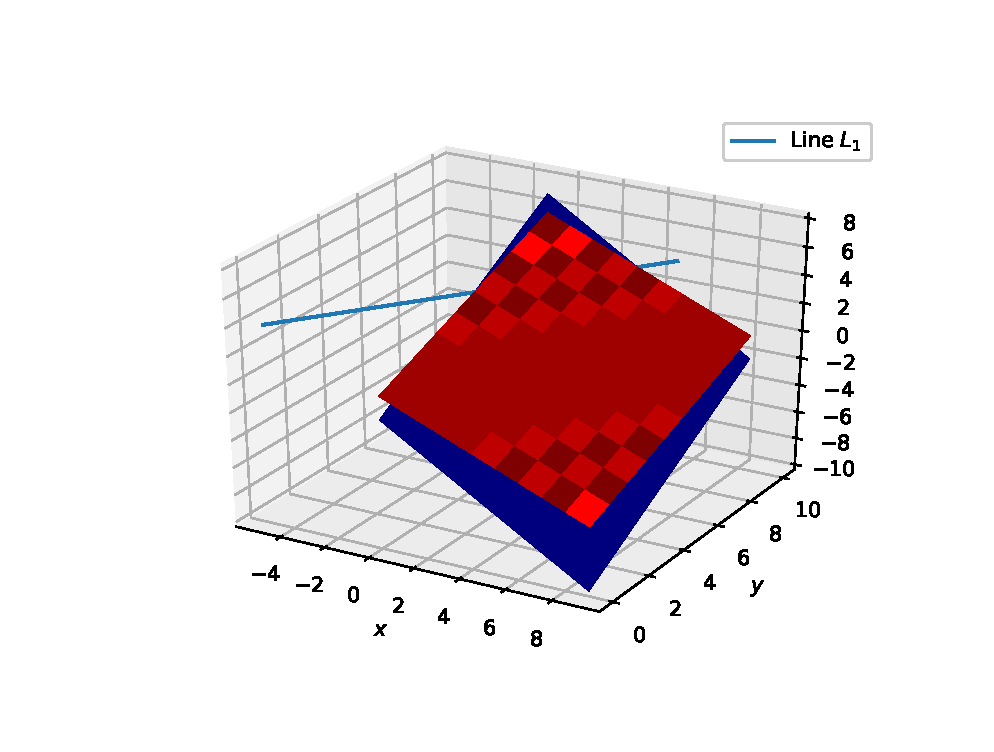
\includegraphics[width=\columnwidth]{./3d/figs/1.1.eps}
\caption{}
\label{fig:1.1}
\end{figure}

\item $L_2$ is the intersection of the planes
\begin{align}
\myvec{1 & 2 & -1}\vec{x} &= 3
\\
\myvec{3 & -1 & 2}\vec{x} &= 1
\end{align}
Show that its equation is
%
\begin{align}
\vec{x} = \frac{1}{7}\myvec{ 5 \\ 8 \\ 0} + \lambda_2 \myvec{ -3 \\ 5 \\ 7}
\label{eq:l2}
\end{align}
\item Plot 
$L_2$.
\\
\solution The following code generates Fig. \ref{fig:1.2}.
\begin{lstlisting}
 
codes/3d/1.2.py
\end{lstlisting}
\begin{figure}[!ht]
\centering
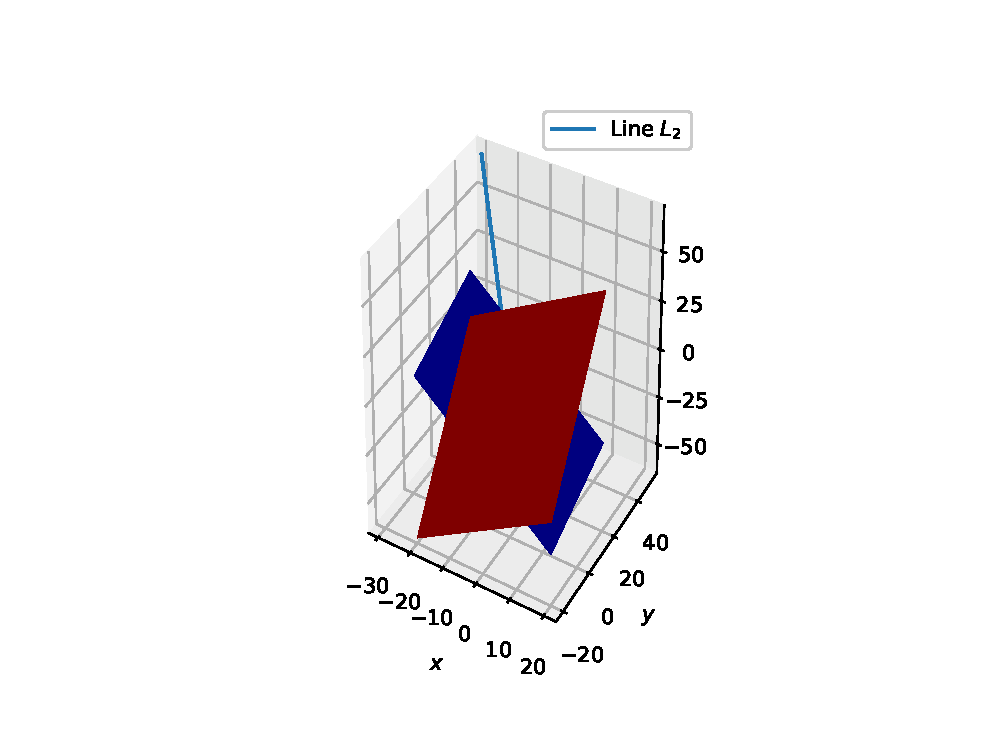
\includegraphics[width=\columnwidth]{./3d/figs/1.2.eps}
\caption{}
\label{fig:1.2}
\end{figure}

\item Do $L_1$ and $L_2$ intersect? If so, find their point of intersection $P$.
\\
\solution From \eqref{eq:l1},\eqref{eq:l2}, the point of intersection is given by
\begin{align}
\label{eq:l1l2pt}
\vec{x} = \frac{1}{7}\myvec{ 5 \\ 8 \\ 0} + \lambda_2 \myvec{ -3 \\ 5 \\ 7} &= \myvec{ 
-5 \\ 0 \\ 4} + \lambda_1 \myvec{ 1 \\ 1 \\ 0}
\\
\implies 
\myvec{1 &  3 \\ 1 & -5 \\ 0 & -7}\vec{\Lambda} &= \frac{1}{7}\myvec{40 \\ 8 \\ -28}
\end{align}
This matrix equation can be solved as
\begin{align}
\myvec{1 &  3 & \frac{40}{7}\\ 1 & -5 &\frac{8}{7}\\ 0 & -7 & -4} &\leftrightarrow \myvec{8 &  0 & 
\frac{224}{7}\\ 0 & 1 &\frac{4}{7}\\ 0 & 1 & \frac{4}{7} }
\\
\leftrightarrow \myvec{1 &  0 & 
4\\ 0 & 1 &\frac{4}{7} } &\implies \vec{\Lambda} = \myvec{4\\\frac{4}{7}}
\end{align}
%
Substituting $\lambda_1 = 4$ in \eqref{eq:l1l2pt}
\begin{align}
\vec{x} = \myvec{4 \\ 4 \\ 0} + \myvec{-5 \\ 0 \\ 4} = \myvec{-1\\ 4\\ 4}
\end{align}
\item Plot $P$.
\\
\solution The following code generates Fig. \ref{fig:1.3}.
\begin{lstlisting}
 
codes/3d/1.3.py
\end{lstlisting}
\begin{figure}[!ht]
\centering
\includegraphics[width=\columnwidth]{./3d/figs/1.3.eps}
\caption{}
\label{fig:1.3}
\end{figure}
\end{enumerate}
 
\subsection{Normal to a Plane}
\renewcommand{\theequation}{\theenumi}
\begin{enumerate}[label=\arabic*.,ref=\thesubsection.\theenumi]
\numberwithin{equation}{enumi}
\item The cross product of $\vec{a},\vec{b}$ is defined as
\begin{equation}
\label{eq:cross}
\vec{a}\times \vec{b} = \myvec{0 & -a_3 & a_2 \\ a_3 & 0 & -a_1 \\ -a_2 & a_1 & 0}\myvec{b_1 \\ b_2 \\ b_3}
\end{equation}
From \eqref{eq:l1}, \eqref{eq:l2}, the direction vectors of $L_1$ and $L_2$ are
\begin{equation}
\myvec{1 \\ 1 \\ 0} \text{ and } \myvec{-3 \\ 5 \\ 7}
\end{equation}
respectively. Find the direction vector of the normal to the plane spanned by $L_1$ and $L_2$.
\\
\solution The desired vector is obtained as
\begin{align}
\myvec{1 \\ 1 \\ 0} \times \myvec{-3 \\ 5 \\ 7} = 
 \myvec{0 & 0 & 1 \\ 0 & 0 & -1 \\ -1 & 1 & 0}\myvec{-3 \\ 5 \\ 7}
= \myvec{7 \\ -7 \\ 8} = \vec{n}
\end{align}
\item Summarize all the above computations through a plot 
\\
\solution The following code generates Fig. \ref{fig:2.1}.
\begin{lstlisting}
wget 
https://github.com/gadepall/school/raw/master/linalg/book/3d/codes/2.1.py
\end{lstlisting}
\begin{figure}[!ht]
\centering
\includegraphics[width=\columnwidth]{./3d/figs/2.1.eps}
\caption{}
\label{fig:2.1}
\end{figure}
\item Find the equation of the plane spanned by $L_1$ and $L_2$.
\\
\solution Let $\vec{x}_0$ be the intersection of $L_1$ and $L_2$.  Then the equation of the plane is
\begin{align}
\brak{\vec{x}-\vec{x}_0}^T\vec{n} &= 0
\\
\implies \vec{x}^T\vec{n} &= \vec{x}_0^T\vec{n}
\\
\implies \vec{x}^T\myvec{7 \\ -7 \\ 8} &= \myvec{-1 & 4 & 4}\myvec{7 \\ -7 \\ 8} =  -3
\end{align}
\item Summarize  the above through a plot. 
\\
\solution The following code generates Fig. \ref{fig:2.2}.
\begin{lstlisting}
wget 
https://github.com/gadepall/school/raw/master/linalg/book/3d/codes/2.2.py
\end{lstlisting}
\begin{figure}[!ht]
\centering
\includegraphics[width=\columnwidth]{./3d/figs/2.2.eps}
\caption{}
\label{fig:2.2}
\end{figure}
\item
Find the distance of the origin from the plane containing the lines $L_1$ and $L_2$.
\\
\solution The distance from the origin to the plane is given by
\begin{equation}
\frac{\abs{\vec{x}_0^T\vec{n}}}{\norm{n}} = \frac{1}{3\sqrt{2}}
\end{equation}
\end{enumerate}
 
\subsection{Projection on a Plane}
\renewcommand{\theequation}{\theenumi}
\begin{enumerate}[label=\arabic*.,ref=\thesubsection.\theenumi]
\item Write down the equations of the polars of the following points with regard to the circle 
\begin{align}
\norm{\vec{x}}^2=6
\end{align}

%\begin{multicols}{2}
\begin{enumerate}
\item
$
\myvec{2\\-1}
$
\item
$
\myvec{3\\4}
$
\end{enumerate}
%\end{multicols}
\item Find the poles of the following lines with regard to the circle 
\begin{align}
\norm{\vec{x}}=3
\end{align}

\begin{enumerate}
\item
$
\myvec{3 & 4}\vec{x}=7
$
\item
$
\myvec{5 & -1}\vec{x}+6=0
$
\end{enumerate}
and verify that the polar of their point of intersection is the line joining their poles.
\item Show that the points $\myvec{4\\-2}$, $\myvec{3\\-6}$ are conjugate with regard to the circle
\begin{align}
\norm{\vec{x}}^2=24
\end{align}
\item Prove that the lines 
\begin{align}
\myvec{5 & 3}\vec{x}=40
\\
\myvec{7 & -5}\vec{x}=10
\end{align}
are conjugate with regard to the circle
\begin{align}
\norm{\vec{x}}^2=20
\end{align}
\item Find the polar of the point $\myvec{5\\4}$ with regard to the circle
\begin{align}
\vec{x}^T\vec{x}-\myvec{4 & 3}\vec{x}-8 = 0
\end{align}
\item Find the pole of 
\begin{align}
\myvec{l & m}\vec{x}+n = 0
\end{align}
with regard to
\begin{enumerate}
\item
$
\norm{\vec{x}}=a
$
\item
$
\vec{x}^T\vec{x}+2\myvec{g & f}\vec{x}+c = 0
$

\end{enumerate}
\item Prove that if two lines at right angles are conjugate with regard to a circle one of them must pass through the centre.
\item Prove that, if the chords of contact of pairs of tangents to a circle from $\vec{P}$ and $\vec{Q}$ intersect in in $\vec{R}$, then the line joining $\vec{R}$ to
the centre is perpendicular to $PQ$.
\end{enumerate}
 
\subsection{Coplanar vectors}
\renewcommand{\theequation}{\theenumi}
\begin{enumerate}[label=\arabic*.,ref=\thesubsection.\theenumi]
\numberwithin{equation}{enumi}
\item If $\vec{u}, \vec{A}, \vec{B}$ are coplanar, show that
\begin{equation}
\vec{u}^T\brak{\vec{A}\times \vec{B}} = 0
\label{eq:coplanar}
\end{equation}
%
\item Find $\vec{A}\times \vec{B}$ given
\begin{align}
\vec{A}=\myvec{2 & 3 & -1}^T
\\
\vec{B}=\myvec{0 & 1 & 1}^T
\end{align}
\solution From \eqref{eq:cross},
\begin{align}
\vec{A}\times \vec{B} &= \myvec{0 & 1& 3 \\ -1 & 0 & -2 \\ -3 & 2 & 0}\myvec{0 \\ 1 \\ 1}
\\
&= \myvec{4 \\ -2 \\ 2}
\label{eq:last_axb}
\end{align}

\item Let $\vec{u}$ be coplanar with $\vec{A}$
%
such that $\vec{u}\perp\vec{A}$ and
\begin{equation}
\vec{u}^T\vec{B} = 24.
\label{eq:uB}
\end{equation}
Find $\norm{\vec{u}}^2$.
\\
\solution From \eqref{eq:last_axb} and the given information,
\begin{align}
\vec{u}^T\myvec{4 & -2 & 2} &=0
\\
\vec{u}^T\myvec{2 & 3 & -1} &=0
\\
\vec{u}^T\myvec{0 & 1 & 1} &=24
\\
\implies \myvec{4 & -2 & 2
\\
2 & 3 & -1
\\
0 & 1 & 1
}\vec{u}
&= \myvec{0 \\ 0 \\ 24}
\\
\implies 
\vec{u} &= 4 \myvec{-1 \\ 2 \\ 4}
\\
\implies \norm{\vec{u}}^2 &= 336
\end{align}
\end{enumerate}
 
\subsection{Orthogonality}
\renewcommand{\theequation}{\theenumi}
\begin{enumerate}[label=\arabic*.,ref=\thesubsection.\theenumi]
\item Find the locus of a point which moves so that the sum of the squares of its distances from the sides of an equilateral triangle
is constant.
\item Find the locus of a point which moves so that the sum of the squares of its distances from $n$ fixed points is constant.
\item Find the locus of a point at which two given circles
subtend equal angles.
\item A circle passes through the four points $\myvec{a\\0}$, $\myvec{b\\0}$, $\myvec{0\\c}$, $\myvec{0\\d}$.  By what relation 
are $a$, $b$, $c$, $d$ connected?  Find the equation of the 
circle and show that the tangent at the point $\myvec{a\\c+d}$ is
\begin{align}
\myvec{a-b & c+d}\vec{x}
-a\brak{a-b}-\brak{c+d}^2=0
\end{align}
\numberwithin{equation}{enumi}
\item Write down the equations of the tangents to the circles
\begin{align}
\vec{x}^T\vec{x}+\myvec{-2a & 0}\vec{x}-5 = 0
\\
\vec{x}^T\vec{x}+\myvec{0 & -2b}\vec{x}-5 = 0
\end{align}
at their points of intersection and verify that they cut at right angles.
\item Find the equation of the tangent to the circle 
\begin{align}
\norm{\vec{x}}=a
\end{align}
 at the point $\myvec{a\cos\theta\\a\sin\theta}$ and show that the length of the
tangent intercepted by the lines 
\begin{align}
\vec{x}^T\myvec{1 & 0\\0 & -1}\vec{x} = 0
\end{align}
is $\pm 2a\sec\theta$.
\item $\vec{A}$ and $\vec{B}$ are two fixed points $\myvec{c\\0}$, $\myvec{-c\\0}$, and $\vec{P}$ moves so that $PA=k.PB$.  Find the locus of $\vec{P}$ and prove that it is 
cut orthogonally by any circle through $\vec{A}$ and $\vec{B}$.
\item Show that the common chord of the circles
\begin{align}
\vec{x}^T\vec{x}-\myvec{6 & 4}\vec{x}+9 = 0
\\
\vec{x}^T\vec{x}-\myvec{8 & 6}\vec{x}+23 = 0
\end{align}
is a diameter of the latter circle and find the angle at which the circles cut.
\item Prove analytically that the tangents to a circle at the ends of a chord are equally inclined to the chord.
\item Prove that for different values of $a$ the equation
\begin{align}
\vec{x}^T\vec{x}+\myvec{-2a\text{cosec}\alpha & 0}\vec{x}+a^2\cot^2\alpha = 0
\end{align}
represents a family of circles touching the lines 
\begin{align}
\myvec{\pm\tan\alpha & 1}\vec{x} = 0
\end{align}
%
Prove also that the locus of the poles of the line 
\begin{align}
\myvec{l & m}\vec{x} = 0
\end{align}
 with regard to the circles is the line
\begin{align}
\myvec{m\sin^2\alpha & l\cos^2\alpha}\vec{x}=0
\end{align}
\item Find the coordinates of the middle point of the chord 
\begin{align}
\myvec{l & m}\vec{x} = 1
\end{align}
of the circle
\begin{align}
\vec{x}^T\vec{x}+2\myvec{g & f}\vec{x}+c = 0
\end{align}
\item Prove that the points of intersection of the line 
\begin{align}
\myvec{l & m}\vec{x} = 1
\end{align}
and the circle
\begin{align}
\vec{x}^T\vec{x}+2\myvec{g & f}\vec{x}+c = 0
\end{align}
subtend a right angle at the origin if
\begin{align}
c\brak{l^2+m^2}+2gl+2fm+2=0
\end{align}
\item Prove that the equation of the circle having for diameter the portion of the line 
\begin{align}
\myvec{\cos\alpha & \sin\alpha}\vec{x} = p
\end{align}
 intercepted by the circle 
\begin{align}
\norm{\vec{x}} = a
\end{align}
 is
\begin{align}
\vec{x}^T\vec{x}-2p\myvec{\cos\alpha & \sin\alpha}\vec{x}+2p^2-a^2 = 0
\end{align}
\item Prove that if a chord of the circle 
\begin{align}
\norm{\vec{x}} = a
\end{align}
subtends a right angle at a fixed point $\vec{x}_1$, the locus of the middle point
of the chord is
\begin{align}
2\vec{x}^T\vec{x}-2\vec{x}_1^T\vec{x}+\norm{\vec{x}_1}^2 - a^2  = 0
\end{align}
\item Prove that the equation of any tangent to the circle
\begin{align}
\norm{\vec{x}-\myvec{a\\b}} = r
\end{align}
may be written in the form
\begin{align}
\myvec{\cos\theta & \sin\theta}\brak{\vec{x}-\myvec{a\\b}} = r
\end{align}
Deduce that the equation of the tangents from $\vec{x}_1$ to the circle is
\begin{multline}
r^2\norm{\vec{x}-\vec{x}_1}^2
\\
 =\sbrak{\cbrak{\vec{x}-\myvec{a\\b}}\myvec{0 & -1\\1 & 0}\cbrak{\vec{x}_1-\myvec{a\\b}}}^2
\end{multline}
\item Prove that the distances of two points from the centre of a circle are proportional to the distance of each point from the polar of the
other.
\item Prove that the tangents to the circles of a coaxal system drawn from a limiting point are bisected by
the radical axis.
\item Show that a common tangent to the two circles is bisected by their radical axis and subtends a right angle at either limiting point.
\item Prove that if a point moves so that the difference of the squares of the tangents from it to two given circles is constant its locus
 is a straight line parallel to the radical axis of the circles.
 \item Prove that the polars of a fixed point with regard to a family of coaxal circles all pass through another fixed point.
 \item The circles
 \begin{align}
\vec{x}^T\vec{x}+\myvec{-2a\sec\alpha & 0}\vec{x}-a^2 = 0
 \\
\vec{x}^T\vec{x}+\myvec{0 & -2a\text{cosec}\alpha}\vec{x}-a^2 = 0
 \end{align}
 where $\alpha$ is a given angle, both cut orthogonally every member of a coaxal family of circles.  Find the radical axis and the limiting
 points of the family.
 \item Prove that, if two points $\vec{P}$, $\vec{Q}$ are conjugate with regard to a circle, the circle on $PQ$ as diameter cuts the first circle orthogonally. 
 \item Prove that if $\vec{P}$, $\vec{Q}$ are conjugate points with regard to a circle, the circles
 with $\vec{P}$, $\vec{Q}$ as centres which cut the given circle orthogonally are orthogonal to one another.
 \item Prove that, if $PQ$ is a diameter of a circle, then $\vec{P}$, $\vec{Q}$ are conjugate points with regard to
 any circle which cuts the given circle orthogonally.
 \item Prove that if $\vec{P}$, $\vec{Q}$ are conjugate points with regard to a circle, the square on $PQ$ is equal to the
 sum of the squares on the tangents from $\vec{P}$, $\vec{Q}$ to the circle.
\renewcommand{\theequation}{\theenumi}
 \item The equation 
 \begin{align}
\vec{x}^T\vec{x}+\myvec{-2g & 0}\vec{x}+2g-5 = 0
 \end{align}
 where $g$ is a variable parameter, represents a family of coaxial circles.  
 Show that the radius of the smallest circle of the family is 2.
 \item Prove that, if perpendiculars are drawn from a fixed point $\vec{P}$ to the polars of $\vec{P}$ with regard to a
 family of coaxial circles, then the locus of the feet of these perpendiculars is a circle whose centre
 lies on the radical axis of the family.
\numberwithin{equation}{enumi}
 \item Prove that, if the points in which the line 
 \begin{align}
\myvec{l & m}\vec{x}+n=0
 \end{align}
meets the circle, 
 \begin{align}
\vec{x}^T\vec{x}+2\myvec{g & f}\vec{x}+c = 0
 \end{align}
 and those in which the line 
 \begin{align}
\myvec{l_1 & m_1}\vec{x}+n_1=0
 \end{align}
 meets 
 \begin{align}
\vec{x}^T\vec{x}+2\myvec{g_1 & f_1}\vec{x}+c_1 = 0
 \end{align}
lie on a circle,
 then 
 \begin{multline}
 2\brak{g-g_1}\brak{mn_1-m_1n}+2\brak{f-f_1}
 \\
 \brak{nl_1-n_1l}+\brak{c-c_1}\brak{lm_1-l_1m}=0
 \end{multline}
 \item Show that, if a diameter of a circle is the portion of the line 
 \begin{align}
\myvec{l & m}\vec{x}=1
 \end{align}
intercepted by the lines 
 \begin{align}
\vec{x}^T\myvec{a & h\\h & b}\vec{x} = 0
 \end{align}
 then the 
 equation of the circle is
 \begin{multline}
\brak{am^2-2hlm+bl^2}\vec{x}^T\vec{x}
\\
+2\myvec{\brak{hm-bl} & \brak{hl-am}}\vec{x}+ a+b = 0
 \end{multline}
\item Prove that, as $k$ varies, the equation
 \begin{align}
\vec{x}^T\vec{x}+2\myvec{a & b}\vec{x}+c + 2k\cbrak{\myvec{a & -b}\vec{x}+1}= 0
 \end{align}
 represents a system of coaxial circles.  Also prove that the orthogonal system is given by
 \begin{align}
\vec{x}^T\vec{x}+\myvec{\frac{c+2}{2a} & \frac{c-2}{2b}}\vec{x}+h\cbrak{\myvec{\frac{1}{2a}&\frac{1}{2b}}\vec{x} + 1} = 0
 \end{align}
 where $h$ is a variable parameter.
\end{enumerate}
 
\subsection{Least Squares}
\renewcommand{\theequation}{\theenumi}
\begin{enumerate}[label=\arabic*.,ref=\thesubsection.\theenumi]
\numberwithin{equation}{enumi}

\item Let
\begin{align}
L_1: \quad \vec{x} &= \myvec{1 \\ 0 \\ 0} + \lambda_1 \myvec{-1 \\ 2 \\ 2}
\\
L_2: \quad \vec{x} &=  \lambda_1 \myvec{2 \\-1 \\ 2}
\end{align}
%
Given that  $L_3 \perp L_1, L_3 \perp L_2$, find $L_3$.
\\
\solution Let 
\begin{align}
L_3: \quad \vec{x} &= \vec{c}+ \lambda \vec{m}_3
\end{align}
% 
Then
\begin{align}
\myvec{-1 & 2 & 2
\\
2 &-1 & 2}\vec{m}_3 = \vec{0}
\end{align}
%
Row reducing the coefficient matrix,
\begin{align}
\myvec{-1 & 2 & 2
\\
2 &-1 & 2} &\leftrightarrow 
\myvec{1 & -2 & -2
\\
0 &1 & 2} 
\\
\leftrightarrow 
\myvec{1 & 0 & 2
\\
0 &1 & 2} 
& \implies \vec{m}_3 = \myvec{2 \\ 2 \\ -1}
\end{align}
%
Also, $L_1\perp L_2$, but $L_1 \cup L_2 = \phi$. The given information can be summarized as
\begin{align}
\label{eq:12-given1}
L_1: \quad \vec{x} &= \vec{c}_1 + \lambda_1 \vec{m}_1
\\
L_2: \quad \vec{x} &=  \lambda_2 \vec{m}_2
\\
L_3: \quad \vec{x} &= \vec{c}_3 + \lambda \vec{m}_3
\label{eq:12-given3}
\end{align}
%
where
\begin{align}
\label{eq:12-given12}
\vec{c}_1 = \myvec{1 \\ 0 \\ 0}, \vec{m}_1=  \myvec{-1 \\ 2 \\ 2},
\vec{m}_2 = \myvec{2 \\-1 \\ 2}
\end{align}
The objective is to find $\vec{c}_3$.  Since $L_1 \cup L_3 \ne \phi, L_2 \cup L_3 \ne \phi$, from \eqref{eq:12-given1}-\eqref{eq:12-given3},
\begin{align}
\label{eq:12-isect13}
\vec{c}_1 + \lambda_1 \vec{m}_1 &= \vec{c}_3 + \lambda_3 \vec{m}_3
\\
  \lambda_2 \vec{m}_2 &= \vec{c}_3 + \lambda_4 \vec{m}_3
\label{eq:12-isect23}
\end{align}
%
Using the fact that $L_1\perp L_2\perp L_3$, \eqref{eq:12-isect13}-\eqref{eq:12-isect23} can be expressed as
\begin{align}
%\label{eq:12-isect13}
\vec{m}_1^T\vec{c}_1 + \lambda_1 \norm{\vec{m}}_1^2 &= \vec{m}_1^T\vec{c}_3 
\\
\vec{m}_2^T\vec{c}_1  &= \vec{m}_2^T\vec{c}_3 
\\
\vec{m}_3^T\vec{c}_1  &= \vec{m}_3^T\vec{c}_3 + \lambda_3 \norm{\vec{m}_3}^2
\\
0 &= \vec{m}_1^T\vec{c}_3 
\\
  \lambda_2 \norm{\vec{m}_2}^2 &= \vec{m}_2^T\vec{c}_3 
\\
0 &= \vec{m}_3^T\vec{c}_3  + \lambda_4 \norm{\vec{m}_3}^2
%\label{eq:12-isect23}
\end{align}
%
Simplifying the above, 
\begin{align}
 \lambda_1  &= -\frac{\vec{m}_1^T\vec{c}_1}{\norm{\vec{m}}_1^2} = \frac{1}{9}
\\
 \lambda_2  &= \frac{\vec{m}_2^T\vec{c}_1}{\norm{\vec{m}}_2^2} =\frac{2}{9}
\end{align}
%
Substituting in \eqref{eq:12-isect13} and \eqref{eq:12-isect23},
\begin{align}
L_3: \quad \vec{x} &= \frac{2}{9}\myvec{4 \\ 1 \\ 1} + \lambda_3\myvec{2 \\ 2 \\ -1} \text{ or}
\\
L_3: \quad \vec{x} &= \frac{2}{9}\myvec{2 \\-1 \\ 2} + \lambda_3\myvec{2 \\ 2 \\ -1}
\end{align}
%
The key concept in this question is that orthogonality of $L_1$ and $L_2$ doesnot mean that they intersect.  They are skew lines.
\end{enumerate}
%

 
\subsection{Singular Value Decomposition}
\renewcommand{\theequation}{\theenumi}
\begin{enumerate}[label=\arabic*.,ref=\thesubsection.\theenumi]
\numberwithin{equation}{enumi}
\item Let $\mbf{v}_1,\mbf{v}_2$ be the columns of $\mbf{C} = \vec{X}^T\vec{X}$.

\item
	Obtain $\mbf{u}_1,\mbf{u}_2$ from $\mbf{v}_1,\mbf{v}_2$ through the following equations. 
	%
\begin{align}
\mbf{u}_1&= \frac{\mbf{v}_1}{\norm{\mbf{v}_1}}
\\
\hat{\mbf{u}}_2 &= \mbf{v}_2 - \brak{\mbf{v}_2,\mbf{u}_1}\mbf{u}_1
\\
\mbf{u}_2 &= \frac{\hat{\mbf{u}}_2}{\norm{\hat{\mbf{u}}_2}}
\end{align}
	%
	This procedure is known as Gram-Schmidt orthogonalization.


\item
Stack the vectors $\mbf{u}_1,\mbf{u}_2$ in columns to obtain the matrix $\mbf{Q}$.  Show that $\mbf{Q}$ is orthogonal.  


\item
	From the Gram-Schmidt process, show that $\mbf{C}=\mbf{Q}\mbf{R}$, where $\mbf{R}$ is an upper triangular matrix.  This is known as the $\mbf{Q}-\mbf{R}$ decomposition.  


\item
	Find an orthonormal basis for $\vec{X}^T\vec{X}$ comprising of the eigenvectors.  Stack these orthonormal eigenvectors in a matrix $\mbf{V}$. This is known as {\em Orthogonal Diagonalization}.  

\item
	Find the singular values of $\vec{X}^T\vec{X}$.  The singular values are obtained by taking the square roots of its eigenvalues.  

\item
	Stack the singular values of $\vec{X}^T\vec{X}$ diagonally to obtain a matrix $\mbf{\Sigma}$.


\item
	Obtain the matrix $\vec{X}\mbf{V}$.  Verify if the columns of this matrix are orthogonal.


\item
	Extend the columns of $\vec{X}\mbf{V}$ if necessary, to obtain an orthogonal matrix $\mbf{U}$.


\item
	Find $\mbf{U}\mbf{\Sigma}\mbf{V}^T$.  Comment.


\end{enumerate}

 
%
\section{Optimization}
\subsection{Convex Functions}
\renewcommand{\theequation}{\theenumi}
%\subsection{Problem}

\begin{enumerate}[label=\arabic*.,ref=\thesection.\theenumi]
\numberwithin{equation}{enumi}

\item
The following python script plots 
%
\begin{align}
f(\lambda) = a\lambda^2 + b\lambda + d
\label{eq:parab}
\end{align}
%
for 
\begin{align}
a &= \norm{\vec{m}}^2 > 0
\\
b &= \vec{m}^T\brak{\vec{A} -\vec{P}} 
\\
c &= \norm{\vec{A} -\vec{P}}^2
\end{align}
where $\vec{A}$ is the intercept of the line $L$ in \eqref{eq:opt_line_nor}
on the x-axis and the points
\begin{align}
\vec{U} &= \myvec{\lambda_1\\f(\lambda_1)}, 
\vec{V} = \myvec{\lambda_2\\f(\lambda_2)}
\\
\vec{X} &= \myvec{t \lambda_1 + \brak{1-t}\lambda_2 \\ f\sbrak{t \lambda_1 + \brak{1-t}\lambda_2}},
\\
\vec{Y} &= \myvec{t \lambda_1 + \brak{1-t}\lambda_2 \\ t f\brak{\lambda_1} + \brak{1-t}f\brak{\lambda_2}}
\end{align}
%
for 
\begin{align}
\lambda_1 = -3, 
\lambda_2 = 4, 
t = 0.3
\end{align}
in Fig. \ref{fig:conv_def}. Geometrically, this means that any point $\vec{Y}$ between the points $\vec{U}, \vec{V}$ on the line $UV$ is always above the point $\vec{X}$ on the curve $f(\lambda)$.
Such a  function $f$ is defined to be {\em convex} function 
%
\begin{lstlisting}
codes/optimization/1.2.py
\end{lstlisting}
%
%%
\begin{figure}[!ht]
\centering
\includegraphics[width=\columnwidth]{./figs/convex.eps}
\caption{ $f(\lambda)$ versus $\lambda$}.
\label{fig:conv_def}	
\end{figure}
%
\item Show that
%
\begin{align}
\label{eq:convex_def}
f\sbrak{t \lambda_1 + \brak{1-t}\lambda_2} \leq 
t f\brak{\lambda_1} + \brak{1-t}f\brak{\lambda_2}
\end{align}
%
for $\quad 0 < t < 1$.  This is true for any convex function.
%
\item Show that 
%
\begin{equation}
\eqref{eq:convex_def} \quad \implies f^{(2)}(\lambda) > 0
\end{equation}
%
\item Show that a covex function has a unique minimum.
%
\end{enumerate}
%

\subsection{More on Convexity}
\renewcommand{\theequation}{\theenumi}
%\subsection{Problem}

\begin{enumerate}[label=\arabic*.,ref=\thesubsection.\theenumi]
\numberwithin{equation}{enumi}
%
%
\item Consider the optimization problem
\begin{align}
\label{eq:opt_def}
\max_{z} \frac{1}{\abs{z-1}}
\\
s.t. \quad \abs{z-2 + \j} \ge \sqrt{5}
\end{align}
%
Show that it can be reframed as
\begin{align}
\label{eq:opt_rev}
\min_{\vec{x}} \,\norm{\vec{x} - \vec{c}_1}^2
\\
 s.t. \quad  \norm{\vec{x} - \vec{c}_2}^2 \ge 5
%\min_{z} \abs{z-1}
%\\
% s.t. \quad \abs{z-2 + \j} \ge \sqrt{5}
\end{align}
%
where
\begin{align}
z &= \vec{x} = \myvec{x_1 \\ x_2},
%\\
\vec{c}_1 = \myvec{1 \\ 0},
%\\
\vec{c}_2 = \myvec{2 \\ -1}
\end{align}

%
%
%Then, 
%\begin{align}
%\Gamma: \abs{z-1} = \norm{\vec{x} - \vec{c}_1}^2,
%\end{align}
%where 
%\begin{align}
%\end{align}
%Similarly, 
%\begin{align}
%\Omega:\abs{z-2+\j} = \norm{\vec{x} - \vec{c}_2}^2,
%\end{align}
%where 
%\begin{align}
%\end{align}
%
%Let 
%\begin{align}
% \abs{z_0-1} = r
%\end{align}
%
%
\item Explain the optimization problem with a figure.
\\
\solution
Fig. \ref{fig:2019_1} explains \eqref{eq:opt_rev}
where $z_0$ is the set of points comprising of the intersection of the 
smallest circle $\Gamma:$ with the largest circle $\Omega: r_2 \ge 
\sqrt{5}$ 
with radii 
$r_1$ and 
$r_2 \ge \sqrt{5}$ respectively.
\begin{figure}[!ht]
\centering
\includegraphics[width=\columnwidth]{./optimization/figs/2019_1_1.eps}
\caption{}
\label{fig:2019_1}
\end{figure}
%
\item Obtain the Lagrangian.
\\
\solution
The Lagrangian is 
\begin{align}
L \brak{\vec{x},\lambda} = \norm{\vec{x} - \vec{c}_1}^2 - \lambda 
\cbrak{\norm{\vec{x} - \vec{c}_2}^2-r_2^2}
\end{align}
\item Use the KKT conditions to obtain the minima.
\\
\solution
From the KKT conditions, 
\begin{align}
\frac{\partial L \brak{\vec{x},\lambda}}{\partial \vec{x}} &= 0
\\
\implies {\vec{x} - \vec{c}_1} - \lambda \brak{\vec{x} - \vec{c}_2} &= 0
\\
\implies \vec{x}  = \frac{\vec{c}_1 -\lambda  \vec{c}_2}{1-\lambda } &
\label{eq:opt_xlam}
\end{align}
%
and 
\begin{align}
\frac{\partial L \brak{\vec{x},\lambda}}{\partial \lambda} &= 0
\\
\implies \norm{\vec{x} - \vec{c}_2}^2-r_2^2 &= 0
\label{eq:opt_xnorm}
\end{align}
Substituting from \eqref{eq:opt_xlam} in \eqref{eq:opt_xnorm},
\begin{align}
\norm{\frac{\vec{c}_1 -\lambda  \vec{c}_2}{1-\lambda } - \vec{c}_2}^2-r_2^2 &= 0
\\
\implies \lambda = 1\pm \frac{\norm{\vec{c}_1 - \vec{c}_2}}{r_2}&
\\
= 1 \pm \sqrt{\frac{2}{5}}
%\label{eq:opt_xnorm}
\end{align}
Fig. \ref{fig:2019_1_2} plots $\Gamma$ for 
\begin{align}
\lambda = 1 - \sqrt{\frac{2}{5}}
\end{align}
\item If the maximum value is obtained at $z_0$, find the principal argument of
\begin{align}
\frac{4 - z_0-\bar{z}_0}{z_0-\bar{z}_0+2\j}
\end{align}
\\
\solution 
From \eqref{eq:opt_xlam},
\begin{align}
 \vec{x}_0  &= \frac{\vec{c}_1 -\lambda  \vec{c}_2}{1-\lambda } 
\\
\implies z_0 &= \frac{1}{1-\lambda}\brak{1-2\lambda + \j \lambda }
\\
\text{or, }\arg \frac{4 - z_0-\bar{z}_0}{z_0-\bar{z}_0+2\j} &= \frac{2 - \Re\cbrak{z_0}}{\j\brak{\Im\cbrak{z_0}+1}}
\\
&=\frac{2\brak{1-\lambda}-\brak{1-2\lambda}}{\j} 
\\
&= -\j
\end{align}
%
Thus, the principal argument is $-\frac{\pi}{2}$.
\begin{figure}[!ht]
\centering
\includegraphics[width=\columnwidth]{./optimization/figs/2019_1_2.eps}
\caption{}
\label{fig:2019_1_2}
\end{figure}

%\begin{enumerate}[label=\theenumi.\arabic*
%,ref=\thesection.\theenumi]
\item Show that the set 
\begin{align}
D = \cbrak{\vec{x}:\norm{\vec{x}-\vec{C}_2} \ge r_2}, r_2 > 0
\end{align}
%
is nonconvex.
\\
\solution Let $\vec{x}_1 \in D$ and 
\begin{align}
\vec{x}_2 = 2\vec{C}_2-\vec{x}_1
\end{align}
Then 
\begin{align}
\norm{\vec{x}_2-\vec{C}_2} &= \norm{\vec{C}_2-\vec{x}_1} \ge r_2
\\
\implies \vec{x}_2 &\in D.
\end{align}
Suppose 
\begin{align}
\vec{x} = \theta\vec{x}_1+\brak{1-\theta}\vec{x}_2
\end{align}
For $\theta = \frac{1}{2}$,
\begin{align}
\vec{x} &= \vec{C}_2
\\
\implies \norm{\vec{x}-\vec{C}_2} &= 0,
\\
\text{or, } \vec{x} &\notin D
\end{align}
Thus, by definition, $D$ is not a convex set.
\end{enumerate}



\subsection{Gradient Descent Method}
\renewcommand{\theequation}{\theenumi}
\begin{enumerate}[label=\arabic*.,ref=\thesection.\theenumi]
\numberwithin{equation}{enumi}
%\item Consider the problem of finding the square root of a number $c$.  This can be expressed as the equation
%%
%\begin{equation}
%\label{eq:root}
%x^2 -c= 0
%\end{equation}
%%
%
%\item
%Sketch the function for different values of $c$
%%
%\begin{equation}
%f(x)= x^{3}-3xc
%\end{equation}
%%
%and comment upon its convexity.
%
%\item
%Show that \eqref{eq:root} results from
%\begin{align}
%\min_{x}f(x)= x^{3}-3xc
%\end{align}

\item
Find a numerical solution for \eqref{eq:parab}

%
%\begin{align}
%f(\lambda) = a\lambda^2 + b\lambda + d
%\end{align}
%
%\eqref{eq:root}.
%\\
\solution
A numerical solution for \eqref{eq:root} is obtained as
%
\begin{align}
\lambda_{n+1}&=\lambda_{n}-\mu f^{\prime}\brak{\lambda_n}
\\
&=\lambda_{n} -\mu \brak{2a\lambda_n+b}
\label{eq:gradient}
\end{align}

%\begin{align}
%x_{n+1}&=x_{n}-{\frac {f(x_{n})}{f^{\prime}(x_{n})}}
%\\
%&=x_{n} -\frac{x^2_{n}-c}{2x_n} 
%\\
%&=\frac{1}{2}\sbrak{x_{n} +\frac{c}{x_n} }
%\label{eq:newton}
%\end{align}
%
where $\lambda_0$ is an inital guess.
%
\item
Write a program to implement \eqref{eq:gradient}.
%
\\
\solution Download and execute
\begin{lstlisting}
codes/optimization/gd.py
\end{lstlisting}
%
\item Find a closed form solution for \eqref{eq:gradient} using the one sided Z transform.
%
\item Find the condition for which \eqref{eq:gradient} converges, i.e.
\begin{align}
\lim_{n \to \infty}\abs{\lambda_{n+1}-\lambda_n} = 0
\end{align}
\end{enumerate}


\subsection{Semi-definite Programming}
\renewcommand{\theequation}{\theenumi}
\begin{enumerate}[label=\arabic*.,ref=\thesection.\theenumi]
\numberwithin{equation}{enumi}

%\item An apache helicopter of the enemy is flying along the curve given by 
%	\label{prob:dist_pt_parab_sdp}
%\begin{align}
%\label{eq:dist_pt_parab_sdp}
%y = x^2 +7
%\end{align}
%%
%A soldier, placed at 
%\begin{align}
%\vec{P} = \myvec{3\\7}.  
%\end{align}
%%
%wants to shoot the heicopter when it is nearest to him.  Express this as an optimization problem.
\item
	\label{prob:dist_pt_parab_sdp}
Express the problem of 
finding the point on the curve 
\begin{align}
\label{eq:dist_pt_parab_sdp}
x^2 = 2y
\end{align}
%
nearest to the point 
\begin{align}
\vec{P} = \myvec{0\\5}.  
\end{align}
%
as an optimization problem.
\\
\solution The given problem can be expressed as
%
\begin{align}
\label{eq:qp_dist_pt_parab_sdp_qp}
\min_{\vec{x}}\vec{x}^T\vec{Q}_0\vec{x}+\vec{q}_0^T\vec{x}+c_0
\\
\text{s.t. }\vec{x}^T\vec{Q}_1\vec{x} + \vec{q}_1^T\vec{x} +c_1 \le 0
\end{align}
%
%where $\vec{V} \succeq 0$.
%\begin{align}
%\label{eq:qp_dist_pt_parab_sdp}
%\begin{split}
%\min_{\vec{x}}\vec{X}^T\myvec{\vec{I} & \vec{0} \\ \vec{0} & \vec{0}}\vec{X}-2\myvec{\vec{P}^T & \vec{0}}\vec{X}+\norm{\vec{P}}^2
%\\
%\text{s.t. }\vec{x}^T\vec{V}\vec{x} + \vec{u}^T\vec{x}  = 0
%\end{split}
%\end{align}
%
where
%
\begin{align}
\vec{Q}_0 &= \vec{I}, \vec{Q}_1 = \myvec{1 & 0\\0 & 0}
\\
\vec{q}_0 &=-2\vec{P}, \vec{q}_1 = -2\myvec{0 \\ 1}
\\
c_0 &= \norm{\vec{P}}^2, c_1 = 0
\end{align}
%\item Show that the constraint in 	
%%\label{prob:dist_pt_parab_sdp}
%\eqref{eq:qp_dist_pt_parab_sdp} is nonconvex.
%
\item Show that \eqref{eq:qp_dist_pt_parab_sdp_qp} is equivalent to
\begin{align}
\label{eq:qp_dist_pt_parab_sdp_conv}
\begin{split}
\min_{\vec{x},\theta}\theta
\\
\text{s.t. } \myvec{\vec{I} & \vec{M}_0\vec{x} \\ \vec{x}^T\vec{M}_0^T & -c_0-q_0^T\vec{x}+\theta} &\succeq 0
\\
\myvec{\vec{I} & \vec{M}_1\vec{x} \\ \vec{x}^T\vec{M}_1^T & -c_1-q_1^T\vec{x}} &\succeq 0
\end{split}
\end{align}
%
%\item Show that the following {\em relaxation} makes \eqref{eq:qp_dist_pt_parab_sdp} a convex optimization problem.
%%
%\begin{align}
%\label{eq:qp_dist_pt_parab_sdp_conv}
%\min_{\vec{x}}\brak{\vec{x}-\vec{P}}^T\brak{\vec{x}-\vec{P}}
%\\
%\text{s.t. }\vec{x}^T\vec{V}\vec{x} + \vec{u}^T\vec{x}  \le 0
%\end{align}
%
where
\begin{align}
\vec{Q}_i = \vec{M}_i^T\vec{M}_i, i = 0, 1
\end{align}
%
\item Solve \eqref{eq:qp_dist_pt_parab_sdp_conv} using cvxpy.
\item Graphically verify the solution to Problem \ref{prob:dist_pt_parab_sdp}. 
%\\
%\solution  The following code yields the minimum distance as 2.236 and the nearest point on the curve as
%%
%\begin{align}
%\vec{Q} &= \myvec{1\\8}
%\end{align}
%
%\begin{lstlisting}
%codes/qp_cvx.py
%\end{lstlisting}

\item Solve \eqref{eq:qp_dist_pt_parab_sdp_qp} using the method of Lagrange multipliers.
%by drawing a figure.
%\\
%\solution 
%The following code plots Fig. \label{fig:qp_parab_sdp}
%%	
%\begin{lstlisting}
%codes/qp_parab.py
%\end{lstlisting}
%
%%
%\begin{figure}[!ht]
%\centering
%\includegraphics[width=\columnwidth]{./figs/qp_parab.eps}
%\caption{ $\vec{Q}$ is closest to $\vec{P}$}.
%\label{fig:qp_parab_sdp}
%\end{figure}
%
%\item Frame 	
% as an optimization problem.
%\label{prob:qp_dist_pt_parab}
%\\
%
%\solution 
%From \eqref{eq2_1_line} and \eqref{eq2_1_circ}, 
%%
%\begin{align}
%r^2 & = (x_1-8)^2 + (3- x_1)^2 \\
%&= 2 x_1^2 - 22 x_1 + 73 \\
%\Rightarrow r^2 &= \frac{\brak{2x_1-11}^2 + 5^2}{2}
%\end{align}
%%
%which is minium when $x_1 = \frac{11}{2}, x_2 = \frac{7}{2}$.  The minimum value is $\frac{25}{2}$ and 
%the radius $r = \frac{5}{\sqrt{2}}$.
%	
%\begin{lstlisting}
%codes/optimization/lagmul.py
%\end{lstlisting}
%\item Solve \eqref{eq:qp_dist_pt_parab_sdp_conv} using gradient descent.
%
\end{enumerate}

\subsection{Linear Programming}
\renewcommand{\theequation}{\theenumi}
\begin{enumerate}[label=\arabic*.,ref=\thesubsection.\theenumi]
\numberwithin{equation}{enumi}
	
\item
\label{ch1_lp1}
	Graphically obtain a solution to the following 
	\begin{align}
\max_{\mbf{x}}	6x_1 + 5x_2
	\end{align}
	with constraints
	\begin{align}
	x_1 + x_2 &\leq 5\\
	3x_1 + 2x_2 &\leq 12\\
	\text{ where } x_1,x_2 &\geq 0
	\end{align}

%
\solution
The following program plots the solution in Fig. \ref{fig.4.1}
%	
\begin{lstlisting}
codes/optimization/4.1.py
\end{lstlisting}

%
\begin{figure}[!ht]
\centering
\includegraphics[width=\columnwidth]{./optimization/figs/4.1.eps}
\caption{ The cost function intersects with the two constraints at $\mbf{x} = \brak{2,3}$. }
\label{fig.4.1}	
\end{figure}
%
\item
	Now use {\em cvxpy} to obtain a solution to problem \ref{ch1_lp1}.

\solution
The given problem is expressed as follows
%
\begin{align}
\min_{\mbf{x}}	\mbf{c}^{T}\mbf{x}\quad s.t.
\\
\mbf{A}\mbf{x} \preceq \mbf{b}
\end{align}
%
where
%
\begin{equation}
\mbf{c}
=
\begin{pmatrix}
-6
\\
-5
\end{pmatrix},
\mbf{A} = 
\begin{pmatrix}
1 & 1
\\
3 & 2
\\
-1 & 0
\\
0 & -1
\end{pmatrix},
\mbf{b}
= 
\begin{pmatrix}
5
\\
12
\\
0
\\
0 
\end{pmatrix}
\end{equation}
%	
The desired solution is then obtained using the following program.
%\begin{lstlisting}
%codes/optimization/4.2.py
%\end{lstlisting}
%
%
%\item
%Repeat the previous exercise using {\em cvxpy}
%
%\solution
\begin{lstlisting}
codes/optimization/4.2-cvx.py
\end{lstlisting}

\item
	Verify your solution to the above problem using the method of Lagrange multipliers.

%
\item
	 Maximise $5x_1 + 3x_2$ w.r.t the constraints
	 \begin{align}
	 x_1 + x_2 &\leq 2 \nonumber\\
	 5x_1 + 2x_2 &\leq 10 \nonumber\\
	 3x_1 + 8x_2 &\leq 12 \nonumber\\
	 \text{ where } x_1,x_2 &\geq 0 \nonumber
	 \end{align}	

\end{enumerate}
%

\subsection{Exercises}
\renewcommand{\theequation}{\theenumi}
\begin{enumerate}[label=\arabic*.,ref=\thesubsection.\theenumi]
\numberwithin{equation}{enumi}

\item Let $\vec{P}$ be the point on the parabola
\begin{equation}
\label{eq:parab_circ_parab}
\vec{x}^T\myvec{0 & 0 \\ 0 & 1}\vec{x} -\myvec{8 & 0 }\vec{x} 
 = 0
\end{equation}
which is at a minimum distance from the centre $\vec{C}$ of the circle
\begin{equation}
\label{eq:parab_circ_circ}
\vec{x}^T\vec{x} +\myvec{0 & 12 }\vec{x} 
 = 1 
\end{equation} 
Find the equation of the circle passing through $\vec{C}$ and having its centre at $\vec{P}$. 
\item Let $\vec{P}$ 
be a point on the parabola
\begin{equation}
\vec{x}^T\myvec{1 & 0 \\ 0 & 0}\vec{x} +\myvec{0 & 4 }\vec{x} 
 = 0
\end{equation}
%%
Given that the distance of $\vec{P}$ from the centre of the circle
\begin{equation}
\vec{x}^T\vec{x} +\myvec{6 \\ 0 }\vec{x} + 8 = 0
\end{equation}
%
is minimum.  Find the equation of the tangent to the parabola at $\vec{P}$.
\item Find the eccentricity of the hyperbola whose length of the latus rectum is equal to 8 and the length of 
its conjugate axis is equal to half the distance between its foci. 
\item $\vec{P}$ and $\vec{Q}$ are two distinct points on the parabola
\begin{equation}
\vec{x}^T\myvec{0 & 0 \\ 0 & 1}\vec{x} -\myvec{4 & 0 }\vec{x} 
 = 0
\end{equation}
with parameters $t$ and $t_1$ respectively.  If the normal at $\vec{P} $ passes through $\vec{Q}$, then find 
the minimum value of $t_1^2$ using a descent algorithm.
\item A tangent at a point on the ellipse 
\begin{equation}
\vec{x}^TV\vec{x} =51
\end{equation}
%
where
\begin{equation}
V = \myvec{3 & 0 \\ 0 & 27}
\end{equation}
%
meets the coordinate axes at  $\vec{A}$  and  $\vec{B}$.  If   $\vec{O}$  be the origin, find the minimum area 
of $\triangle OAB$.
\item Find the shortest distance between the line 
\begin{equation}
\myvec{1 & -1 }\vec{x}  =0
\end{equation}
%
and the curve
\begin{equation}
\vec{x}^T\myvec{0 & 0 \\ 0 & 1}\vec{x} - \myvec{1 & 0}\vec{x} + 2 =0
\end{equation}
\item Let $S$ be the set of all complex numbers $z$ satisfying $\abs{z-2+\j} \ge \sqrt{5}$. If the complex number $z_0$ is such that $\frac{1}{\abs{z_0-1}}$ is the maximum of the set $\cbrak{\frac{1}{\abs{z-1}}: z \in S}$, find the principal argument of 
\begin{align}
\frac{4-z_0-\bar{z}_0}{z_0-\bar{z}_0+2\j}
\end{align}
\item Let $\omega \ne 1$ be a cube root of unity. Find the minimum of the set
\begin{align}
\abs{a+b\omega+c\omega^2}, 
\end{align}
%
where $a,b,c$ are distinct nonzero integers.
\item Let 
\begin{align}
\label{eq:mat_def}
\vec{M} = \myvec{\sin^4\theta & -1-\sin^2\theta \\ 1+ \cos^2\theta & \cos^4\theta} = \alpha\vec{I} + \beta \vec{M}^{-1}
\end{align}
where $\alpha, \beta$ are real functions of $\theta$ and $\vec{I}$ is the identity matrix. If 
\begin{align}
\alpha^{*} &= \min_{\theta}\alpha\brak{\theta}
\\
\beta^{*} &= \min_{\theta}\beta\brak{\theta}, 
\end{align}
find $\alpha^{*} + \beta^{*}$.
\item Find the minimum value of 
\begin{align}
\cos \brak{P+Q}
\cos \brak{Q+R}
\cos \brak{R+P}
\end{align}
%
in $\triangle PQR$.
\item Find the minimum value of $\alpha$ for which 
\begin{align}
4\alpha x^2 + \frac{1}{x} \ge 1, x > 0.
\end{align}
\item Let 
\begin{align}
S = S_1\cap S_2\cap S_3,
\end{align}
%
where
\begin{align}
S_1 &= \cbrak{z\in C: \abs{z}< 4}
\\
S_2 &= \cbrak{z\in C: \Im\sbrak{\frac{z-1+\j\sqrt{3}}{1-\j\sqrt{3}}}},
\\
S_3 &= \cbrak{z\in C: \Re\brak{z} > 0}
\end{align}
Find
\begin{align}
\min_{z\in S}\abs{1-3\j-z}
\end{align}
\item A line 
\begin{align}
L: \myvec{m -1}\vec{x} = -3
\end{align}
passes through
\begin{align}
\vec{E} = \myvec{0\\3}
\end{align}
and 
\begin{align}
\vec{x}\myvec{0 & 0 \\ 0 & 1}\vec{x} - \myvec{16 & 0}\vec{x} = 0, 0 \le \myvec{0 & 1}\vec{x} \le 6
\end{align}
%
at the point $\vec{F}$.  Find $m$ such that the area of $\triangle EFG$ is maximum.
\item If $\abs{z-3-2j} \le 2$, find
\begin{align}
\min_{z}\abs{2z-6+5\j}
\end{align}
\item Find 
\begin{align}
\max_{z}\abs{Arg\brak{\frac{1}{1-z}}}
\\
s.t\quad \abs{z} = 1, z \ne 1.
\end{align}
\item Find the maximum value of the function 
\begin{align}
f(x) = 2x^3-15x^2+36x-48
\end{align}
on the set 
\begin{align}
A = \cbrak{x : x^2+20 \le 9x}
\end{align}
\item Find the minimum distance of a point on the curve 
\begin{align}
\vec{x}^T\myvec{1 & 0 \\ 0 & 1}\vec{x} + \myvec{0 -1}\vec{x}=4
\end{align}
%
from the origin.
\item Find 
\begin{align}
\min_{z}\abs{z+\frac{1}{2}}
\\
s.t\quad \abs{z} \ge 2
\end{align}
\item Find  the minimum value of
\begin{align}
\tan A + \tan B
\\
s.t \quad A+B=6,
\\
A, B \ge 0
\end{align}
\item Show that 
\begin{multline}
\sin A_1+\sin A_2 + \dots + \sin A_n 
\\
\le n \sin \brak{\frac{A_1+A_2+\dots + A_n}{n}}
\\
0 < A_i < \pi, i = 1, 2, \dots , n, n \ge 1
\end{multline}
\item Let $\vec{F}_1, \vec{F}_2$ be the foci of the standard ellipse with parameters $a$ and $b$.  If $\vec{P}$ be any point on the ellipse, find the maximum area of $\triangle PF_1F_2$.
\item A circle $\norm{\vec{x}}=1$ intersects the $X-$ axis at $\vec{P}$ and $\vec{Q}$.  Another circle with centre $\vec{Q}$ intersects this circle above the $X-$ axis at $\vec{R}$ and the line segent $PQ$ at $\vec{S}$.  Find the maximum area of $\triangle QSR$.
\item Let $\vec{M}$ be a fixed point in the first quadrant.   A line through $\vec{M}$ intersects the positive axes at $\vec{P}, \vec{Q}$ respectively. If $\vec{O}$ be the origin, find the minimum area of $\triangle OPQ$.
\end{enumerate}

\section{Matrices}
\subsection{Properties}
\renewcommand{\theequation}{\theenumi}
\begin{enumerate}[label=\arabic*.,ref=\thesubsection.\theenumi]
\numberwithin{equation}{enumi}
\item Show that 
\begin{align}
\min_{a,b,c} \abs{a + b\omega + c\omega^2}^2
\end{align}
%
where $\omega^3 = 1, \omega \ne 1$ and $a,b,c$ are distinct nonzero integers
can be expressed as
\begin{align}
\label{eq:13_opt}
\min_{\vec{x}} \frac{1}{2}\vec{x}^T\vec{A}\vec{x}
\end{align}
%
where 
\begin{align}
\vec{x}&= \myvec{a \\ b \\c}, 
\vec{A}= 2\vec{P}^T\vec{P},
\\
\vec{P}&= \myvec{1 & \cos \theta & -\cos \theta \\ 0 & \sin \theta & \sin \theta},
\theta = \frac{\pi}{3} 
\end{align}
\item Show that 
\begin{align}
\label{eq:13_A}
\vec{A}  = \myvec{
2 & 1 & -1 \\ 
1 & 2 & 1
\\
-1 & 1 & 2
}
\end{align}
%
\solution 
\begin{align}
\vec{A}&= \myvec{1 &  0 \\ \cos \theta & \sin \theta  \\ -\cos \theta  & \sin \theta} 
\myvec{1 & \cos \theta & -\cos \theta \\ 0 & \sin \theta & \sin \theta} 
\nonumber \\
&=\myvec{
1 & \cos \theta & -\cos \theta \\ 
\cos \theta & 1 & -\cos 2\theta
\\
-\cos \theta & -\cos 2\theta & 1
},
\end{align}
resulting in \eqref{eq:13_A}.
\begin{align}
\because \cos 2 \theta = -\cos \theta = -\frac{1}{2}
\end{align}
\item Show that the characteristic equation of $\vec{A}$ is 
\begin{align}
f(\lambda) = \lambda^3 -6\lambda^2 + 9\lambda
\end{align}
\item Show that the eigenvalues of $\vec{A}$ are 0 and 3.
\item Verify that $tr\brak{\vec{A}}$ is the sum of its eigenvalues.
\item Verify that $\det\brak{\vec{A}}$ is the product of  its eigenvalues.
\item Show that $\vec{A}$ is positive definite.
\item Show that $\vec{x}^{T}\vec{A}\vec{x}$ is convex.
\item Show that the unconstrained $\vec{x}$ that minimizes $\vec{x}^{T}\vec{A}\vec{x}$ is given by the line
\begin{align}
\vec{x} = k \myvec{1 \\ -1 \\ 1}
\end{align}
\item Find $\vec{y}$ such that 
\begin{align}
\vec{A}\vec{y} = \lambda\vec{y}
\end{align}
where $\lambda$ is an eigenvalue of $\vec{A}$.
\item Show that 
\begin{align}
\vec{A} = \vec{P}^{-1} \vec{D}\vec{P}
\end{align}
%
where $\vec{D}$  is a diagonal matrix comprising of the eigenvalues of $\vec{A}$
and the columns of $\vec{P}$ are the corresponding eigenvectors.
\item Find $\vec{U}$ such that 
\begin{align}
\vec{A} = \vec{U}^{T} \vec{D}\vec{U}, \vec{U}^{T} \vec{U} = \vec{I}
\end{align}
\item Show that 
\begin{align}
\vec{x}^T \vec{A}\vec{x}  = 3 \vec{v}^{T} \vec{v},
\end{align}
where
\begin{align}
\vec{v} = \vec{U}\vec{x}
\end{align}
%
\item Show that when the entries of $\vec{x}$ are unequal and integers, the solution of \eqref{eq:13_opt} can be expressed as
\begin{align}
\vec{x} = \myvec{1 \\ -1 \\ 0} + c\myvec{1 \\ -1 \\ 1}
\end{align}

%\nonumber \\
%\\
%\solution The desired $\vec{x}$ is obtained by 
%\begin{align}
%\frac{d}{d\vec{x}}\vec{x}^{T}\vec{A}\vec{x} &= \vec{0}
%\nonumber \\
%\implies \vec{A}\vec{x} &= \vec{0}
%\end{align}
\end{enumerate}

\subsection{Cayley-Hamilton Theorem}
\renewcommand{\theequation}{\theenumi}
\begin{enumerate}[label=\arabic*.,ref=\thesubsection.\theenumi]
\numberwithin{equation}{enumi}

\item Let
\begin{align}
\label{eq:cayley_mat_def}
\vec{M} = \myvec{\sin^4\theta & -1-\sin^2\theta \\ 1+ \cos^2\theta & \cos^4\theta} = \alpha\vec{I} + \beta \vec{M}^{-1}
\end{align}
where $\alpha, \beta$ are real functions of $\theta$ and $\vec{I}$ is the identity matrix. Find the characteristic equation of $\vec{M}$.
\\
\solution \eqref{eq:cayley_mat_def} can be expressed as
\begin{align}
\vec{M}^2 -\alpha\vec{M} - \beta \vec{I} = 0
\end{align}
%
which yields   the characteristic equation of $\vec{M}$ as
\begin{align}
\lambda^2 -\alpha\lambda - \beta  = 0
\end{align}
\item Find $\alpha$ and $\beta$.
\\
\solution
Since the sum of the eigenvalues is equal to the trace and the determinant is the product of eigenvalues,
\begin{align}
 \alpha &= \sin^4\theta + \cos^4\theta 
\\
  \beta & = -\sin^4\theta \cos^4\theta + \brak{1+\sin^2\theta}\brak{ 1+ \cos^2\theta}
\end{align}
\item If 
\begin{align}
\alpha^{*} &= \min_{\theta}\alpha\brak{\theta}
\\
\beta^{*} &= \min_{\theta}\beta\brak{\theta}, 
\end{align}
find $\alpha^{*} + \beta^{*}$.
\\
\solution 
\begin{align}
\because  \alpha &= \sin^4\theta + \cos^4\theta = 1 - \frac{\sin^2 2\theta}{2},
\\
\alpha^{*} &= \frac{1}{2}, 
\end{align}
Similarly,
\begin{align}
 - \beta & = \sin^4\theta \cos^4\theta + \brak{1+\sin^2\theta}\brak{ 1+ \cos^2\theta}
\\
&=2 + \frac{\sin^2 2\theta}{4} + \frac{\sin^4 2\theta}{16}
\\
&= \brak{\frac{\sin^2 2\theta}{4}+\frac{1}{2}}^2+ \frac{7}{4} 
\end{align}
Thus,
\begin{align}
 \beta^{*} &= -\frac{37}{16}
\\
\implies \alpha^{*}+\beta^{*} &= -\frac{29}{16}
\end{align}
\end{enumerate}

\subsection{Trace}
\renewcommand{\theequation}{\theenumi}
\begin{enumerate}[label=\arabic*.,ref=\thesubsection.\theenumi]
\numberwithin{equation}{enumi}
\item Obtain the  $3 \times 3$ matrices $\cbrak{\vec{P}_k}_{k=1}^{6}$ from permutations of the  vectors
\begin{align}
\vec{v}_1 = \myvec{0 \\ 0 \\ 1},
\vec{v}_2 = \myvec{0 \\ 1 \\ 0},
\vec{v}_3 = \myvec{1 \\ 0 \\ 0}
\end{align}
%
%
\item Let 
\begin{align}
\vec{X} = \sum_{k=1}^{6}\vec{P}_k\myvec{2 & 1 & 3 \\ 1 & 0 & 2 \\ 3 & 2 & 1}\vec{P}_k^T.
\end{align}
Given 
\begin{align}
\vec{X}\myvec{1 \\1 \\1} = \alpha\myvec{1 \\1 \\1},
\label{eq:2019_qp2_1_alpha}
\end{align}
is
$\alpha= 30$?
\\
\solution 
\begin{align}
\because \vec{P}_k^T\myvec{1 \\1 \\1} &=  \myvec{1 \\1 \\1},
\nonumber \\
\vec{X}\myvec{1 \\1 \\1} &= \sum_{k=1}^{6}\vec{P}_k\myvec{2 & 1 & 3 \\ 1 & 0 & 2 \\ 3 & 2 & 1}\vec{P}_k^T\myvec{1 \\1 \\1} 
\nonumber \\
&= \sum_{k=1}^{6}\vec{P}_k\myvec{2 & 1 & 3 \\ 1 & 0 & 2 \\ 3 & 2 & 1}\myvec{1 \\1 \\1} 
\nonumber \\
&= \sum_{k=1}^{6}\vec{P}_k\myvec{5 \\3 \\5} =2\myvec{1 & 1 & 1 \\ 1 & 1 & 1 \\ 1 & 1 & 1}\myvec{6 \\3 \\6}
\nonumber \\
&= 30\myvec{1 \\1 \\1} 
\end{align}
%
Thus, $\alpha=30$.
\item Is $\vec{X}$  symmetric?
\\
\solution Yes. Trivial.
\item Show that 
\begin{align}
\label{eq:2019_qp2_1_I}
\vec{P}_k\vec{P}_k^T = \vec{I}
\end{align}
\solution
\begin{align}
\vec{P}_k = \myvec{\vec{v}_{k1}^T\\\vec{v}_{k2}^T\\\vec{v}_{k3}^T}
\end{align}
%
where $\vec{v}_{ki}, i = 1,2,3$ are from the standard basis.  Then,
\begin{align}
\vec{P}_k\vec{P}_k^T &= \myvec{\vec{v}_{k1}^T\\\vec{v}_{k2}^T\\\vec{v}_{k3}^T}\myvec{\vec{v}_{k1}&\vec{v}_{k2}&\vec{v}_{k3}}
 \vec{I}
\nonumber
\\
\because 
\vec{v}_{ji}^T\vec{v}_{kj} &= \delta_{jk}
\end{align}
%
\item For $2\times 2$ matrices $\vec{A},\vec{B}$, verify that 
\begin{align}
tr\brak{AB}=tr\brak{BA}
\end{align}
%
Show that this is true for any square matrix.
\item Verify if the sum of the diagonal entries of $X$ is 18.
\\
\solution 
\begin{align}
\text{tr}\brak{\vec{X}} &= \sum_{k=1}^{6}\text{tr}\cbrak{\vec{P}_k\myvec{2 & 1 & 3 \\ 1 & 0 & 2 \\ 3 & 2 & 1}\vec{P}_k^T}
\nonumber \\
&= \sum_{k=1}^{6}\text{tr}\cbrak{\myvec{2 & 1 & 3 \\ 1 & 0 & 2 \\ 3 & 2 & 1}\vec{P}_k\vec{P}_k^T}
\nonumber \\
&= \sum_{k=1}^{6}\text{tr}\myvec{2 & 1 & 3 \\ 1 & 0 & 2 \\ 3 & 2 & 1} = 6\times 3 = 18
\end{align}
after substituting from \eqref{eq:2019_qp2_1_I}.
%
\item Is $\vec{X}-30\vec{I}$ invertible?
\\
\solution From \eqref{eq:2019_qp2_1_alpha},
\begin{align}
\vec{X}\myvec{1 \\1 \\1} &=30\vec{I}\myvec{1 \\1 \\1} 
\nonumber \\
\implies \brak{\vec{X}-30\vec{I}}\myvec{1 \\1 \\1}  &=0
\end{align}
If $\brak{\vec{X}-30\vec{I}}^{-1}$ exists,
\begin{align}
\brak{\vec{X}-30\vec{I}}^{-1}\brak{\vec{X}-30\vec{I}}\myvec{1 \\1 \\1}  &=0
\nonumber \\
\implies \myvec{1 \\1 \\1}  &=\vec{0}
\end{align}
%
which is a contradiction.  Hence, $\vec{X}-30\vec{I}$ is not invertible.
%
\item For any two $3 \times 3$ matrices $A$ and $B$, let $A+B = 2B^T$ and $3A+2B=I_3$.  Which of the following 
is true?
\begin{enumerate}
\item $5A+10B=2I_3$.
\item $10A+5B=3I_3$.
\item $2A+B=3I_3$.
\item $3A+6B=2I_3$.
\end{enumerate}
\end{enumerate}

\subsection{Eigenvector and Null Space}
\renewcommand{\theequation}{\theenumi}
\begin{enumerate}[label=\arabic*.,ref=\thesubsection.\theenumi]
\numberwithin{equation}{enumi}

\item Let 
\begin{align}
\vec{P} = \myvec{1 & 1 & 1 \\ 0 & 2 & 2 \\ 0 & 0 & 3}, 
\vec{Q} = \myvec{2 & x & x \\ 0 & 4 & 0 \\ x & x & 6}
\label{eq:2019_qp2_2_q}
\end{align}
%

\item Find $x$ such that $PQ=QP$.
%
\\
\solution 
\begin{align}
\because \vec{Q} &= \myvec{2 & 0 & 0 \\ 0 & 4 & 0 \\ 0 & 0 & 6} +x\myvec{0 & 1 & 1 \\ 0 & 0 & 0 \\ 1 & 1 & 0}, 
\end{align}
\begin{align}
\vec{P}\vec{Q} = 
 \myvec{2 & 4 & 6 \\ 0 & 8 & 12 \\ 0 & 0 & 18}+x\myvec{1 & 2 & 1 \\ 2 & 2 & 0 \\ 3 & 3 & 0}
\end{align}
and 
\begin{multline}
\vec{Q}\vec{P} = 
\myvec{2 & 2 & 2 \\ 0 & 8 & 8 \\ 0 & 0 & 18}+x\myvec{0 & 2 & 5 \\ 0 & 0 & 0 \\ 1 & 3 & 3} 
\end{multline}
%
Thus, 
\begin{align}
\vec{P}\vec{Q} = \vec{Q}\vec{P} 
\implies 
\myvec{0 & 2 & 4 \\ 0 & 0 & 4 \\ 0 & 0 & 0} &= x\myvec{-1 & 0 & 4 \\ -2 & -2 & 0 \\ -2 & 0 & 3}
\end{align}
which has no solution.
\item If 
\begin{align}
\vec{R} = \vec{P}\vec{Q}\vec{P}^{-1},
\end{align}
verify whether 
\begin{align}
\det{\vec{R}}= 
\det\myvec{2 & x & x \\ 0 & 4 & 0 \\ x & x & 5} + 8
\end{align}
for all $x$.
\\
\solution 
\begin{align}
\det(\vec{R}) &= \det(\vec{P})\det(\vec{Q})\det(\vec{P})^{-1}=\det(\vec{Q})
\nonumber \\
&= 4\brak{12-x^2}
\end{align}
%
Thus, 
\begin{multline}
\det(\vec{R}) - \det\myvec{2 & x & x \\ 0 & 4 & 0 \\ x & x & 5}
\\
= 4\cbrak{\brak{12-x^2}-\brak{10-x^2}}
\\
= 8
\end{multline}
%
which is true.
\item For $x= 0$, if 
\begin{align}
\label{eq:2019_qp2_2_ab}
\vec{R}\myvec{1 \\ a \\ b} = 6\myvec{1 \\ a \\ b}, 
\end{align}
%
then show that 
\begin{align}
a+b = 5.
\end{align}
\solution For $x=0$, 
\begin{align}
\vec{R} = \vec{P}\vec{Q}\vec{P}^{-1},
\end{align}
%
where $\vec{Q}$ is a diagonal matrix.  This is the eigenvalue decomposition of $\vec{R}$.  Thus, 
\begin{align}
\label{eq:2019_qp2_2_6eig}
\vec{R}\myvec{1 \\ 2 \\ 3} = 6\myvec{1 \\ 2 \\ 3}, 
\end{align}
%
where 
\begin{align}
\myvec{1 \\ 2 \\ 3}
\end{align}
%
is the eigenvector corresponding to the eigenvalue $6$. Comparing with \eqref{eq:2019_qp2_2_6eig},
\begin{align}
a=2,b=3 \implies a+b = 5.
\end{align}
%
\item For $x = 1$, verify if  there exists a  vector $\vec{y}$ for which $\vec{R}\vec{y} = \vec{0}$. 
\\
\solution 
\begin{align}
\vec{R}\vec{y} &= \vec{0} \implies \vec{P}\vec{Q}\vec{P}^{-1}\vec{y} = \vec{0}
\nonumber \\
\implies \vec{Q} \vec{z}&= \vec{0},
\label{eq:2019_qp2_2_null}
\end{align}
%
where 
\begin{align}
\label{eq:2019_qp2_2_yz}
\vec{z} = \vec{P}^{-1}\vec{y} 
\end{align}
For $x=1$, \eqref{eq:2019_qp2_2_q} and \eqref{eq:2019_qp2_2_null} yield
\begin{align}
\label{eq:2019_qp2_2_x1}
\myvec{2 & 1 & 1 \\ 0 & 4 & 0 \\ 1 & 1 & 6}\vec{z} &= \vec{0} 
\end{align}
Using row reduction,
\begin{align}
%\label{eq:2019_qp2_2_x1}
\myvec{2 & 1 & 1 \\ 0 & 4 & 0 \\ 1 & 1 & 6} &\leftrightarrow
\myvec{2 & 1 & 1 \\ 0 & 1 & 0 \\ 0 & 1 & 11} \leftrightarrow
\myvec{1 & 0 & -5 \\ 0 & 1 & 0 \\ 0 & 1 & 11} \leftrightarrow
\nonumber \\
\myvec{1 & 0 & -5 \\ 0 & 1 & 0 \\ 0 & 0 & 11} &
\end{align}
%
Thus, $\vec{Q}^{-1}$ exists and 
\begin{align}
\vec{z} = \vec{0} \implies \vec{y}= \vec{0}
\end{align}
upon substituting from \eqref{eq:2019_qp2_2_yz}.
This implies that the null space of $\vec{R}$ is empty. 
\end{enumerate}


\subsection{JEE Exercises}
\renewcommand{\theequation}{\theenumi}
\begin{enumerate}[label=\arabic*.,ref=\thesubsection.\theenumi]
\numberwithin{equation}{enumi}

%\documentclass[journal,12pt,twocolumn]{IEEEtran}
%\usepackage{setspace}
%\usepackage{gensymb}
%\usepackage{caption}
%\usepackage{subfiles}
%%\usepackage{multirow}
%%\usepackage{multicolumn}
%%\usepackage{subcaption}
%%\doublespacing
%\singlespacing
%\usepackage{csvsimple}
%\usepackage{amsmath}
%\usepackage{multicol}
%%\usepackage{enumerate}
%\usepackage{amssymb}
%%\usepackage{graphicx}
%\usepackage{newfloat}
%%\usepackage{syntax}
%\usepackage{listings}
%%\usepackage{iithtlc}
%\usepackage{color}
%\usepackage{tikz}
%\usetikzlibrary{shapes,arrows}
%
%
%
%%\usepackage{graphicx}
%%\usepackage{amssymb}
%%\usepackage{relsize}
%%\usepackage[cmex10]{amsmath}
%%\usepackage{mathtools}
%%\usepackage{amsthm}
%%\interdisplaylinepenalty=2500
%%\savesymbol{iint}
%%\usepackage{txfonts}
%%\restoresymbol{TXF}{iint}
%%\usepackage{wasysym}
%\usepackage{amsthm}
%\usepackage{mathrsfs}
%\usepackage{txfonts}
%\usepackage{stfloats}
%\usepackage{cite}
%\usepackage{cases}
%\usepackage{mathtools}
%\usepackage{caption}
%\usepackage{enumerate}
%\usepackage{tfrupee}	
%\usepackage{enumitem}
%\usepackage{amsmath}
%%\usepackage{xtab}
%\usepackage{longtable}
%\usepackage{multirow}
%%\usepackage{algorithm}
%%\usepackage{algpseudocode}
%\usepackage{enumitem}
%\usepackage{mathtools}
%\usepackage{hyperref}
%%\usepackage[framemethod=tikz]{mdframed}
%\usepackage{listings}
%    %\usepackage[latin1]{inputenc}                                 %%
%    \usepackage{color}                                            %%
%    \usepackage{array}                                            %%
%    \usepackage{longtable}                                        %%
%    \usepackage{calc}                                             %%
%    \usepackage{multirow}                                         %%
%    \usepackage{hhline}                                           %%
%    \usepackage{ifthen}                                           %%
%  %optionally (for landscape tables embedded in another document): %%
%    \usepackage{lscape}     
%
%
%\usepackage{url}
%\def\UrlBreaks{\do\/\do-}
%
%
%%\usepackage{stmaryrd}
%
%
%%\usepackage{wasysym}
%%\newcounter{MYtempeqncnt}
%\DeclareMathOperator*{\Res}{Res}
%%\renewcommand{\baselinestretch}{2}
%\renewcommand\thesection{\arabic{section}}
%\renewcommand\thesubsection{\thesection.\arabic{subsection}}
%\renewcommand\thesubsubsection{\thesubsection.\arabic{subsubsection}}
%
%\renewcommand\thesectiondis{\arabic{section}}
%\renewcommand\thesubsectiondis{\thesectiondis.\arabic{subsection}}
%\renewcommand\thesubsubsectiondis{\thesubsectiondis.\arabic{subsubsection}}
%
%% correct bad hyphenation here
%\hyphenation{op-tical net-works semi-conduc-tor}
%
%%\lstset{
%%language=C,
%%frame=single, 
%%breaklines=true
%%}
%
%%\lstset{
%	%%basicstyle=\small\ttfamily\bfseries,
%	%%numberstyle=\small\ttfamily,
%	%language=Octave,
%	%backgroundcolor=\color{white},
%	%%frame=single,
%	%%keywordstyle=\bfseries,
%	%%breaklines=true,
%	%%showstringspaces=false,
%	%%xleftmargin=-10mm,
%	%%aboveskip=-1mm,
%	%%belowskip=0mm
%%}
%
%%\surroundwithmdframed[width=\columnwidth]{lstlisting}
%\def\inputGnumericTable{}                                 %%
%\lstset{
%%language=C,
%frame=single, 
%breaklines=true,
%columns=fullflexible
%}
% 
%
%\begin{document}
%%
%\tikzstyle{block} = [rectangle, draw,
%    text width=3em, text centered, minimum height=3em]
%\tikzstyle{sum} = [draw, circle, node distance=3cm]
%\tikzstyle{input} = [coordinate]
%\tikzstyle{output} = [coordinate]
%\tikzstyle{pinstyle} = [pin edge={to-,thin,black}]
%
%\theoremstyle{definition}
%\newtheorem{theorem}{Theorem}[section]
%\newtheorem{problem}{Problem}
%\newtheorem{proposition}{Proposition}[section]
%\newtheorem{lemma}{Lemma}[section]
%\newtheorem{corollary}[theorem]{Corollary}
%\newtheorem{example}{Example}[section]
%\newtheorem{definition}{Definition}[section]
%%\newtheorem{algorithm}{Algorithm}[section]
%%\newtheorem{cor}{Corollary}
%\newcommand{\BEQA}{\begin{eqnarray}}
%\newcommand{\EEQA}{\end{eqnarray}}
%\newcommand{\define}{\stackrel{\triangle}{=}}
%
%\bibliographystyle{IEEEtran}
%%\bibliographystyle{ieeetr}
%
%\providecommand{\nCr}[2]{\,^{#1}C_{#2}} % nCr
%\providecommand{\nPr}[2]{\,^{#1}P_{#2}} % nPr
%\providecommand{\mbf}{\mathbf}
%\providecommand{\pr}[1]{\ensuremath{\Pr\left(#1\right)}}
%\providecommand{\qfunc}[1]{\ensuremath{Q\left(#1\right)}}
%\providecommand{\sbrak}[1]{\ensuremath{{}\left[#1\right]}}
%\providecommand{\lsbrak}[1]{\ensuremath{{}\left[#1\right.}}
%\providecommand{\rsbrak}[1]{\ensuremath{{}\left.#1\right]}}
%\providecommand{\brak}[1]{\ensuremath{\left(#1\right)}}
%\providecommand{\lbrak}[1]{\ensuremath{\left(#1\right.}}
%\providecommand{\rbrak}[1]{\ensuremath{\left.#1\right)}}
%\providecommand{\cbrak}[1]{\ensuremath{\left\{#1\right\}}}
%\providecommand{\lcbrak}[1]{\ensuremath{\left\{#1\right.}}
%\providecommand{\rcbrak}[1]{\ensuremath{\left.#1\right\}}}
%\theoremstyle{remark}
%\newtheorem{rem}{Remark}
%\newcommand{\sgn}{\mathop{\mathrm{sgn}}}
%\providecommand{\abs}[1]{\left\vert#1\right\vert}
%\providecommand{\res}[1]{\Res\displaylimits_{#1}} 
%\providecommand{\norm}[1]{\left\Vert#1\right\Vert}
%\providecommand{\mtx}[1]{\mathbf{#1}}
%\providecommand{\mean}[1]{E\left[ #1 \right]}
%\providecommand{\fourier}{\overset{\mathcal{F}}{ \rightleftharpoons}}
%%\providecommand{\hilbert}{\overset{\mathcal{H}}{ \rightleftharpoons}}
%\providecommand{\system}{\overset{\mathcal{H}}{ \longleftrightarrow}}
%	%\newcommand{\solution}[2]{\textbf{Solution:}{#1}}
%\newcommand{\solution}{\noindent \textbf{Solution: }}
%\newcommand{\myvec}[1]{\ensuremath{\begin{pmatrix}#1\end{pmatrix}}}
%\providecommand{\dec}[2]{\ensuremath{\overset{#1}{\underset{#2}{\gtrless}}}}
%\DeclarePairedDelimiter{\ceil}{\lceil}{\rceil}
%%\numberwithin{equation}{section}
%%\numberwithin{problem}{subsection}
%%\numberwithin{definition}{subsection}
%\makeatletter
%\@addtoreset{figure}{section}
%\makeatother
%
%\let\StandardTheFigure\thefigure
%%\renewcommand{\thefigure}{\theproblem.\arabic{figure}}
%\renewcommand{\thefigure}{\thesection}
%
%
%%\numberwithin{figure}{subsection}
%
%%\numberwithin{equation}{subsection}
%%\numberwithin{equation}{section}
%%\numberwithin{equation}{problem}
%%\numberwithin{problem}{subsection}
%\numberwithin{problem}{section}
%%%\numberwithin{definition}{subsection}
%%\makeatletter
%%\@addtoreset{figure}{problem}
%%\makeatother
%\makeatletter
%\@addtoreset{table}{section}
%\makeatother
%
%\let\StandardTheFigure\thefigure
%\let\StandardTheTable\thetable
%\let\vec\mathbf
%%%\renewcommand{\thefigure}{\theproblem.\arabic{figure}}
%%\renewcommand{\thefigure}{\theproblem}
%
%%%\numberwithin{figure}{section}
%
%%%\numberwithin{figure}{subsection}
%
%
%
%\def\putbox#1#2#3{\makebox[0in][l]{\makebox[#1][l]{}\raisebox{\baselineskip}[0in][0in]{\raisebox{#2}[0in][0in]{#3}}}}
%     \def\rightbox#1{\makebox[0in][r]{#1}}
%     \def\centbox#1{\makebox[0in]{#1}}
%     \def\topbox#1{\raisebox{-\baselineskip}[0in][0in]{#1}}
%     \def\midbox#1{\raisebox{-0.5\baselineskip}[0in][0in]{#1}}
%
%\vspace{3cm}
%
%\title{ 
%%	\logo{
%Matrices and Determinants
%%	}
%}
%
%\author{ G V V Sharma$^{*}$% <-this % stops a space
%	\thanks{*The author is with the Department
%		of Electrical Engineering, Indian Institute of Technology, Hyderabad
%		502285 India e-mail:  gadepall@iith.ac.in. All content in this manual is released under GNU GPL.  Free and open source.}
%	
%}	
%
%\maketitle
%
%%\tableofcontents
%
%\bigskip
%
%\renewcommand{\thefigure}{\theenumi}
%\renewcommand{\thetable}{\theenumi}
%
%
%
%\begin{enumerate}[label=\arabic*]
%\numberwithin{equation}{enumi}
%
\item Let $p\lambda^4+q\lambda^3+r\lambda^2+s\lambda+t$ =
$\begin{vmatrix} \lambda^2+3\lambda & \lambda-1 & \lambda+3  \\ \lambda+1 & -2\lambda & \lambda-4 \\ \lambda-3 & \lambda+4 & 3\lambda \end{vmatrix}$
be an identity in $\lambda$ where p,q,r,s and t are constants. Then, the value of t is...............
\item The solution set of the equation $\begin{vmatrix} 1 & 4 & 20  \\ 1 & -2 & 5 \\ 1 & 2x & 5x^2 \end{vmatrix}= 0$ is.................
\item A determinant is chosen at random from the set of all determinants of order 2 with elements 0 or 1 only. The probability that the value of determinant chosen is positive is................
\item Given that x=-9 is a root of $\begin{vmatrix} x & 3 & 7  \\ 2 & x & 2 \\ 7 & 6 & x  \end{vmatrix}=0$ the other two roots are........... and ...............
\item The system of equations  
\begin{align} 
\lambda x+y+z=0
\end{align}    
\begin{align}
-x+\lambda y+z=0
\end{align}  
\begin{align}
-x-y+\lambda z=0
\end{align} will have a non-zero solution if real values of 
$\lambda$ are given by............
\item The value of the determinant of 
$\begin{vmatrix} 1 & a & a^2-bc  \\ 1 & b & b^2-ca \\ 1 & c & c^2-ab \end{vmatrix}$ is..............
\item For positive numbers x,y and z, the numerical value of the determinant $\begin{vmatrix} 1 & log_x y & log_x z  \\ log_y x & 1 & log_y z \\ log_z x & log_z y & 1 \end{vmatrix}$ is............
\item The determinants $\begin{vmatrix} 1 & a & bc  \\ 1 & b & ca \\ 1 & c & ab \end{vmatrix}$ and $\begin{vmatrix} 1 & a & a^2  \\ 1 & b & b^2 \\ 1 & c & c^2 \end{vmatrix}$ are not identically equal.
\item If $\begin{vmatrix} x_1 & y_1 & 1  \\ x_2 & y_2 & 1 \\ x_3 & y_3 & 1 \end{vmatrix}$ = $\begin{vmatrix} a_1 & b_1 & 1  \\ a_2 & b_2 & 1 \\ a_3 & b_3 & 1 \end{vmatrix}$ then the two triangles with vertices $(x_1, y_1)$, $(x_2, y_2)$, $(x_3, y_3)$ and $(a_1, b_1)$, $(a_2, b_2)$, $(a_3, b_3)$ must be congruent.
\item Consider the set of A of all determinants of order 3 with entries 0 and 1 only. Let B be the subset of A consisting of all determinants with value 1. Let C be the subset of A consisting of all determinants with value -1. Then 
\begin{enumerate}
 \item C is empty
 \item B has as many elements as C
 \item A = $B\cup C$ 
 \item B has twice as many elements as elements as C
 \end{enumerate}
 \item If $\omega(\neq1)$ is a cube root of unity, then $\begin{vmatrix} 1 & 1+i+\omega^2 & \omega^2  \\ 1-i & -1 & \omega^2-1 \\ -i & -i+\omega -1 & -1 \end{vmatrix}$=
 \begin{enumerate}
 \item 0
 \item 1
 \item i
 \item $\omega$
 \end{enumerate}
 \item Let a.b,c be the real numbers. Then the following system of equations in x,y and z
 \begin{align} \frac{x^2}{a^2} +\frac{y^2}{b^2}-\frac{z^2}{c^2} = 1\end{align} 
 \begin{align} \frac{x^2}{a^2}-\frac{y^2}{b^2}+\frac{z^2}{c^2} = 1\end{align}  
 \begin{align} \frac{-x^2}{a^2}+\frac{y^2}{b^2}+\frac{z^2}{c^2} = 1\end{align} has
 \begin{enumerate}
 \item no solution
 \item unique solution
 \item infinitely many solutions 
 \item finitely many solutions
 \end{enumerate}
\item If A and B are square matrices of equal degree, then which one is correct among the following?
\begin{enumerate}
 \item A + B= B + A
 \item A + B= A - B
 \item A - B= B - A
 \item AB= BA
 \end{enumerate}
 \item The parameter on which the value of determinant $\begin{vmatrix} 1 & a & a^2  \\ \cos(p-d)x & \cos(px) & \cos(p+d)x \\ \sin(p-d)x & -\sin(px) & \sin(p+d)x \end{vmatrix}$ does not depend upon  is
 \begin{enumerate}
 \item a
 \item p
 \item d
 \item x
 \end{enumerate}
 \item If f(x)= $\begin{vmatrix} 1 & x & x+1  \\ 2x & x(x-1) & (x+1)x \\ 3x(x-1) & x(x-1)(x-2) & x(x-1)(x+1) \end{vmatrix}$ then f(100) is equal to
 \begin{enumerate}
 \item 0
 \item 1
 \item 100
 \item -100
 \end{enumerate}
 \item If the equations 
 \begin{align} x-ky-z=0 
 \end{align}  
 \begin{align} kx-y-z=0 
 \end{align} 
 \begin{align} x+y-z=0 
 \end{align} has a non-zero solution, then the possible values of k are
 \begin{enumerate}
 \item -1,2
 \item 1,2
 \item 0,1
 \item -1,1
 \end{enumerate}
 \item Let $\omega=\frac{-1}{2}+i\frac{\sqrt3}{2}$. Then the value of the determinant $\begin{vmatrix} 1 & 1 & 1  \\ 1 & -1-\omega^2 & \omega^2 \\ 1 & \omega^2 & \omega^4 \end{vmatrix}$ is
 \begin{enumerate}
 \item $3\omega$
 \item $3\omega(\omega-1)$
 \item $3\omega^2$
 \item $3\omega(1-\omega)$
 \end{enumerate}
 \item The number of values of k for which the system of equations 
 \begin{align} (k+1)x+8y=4k 
 \end{align} 
 \begin{align} kx+(k+3)y=3k-1
 \end{align} has infinitely many solutions is
\begin{enumerate}
 \item 0
 \item 1
 \item 2
 \item infinite
 \end{enumerate}
 \item If A= $\begin{pmatrix} \alpha & 0  \\ 1 & 1 \end{pmatrix}$ and B=$\begin{pmatrix} 1 & 0  \\ 5 & 1 \end{pmatrix}$ then the value of $\alpha$ for which $A^2=B$, is
 \begin{enumerate}
 \item 1
 \item -1
 \item 4
 \item non real values
 \end{enumerate}
 \item If the system of equations 
 \begin{align} x+ay=0
 \end{align}  
 \begin{align} az+y=0
 \end{align} 
 \begin{align} ax+z=0
 \end{align} has infinite solutions, then the value of a is 
 \begin{enumerate}
 \item -1
 \item 1
 \item 0
 \item non real values
 \end{enumerate}
 \item Given 
 \begin{align} 2x-y+2z=2
 \end{align}  
 \begin{align} x-2y+z=-4
 \end{align}  
 \begin{align} x+y+\lambda z=4
 \end{align} then the value of $\lambda$ such that the given system of equation has no solution, is
 \begin{enumerate}
 \item 3
 \item 1
 \item 0
 \item -3
\end{enumerate}
\item If A= $\begin{pmatrix} \alpha & 2 \\ 2 & \alpha \end{pmatrix}$ and  $\begin{vmatrix} A^3\end{vmatrix}=125$ then the value of $\alpha$ is 
\begin{enumerate}
 \item $\pm1$
 \item $\pm2$
 \item $\pm3$
 \item $\pm5$
\end{enumerate}
\item A= $\begin{bmatrix} 1 & 0 & 0  \\ 0 & 1 & 1 \\ 0 & -2 & 4 \end{bmatrix}$  and I= $\begin{bmatrix} 1 & 0 & 0  \\ 0 & 1 & 0 \\ 0 & 0 & 1 \end{bmatrix}$ $A^{-1}$= $\begin{bmatrix} \frac{1}{6}(A^2+cA+dI) \end{bmatrix}$, then the value of c and d are
\begin{enumerate}
 \item (-6,-11)
 \item (6,11)
 \item (-6,11)
 \item (6,-11)
\end{enumerate}
\item If P= $\begin{bmatrix} \frac{\sqrt3}{2} & \frac{1}{2}  \\ \frac{-1}{2} & \frac{\sqrt3}{2} \end{bmatrix}$ and A= $\begin{bmatrix} 1 & 1  \\ 0 & 1 \end{bmatrix}$ and $Q= PAP^T$ and $x=P^TQ^{2005} P$ then x is equal to 
\begin{enumerate}
\item $\begin{bmatrix} 1 & 2005  \\ 0 & 1 \end{bmatrix}$
\item $\begin{bmatrix} 4+2005\sqrt3 & 6015  \\ 2005 &  4-2005\sqrt3 \end{bmatrix}$
\item $\frac{1}{4} \begin{bmatrix} 2+\sqrt3 & 1  \\ -1 &  2-\sqrt3 \end{bmatrix}$
\item $\frac{1}{4} \begin{bmatrix} 2005 & 2-\sqrt3  \\ 2+\sqrt3 &  2005 \end{bmatrix}$
\end{enumerate}
\item Consider three points  
P=$\begin{bmatrix}(-\sin(\beta-\alpha), -\cos\beta)\end{bmatrix}$, 
Q=$\begin{bmatrix} (\cos(\beta-\alpha), -\sin\beta)\end{bmatrix} $ 
R=$\begin{bmatrix} (\cos(\beta-\alpha+\theta), \sin\beta-\theta)\end{bmatrix},$ 
where $0 < \alpha,\beta,\theta < \frac{\pi}{4}$ Then
\begin{enumerate}
 \item P lies on the segment RQ
 \item Q lies on the segment PR
 \item R lies on the segment QP
 \item P,Q,R are non-colinear
\end{enumerate}
\item The number of $3\times3$ matrices A whose entries are either 0 or 1 and for which the system A$\begin{bmatrix} x \\ y \\  z \end{bmatrix}$ = $\begin{bmatrix} 1 \\ 0 \\  0 \end{bmatrix}$ has exactly two distinct solutions is
\begin{enumerate}
 \item 0
 \item $2^9-1$
 \item 168
 \item 2
\end{enumerate}
\item Let $\omega\neq1$ be a cube root of unity and S be the set of all non-singular matrices of the form  $\begin{bmatrix} 1 & a & b \\ \omega & 1 & c\\  \omega^2 & \omega & 1 \end{bmatrix}$ where each of a,b and c is either $\omega$ or $\omega^2$. Then the number of distinct matrices in the set S is
\begin{enumerate}
 \item 2
 \item 6
 \item 4
 \item 8
\end{enumerate}
\item Let P=$[a_{ij}]$ be a $3 \times 3$ matrix and let Q= $[b_{ij}]$, where $b_{ij}=2^{i+j}a_{ij}$  $1\leq i,j\leq3$. If the determinant of P is 2, then the determinant of the matrix Q is 
\begin{enumerate}
 \item $2^{10}$
 \item $2^{11}$
 \item $2^{12}$
 \item $2^{13}$
\end{enumerate}
\item If P is $3\times3$ matrix such that $P^T=2P+I$, where$P^T$ is the transpose of P and I is the $3\times3$ identity matrix, then there exists a column matrix X=$\begin{bmatrix} x \\ y \\ z \end{bmatrix}$ $\neq$ $\begin{bmatrix} 0 \\ 0 \\ 0 \end{bmatrix}$ such that 
\begin{enumerate}
 \item $PX=\begin{bmatrix} 0 \\ 0 \\ 0 \end{bmatrix}$
 \item $PX=X$
 \item $PX=2X$
 \item $PX=-X$
\end{enumerate}
\item P=$\begin{bmatrix} 1 & 0 & 0  \\ 4 & 1 & 0  \\ 16 & 4 & 1  \end{bmatrix}$ and I be a identity matrix of order 3. If $Q=[q_{ij}]$ is a matrix such that $P^{50}-Q = I$, then $\frac{q_{31}+q_{23}}{q_{21}}$ equals
\begin{enumerate}
 \item 52
 \item 103
 \item 201
 \item 205
\end{enumerate}
\item How many $3\times3$ matrices M with entries from {0,1,2} are there, for which the sum of diagonal entries of $M^TM$ is 5?
\begin{enumerate}
 \item 126
 \item 198
 \item 162
 \item 135
\end{enumerate}
\item Let M=$\begin{bmatrix} \sin^4\theta & -1-\sin^2\theta \\ 1+cos^2\theta & \cos^4\theta \end{bmatrix}$=$\alpha I$+$\beta M^{-1}$ Where $\alpha=\alpha(\theta)$ and $\beta=\beta(\theta)$ are real numbers and I is the $2\times2$ identity matrix. If $a^*$ is the minimum of the ${\alpha(\theta): \in [0,2,\pi)}$ and $\beta^*$ is the minimum of the set ${\beta(\theta): \in [0,2\pi)}$. Then the value of $a^*+b^*$ is
\begin{enumerate}
 \item $\frac{-31}{16}$
 \item $\frac{-17}{16}$
 \item $\frac{-37}{16}$
 \item $\frac{-29}{16}$
\end{enumerate}
\item The determinant $\begin{vmatrix} a & b & a\alpha+b  \\ b & c & b\alpha+c \\ a\alpha+b & b\alpha+c & 0 \end{vmatrix}$ is equal to zero, if
\begin{enumerate}
 \item a,b,c are in A.P.
 \item a,b,c are in G.P.
 \item a,b,c are in H.P.
 \item$\alpha$ is a root of the equation $ax^2+bx+c=0$
 \item $(x-\alpha)$ is a factor of $ax^2+2bx+c=0$
\end{enumerate}
\item If $\begin{vmatrix} 6i &-3i & 1  \\ 4 & 3i& -1 \\ 20 &3 & i \end{vmatrix}$=x+iy, then
\begin{enumerate}
 \item a=3, y=1
 \item a=1, y=3
 \item a=0, y=3
 \item a=0, y=0
\end{enumerate}
\item Let M and N be two $3\times3$ non singular skew-symmetric matrices such that MN=NM. if $P^T$ denotes transpose of P, then $M^2N^2(MN^{-1})^T$ is equal to
\begin{enumerate}
 \item $M^2$
 \item $-N^2$
 \item $-M^2$
 \item  MN
\end{enumerate}
\item If adjoint of a $3\times3$ matrix P is $\begin{bmatrix} 1 & 4 & 4  \\ 2 & 1 & 7 \\ 1 & 1 & 3 \end{bmatrix}$ then the possible values of the determinant of P is/are
\begin{enumerate}
 \item -2
 \item -1
 \item  1
 \item  2
\end{enumerate}
\item For $3\times3$ matrices M and N, which of the following statement is(are) NOT correct?
\begin{enumerate}
 \item $N^TMN$ is symmetric or skew symmetric according as M is symmetric or skew symmetric
 \item MN-NM is skew symmetric for all symmetric matrices M and N
 \item MN is a symmetric fro all symmetric matrices M and N
 \item (adjM)(adjN)=(adjMN) for all $invertible$ matrices M and N
\end{enumerate}
\item Let $\omega$ be complex cube root of unity with $\omega\neq 1$ and $P=[p_{ij}]$ be an $n\times n$ matrix with $p_{ij}=\omega^{i+j}$, Then $p^2\neq0$, when n =
\begin{enumerate}
 \item 57
 \item 55
 \item 58
 \item  56
\end{enumerate}
\item Let M be a $2\times2$ symmetric matrix with integer entries. Then M is invertible if
\begin{enumerate}
 \item The first column of M is the transpose of the second row of M
 \item The second row of M is the transpose of the first column of M
 \item M is a diagonal matrix with non-zero entries in the main diagonal
 \item The product of entries in the main diagonal of M is not the square of an integer. \end{enumerate}
\item Let M and N be two $3\times 3$ matrices such that MN=NM. Further,if $M\neq N^2$ and  $M^2=N^4$, then
\begin{enumerate}
 \item determinant of $(M^2+MN^2)$ is 0
 \item there is $3\times3$ non-zero matrix U such that  $(M^2+MN^2)U$ is the zero matrix.
 \item determinant of  $(M^2+MN^2)\geq1$
 \item for $3\times3$ matrix U, $(M^2+MN^2)U$ equals the zero matrix then U is the zero matrix. 
 \end{enumerate}
 \item Which of the following values of $\alpha$ satisfies the equation $\begin{vmatrix} (1+\alpha)^2 & (1+2\alpha)^2 &(1+3\alpha)^2  \\ (2+\alpha)^2 & (2+2\alpha)^2 & (2+3\alpha)^2 \\(3+\alpha)^2 & (3+2\alpha)^2 & (3+3\alpha)^2 \end{vmatrix}$ = -648$\alpha$?
 \begin{enumerate}
 \item -4
 \item  9
 \item -9
 \item  4
\end{enumerate}
\item Let X and Y be two arbitrary $3\times3$ non-zero, skew symmetric matrices and Z be an arbitrary $3\times3$ non-zero symmetric matrix. Then which of the following matrices is(are) skew symmetric?
\begin{enumerate}
 \item $Y^4Z^4-Z^4Y^3$
 \item $X^{44}+Y^{44}$
 \item $X^4Z^3-Z^3X^4$ 
 \item $X^{23}+Y^{23}$
 \end{enumerate}
\item Let P= $\begin{pmatrix} 3 & -1 & -2  \\ 2 & 0 & \alpha \\ 3 & -5 & 0\end{pmatrix}$, where $\alpha\in R$. Suppose $Q=[q_{ij}]$ is a matrix such that PQ=kI, where $k\in R$, $k\neq0$ and I is the identity matrix of order 3. If $q_{23}$ =-k/8 and det(Q) = $k^2/2$, then, 
\begin{enumerate}
 \item $a=0, k=8$
 \item $4a-k+8=0$
 \item $det(Padj(Q)) = 2^9$ 
 \item $det(Qadj(P))$=$2^{13}$
\end{enumerate}
\item Let a,$\lambda$,$\mu$,$\in R$. Consider the system of linear equations 
\begin{align}
ax+2y=\lambda 
\end{align}   
\begin{align} 
3x-2y=\mu 
\end{align}
which of the following statement is correct?
\begin{enumerate}
 \item If a =-3, then the system of has infinitely many solutions for all values of $\lambda$ and $\mu$
 \item If $a\neq-3$, then the system of has unique  solution for all values of $\lambda$ and $\mu$
 \item If $\lambda$ + $\mu$ = 0, then the system has infinitely many solutions for a=-3
 \item If $\lambda + \mu\neq0$, then the system has infinitely many solutions for a=-3
\end{enumerate}
\item Which of the following is(are) the not the square of $3\times3$ matrix with real numbers?
\begin{enumerate}
 \item $\begin{bmatrix} 1 & 0 & 0  \\ 0 & 1 & 0 \\0 & 0 & 1 \end{bmatrix}$
 \item $\begin{bmatrix} 1 & 0 & 0  \\ 0 & 1 & 0 \\0 & 0 & -1 \end{bmatrix}$
 \item $\begin{bmatrix} 1 & 0 & 0  \\ 0 & -1 & 0 \\0 & 0 & -1 \end{bmatrix} $
 \item $\begin{bmatrix} -1 & 0 & 0  \\ 0 & -1 & 0 \\0 & 0 & -1 \end{bmatrix}$
 \end{enumerate}
 \item Let S be the set of all column matrices $\begin{bmatrix} b_1  \\ b_2 \\b_3 \end{bmatrix}$ such that $b_1$, $b_2$, $b_3$,$\in$ R and the system of equations(in real variables) 
 \begin{align} 
 -x+2y+5z=b_1
 \end{align}   
 \begin{align} 
 2x-4y+3z= b_2
 \end{align} 
 \begin{align} 
 x-2y+2z= b_3
 \end{align}  has at least one solution. Then, which of the following system has at least one solution for each $\begin{bmatrix} b_1  \\ b_2 \\b_3 \end{bmatrix}$ $\in$ S?
 \begin{enumerate}
 \item  $x+2y+3z=b_1$  $4y+5z=b_2$  $x+2y+6z=b_3$ 
 \item  $x+y+3z=b_1$  $5x+2y+6z=b_2$  $-2x-y-3z=b_3$ 
 \item  $-x+2y-5z=b_1$ $2x-4y+10z=b_2$  $x-2y+5z=b_3$  
 \item  $x+2y+5z=b_1$ $2x+3z=b_2$  $x+4y-5z=b_3$ 
 \end{enumerate}
 \item Let M=$\begin{bmatrix} 0 & 1 & a  \\ 1 & 2 &3 \\3 & b & 1 \end{bmatrix}$, (adjM)=$\begin{bmatrix} -1 & 1 & -1  \\ 8 & -6 & 2 \\-5 & 3 & -1 \end{bmatrix}$ where a and b are real numbers. Which of the following options is(are) correct?
\begin{enumerate}
 \item a+b=3
 \item $det(adj(M^2)) = 81$
 \item $(adjM)^{-1} + adjM^{-1}$
 \item if M$\begin{bmatrix} \alpha  \\ \beta \\\gamma \end{bmatrix}$=$\begin{bmatrix} 1  \\ 2 \\3 \end{bmatrix}$, then $\alpha-\beta+\gamma=3$
\end{enumerate}
\item Let $x\in R$ and let P= $\begin{bmatrix} 1 & 1 & 1  \\ 0 & 2 &2 \\0 & 0 & 3 \end{bmatrix}$, Q=$\begin{bmatrix} 2 & x & x  \\ 0 & 4 & 0 \\x & x & 6 \end{bmatrix}$ and $R=PQP^{-1}$. Then which of the following option is(are) correct?
\begin{enumerate}
\item det R=det$\begin{bmatrix} 2 & x & x  \\ 0 & 4 & 0 \\x & x & 6 \end{bmatrix}$ and $R=PQP^{-1}$+8 
\item For x=1 there exists a unit vector $\alpha i\hat{}+\beta j\hat{}+\gamma k\hat{}$ for which R$\begin{bmatrix} \alpha \\ \beta \\\gamma \end{bmatrix}$=$\begin{bmatrix} 0  \\  0 \\ 0  \end{bmatrix}$
\item There exists a real number x such that PQ=QP
\item For x=0, if R=$\begin{bmatrix} 1  \\  a \\ b  \end{bmatrix}$=6$\begin{bmatrix} 1  \\  a \\ b  \end{bmatrix}$, then a+b=5.
\end{enumerate}
\item For what value of k do the following system of equations possess a non trivial(i,e.,not all zero) solution over the set of rationals Q ? 
\begin{align} 
x+ky+3z=0 
\end{align},
\begin{align}
3x+ky-2z=0
\end{align},
\begin{align}
2x+3y-4z=0
\end{align}.For that value of k, find all the solutions for the system.
\item Let a, b, c be positive and not all equal.Show that the value of the determinant $\begin{vmatrix}a & b & c \\ b & c & a \\ c & a & b\end{vmatrix}$ is negative.
\item Without expanding a determinant at any stage, show that 
$\begin{vmatrix}x^2+x & x+1 & x-2 \\ 2x^2+3x-1 & 3x & 3x-3 \\ x^2+2x+3 & 2x-1 & 2x-1\end{vmatrix}$ =xA+B, where A and B are determinants of order 3 not involving x.
\item Show that $\begin{vmatrix} x_{C_r} & x_{C_r+1} & x_{C_r+2} \\ y_{C_r} & y_{C_r+1} & y_{C_r+2} \\ z_{C_r} & z_{C_r+1} & z_{C_r+2}\end{vmatrix}$ =  $\begin{vmatrix}x_{C_r} & x+1_{C_r+1} & x+2_{C_r+2} \\ y_{C_r} & y+1_{C_r+1} & y+2_{C_r+2} \\ z_{C_r} & z+1_{C_r+1} & z+2_{C_r+2}\end{vmatrix}$
\item Consider the system of linear equations in x, y, z:
\begin{align} 
(\sin 3\theta) x-y+z=0,
\end{align}
\begin{align} 
(\cos 2\theta) x+4y+3z=0,
\end{align} 
\begin{align}
2x+7y+7z=0 .
\end{align} Fint the values of $\theta$ for which this system has nontrivial solutions.
\item Let $\Delta a$=$\begin{vmatrix} a-1 & n & 6 \\ (a-1)^2 & 2n^2 & 4n-2 \\ (a-1)^3 & 3n^3 & 3n^2 - 3n\end{vmatrix}$. Show that $\sum_{a=1}^{n} \Delta a = c$, a constant.
\item Let the three digit numbers A28, 3B9, and 62C, where A,B and C are integers between 0 and 9, be divisible by a fixed integer K. Show that the determinant $\begin{vmatrix} A & 3 & 6 \\ 8 & 9 & C \\ 2 & B & 2\end{vmatrix}$ is divisible by k.
\item If $a \neq p$, $b \neq q$, $c \neq r$ and $\begin{vmatrix} p & b & c \\ a & q & c \\ a & b & r\end{vmatrix}$=0. Then find the value of $\frac{p}{p-a}$ + $\frac{q}{q-b}$ +  $\frac{r}{r-c}$.
\item For a fixed positive integer n, if D=$\begin{vmatrix} n! & (n+1)! & (n+2)! \\ (n+1)! & (n+2)! & (n+3)! \\ (n+2)! & (n+3)! & (n+4)!\end{vmatrix}$ then show that $[\frac{D}{(n!)^3} -4]$ is divisible by n.
\item Let $\lambda$ and $\alpha$ be real. Find the set of all values of $\lambda$ for which the system of linear equations \\
$\lambda$x+(sin$\alpha$)y+(cos$\alpha$)z=0,\\
 x+(cos$\alpha$)y+(sin$\alpha$)z=0,\\
  -x+(sin$\alpha$)y-(cos$\alpha$)z=0\\
   has a non-trivial solution. For $\lambda$=1, find all values of $\alpha$.
\item For all values of A,B,C and P,Q,R show that $\begin{vmatrix} cos(A-P) & cos(A-Q) & cos(A-R) \\ cos(B-P) & cos(B-Q) & cos(B-R) \\ cos(C-P) & cos(C-Q) & cos(C-R)\end{vmatrix}$=0.
\item Let $a>0$, $d>0$. Find the value of the determinant\\
 $\begin{vmatrix} \frac{1}{a} & \frac{1}{a(a+d)} & \frac{1}{(a+d)(a+2d)} \\ \frac{1}{(a+d)} & \frac{1}{(a+d)(a+2d)} & \frac{1}{(a+2d)(a+3d)} \\ \frac{1}{a(a+2d)} & \frac{1}{(a+2d)(a+3d)} & \frac{1}{(a+3d)(a+4d)}\end{vmatrix}$\\
\item Prove that for all values of $\theta$\\.  
$\begin{vmatrix} sin\theta & cos\theta  & sin2\theta \\ sin(\theta+\frac{2\pi}{3}) & cos(\theta+\frac{2\pi}{3}) & sin(2\theta+\frac{4\pi}{3}) \\ sin(\theta-\frac{2\pi}{3}) & cos(\theta-\frac{2\pi}{3}) & sin(2\theta-\frac{4\pi}{3})\end{vmatrix}$=0 \\
\item If matrix A=$\begin{bmatrix} a & b & c \\ b & c & a \\ c & a & b\end{bmatrix}$ where a,b,c are real positive numbers, abc=1, and $A^TA=I$, then find the value of $a^3+b^3+c^3$.
\item If M is a 3x3 matrix, where det M=1 and  $MM^T=I$, where 'I' is an identity matrix, prove that det (M-I)=0.
\item If A=$\begin{bmatrix} a & 1 & 0 \\ 1 & b & d \\ 1 & b & c\end{bmatrix}$, B=$\begin{bmatrix} a & 1 & 1 \\ 0 & d & c \\ f & g & h\end{bmatrix}$, U=$\begin{bmatrix} f \\ g \\ h\end{bmatrix}$, V=$\begin{bmatrix} a^2 \\ 0 \\ 0\end{bmatrix}$, X=$\begin{bmatrix} x \\ y \\ z\end{bmatrix}$ and AX=U has infinitely many solutions, prove that BX=V has no unique solution. Also show that if $afd \neq 0$ then BX=V has no solution.
Let A =$\begin{bmatrix}
1& 0& 0 \\ 2&1&0 \\3&2&1 
\end{bmatrix}$ and $U_1,U_2$ and $U_3$ are columns of a 3$\times$3 matrix U. If column matrices $U_1,U_2$ and $U_3$ satisfiying $AU_1= \begin{bmatrix}
1 \\0 \\0
\end{bmatrix}$ $AU_2= \begin{bmatrix}
2 \\3 \\0
\end{bmatrix}$ $AU_3= \begin{bmatrix}
2 \\3 \\1
\end{bmatrix}$ evaluate as directed in the following questions.
\item The value $\begin{vmatrix} U \end{vmatrix}$ is 
\begin{enumerate}
\item 3
\item -3
\item $\frac{3}{2}$
\item 2
\end{enumerate}
\item The sum of the elements of the matrics $U^{-1}$ is 
\begin{enumerate}
\item -1
\item 0
\item 1
\item 3
\end{enumerate}
\item The value of $\begin{bmatrix}
3&2&0 
\end{bmatrix}$U $\begin{bmatrix}
3 \\ 2 \\0
\end{bmatrix}$ is 
\begin{enumerate}
\item 5
\item $\frac{5}{2}$
\item 4
\item $\frac{3}{2}$
\end{enumerate}

Let P be the set of all $3\times3$ symmetric matrices all of whose entries are either 0 or 1. Five of these entries are 1 and four of them are 0.
\item The number of matrices in P is
\begin{enumerate}
 \item 12
 \item 6
 \item 9
 \item 3
\end{enumerate}
\item The number of matrices A in P for which the system of linear equations A$\begin{bmatrix} x  \\  y \\ z  \end{bmatrix}$=$\begin{bmatrix} 1  \\  0 \\ 0   \end{bmatrix}$ has a unique solution is 
\begin{enumerate}
 \item 0
 \item more than 2
 \item 2
 \item 1
\end{enumerate}
Let p be an odd prime number and $T_{P}$ be the following set of $2\times2$ matrices:
$T_{P}$ =  A$\begin{bmatrix} a & b \\ c & a \end{bmatrix}$: a,b,c $\in$ $\begin{bmatrix}0,1,2,....,{p-1}\end{bmatrix}$
\item The number of A in $T_p$ such that A is either symmetric or skew-symmetric or both and det(A) divisible by p is 
\begin{enumerate}
 \item $(p-1)^2$
 \item 2(p-1)
 \item $(p-1)^2$+1
 \item 2(p-1)
\end{enumerate}
\item The number of A $T_p$ such that the trace of A is not divisible by p but det(A) is divisible by p is
\begin{enumerate}
 \item $(p-1)(p^2-p+1)$
 \item $p^3-(p-1)^2$
 \item $(p-1)^2$
 \item $(p-1)(p^2-2)$
\end{enumerate}
\item The number of A in $T_p$ such that det(A) is not divisible by p is
\begin{enumerate}
 \item $2p^2$
 \item $p^3-5p$
 \item $p^3-3p$
 \item $p^3-p^2$
\end{enumerate}
Let a,b and c be three real numbers satisfying [abc]$\begin{bmatrix} 1 & 9 & 7 \\ 8 & 2 & 7 \\ 7 & 3 & 7 \end{bmatrix}$=[000]
\item If the point P(a,b,c) with reference to (E),lies on the plane 
\begin{align} 
2x+y+z=1
\end{align} then the value of 
\begin{align} 
7a+b+c
\end{align} is
\begin{enumerate}
 \item 0
 \item 12
 \item 7
 \item 6
\end{enumerate}
\item Let $\omega$ be a solution of $x^3-1=0$ with $Im(\omega)>0$, if a=2 with b and c satisfying(E),then the value of $\frac{3}{\omega^a}+\frac{1}{\omega^b}+\frac{3}{\omega^c}$ is equal to 
\begin{enumerate}
 \item -2
 \item  2
 \item 3
 \item -3
\end{enumerate}
\item Let b=6, with a and c satisfying(E). If $\alpha$ and $\beta$ are the roots of the equation of  
\begin{align}
ax^2+bx+c=0
\end{align} then $\sum_{n = 0}^\infty (\frac{1}{\alpha}+\frac{1}{\beta})^n$ is 
\begin{enumerate}
 \item 6
 \item 7
 \item $\frac{6}{7}$
 \item $\infty$
\end{enumerate}
\item Consider the system of equations 
\begin{align}
 x-2y+3z=-1
 \end{align}  
 \begin{align}
  -x+y-2z=k
  \end{align}  
  \begin{align}
   x-3y+4z=1
   \end{align}
\textbf {STATEMENT - 1:} The system of equations no solution for $k\neq3$ and\\
\textbf {STATEMENT - 2:} The determinant \\
$\begin{vmatrix} 1 & 3 & -1 \\ -1 & -2 & k \\ 1 & 4 & 1 \end{vmatrix}$$\neq0$, for k$\neq3$
\begin{enumerate}
 \item STATEMENT-1 is True,STATEMENT-2 is True; \\
       STATEMENT-2 is a correct explanation for STATEMENT-1
 \item STATEMENT-1 is True,STATEMENT-2 is True; \\
       STATEMENT-2 is NOT a correct explanation for STATEMENT-1
 \item STATEMENT-1 is True,STATEMENT-2 is False
 \item STATEMENT-1 is False,STATEMENT-2 is True
\end{enumerate}
\item Let $\omega$ be the complex number $\cos\frac{2\pi}{3}+i\sin\frac{2\pi}{3}$. Then the number of distinct complex numbers z satisfying \\
$\begin{vmatrix} z+1 & \omega & \omega^2 \\ \omega &z+\omega^2  & 1 \\ \omega^2 &  1 & z+\omega \end{vmatrix}=0$ is equal to
\item Let k be a positive real number and let A=\\
$\begin{vmatrix} 2k-1 & 2\sqrt k & 2\sqrt k \\ 2\sqrt k & 1  & -2k \\ -2\sqrt k &  2k & -1\end{vmatrix}$
 B=$\begin{vmatrix} 0 & 2k-1 & \sqrt k \\ 1-2k & 0  & 2\sqrt k \\ -\sqrt k &  -2\sqrt k & 0\end{vmatrix}$\\
 If $det(adj A ) + det(adj B )=10^6$. then [k] is equal to 
\item Let M be $3\times3$ matrix satisfying M $\begin{bmatrix} 0 \\ 1\\ 0 \end{bmatrix}$=$\begin{bmatrix} -1 \\ 2 \\ 3 \end{bmatrix}$, M$\begin{bmatrix} 1 \\ -1\\ 0 \end{bmatrix}$=$\begin{bmatrix} 1 \\ 1 \\ -1 \end{bmatrix}$ and M$\begin{bmatrix} 1 \\ 1\\ 1 \end{bmatrix}$=$\begin{bmatrix} 0 \\ 0 \\ 12 \end{bmatrix}$.Then the sum of diagonal entries of M is
\item The total number of distinct $x\in R$ for which $\begin{bmatrix} x & x^2 & 1+x^3 \\ 2x & 4x^2 & 1+8x^3 \\ 3 & 9x^2 & 1+27x^3\end{bmatrix} = 10$ is 
\item Let $z=\frac{-1+\sqrt 3i}{2}$, where $i=\sqrt -1$ and r,s$\in$(1,2,3) Let P=$\begin{bmatrix} (-z)^r & z^{2s} \\ z^{2s} & z^r\end{bmatrix}$ and I be the identity matrix of order 2. Then the total number of ordered pairs (r,s) for which $P^2=-I$ is
\item For real number $\alpha$, if the system $\begin{bmatrix} 1 & \alpha & \alpha^2 \\ \alpha & 1 & \alpha \\ \alpha^2 &\alpha & 1\end{bmatrix}$ $\begin{bmatrix} x \\y\\z \end{bmatrix}$=
$\begin{bmatrix} 1 \\ -1 \\ 1 \end{bmatrix}$ 
of linear equations has infinitely many solutions, then 1+$\alpha+\alpha^2$=
\item Let P be a matrix of order $3\times 3$ such that all the entries in P are from the set (-1, 0, 1). Then the maximum possible value of the determinant of P is.......
\item If $a>0$ and discriminant of 
\begin{align} 
ax^2+2bx+c 
\end{align} is -ve then 
$\begin{vmatrix} a & b & ax+b \\ b & c  & bx+c \\ ax+b & bx+c & 0\end{vmatrix}$ is equal to
\begin{enumerate}
 \item +ve
 \item $(ac-b^2)(ax^2+2bx+c)$
 \item -ve
 \item 0
\end{enumerate}
\item If the system of linear equations \begin{align} x+2ay+az=0\end{align}  \begin{align} x+3by+bz=0\end{align}  \begin{align} x+4cy+cz=0\end{align} has a non zero solution then a, b, c.
\begin{enumerate}
 \item satisfy a+2b+3c=0
 \item are in A.P.
 \item are in G.P.
 \item are in H.P.
\end{enumerate}
\item If 1, $\omega$, $\omega^2$ are the cube roots of unity, then $\Delta$=$\begin{vmatrix}  1 & \omega^n &\omega^{2n} \\ \omega^n & \omega^{2n}  & 1 \\ \omega^{2n} & 1 & \omega^n \end{vmatrix}$ is equal to
\begin{enumerate}
 \item $\omega^2$
 \item 0
 \item 1
 \item $\infty$
\end{enumerate}
\item If A=$\begin{bmatrix} a & b \\ b & a \end{bmatrix}$ and $A^2$=$\begin{bmatrix} \alpha & \beta \\ \beta & \alpha \end{bmatrix}$, then 
\begin{enumerate}
 \item $\alpha=2ab,\beta=a^2+b^2$
 \item $\alpha=a^2+b^2,\beta=ab$
 \item $\alpha=a^2+b^2,\beta=2ab$
 \item $\alpha=a^2+b^2,\beta=a^2-b^2$
\end{enumerate}
\item Let A=$\begin{bmatrix} 0 & 0 & -1 \\ 0 & -1 & 0 \\ -1 & 0 & 0 \end{bmatrix}$. The only correct statement about the same matrix A is
\begin{enumerate}
 \item $A^2=I$
 \item A=(-1)I,where I is a unit matrix
 \item $A^{-1}$ does not exist
 \item A is zero matrix
\end{enumerate}
\item Let A=$\begin{bmatrix} 1 & -1 & 1 \\ 2 & 1 & -3 \\ 1 & 1 & 1 \end{bmatrix}$ and 10B=$\begin{bmatrix} 4 & 2 & 2 \\ -5 & 0 & \alpha \\ 1 & -2 & 3 \end{bmatrix}$. If B is inverse matrix of A, then $\alpha$ is
\begin{enumerate}
 \item 5
 \item -1
 \item 2
 \item -2
\end{enumerate}
\item If $a_1,a_2,a_3........,a_n....$are in G.P., then the value of determinant  $\begin{bmatrix} log a_n & log a_{n+1} & log a_{n+2} \\ log a_{n+3} & log a_{n+4} & log a_{n+5} \\ log a_{n+6} & log a_{n+7} & log a_{n+8} \end{bmatrix}$ is
\begin{enumerate}
 \item -2
 \item  1
 \item  2
 \item  0
\end{enumerate}
\item If $A^2-A+I=0$, then the inverse of A is
\begin{enumerate}
 \item A+I
 \item A
 \item A-I
 \item I-A
\end{enumerate}
\item The system of equations \begin{align} \alpha x + y + z=\alpha-1\end{align}  \begin{align} x +\alpha y  +z=\alpha-1 \end{align}  \begin{align} x +y +\alpha z=\alpha-1 \end{align} has infinite solutions, if $\alpha$ is 
\begin{enumerate}
 \item -2
 \item either -2 or 1
 \item not -2
 \item 1
\end{enumerate}
\item If $a^2+b^2+c^2=-2$ and \\
f(x)=$\begin{bmatrix} 1+a^2x & (1+b^2)x & (1+c^2)x \\ (1+a^2)x & 1+b^2x & (1+c^2)x \\ (1+a^2)x & (1+b^2)x & 1+c^2x \end{bmatrix}$, then f(x) is a polynomial of degree 
\begin{enumerate}
 \item 1
 \item 0
 \item 3
 \item 2
\end{enumerate}
\item  If $a_1,a_2,a_3,.....a_n$,....are in G.P., then the determinant $\Delta$=$\begin{bmatrix} log a_n & log a_{n+1} & log a_{n+2} \\ log a_{n+3} & log a_{n+4} & log a_{n+5} \\ log a_{n+6} & log a_{n+7} & log a_{n+8} \end{bmatrix}$ is equal to
\begin{enumerate}
 \item 1
 \item 0
 \item 4
 \item 2
\end{enumerate}
\item If A and B are two square matrices of size n$\times$n such that $A^2-B^2=(A-B)(A+B)$, then which of the following will be always true?
\begin{enumerate}
 \item A=B
 \item AB=BA
 \item either A or B is zero matrix
 \item either A or B is identity matrix
\end{enumerate}
\item Let A=$\begin{bmatrix} 1 & 2 \\ 3 & 4 \end{bmatrix}$ and B=$\begin{bmatrix} a & 0 \\ 0 & b \end{bmatrix}$ a, b$\in$N. Then
\begin{enumerate}
 \item there cannot exist any B such that AB=BA
 \item there exists more then one but finite number of B's such that AB=BA
 \item there exists exactly one B such that AB=BA
 \item there exists infinitely many B's such that AB=BA 
\end{enumerate}
\item If D = $\begin{bmatrix} 1 & 1 & 1 \\ 1 & 1+x & 1 \\ 1 & 1 & 1+y \end{bmatrix}$
 for $x \neq 0$, $y \neq 0$ then D is 
\begin{enumerate}
 \item divisible by x but not y
 \item divisible by y but not x
 \item divisible by neither x nor y
 \item divisible by both x and y
\end{enumerate}
\item Let A=$\begin{bmatrix} 5 & 5\alpha & \alpha \\ 0 & \alpha & 5\alpha \\ 0 & 0 & 5 \end{bmatrix}$. If $\begin{vmatrix} A^2 \end{vmatrix}$=25, then $\begin{vmatrix} \alpha \end{vmatrix}$  equals 
\begin{enumerate}
 \item $\frac{1}{5}$
 \item 5
 \item $5^2$
 \item 1
\end{enumerate}
\item Let A be a $2\times 2$ matrix with real entries. Let I be the $2\times2$ identity matrix. Denote by tr(A), the sum of diagonal entries of a. Assume that $A^2$=I.\\
\textbf {STATEMENT-1:} If A$\neq$I and A$\neq$-I, then det(A)=-1\\ 
\textbf {STATEMENT-2:} If A$\neq$I and A$\neq$-I, then tr(A)$\neq$-1\\
\begin{enumerate}
 \item Statement-1 is false, Statement-2 is true
 \item Statement-1 is true, Statement-2 is true; Statement-2 is a correct explanation for statement-1
 \item Statement-1 is true, Statement-2 is true; Statement-2 is not a correct explanation for statement-1
 \item Statement-1 is true, Statement-2 is false
\end{enumerate}
\item Let a,b,c be any real numbers. Suppose that there are real numbers x,y,z mot all zero such that \begin{align}
 x = cy + bz
 \end{align} 
 \begin{align}
  y = az + cx 
  \end{align}  
  \begin{align}
   z = bx + ay \end{align} Then $a^2+b^2+c^2+2abc$ is equal to
\begin{enumerate}
 \item 2
 \item -1
 \item 0
 \item 1
\end{enumerate}
\item Let A be a square matrix all of whose entries are integers. Then which one of the following is true?
\begin{enumerate}
 \item If detA = $\pm$1, then $A^{-1}$ exists but all its entries are not neccessarily integers
 \item If detA$ \neq \pm$1, then $A^{-1}$ exists and  all its entries are non  integers
 \item If detA = $\pm$1, then $A^{-1}$ exists but all its entries are integers
 \item If detA = $\pm$1, then $A^{-1}$ need not exists
\end{enumerate}
\item Let A be a $2\times2$ matrix\\
\textbf{STATEMENT-1:} adj(adjA) = A\\
\textbf{STATEMENT-2:} $\begin{vmatrix} adjA \end{vmatrix}$ = $\begin{vmatrix} A \end{vmatrix}$
\begin{enumerate}
 \item Statement-1 is true, Statement-2 is false. Statement-2 is not a correct explanation for Statement-1.
 \item Statement-1 is true, Statement-2 is false
 \item Statement-1 is false, Statement-2 is true
 \item Statement-1 is true, Statement-2 is true. Statement-2 is a correct explanation for Statement-1.
\end{enumerate}
\item Let a,b,c be such that b(a+c)$\neq$ 0 if $\begin{vmatrix} a & a+1 & a-1 \\ -b & b+1 & b-1 \\ c & c-1 & c+1 \end{vmatrix}$ + $\begin{vmatrix} a+1 & b+1 & c-1 \\ a-1 & b-1 & c+1 \\ (-1)^{n+2}a & (-1)^{n+1}b & (-1)^{n}c \end{vmatrix}=0$, then the value of n is
\begin{enumerate}
 \item any even integer
 \item any odd integer
 \item any integer
 \item zero
\end{enumerate}
\item The number of $3\times3$ non singular matrices with four entries as 1 and all other are as 0, is
\begin{enumerate}
 \item 5
 \item 6 
 \item at least 7
 \item less than 4
\end{enumerate}
\item Let A be a 2$\times$2 matrix with non-zero entries and let $A^2$ = I, where I is a 2$\times$2 identity matrix. Define Tr(A)=sum of diagonal elements of A and $\begin{vmatrix} A \end{vmatrix}$ = determinant of matrix A.\\
\textbf{STATEMENT-1:} Tr(A)=0\\
\textbf{STATEMENT-1:} $\begin{vmatrix} A \end{vmatrix}$=1\\
\begin{enumerate}
 \item Statement-1 is true, Statement-2 is true. Statement-2 is not a correct explanation for Statement-1.
 \item Statement-1 is true, Statement-2 is false
 \item Statement-1 is false, Statement-2 is true
 \item Statement-1 is true, Statement-2 is true. Statement-2 is a correct explanation for Statement-1.
\end{enumerate}
\item Consider the system of linear equations 
\begin{align} x_1 + 2x_2 + x_3 = 3 \end{align} 
\begin{align} 2x_1 + 3x_2 + x_3 = 3 \end{align}
\begin{align} 3x_1 + 5x_2 + 2x_3 = 1 \end{align}. The system has 
\begin{enumerate}
 \item exactly 3 solutions
 \item a unique solution
 \item no solution
 \item infinite number of solutions
\end{enumerate}
\item The number of values of k for which the linear equations 
\begin{align} 4x+ky+2z=0  \end{align}  
\begin{align} kx+4y+z=0 \end{align} 
\begin{align} 2x+2y+z=0  \end{align} posses a non-zero solution is
\begin{enumerate}
 \item 2
 \item 1
 \item 0
 \item 3
\end{enumerate}
\item Let A and B be two symmetric matrices of order 3.\\
\textbf{STATEMENT-1 :} A(BA) and (AB)A are symmetric matrices\\
\textbf{STATEMENT-2 :} AB is a symmetric matrix if matrix multiplication of a A and B is cumulative.
\begin{enumerate}
 \item Statement-1 is true, Statement-2 is true. Statement-2 is not a correct explanation for Statement-1.
 \item Statement-1 is true, Statement-2 is false
 \item Statement-1 is false, Statement-2 is true
 \item Statement-1 is true, Statement-2 is true. Statement-2 is a correct explanation for Statement-1.
\end{enumerate}
\item Let A = $\begin{pmatrix} 1 & 0 & 0 \\ 2 & 1 & 0 \\ 3 & 2 & 1 \end{pmatrix}$ If $u_1$ and $u_2$ are column matrices such that $Au_1$ = $\begin{pmatrix} 1 \\ 0 \\ 0\end{pmatrix}$ and $Au_2$ = $\begin{pmatrix} 0 \\ 1 \\ 0\end{pmatrix}$ then $u_1 + u_2$ is equal to
\begin{enumerate}
 \item $\begin{pmatrix} -1 \\ 1 \\ 0\end{pmatrix}$
 \item $\begin{pmatrix} -1 \\ 1 \\ -1\end{pmatrix}$
 \item $\begin{pmatrix} -1 \\ -1 \\ 0\end{pmatrix}$
 \item $\begin{pmatrix}  1 \\ -1 \\ 0\end{pmatrix}$
\end{enumerate}
\item Let P and Q be 3$\times$3 matrices p$\neq$Q. If $P^3$ = $Q^3$ and $P^2$Q = $Q^2$P then the determinant of $(P^2+Q^2)$ is equal to
\begin{enumerate}
 \item -2
 \item 1
 \item 0
 \item -1
\end{enumerate}
\item P = $\begin{pmatrix} 1 & \alpha & 3 \\ 1 & 3 & 3 \\ 2 & 4 & 4 \end{pmatrix}$ is the adjoint of a 3
$\times$3 matrix A and $\begin{vmatrix} A \end{vmatrix}$=4, then $\alpha$ is equal to 
\begin{enumerate}
 \item 4
 \item 11
 \item 5
 \item 0
\end{enumerate}
\item If $\alpha$, $\beta$ $\neq$0, and f(n) = $(\alpha)^n +(\beta)^n$ and $\begin{vmatrix} 3 & 1+f(1) & 1+f(2) \\ 1+f(1) & 1+f(2) & 1+f(3) \\ 1+f(2) & 1+f(3) & 1+f(4) \end{vmatrix}$ = K$(1-\alpha)^2(1-\beta)^2(\alpha-\beta)^2$, then K is equal to
\begin{enumerate}
 \item 1
 \item -1
 \item $\alpha\beta$
 \item $\frac{1}{\alpha\beta}$
\end{enumerate}
\item If A is a 3$\times$3 non-singular matrix such that $AA^1 = A^1A$ and B = $A^{-1}A^1$, then $BB^1$ is equal to 
\begin{enumerate}
 \item $B^{-1}$
 \item $(B^{-1})^1$
 \item I+B
 \item I
\end{enumerate}
\item The set of all values of $\lambda$ for which the system of linear equations:
\begin{align} 
2x_1 - 2x_2 + x_3 = \lambda x_1 
\end{align}  
\begin{align}
 2x_1 - 3x_2 + 2x_3 = \lambda x_2 
 \end{align}
 \begin{align}
  -x_1 + 2x_2 = \lambda x_3 
 \end{align} has a non-trivial solution. 
\begin{enumerate}
 \item contains two elements
 \item contains more than two elements
 \item is an empty set
 \item is a singleton
\end{enumerate}
\item A = $\begin{pmatrix} 1 & 2 & 2 \\ 2 & 1 & -2 \\ a & 2 & b\end{pmatrix}$ is matrix satisfying the equation $AA^T$ = 9I where I is a 3$\times$3 identity matrix, then the ordered pair(a,b) is equal to 
\begin{enumerate}
 \item (2,1)
 \item (-2,-1)
 \item (2,-1)
 \item (-2,1)
\end{enumerate}
\item The system of linear equations 
\begin{align} 
x + \lambda y - z = 0 
\end{align} 
\begin{align} 
\lambda x - y - z = 0 
\end{align} 
\begin{align}
 x +  y - \lambda z = 0 
 \end{align} has a non-trivial solution for:
\begin{enumerate}
 \item exactly two values of $\lambda$
 \item exactly three values of $\lambda$
 \item infinitely many values of $\lambda$
 \item exactly one value of $\lambda$
\end{enumerate}
\item If A = $\begin{bmatrix} 5a & -b \\ 3 & 2 \end{bmatrix}$ and AadjA = $AA^T$, then 5a+b is equal to
\begin{enumerate}
 \item 4
 \item 13
 \item -1
 \item 5
\end{enumerate}
\item Let k be an integer such that triangle with vertices (k,-3k),(5,k) and (-k,2) has area 28sq.units. Then the orthocentre of this triangle is at the point
\begin{enumerate}
 \item (2, $\frac{1}{2}$)
 \item (2, $\frac{-1}{2}$)
 \item (1, $\frac{3}{4}$)
 \item (1, $\frac{-3}{4}$)
\end{enumerate}
\item Let $\omega$ be a comlex number such that 2$\omega$+1 = z where z = $\sqrt{-3}$. 
If $\begin{vmatrix} 1 & 1 & 1 \\ 1 & -\omega^2-1 & \omega^2 \\ 1 & \omega^2 & \omega^7 \end{vmatrix}$ = 3k, then k is equal to
\begin{enumerate}
 \item 1
 \item -z
 \item z
 \item -1
\end{enumerate}
\item If A = $\begin{bmatrix} 2 & -3 \\ -4 & 1  \end{bmatrix}$, then $adj(3A^2+12A)$ is equal to
\begin{enumerate}
 \item $\begin{bmatrix} 72 & -63 \\ -84 & 51 \end{bmatrix}$
 \item $\begin{bmatrix} 72 & -84 \\ -63 & 51 \end{bmatrix}$
 \item $\begin{bmatrix} 51 &  63 \\  84 & 72 \end{bmatrix}$
 \item $\begin{bmatrix} 51 &  84 \\  63 & 72 \end{bmatrix}$
\end{enumerate}
\item If $\begin{vmatrix} x-4 & 2x & 2x \\ 2x & x-4 & 2x \\ 2x & 2x & x-4\end{vmatrix}$ = $(A+Bx)(x-A)^2$ then the ordered pair (A,B) is equal to
\begin{enumerate}
 \item (-4,3)
 \item (-4,5)
 \item (4,5)
 \item (-4,-5)
\end{enumerate}
\item If the system of linear equations 
\begin{align} x+ky+3z=0 \end{align} 
\begin{align} 3x+ky-2z=0 \end{align} 
\begin{align} 2x+4y-3z=0 \end{align} has a non-zero solution (x,y,z), then $\frac{xz}{y^2}$ is equal to
\begin{enumerate}
 \item  10
 \item -30
 \item  30
 \item -10
\end{enumerate}
\item The system of linear equations 
\begin{align} x+y+z=2 \end{align} 
\begin{align} 2x+3y+2z=5 \end{align} 
\begin{align} 2x+3y+(a^2-1)z=a+1 \end{align}
\begin{enumerate}
 \item  is inconsistent when a=4
 \item has a unique solution for $\begin{vmatrix} a \end{vmatrix}$=$\sqrt{3}$
 \item  has a infinitely many solutions for a=4
 \item is inconsistent $\begin{vmatrix} a \end{vmatrix}$=$\sqrt{3}$
\end{enumerate}
\item If A=$\begin{bmatrix} \cos\theta & -\sin\theta \\ \sin\theta & \cos\theta  \end{bmatrix}$, then the matrix $A^{-50}$ when $\theta$=$\frac{\pi}{12}$ is equal to
\begin{enumerate}
 \item $\begin{bmatrix} \frac{1}{2} & -\frac{\sqrt{3}}{2} \\ \frac{\sqrt{3}}{2} & \frac{1}{2}  \end{bmatrix}$
 \item $\begin{bmatrix} \frac{\sqrt{3}}{2} & -\frac{1}{2} \\ \frac{1}{2} & \frac{\sqrt{3}}{2}  \end{bmatrix}$
 \item  $\begin{bmatrix} \frac{\sqrt{3}}{2} & \frac{1}{2} \\ -\frac{1}{2} & \frac{\sqrt{3}}{2}  \end{bmatrix}$
 \item  $\begin{bmatrix} \frac{1}{2} & \frac{\sqrt{3}}{2} \\ -\frac{\sqrt{3}}{2} & \frac{1}{2}  \end{bmatrix}$
\end{enumerate}
\item If \\
$\begin{bmatrix} 1 & 1 \\ 0 & 1 \end{bmatrix}$.$\begin{bmatrix} 1 & 2 \\ 0 & 1 \end{bmatrix}$.$\begin{bmatrix} 1 & 3 \\ 0 & 1 \end{bmatrix}$........$\begin{bmatrix} 1 & n-1 \\ 0 & 1 \end{bmatrix}$
= $\begin{bmatrix} 1 & 78 \\ 0 & 1 \end{bmatrix}$ then the inverse of $\begin{bmatrix} 1 & n \\ 0 & 1 \end{bmatrix}$ is 
\begin{enumerate}
 \item $\begin{bmatrix} 1 & 0 \\ 12 & 1 \end{bmatrix}$
 \item $\begin{bmatrix} 1 & -13 \\ 0 & 1 \end{bmatrix}$
 \item $\begin{bmatrix} 1 & -12 \\ 0 & 1 \end{bmatrix}$
 \item $\begin{bmatrix} 1 & 0 \\ 13 & 1 \end{bmatrix}$
\end{enumerate}
\item Let $\alpha$ and $\beta$ be the roots of the equation \\$x^2+x+1=0$. Then for y $\neq$ 0 in R $\begin{bmatrix} y+1 & \alpha & \beta \\ \alpha &  y+\beta & 1 \\ \beta & 1 & y+\alpha \end{bmatrix}$ is equal to
\begin{enumerate}
 \item $y(y^2-1)$
 \item $y(y^2-3)$
 \item $y^3$
 \item $y^3$-1
\end{enumerate}
\end{enumerate}
%\end{document}
    
 
\end{document}


